% Options for packages loaded elsewhere
\PassOptionsToPackage{unicode}{hyperref}
\PassOptionsToPackage{hyphens}{url}
%
\documentclass[
  12pt,
  oneside,openany]{book}
\usepackage{lmodern}
\usepackage{amssymb,amsmath}
\usepackage{ifxetex,ifluatex}
\ifnum 0\ifxetex 1\fi\ifluatex 1\fi=0 % if pdftex
  \usepackage[T1]{fontenc}
  \usepackage[utf8]{inputenc}
  \usepackage{textcomp} % provide euro and other symbols
\else % if luatex or xetex
  \usepackage{unicode-math}
  \defaultfontfeatures{Scale=MatchLowercase}
  \defaultfontfeatures[\rmfamily]{Ligatures=TeX,Scale=1}
\fi
% Use upquote if available, for straight quotes in verbatim environments
\IfFileExists{upquote.sty}{\usepackage{upquote}}{}
\IfFileExists{microtype.sty}{% use microtype if available
  \usepackage[]{microtype}
  \UseMicrotypeSet[protrusion]{basicmath} % disable protrusion for tt fonts
}{}
\makeatletter
\@ifundefined{KOMAClassName}{% if non-KOMA class
  \IfFileExists{parskip.sty}{%
    \usepackage{parskip}
  }{% else
    \setlength{\parindent}{0pt}
    \setlength{\parskip}{6pt plus 2pt minus 1pt}}
}{% if KOMA class
  \KOMAoptions{parskip=half}}
\makeatother
\usepackage{xcolor}
\IfFileExists{xurl.sty}{\usepackage{xurl}}{} % add URL line breaks if available
\IfFileExists{bookmark.sty}{\usepackage{bookmark}}{\usepackage{hyperref}}
\hypersetup{
  pdftitle={Practical Data Analysis for Political Scientists},
  pdfauthor={Brenton Kenkel},
  hidelinks,
  pdfcreator={LaTeX via pandoc}}
\urlstyle{same} % disable monospaced font for URLs
\usepackage{color}
\usepackage{fancyvrb}
\newcommand{\VerbBar}{|}
\newcommand{\VERB}{\Verb[commandchars=\\\{\}]}
\DefineVerbatimEnvironment{Highlighting}{Verbatim}{commandchars=\\\{\}}
% Add ',fontsize=\small' for more characters per line
\usepackage{framed}
\definecolor{shadecolor}{RGB}{248,248,248}
\newenvironment{Shaded}{\begin{snugshade}}{\end{snugshade}}
\newcommand{\AlertTok}[1]{\textcolor[rgb]{0.94,0.16,0.16}{#1}}
\newcommand{\AnnotationTok}[1]{\textcolor[rgb]{0.56,0.35,0.01}{\textbf{\textit{#1}}}}
\newcommand{\AttributeTok}[1]{\textcolor[rgb]{0.77,0.63,0.00}{#1}}
\newcommand{\BaseNTok}[1]{\textcolor[rgb]{0.00,0.00,0.81}{#1}}
\newcommand{\BuiltInTok}[1]{#1}
\newcommand{\CharTok}[1]{\textcolor[rgb]{0.31,0.60,0.02}{#1}}
\newcommand{\CommentTok}[1]{\textcolor[rgb]{0.56,0.35,0.01}{\textit{#1}}}
\newcommand{\CommentVarTok}[1]{\textcolor[rgb]{0.56,0.35,0.01}{\textbf{\textit{#1}}}}
\newcommand{\ConstantTok}[1]{\textcolor[rgb]{0.00,0.00,0.00}{#1}}
\newcommand{\ControlFlowTok}[1]{\textcolor[rgb]{0.13,0.29,0.53}{\textbf{#1}}}
\newcommand{\DataTypeTok}[1]{\textcolor[rgb]{0.13,0.29,0.53}{#1}}
\newcommand{\DecValTok}[1]{\textcolor[rgb]{0.00,0.00,0.81}{#1}}
\newcommand{\DocumentationTok}[1]{\textcolor[rgb]{0.56,0.35,0.01}{\textbf{\textit{#1}}}}
\newcommand{\ErrorTok}[1]{\textcolor[rgb]{0.64,0.00,0.00}{\textbf{#1}}}
\newcommand{\ExtensionTok}[1]{#1}
\newcommand{\FloatTok}[1]{\textcolor[rgb]{0.00,0.00,0.81}{#1}}
\newcommand{\FunctionTok}[1]{\textcolor[rgb]{0.00,0.00,0.00}{#1}}
\newcommand{\ImportTok}[1]{#1}
\newcommand{\InformationTok}[1]{\textcolor[rgb]{0.56,0.35,0.01}{\textbf{\textit{#1}}}}
\newcommand{\KeywordTok}[1]{\textcolor[rgb]{0.13,0.29,0.53}{\textbf{#1}}}
\newcommand{\NormalTok}[1]{#1}
\newcommand{\OperatorTok}[1]{\textcolor[rgb]{0.81,0.36,0.00}{\textbf{#1}}}
\newcommand{\OtherTok}[1]{\textcolor[rgb]{0.56,0.35,0.01}{#1}}
\newcommand{\PreprocessorTok}[1]{\textcolor[rgb]{0.56,0.35,0.01}{\textit{#1}}}
\newcommand{\RegionMarkerTok}[1]{#1}
\newcommand{\SpecialCharTok}[1]{\textcolor[rgb]{0.00,0.00,0.00}{#1}}
\newcommand{\SpecialStringTok}[1]{\textcolor[rgb]{0.31,0.60,0.02}{#1}}
\newcommand{\StringTok}[1]{\textcolor[rgb]{0.31,0.60,0.02}{#1}}
\newcommand{\VariableTok}[1]{\textcolor[rgb]{0.00,0.00,0.00}{#1}}
\newcommand{\VerbatimStringTok}[1]{\textcolor[rgb]{0.31,0.60,0.02}{#1}}
\newcommand{\WarningTok}[1]{\textcolor[rgb]{0.56,0.35,0.01}{\textbf{\textit{#1}}}}
\usepackage{longtable,booktabs}
% Correct order of tables after \paragraph or \subparagraph
\usepackage{etoolbox}
\makeatletter
\patchcmd\longtable{\par}{\if@noskipsec\mbox{}\fi\par}{}{}
\makeatother
% Allow footnotes in longtable head/foot
\IfFileExists{footnotehyper.sty}{\usepackage{footnotehyper}}{\usepackage{footnote}}
\makesavenoteenv{longtable}
\usepackage{graphicx}
\makeatletter
\def\maxwidth{\ifdim\Gin@nat@width>\linewidth\linewidth\else\Gin@nat@width\fi}
\def\maxheight{\ifdim\Gin@nat@height>\textheight\textheight\else\Gin@nat@height\fi}
\makeatother
% Scale images if necessary, so that they will not overflow the page
% margins by default, and it is still possible to overwrite the defaults
% using explicit options in \includegraphics[width, height, ...]{}
\setkeys{Gin}{width=\maxwidth,height=\maxheight,keepaspectratio}
% Set default figure placement to htbp
\makeatletter
\def\fps@figure{htbp}
\makeatother
\setlength{\emergencystretch}{3em} % prevent overfull lines
\providecommand{\tightlist}{%
  \setlength{\itemsep}{0pt}\setlength{\parskip}{0pt}}
\setcounter{secnumdepth}{5}
\usepackage{booktabs}
\ifluatex
  \usepackage{selnolig}  % disable illegal ligatures
\fi
\usepackage[]{natbib}
\bibliographystyle{apalike}

\title{Practical Data Analysis for Political Scientists}
\author{Brenton Kenkel}
\date{2021-01-29}

\begin{document}
\maketitle

{
\setcounter{tocdepth}{1}
\tableofcontents
}
\hypertarget{about-this-book}{%
\chapter{About This Book}\label{about-this-book}}

This book contains the course notes for \href{http://bkenkel.com}{Brenton Kenkel}'s course Statistics for Political Research II (PSCI 8357 at Vanderbilt University). It covers the basics of statistical modeling and programming with linear models, along with applications in R.

This book is written in \href{http://rmarkdown.rstudio.com}{R Markdown} and published via \href{https://bookdown.org}{Bookdown} on \href{https://pages.github.com}{GitHub Pages}. You can find the R Markdown source files at \url{https://github.com/brentonk/pdaps}.

This work is licensed under a \href{http://creativecommons.org/licenses/by-nc-sa/4.0/}{Creative Commons Attribution-NonCommercial-ShareAlike 4.0 International License}.

\hypertarget{programming}{%
\chapter{Principles of Programming}\label{programming}}

It may seem strange to begin a statistics class with two weeks on programming. It is strange. Here is why I have made this strange choice.

First, as a working social scientist, most of the time you spend on data analysis won't be on the \emph{analysis} part. It'll be on obtaining and cleaning the data, to get it in a form that makes sense to analyze. Good programming skills will let you spend less time cleaning data and more time publishing papers.

Second, even if you don't want to develop good programming habits, journals are going to force you to. Every reputable political science journal requires that you provide replication scripts, and some of the best (e.g., \emph{American Journal of Political Science}) have begun auditing the replication materials as a condition of publication. Better to learn The Right Way now when you have lots of time than to be forced to when you're writing a dissertation or on the market or teaching your own courses.

Third, while I feel embarrassed to invoke the cliché that is Big Data, that doesn't mean it's not a real thing. Political scientists have access to more data and more computing power than ever before. You can't collect, manage, clean, and analyze large quantities of data without understanding the basic principles of programming.

As \citet{Bowers:2011ua} puts it, ``Data analysis is computer programming.'' By getting a PhD in political science,\footnote{Or whatever other social science field.} by necessity you're going to become a computer programmer. The choice before you is whether to be a good one or a bad one.

\citet{Wilson:2014ck} list eight ``best practices for scientific computing.'' The first two encapsulate most of what you need to know:

\begin{enumerate}
\def\labelenumi{\arabic{enumi}.}
\tightlist
\item
  Write programs for people, not computers.
\item
  Let the computer do the work.
\end{enumerate}

\hypertarget{write-programs-for-people-not-computers}{%
\section{Write Programs for People, Not Computers}\label{write-programs-for-people-not-computers}}

The first two words here---\emph{write programs}---are crucial. When you are doing analysis for a research project, you should be writing and running scripts, not typing commands into the R (or Stata) console. The console is ephemeral, but scripts are forever, at least if you save them.

Like the manuscripts you will write to describe your findings, your analysis scripts are a form of scientific communication. You wouldn't write a paper that is disorganized, riddled with grammatical errors, or incomprehensible to anyone besides yourself. Don't write your analysis scripts that way either.

I personally prefer each script to be self-contained, ideally accomplishing one major task. A typical breakdown of scripts for a project of mine looks like:

\begin{itemize}
\tightlist
\item
  \texttt{0-download.r}: downloads the data
\item
  \texttt{1-clean.r}: cleans the data
\item
  \texttt{2-run.r}: runs the main analysis
\item
  \texttt{3-figs.r}: generates figures
\end{itemize}

The exact structure varies depending on the nature of the project. Notice that the scripts are numbered in the order they should be run.

Using an omnibus script that runs every bit of analysis is like writing a paper without paragraph breaks. And if portions of your analysis take a long time to run, an omnibus file at best is unwieldy to work with and at worst causes you to lose valuable time.

Within each script, write the code to make it as easy as possible for your reader to follow what you're doing. You should indent your code according to style conventions such as \url{https://style.tidyverse.org/}. Even better, use the \texttt{Code\ -\textgreater{}\ Reindent\ Lines} menu option in R Studio to automatically indent according to a sane style.

\begin{Shaded}
\begin{Highlighting}[]
\CommentTok{\# Terrible}
\NormalTok{my\_results\textless{}{-}}\KeywordTok{c}\NormalTok{(}\KeywordTok{mean}\NormalTok{(variable),}\KeywordTok{quantile}\NormalTok{(variable,}\DataTypeTok{probs=}\FloatTok{0.25}\NormalTok{),}\KeywordTok{max}\NormalTok{(variable))}

\CommentTok{\# Bad}
\NormalTok{my\_results \textless{}{-}}\StringTok{ }\KeywordTok{c}\NormalTok{(}\KeywordTok{mean}\NormalTok{(variable),}
\KeywordTok{quantile}\NormalTok{(variable,}
\DataTypeTok{probs =} \FloatTok{0.25}\NormalTok{),}
\KeywordTok{max}\NormalTok{(variable))}

\CommentTok{\# Better}
\NormalTok{my\_results \textless{}{-}}\StringTok{ }\KeywordTok{c}\NormalTok{(}\KeywordTok{mean}\NormalTok{(variable),}
                \KeywordTok{quantile}\NormalTok{(variable,}
                         \DataTypeTok{probs =} \FloatTok{0.25}\NormalTok{),}
                \KeywordTok{max}\NormalTok{(variable))}
\end{Highlighting}
\end{Shaded}

Another way to make your code readable---one that, unfortunately, cannot be accomplished quite so algorithmically---is to add explanatory comments. The point of comments is not to document how the language works. The following comment is an extreme example of a useless comment.

\begin{Shaded}
\begin{Highlighting}[]
\CommentTok{\# Take the square root of the errors and assign them to}
\CommentTok{\# the output variable}
\NormalTok{output \textless{}{-}}\StringTok{ }\KeywordTok{sqrt}\NormalTok{(errors)}
\end{Highlighting}
\end{Shaded}

A better use for the comment would be to explain \emph{why} you're taking the square root of the errors, at least if your purpose in doing so would be unclear to a hypothetical reader of the code.

My basic heuristic for code readability is \emph{If I got hit by a bus tomorrow, could one of my coauthors figure out what the hell I was doing and finish the paper?}

\hypertarget{let-the-computer-do-the-work}{%
\section{Let the Computer Do the Work}\label{let-the-computer-do-the-work}}

Computers are really good at structured, repetitive tasks. If you ever find yourself entering the same thing into the computer over and over again, you are Doing It Wrong. Your job as the human directing the computer is to figure out the structure that underlies the repeated task and to program the computer to do the repetition.

For example, imagine you have just run a large experiment and you want to estimate effects across subgroups.\footnote{There could be statistical problems with this kind of analysis, at least if the subgroups were specified \emph{post hoc}. See \url{https://xkcd.com/882/} (``Significant''). We're going to leave this issue aside for now, but we'll return to it later when we discuss the statistical crisis in science.} Your respondents differ across four variables---party ID (R or D), gender (male or female), race (white or nonwhite), and education (college degree or not)---giving you 16 subgroups. You \emph{could} copy and paste your code to estimate the treatment effect 16 times. But this is a bad idea for a few reasons.

\begin{itemize}
\item
  Copy-paste doesn't scale. Copy-paste is managable (albeit misguided) for 16 iterations, but probably not for 50 and definitely not for more than 100.
\item
  Making changes becomes painful. Suppose you decide to change how you calculate the estimate. Now you have to go back and individually edit 16 chunks of code.
\item
  Copy-paste is error-prone, and insidiously so. If you do the calculation wrong all 16 times, you'll probably notice. But what if you screwed up for just one or two cases? Are you \emph{really} going to go through and check that you did everything right in each individual case?
\end{itemize}

We're going to look at the most basic ways to get the computer to repeat structured tasks---functions and control flow statements. To illustrate these, we will use a result you discussed in Stat I: the central limit theorem.

The central limit theorem concerns the approximate normality of the \emph{sampling distribution} of the sample mean and similar estimators.
You'll remember that the sampling distribution is the probability distribution of an estimator---loosely speaking, the distribution of the estimates we would get if we could run the estimator on a great many samples from the population of data.
In real life, it's hard for us to directly observe sampling distributions.
But it's easy to do on a computer: we can randomly draw many samples from the same population, apply an estimator to each one, and thereby observe its sampling distribution.
This is what we call the \emph{Monte Carlo method}.

We will observe how the coefficients of a bivariate regression obey the central limit theorem.
Specifically, we will see that their sampling distributions are approximately normal, even if the regressors and the error term have non-normal distributions.\footnote{You will hear sometimes that one of the ``OLS assumptions'' is that the regressors and/or the error term are normally distributed. This is one of the myriad reasons why that claim is false.}

Let's consider the sampling distribution of the bivariate regression coefficients from a sample of data \((X_n, Y_n)_{n=1}^N\), where \(N = 50\).
We'll assume the regressor \(X_n\) has an exponential distribution, \(X_n \sim \text{Exponential}(\lambda)\), with rate parameter \(\lambda = 0.25\).\footnote{This is a right-skewed distribution with a mean of \(1 / \lambda = 4\) and a variance of \(1 / \lambda^2 = 16\).}
And we'll assume the response \(Y_n\) is generated according to a linear model, \[Y_n = \alpha + \beta X_n + \epsilon_n,\] where \(\alpha = 1\), \(\beta = -2\), and \(\epsilon_n \sim U[-5, 5]\).
To draw a sample from this population, we can use R's built-in random number sampling functions: \texttt{rexp} for an exponential variable and \texttt{runif} for a uniform.\footnote{There are many more distributions available to simulate. See \texttt{?Distributions} in R.}

\begin{Shaded}
\begin{Highlighting}[]
\NormalTok{n\_samp \textless{}{-}}\StringTok{ }\DecValTok{50}
\NormalTok{x \textless{}{-}}\StringTok{ }\KeywordTok{rexp}\NormalTok{(}\DataTypeTok{n =}\NormalTok{ n\_samp, }\DataTypeTok{rate =} \FloatTok{0.25}\NormalTok{)}
\NormalTok{y \textless{}{-}}\StringTok{ }\DecValTok{1} \OperatorTok{{-}}\StringTok{ }\DecValTok{2} \OperatorTok{*}\StringTok{ }\NormalTok{x }\OperatorTok{+}\StringTok{ }\KeywordTok{runif}\NormalTok{(}\DataTypeTok{n =}\NormalTok{ n\_samp, }\DataTypeTok{min =} \DecValTok{{-}5}\NormalTok{, }\DataTypeTok{max =} \DecValTok{5}\NormalTok{)}
\end{Highlighting}
\end{Shaded}

You can run a regression on your simulated data the usual way.
(Your output will, in all likelihood, differ from mine here---remember that we are working with random numbers!)

\begin{Shaded}
\begin{Highlighting}[]
\NormalTok{fit \textless{}{-}}\StringTok{ }\KeywordTok{lm}\NormalTok{(y }\OperatorTok{\textasciitilde{}}\StringTok{ }\NormalTok{x)}
\KeywordTok{summary}\NormalTok{(fit)}
\end{Highlighting}
\end{Shaded}

\begin{verbatim}
## 
## Call:
## lm(formula = y ~ x)
## 
## Residuals:
##     Min      1Q  Median      3Q     Max 
## -4.7628 -2.5853 -0.6533  2.8858  5.0777 
## 
## Coefficients:
##             Estimate Std. Error t value Pr(>|t|)    
## (Intercept)   1.9528     0.7303   2.674   0.0102 *  
## x            -2.2531     0.1495 -15.068   <2e-16 ***
## ---
## Signif. codes:  0 '***' 0.001 '**' 0.01 '*' 0.05 '.' 0.1 ' ' 1
## 
## Residual standard error: 3.077 on 48 degrees of freedom
## Multiple R-squared:  0.8255, Adjusted R-squared:  0.8218 
## F-statistic:   227 on 1 and 48 DF,  p-value: < 2.2e-16
\end{verbatim}

We are interested in the distribution of the OLS coefficients across many samples like this one.
To begin, let's write a \textbf{function} to extract the estimated slope, \(\hat{\beta}_1\), from a bivariate regression.

\begin{Shaded}
\begin{Highlighting}[]
\NormalTok{ols\_coef \textless{}{-}}\StringTok{ }\ControlFlowTok{function}\NormalTok{(x, y) \{}
\NormalTok{  fit \textless{}{-}}\StringTok{ }\KeywordTok{lm}\NormalTok{(y }\OperatorTok{\textasciitilde{}}\StringTok{ }\NormalTok{x)}
\NormalTok{  cf \textless{}{-}}\StringTok{ }\KeywordTok{coef}\NormalTok{(fit)[}\DecValTok{2}\NormalTok{]}
  \KeywordTok{return}\NormalTok{(cf)}
\NormalTok{\}}
\end{Highlighting}
\end{Shaded}

This code creates a function called \texttt{ols\_coef}.
It has two \emph{arguments}, \texttt{x} (covariate vector) and \texttt{y} (response vector).
It runs a regression of \texttt{y} on \texttt{x} and then \texttt{return}s the OLS slope estimate as the output.
If we run this function on the \texttt{x} and \texttt{y} we just simulated, it should spit out the OLS coefficient we saw earlier.

\begin{Shaded}
\begin{Highlighting}[]
\KeywordTok{ols\_coef}\NormalTok{(x, y)}
\end{Highlighting}
\end{Shaded}

\begin{verbatim}
##         x 
## -2.253125
\end{verbatim}

Remember that we're interested in the \emph{sampling distribution} of the OLS coefficients---their probability distribution across all possible samples of \(N = 50\) from the population we've defined.
We can approximate this distribution by drawing a new sample and calculating the OLS slope many times (e.g., 1000 or more).
This would be infeasible by copy-paste.
Instead, we will use a \textbf{for loop} to perform the same operation repeatedly.

\begin{Shaded}
\begin{Highlighting}[]
\CommentTok{\# Set up a vector to store the output}
\NormalTok{n\_samp \textless{}{-}}\StringTok{ }\DecValTok{50}  \CommentTok{\# Observations per sample}
\NormalTok{n\_replicates \textless{}{-}}\StringTok{ }\DecValTok{1000}  \CommentTok{\# Number of distinct samples to draw}
\NormalTok{sampling\_dist \textless{}{-}}\StringTok{ }\KeywordTok{rep}\NormalTok{(}\OtherTok{NA}\NormalTok{, n\_replicates)}

\ControlFlowTok{for}\NormalTok{ (i }\ControlFlowTok{in} \DecValTok{1}\OperatorTok{:}\NormalTok{n\_replicates) \{}
  \CommentTok{\# Draw sample from defined population}
\NormalTok{  x \textless{}{-}}\StringTok{ }\KeywordTok{rexp}\NormalTok{(}\DataTypeTok{n =}\NormalTok{ n\_samp, }\DataTypeTok{rate =} \FloatTok{0.25}\NormalTok{)}
\NormalTok{  y \textless{}{-}}\StringTok{ }\DecValTok{1} \OperatorTok{{-}}\StringTok{ }\DecValTok{2} \OperatorTok{*}\StringTok{ }\NormalTok{x }\OperatorTok{+}\StringTok{ }\KeywordTok{runif}\NormalTok{(}\DataTypeTok{n =}\NormalTok{ n\_samp, }\DataTypeTok{min =} \DecValTok{{-}5}\NormalTok{, }\DataTypeTok{max =} \DecValTok{5}\NormalTok{)}

  \CommentTok{\# Calculate and store OLS slope}
\NormalTok{  est \textless{}{-}}\StringTok{ }\KeywordTok{ols\_coef}\NormalTok{(x, y)}
\NormalTok{  sampling\_dist[i] \textless{}{-}}\StringTok{ }\NormalTok{est}
\NormalTok{\}}
\end{Highlighting}
\end{Shaded}

Here's how the for loop works.
We specified \texttt{i} as the name of the index variable, with values \texttt{1:n\_replicates}.
The for loop takes each value in the sequence, assigns it to the variable \texttt{i}, then runs the expression in brackets.
In this case, that consists of drawing a sample of data from the same distribution we used before, calculating the OLS estimate of the slope, and storing that estimate as the \texttt{i}'th element of \texttt{sampling\_dist}.
After completing the expression in brackets, the for loop moves on to the next element of the given sequence, continuing until it reaches the end.

Let's take a look at the results and compare them to our expectations.
OLS is unbiased, so we should expect the average estimated slope to be close to the true value of \(-2\).

\begin{Shaded}
\begin{Highlighting}[]
\KeywordTok{mean}\NormalTok{(sampling\_dist)}
\end{Highlighting}
\end{Shaded}

\begin{verbatim}
## [1] -1.999707
\end{verbatim}

And, by the CLT, the estimates should be approximately normally distributed.

\begin{Shaded}
\begin{Highlighting}[]
\KeywordTok{hist}\NormalTok{(sampling\_dist, }\DataTypeTok{breaks =} \DecValTok{25}\NormalTok{)}
\end{Highlighting}
\end{Shaded}

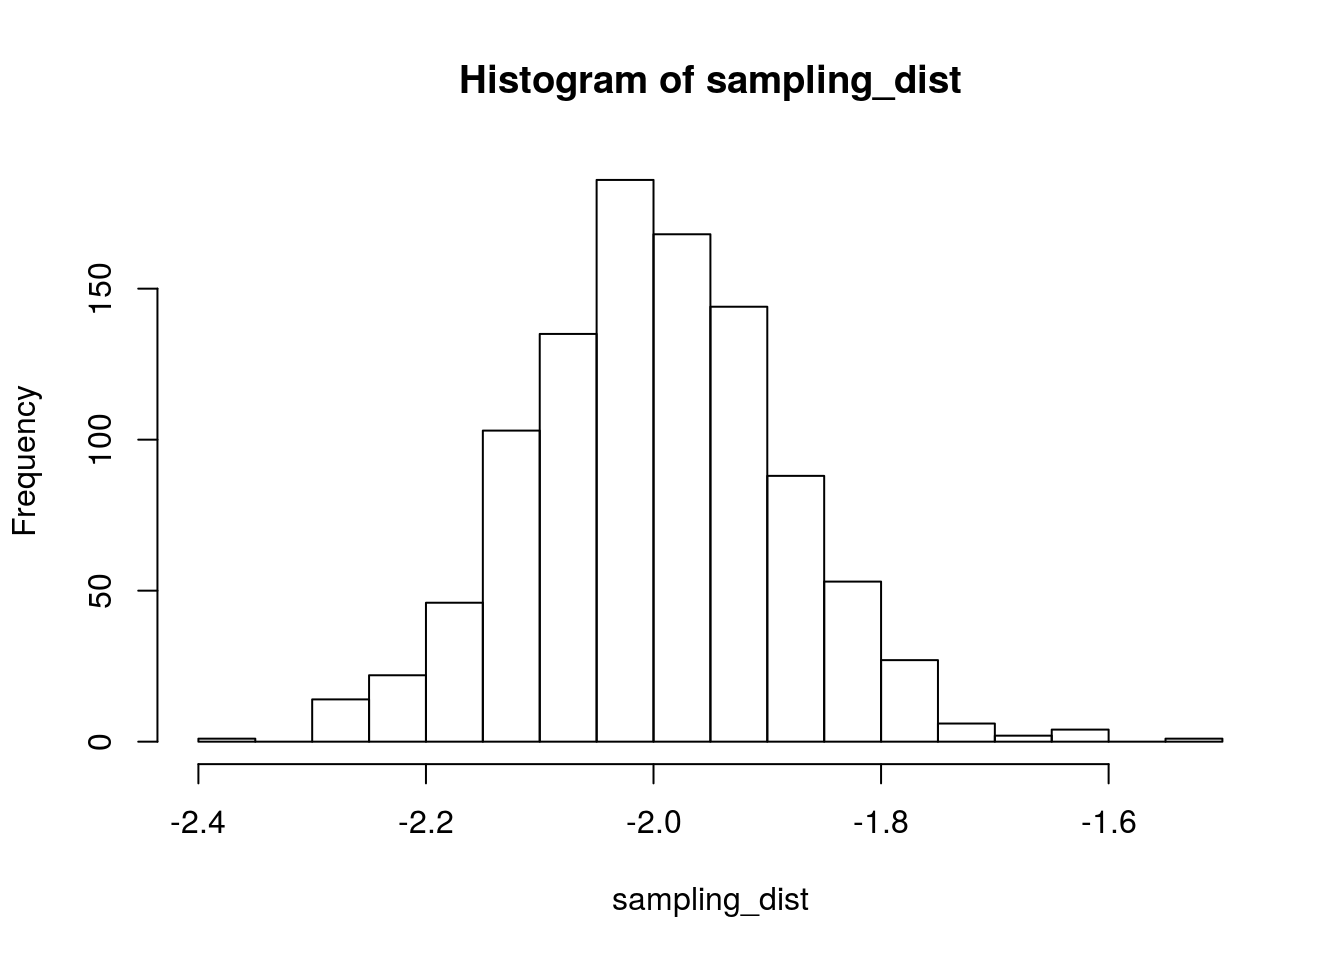
\includegraphics{pdaps_files/figure-latex/mc-ols-clt-1.pdf}

For loops are fun, but don't overuse them. Many simple operations are \textbf{vectorized} and don't require a loop. For example, suppose you want to take the square of a sequence of numbers. You could use a for loop \ldots{}

\begin{Shaded}
\begin{Highlighting}[]
\NormalTok{input \textless{}{-}}\StringTok{ }\KeywordTok{c}\NormalTok{(}\DecValTok{1}\NormalTok{, }\DecValTok{3}\NormalTok{, }\DecValTok{7}\NormalTok{, }\DecValTok{29}\NormalTok{)}
\NormalTok{output \textless{}{-}}\StringTok{ }\KeywordTok{rep}\NormalTok{(}\OtherTok{NA}\NormalTok{, }\KeywordTok{length}\NormalTok{(input))}

\ControlFlowTok{for}\NormalTok{ (i }\ControlFlowTok{in} \DecValTok{1}\OperatorTok{:}\KeywordTok{length}\NormalTok{(input)) \{}
\NormalTok{  output[i] \textless{}{-}}\StringTok{ }\NormalTok{input[i]}\OperatorTok{\^{}}\DecValTok{2}
\NormalTok{\}}

\NormalTok{output}
\end{Highlighting}
\end{Shaded}

\begin{verbatim}
## [1]   1   9  49 841
\end{verbatim}

\ldots{} but it's faster (in terms of computational speed) and easier to just take advantage of vectorization:

\begin{Shaded}
\begin{Highlighting}[]
\NormalTok{input}\OperatorTok{\^{}}\DecValTok{2}
\end{Highlighting}
\end{Shaded}

\begin{verbatim}
## [1]   1   9  49 841
\end{verbatim}

Another useful piece of control flow is \textbf{if/else statements}. These check a logical condition---an expression whose value is \texttt{TRUE} or \texttt{FALSE}---and run different code depending on the value of the expression. (You may want to catch up on the comparison operators: \texttt{==}, \texttt{\textgreater{}}, \texttt{\textgreater{}=}, \texttt{\textless{}}, \texttt{\textless{}=}, etc.)

Let's edit the \texttt{ols\_coef} function to allow us to extract the intercept instead of the slope. We'll add another argument to the function, and implement the option using an if/else statement.

\begin{Shaded}
\begin{Highlighting}[]
\NormalTok{ols\_coef \textless{}{-}}\StringTok{ }\ControlFlowTok{function}\NormalTok{(x, y, }\DataTypeTok{slope =} \OtherTok{TRUE}\NormalTok{) \{}
\NormalTok{  fit \textless{}{-}}\StringTok{ }\KeywordTok{lm}\NormalTok{(y }\OperatorTok{\textasciitilde{}}\StringTok{ }\NormalTok{x)}

  \ControlFlowTok{if}\NormalTok{ (slope) \{}
\NormalTok{    cf \textless{}{-}}\StringTok{ }\KeywordTok{coef}\NormalTok{(fit)[}\DecValTok{2}\NormalTok{]}
\NormalTok{  \} }\ControlFlowTok{else}\NormalTok{ \{}
\NormalTok{    cf \textless{}{-}}\StringTok{ }\KeywordTok{coef}\NormalTok{(fit)[}\DecValTok{1}\NormalTok{]}
\NormalTok{  \}}

  \KeywordTok{return}\NormalTok{(cf)}
\NormalTok{\}}
\end{Highlighting}
\end{Shaded}

Here's how the \texttt{if}/\texttt{else} block in the middle of the function works.
The first line checks the \texttt{slope} variable.
If it's \texttt{TRUE}, then it runs the first set of brackets (extract the slope).
If not, then it skips that, and runs the second set of brackets (extract the intercept).

Also notice how we wrote \texttt{slope\ =\ TRUE} into the arguments of the function.
This sets \texttt{TRUE} as the default value, so if we call \texttt{ols\_coef()} without explicitly specifying the \texttt{slope} argument, it will assume we wanted it to be \texttt{TRUE}.

\begin{Shaded}
\begin{Highlighting}[]
\KeywordTok{ols\_coef}\NormalTok{(x, y)}
\end{Highlighting}
\end{Shaded}

\begin{verbatim}
##         x 
## -2.126934
\end{verbatim}

\begin{Shaded}
\begin{Highlighting}[]
\KeywordTok{ols\_coef}\NormalTok{(x, y, }\DataTypeTok{slope =} \OtherTok{TRUE}\NormalTok{)}
\end{Highlighting}
\end{Shaded}

\begin{verbatim}
##         x 
## -2.126934
\end{verbatim}

\begin{Shaded}
\begin{Highlighting}[]
\KeywordTok{ols\_coef}\NormalTok{(x, y, }\DataTypeTok{slope =} \OtherTok{FALSE}\NormalTok{)}
\end{Highlighting}
\end{Shaded}

\begin{verbatim}
## (Intercept) 
##     1.11694
\end{verbatim}

There is a vectorized version of if/else statements called, naturally, the \texttt{ifelse} function. This function takes three arguments, each a vector of the same length: (1) a logical condition, (2) an output value if the condition is \texttt{TRUE}, (3) an output value if the condition is \texttt{FALSE}.

\begin{Shaded}
\begin{Highlighting}[]
\NormalTok{x \textless{}{-}}\StringTok{ }\DecValTok{1}\OperatorTok{:}\DecValTok{10}
\NormalTok{big\_x \textless{}{-}}\StringTok{ }\NormalTok{x }\OperatorTok{*}\StringTok{ }\DecValTok{100}
\NormalTok{small\_x \textless{}{-}}\StringTok{ }\NormalTok{x }\OperatorTok{*}\StringTok{ }\DecValTok{{-}100}

\KeywordTok{ifelse}\NormalTok{(x }\OperatorTok{\textgreater{}}\StringTok{ }\DecValTok{5}\NormalTok{, big\_x, small\_x)}
\end{Highlighting}
\end{Shaded}

\begin{verbatim}
##  [1] -100 -200 -300 -400 -500  600  700  800  900 1000
\end{verbatim}

Functions, for loops, and if/else statements are just a few of the useful tools for programming in R.\footnote{Others include the \texttt{replicate} function, the \texttt{apply} family of functions (\texttt{sapply}, \texttt{lapply}, \texttt{tapply}, \texttt{mapply}, \ldots), the \textbf{foreach} package, the \textbf{purrr} package, just to name a few of the most useful off the top of my head.} But even these simple tools are enough to allow you to do much more at scale than you could with a copy-paste philosophy.

\hypertarget{data}{%
\chapter{Working with Data}\label{data}}

\emph{Some material in this chapter is adapted from notes \href{http://mdilorenzo.github.io}{Matt DiLorenzo} wrote for the Spring 2016 session of PSCI 8357.}

In your careers as social scientists, starting with your dissertation research---if not earlier---you will probably spend more time collecting, merging, and cleaning data than you will on statistical analysis. So it's worth taking some time to learn how to do this well.

Best practices for data management can be summarized in a single sentence: \emph{Record and document everything you do to the data.}

The first corollary of this principle is that raw data is sacrosanct. You should never edit raw data ``in place''. Once you download the raw data file, that file should never change.\footnote{Even if it's data you collected yourself, that data should still have a ``canonical'' representation that never gets overwritten. See \citet{Leek:2015uw} for more on distributing your own data.}

In almost any non-trivial analysis, the ``final'' data---the format you plug into your analysis---will differ significantly from the raw data. It may consist of information merged from multiple sources. The variables may have been transformed, aggregated, or otherwise altered. The unit of observation may even differ from the original source. You must document every one of these changes, so that another researcher working from the exact same raw data will end up with the exact same final data.

The most sensible way to achieve this level of reproducibility is to do all of your data merging and cleaning in a script. In other words, no going into Excel and mucking around manually. Like any other piece of your analysis, your pipeline from raw data to final data should follow the \protect\hyperlink{programming}{principles of programming} that we discussed last week.

Luckily for you,\footnote{But not for me, because these tools didn't exist when I was a PhD student. Yes, I am old.} the \textbf{tidyverse} suite of R packages (including \textbf{dplyr}, \textbf{tidyr}, and others) makes it easy to script your ``data pipeline''.

\begin{Shaded}
\begin{Highlighting}[]
\KeywordTok{library}\NormalTok{(}\StringTok{"tidyverse"}\NormalTok{)}
\end{Highlighting}
\end{Shaded}

\hypertarget{loading}{%
\section{Loading}\label{loading}}

The first step in working with data is to acquire some data. Depending on the nature of your research, you will be getting some or all of your data from sources available online. When you download data from online repositories, you should keep track of where you got it from. The best way to do so is---you guessed it---to script your data acquisition.

The R function \texttt{download.file()} is the easiest way to download files from URLs from within R. Just specify where you're getting the file from and where you want it to go. For the examples today, we'll use an ``untidied'' version of the World Development Indicators data from the World Bank that I've posted to my website.

\begin{Shaded}
\begin{Highlighting}[]
\KeywordTok{download.file}\NormalTok{(}\DataTypeTok{url =} \StringTok{"http://bkenkel.com/files/untidy{-}data.csv"}\NormalTok{,}
              \DataTypeTok{destfile =} \StringTok{"my{-}untidy{-}data.csv"}\NormalTok{)}
\end{Highlighting}
\end{Shaded}

Once you've got the file stored locally, use the utilities from the \textbf{readr} package (part of \textbf{tidyverse}) to read it into R as a data frame.\footnote{More precisely, the \textbf{readr} functions produce output of class \texttt{"tbl\_df"} (pronounced ``tibble diff,'' I'm told), which are like data frames but better. See \texttt{help(package\ =\ "tibble")} for what can be done with \texttt{tbl\_df}s.} We have a CSV file, so we will use \texttt{read\_csv}. See \texttt{help(package\ =\ "readr")} for other possibilities.
\texttt{read\_csv} (with an underscore) is typically better than R's built-in \texttt{read.csv} (with a dot), as it reads files faster and processes them more cleanly.

\begin{Shaded}
\begin{Highlighting}[]
\NormalTok{untidy\_data \textless{}{-}}\StringTok{ }\KeywordTok{read\_csv}\NormalTok{(}\DataTypeTok{file =} \StringTok{"my{-}untidy{-}data.csv"}\NormalTok{)}
\end{Highlighting}
\end{Shaded}

\begin{verbatim}
## 
## -- Column specification ---------------------------------------------------------------------------------
## cols(
##   country = col_character(),
##   gdp.2005 = col_double(),
##   gdp.2006 = col_double(),
##   gdp.2007 = col_double(),
##   gdp.2008 = col_double(),
##   pop.2005 = col_double(),
##   pop.2006 = col_double(),
##   pop.2007 = col_double(),
##   pop.2008 = col_double(),
##   unemp.2005 = col_double(),
##   unemp.2006 = col_double(),
##   unemp.2007 = col_double(),
##   unemp.2008 = col_double()
## )
\end{verbatim}

Remember that each column of a data frame might be a different type, or more formally \emph{class}, of object. \texttt{read\_csv} and its ilk try to guess the type of data each column contains: character, integer, decimal number (``double'' in programming-speak), or something else. The readout above tells you what guesses it made. If it gets something wrong---say, reading a column as numbers that ought to be characters---you can use the \texttt{col\_types} argument to set it straight.

FYI, you could also run \texttt{read\_csv()} directly on a URL, as in:

\begin{Shaded}
\begin{Highlighting}[]
\KeywordTok{read\_csv}\NormalTok{(}\StringTok{"http://bkenkel.com/files/untidy{-}data.csv"}\NormalTok{)}
\end{Highlighting}
\end{Shaded}

However, in analyses intended for publication, it's usually preferable to download and save the raw data. What's stored at a URL might change or disappear, and you'll need to have a hard copy of the raw data for replication purposes.

Now let's take a look at the data we've just loaded in.

\begin{Shaded}
\begin{Highlighting}[]
\NormalTok{untidy\_data}
\end{Highlighting}
\end{Shaded}

\begin{verbatim}
## # A tibble: 215 x 13
##   country gdp.2005 gdp.2006 gdp.2007 gdp.2008 pop.2005 pop.2006 pop.2007
##   <chr>      <dbl>    <dbl>    <dbl>    <dbl>    <dbl>    <dbl>    <dbl>
## 1 AD          3.85     4.03     4.03     3.68   0.0789   0.0810   0.0827
## 2 AE        257.     283.     292.     301.     4.59     5.30     6.17  
## 3 AF          9.16     9.66    11.0     11.4   25.7     26.4     27.1   
## 4 AG          1.15     1.29     1.41     1.41   0.0815   0.0827   0.0840
## 5 AL          9.22     9.77    10.4     11.1    3.01     2.99     2.97  
## # ... with 210 more rows, and 5 more variables: pop.2008 <dbl>,
## #   unemp.2005 <dbl>, unemp.2006 <dbl>, unemp.2007 <dbl>, unemp.2008 <dbl>
\end{verbatim}

We have a \texttt{country} variable giving country abbreviations. The other variables are numerical values: the country's GDP in 2005, 2006, 2007, and 2008; then the same for population and unemployment. Let's get this into a format we could use for analysis.

\hypertarget{tidying}{%
\section{Tidying}\label{tidying}}

\citet{Wickham:2014vp} outlines three qualities that make data ``tidy'':

\begin{enumerate}
\def\labelenumi{\arabic{enumi}.}
\tightlist
\item
  Each variable forms a column.
\item
  Each observation forms a row.
\item
  Each type of observational unit forms a table.
\end{enumerate}

For one thing, this means that whether a dataset is tidy or not depends---at least in part (some data collections are messy from any angle)---on the purpose it's being analyzed for.

Each row of \texttt{untidy\_data} is a country. In observational studies in comparative politics and international relations, more commonly the unit of observation is the country-year.\footnote{Yes, this kind of huge cross-country analysis has fallen out of favor as we've become more attentive to causal inference. But wait until later in the semester to worry about that!} How can we take \texttt{untidy\_data} and easily make it into country-year data?

We'll use the \textbf{tidyr} package (again, part of \textbf{tidyverse}) to clean up this data. The biggest problem right now is that each column, besides the country identifier, really encodes two pieces of information: the year of observation and the variable being observed. To deal with this, we'll have to first transform the data from one untidy format to another. We're going to use the \texttt{pivot\_longer()} function to make each row a country-year-variable.

What \texttt{pivot\_longer()} does is make a row for each entry from a set of columns. It's probably easiest to understand it by seeing it in practice:

\begin{Shaded}
\begin{Highlighting}[]
\NormalTok{long\_data \textless{}{-}}\StringTok{ }\KeywordTok{pivot\_longer}\NormalTok{(untidy\_data,}
                          \DataTypeTok{cols =} \KeywordTok{starts\_with}\NormalTok{(}\KeywordTok{c}\NormalTok{(}\StringTok{"gdp"}\NormalTok{, }\StringTok{"pop"}\NormalTok{, }\StringTok{"unemp"}\NormalTok{)))}
\NormalTok{long\_data}
\end{Highlighting}
\end{Shaded}

\begin{verbatim}
## # A tibble: 2,580 x 3
##   country name      value
##   <chr>   <chr>     <dbl>
## 1 AD      gdp.2005 3.85  
## 2 AD      gdp.2006 4.03  
## 3 AD      gdp.2007 4.03  
## 4 AD      gdp.2008 3.68  
## 5 AD      pop.2005 0.0789
## # ... with 2,575 more rows
\end{verbatim}

The \texttt{cols} argument tells \texttt{pivot\_longer()} which columns to collect.
The code here specifies that it be all of the columns starting with ``gdp'', ``pop'', or ``unemp''.
As it happens, we could have achieved the same result by using \texttt{cols\ =\ ends\_with(c("2005",\ "2006",\ "2007",\ "2008"))}.
To select all columns, we instead would have used \texttt{cols\ =\ everything()}.
For additional ways of selecting columns, see the help page \texttt{?tidyselect::select\_helpers}.

Now we have a new problem, which is that the \texttt{name} column encodes two pieces of information: the variable and the year of its observation. \textbf{tidyr} provides the \texttt{separate()} function to solve that, splitting a single variable into two.

\begin{Shaded}
\begin{Highlighting}[]
\NormalTok{long\_data \textless{}{-}}\StringTok{ }\KeywordTok{separate}\NormalTok{(long\_data,}
                      \DataTypeTok{col =} \StringTok{"name"}\NormalTok{,}
                      \DataTypeTok{into =} \KeywordTok{c}\NormalTok{(}\StringTok{"var"}\NormalTok{, }\StringTok{"year"}\NormalTok{))}
\NormalTok{long\_data}
\end{Highlighting}
\end{Shaded}

\begin{verbatim}
## # A tibble: 2,580 x 4
##   country var   year   value
##   <chr>   <chr> <chr>  <dbl>
## 1 AD      gdp   2005  3.85  
## 2 AD      gdp   2006  4.03  
## 3 AD      gdp   2007  4.03  
## 4 AD      gdp   2008  3.68  
## 5 AD      pop   2005  0.0789
## # ... with 2,575 more rows
\end{verbatim}

So now we have country-year-variable data, with the year and variable conveniently stored in different columns. To turn this into country-year data, we can use the \texttt{pivot\_wider()} function, which is like the inverse of \texttt{pivot\_longer()}. \texttt{pivot\_wider()} takes a key column and a value column, and turns each different key into a column of its own.

\begin{Shaded}
\begin{Highlighting}[]
\NormalTok{clean\_data \textless{}{-}}\StringTok{ }\KeywordTok{pivot\_wider}\NormalTok{(long\_data,}
                          \DataTypeTok{names\_from =} \StringTok{"var"}\NormalTok{,}
                          \DataTypeTok{values\_from =} \StringTok{"value"}\NormalTok{)}
\NormalTok{clean\_data}
\end{Highlighting}
\end{Shaded}

\begin{verbatim}
## # A tibble: 860 x 5
##   country year     gdp    pop unemp
##   <chr>   <chr>  <dbl>  <dbl> <dbl>
## 1 AD      2005    3.85 0.0789 NA   
## 2 AD      2006    4.03 0.0810 NA   
## 3 AD      2007    4.03 0.0827 NA   
## 4 AD      2008    3.68 0.0839 NA   
## 5 AE      2005  257.   4.59    3.12
## # ... with 855 more rows
\end{verbatim}

When using \texttt{pivot\_wider()} on data that you didn't previously \texttt{pivot\_longer()}, be sure to set the \texttt{values\_fill} argument to tell it how to fill in empty cells. A simple example:

\begin{Shaded}
\begin{Highlighting}[]
\NormalTok{test\_data}
\end{Highlighting}
\end{Shaded}

\begin{verbatim}
## # A tibble: 3 x 3
##   id      name  value
##   <chr>   <chr> <dbl>
## 1 brenton a        10
## 2 brenton b        20
## 3 patrick b         5
\end{verbatim}

\begin{Shaded}
\begin{Highlighting}[]
\KeywordTok{pivot\_wider}\NormalTok{(test\_data, }\DataTypeTok{names\_from =} \StringTok{"name"}\NormalTok{, }\DataTypeTok{values\_from =} \StringTok{"value"}\NormalTok{)}
\end{Highlighting}
\end{Shaded}

\begin{verbatim}
## # A tibble: 2 x 3
##   id          a     b
##   <chr>   <dbl> <dbl>
## 1 brenton    10    20
## 2 patrick    NA     5
\end{verbatim}

\begin{Shaded}
\begin{Highlighting}[]
\KeywordTok{pivot\_wider}\NormalTok{(test\_data, }\DataTypeTok{names\_from =} \StringTok{"name"}\NormalTok{, }\DataTypeTok{values\_from =} \StringTok{"value"}\NormalTok{, }\DataTypeTok{values\_fill =} \DecValTok{0}\NormalTok{)}
\end{Highlighting}
\end{Shaded}

\begin{verbatim}
## # A tibble: 2 x 3
##   id          a     b
##   <chr>   <dbl> <dbl>
## 1 brenton    10    20
## 2 patrick     0     5
\end{verbatim}

One more important note on \textbf{tidyverse} semantics. It includes a fabulous feature called the \emph{pipe}, \texttt{\%\textgreater{}\%}, which makes it easy to string together a truly mind-boggling number of commands.

In pipe syntax, \texttt{x\ \%\textgreater{}\%\ f()} is equivalent to \texttt{f(x)}. That seems like a wasteful and confusing way to write \texttt{f(x)}, and it is. But if you want to string together a bunch of commands, it's much easier to comprehend

\begin{Shaded}
\begin{Highlighting}[]
\NormalTok{x }\OperatorTok{\%\textgreater{}\%}
\StringTok{  }\KeywordTok{f}\NormalTok{() }\OperatorTok{\%\textgreater{}\%}
\StringTok{  }\KeywordTok{g}\NormalTok{() }\OperatorTok{\%\textgreater{}\%}
\StringTok{  }\KeywordTok{h}\NormalTok{() }\OperatorTok{\%\textgreater{}\%}
\StringTok{  }\KeywordTok{i}\NormalTok{()}
\end{Highlighting}
\end{Shaded}

than \texttt{i(h(g(f(x))))}.

You can pass function arguments using the pipe too. For example, \texttt{f(x,\ bear\ =\ "moose")} is equivalent to \texttt{x\ \%\textgreater{}\%\ f(bear\ =\ "moose")}.

The key thing about the \textbf{tidyverse} functions is that each of them takes a data frame as its first argument, and returns a data frame as its output. This makes them highly amenable to piping. For example, we can combine all three steps of our tidying above with a single command, thanks to the pipe:

\begin{Shaded}
\begin{Highlighting}[]
\NormalTok{untidy\_data }\OperatorTok{\%\textgreater{}\%}
\StringTok{  }\KeywordTok{pivot\_longer}\NormalTok{(}\DataTypeTok{cols =} \KeywordTok{starts\_with}\NormalTok{(}\KeywordTok{c}\NormalTok{(}\StringTok{"gdp"}\NormalTok{, }\StringTok{"pop"}\NormalTok{, }\StringTok{"unemp"}\NormalTok{))) }\OperatorTok{\%\textgreater{}\%}
\StringTok{  }\KeywordTok{separate}\NormalTok{(}\DataTypeTok{col =} \StringTok{"name"}\NormalTok{,}
           \DataTypeTok{into =} \KeywordTok{c}\NormalTok{(}\StringTok{"var"}\NormalTok{, }\StringTok{"year"}\NormalTok{)) }\OperatorTok{\%\textgreater{}\%}
\StringTok{  }\KeywordTok{pivot\_wider}\NormalTok{(}\DataTypeTok{names\_from =} \StringTok{"var"}\NormalTok{,}
              \DataTypeTok{values\_from =} \StringTok{"value"}\NormalTok{)}
\end{Highlighting}
\end{Shaded}

\begin{verbatim}
## # A tibble: 860 x 5
##   country year     gdp    pop unemp
##   <chr>   <chr>  <dbl>  <dbl> <dbl>
## 1 AD      2005    3.85 0.0789 NA   
## 2 AD      2006    4.03 0.0810 NA   
## 3 AD      2007    4.03 0.0827 NA   
## 4 AD      2008    3.68 0.0839 NA   
## 5 AE      2005  257.   4.59    3.12
## # ... with 855 more rows
\end{verbatim}

Without the pipe, if we wanted to run all those commands together, we would have to write:

\begin{Shaded}
\begin{Highlighting}[]
\KeywordTok{pivot\_wider}\NormalTok{(}\KeywordTok{separate}\NormalTok{(}\KeywordTok{pivot\_longer}\NormalTok{(untidy\_data,}
                                  \DataTypeTok{cols =} \KeywordTok{starts\_with}\NormalTok{(}\KeywordTok{c}\NormalTok{(}\StringTok{"gdp"}\NormalTok{, }\StringTok{"pop"}\NormalTok{, }\StringTok{"unemp"}\NormalTok{))),}
                     \DataTypeTok{col =} \StringTok{"name"}\NormalTok{,}
                     \DataTypeTok{into =} \KeywordTok{c}\NormalTok{(}\StringTok{"var"}\NormalTok{, }\StringTok{"year"}\NormalTok{)),}
            \DataTypeTok{names\_from =} \StringTok{"var"}\NormalTok{,}
            \DataTypeTok{values\_from =} \StringTok{"value"}\NormalTok{)}
\end{Highlighting}
\end{Shaded}

Going back to last week's dictum of ``write programs for people'': even though this would have the same computational result, it's much harder for a human (your future self or a coauthor) to parse what the code is trying to do.

\hypertarget{transforming-and-aggregating}{%
\section{Transforming and Aggregating}\label{transforming-and-aggregating}}

Tidying the data usually isn't the end of the process. If you want to perform further calculations on the raw, that's where the tools in \textbf{dplyr} (part of, you guessed it, the \textbf{tidyverse}) come in.

Perhaps the simplest \textbf{dplyr} function (or ``verb'', as the R hipsters would say) is \texttt{rename()}, which lets you rename columns.

\begin{Shaded}
\begin{Highlighting}[]
\NormalTok{clean\_data }\OperatorTok{\%\textgreater{}\%}
\StringTok{  }\KeywordTok{rename}\NormalTok{(}\DataTypeTok{gross\_domestic\_product =}\NormalTok{ gdp)}
\end{Highlighting}
\end{Shaded}

\begin{verbatim}
## # A tibble: 860 x 5
##   country year  gross_domestic_product    pop unemp
##   <chr>   <chr>                  <dbl>  <dbl> <dbl>
## 1 AD      2005                    3.85 0.0789 NA   
## 2 AD      2006                    4.03 0.0810 NA   
## 3 AD      2007                    4.03 0.0827 NA   
## 4 AD      2008                    3.68 0.0839 NA   
## 5 AE      2005                  257.   4.59    3.12
## # ... with 855 more rows
\end{verbatim}

The \textbf{dplyr} functions, like the vast majority of R functions, do not modify their inputs. In other words, running \texttt{rename()} on \texttt{clean\_data} will return a renamed copy of \texttt{clean\_data}, but won't overwrite the original.

\begin{Shaded}
\begin{Highlighting}[]
\NormalTok{clean\_data}
\end{Highlighting}
\end{Shaded}

\begin{verbatim}
## # A tibble: 860 x 5
##   country year     gdp    pop unemp
##   <chr>   <chr>  <dbl>  <dbl> <dbl>
## 1 AD      2005    3.85 0.0789 NA   
## 2 AD      2006    4.03 0.0810 NA   
## 3 AD      2007    4.03 0.0827 NA   
## 4 AD      2008    3.68 0.0839 NA   
## 5 AE      2005  257.   4.59    3.12
## # ... with 855 more rows
\end{verbatim}

If you wanted to make the change stick, you would have to run:

\begin{Shaded}
\begin{Highlighting}[]
\NormalTok{clean\_data \textless{}{-}}\StringTok{ }\NormalTok{clean\_data }\OperatorTok{\%\textgreater{}\%}
\StringTok{  }\KeywordTok{rename}\NormalTok{(}\DataTypeTok{gross\_domestic\_product =}\NormalTok{ gdp)}
\end{Highlighting}
\end{Shaded}

\texttt{select()} lets you keep a couple of columns and drop all the others. Or vice versa if you use minus signs.

\begin{Shaded}
\begin{Highlighting}[]
\NormalTok{clean\_data }\OperatorTok{\%\textgreater{}\%}
\StringTok{  }\KeywordTok{select}\NormalTok{(country, gdp)}
\end{Highlighting}
\end{Shaded}

\begin{verbatim}
## # A tibble: 860 x 2
##   country    gdp
##   <chr>    <dbl>
## 1 AD        3.85
## 2 AD        4.03
## 3 AD        4.03
## 4 AD        3.68
## 5 AE      257.  
## # ... with 855 more rows
\end{verbatim}

\begin{Shaded}
\begin{Highlighting}[]
\NormalTok{clean\_data }\OperatorTok{\%\textgreater{}\%}
\StringTok{  }\KeywordTok{select}\NormalTok{(}\OperatorTok{{-}}\NormalTok{pop)}
\end{Highlighting}
\end{Shaded}

\begin{verbatim}
## # A tibble: 860 x 4
##   country year     gdp unemp
##   <chr>   <chr>  <dbl> <dbl>
## 1 AD      2005    3.85 NA   
## 2 AD      2006    4.03 NA   
## 3 AD      2007    4.03 NA   
## 4 AD      2008    3.68 NA   
## 5 AE      2005  257.    3.12
## # ... with 855 more rows
\end{verbatim}

As we saw above, you can also select columns based on how their names start or end, or with even more complex criteria.
See \texttt{?tidyselect::select\_helpers}.

\begin{Shaded}
\begin{Highlighting}[]
\NormalTok{untidy\_data }\OperatorTok{\%\textgreater{}\%}
\StringTok{  }\KeywordTok{select}\NormalTok{(country, }\KeywordTok{starts\_with}\NormalTok{(}\StringTok{"gdp"}\NormalTok{))}
\end{Highlighting}
\end{Shaded}

\begin{verbatim}
## # A tibble: 215 x 5
##   country gdp.2005 gdp.2006 gdp.2007 gdp.2008
##   <chr>      <dbl>    <dbl>    <dbl>    <dbl>
## 1 AD          3.85     4.03     4.03     3.68
## 2 AE        257.     283.     292.     301.  
## 3 AF          9.16     9.66    11.0     11.4 
## 4 AG          1.15     1.29     1.41     1.41
## 5 AL          9.22     9.77    10.4     11.1 
## # ... with 210 more rows
\end{verbatim}

\begin{Shaded}
\begin{Highlighting}[]
\NormalTok{untidy\_data }\OperatorTok{\%\textgreater{}\%}
\StringTok{  }\KeywordTok{select}\NormalTok{(country, }\KeywordTok{ends\_with}\NormalTok{(}\StringTok{"2005"}\NormalTok{))}
\end{Highlighting}
\end{Shaded}

\begin{verbatim}
## # A tibble: 215 x 4
##   country gdp.2005 pop.2005 unemp.2005
##   <chr>      <dbl>    <dbl>      <dbl>
## 1 AD          3.85   0.0789      NA   
## 2 AE        257.     4.59         3.12
## 3 AF          9.16  25.7          2.94
## 4 AG          1.15   0.0815      NA   
## 5 AL          9.22   3.01        16.9 
## # ... with 210 more rows
\end{verbatim}

\texttt{mutate()} lets you create new variables that are transformations of old ones.

\begin{Shaded}
\begin{Highlighting}[]
\NormalTok{clean\_data }\OperatorTok{\%\textgreater{}\%}
\StringTok{  }\KeywordTok{mutate}\NormalTok{(}\DataTypeTok{gdppc =}\NormalTok{ gdp }\OperatorTok{/}\StringTok{ }\NormalTok{pop,}
         \DataTypeTok{log\_gdppc =} \KeywordTok{log}\NormalTok{(gdppc))}
\end{Highlighting}
\end{Shaded}

\begin{verbatim}
## # A tibble: 860 x 7
##   country year     gdp    pop unemp gdppc log_gdppc
##   <chr>   <chr>  <dbl>  <dbl> <dbl> <dbl>     <dbl>
## 1 AD      2005    3.85 0.0789 NA     48.8      3.89
## 2 AD      2006    4.03 0.0810 NA     49.7      3.91
## 3 AD      2007    4.03 0.0827 NA     48.7      3.89
## 4 AD      2008    3.68 0.0839 NA     43.9      3.78
## 5 AE      2005  257.   4.59    3.12  56.1      4.03
## # ... with 855 more rows
\end{verbatim}

\texttt{filter()} cuts down the data according to the logical condition(s) you specify.

\begin{Shaded}
\begin{Highlighting}[]
\NormalTok{clean\_data }\OperatorTok{\%\textgreater{}\%}
\StringTok{  }\KeywordTok{filter}\NormalTok{(year }\OperatorTok{==}\StringTok{ }\DecValTok{2006}\NormalTok{)}
\end{Highlighting}
\end{Shaded}

\begin{verbatim}
## # A tibble: 215 x 5
##   country year     gdp     pop unemp
##   <chr>   <chr>  <dbl>   <dbl> <dbl>
## 1 AD      2006    4.03  0.0810 NA   
## 2 AE      2006  283.    5.30    2.77
## 3 AF      2006    9.66 26.4     2.83
## 4 AG      2006    1.29  0.0827 NA   
## 5 AL      2006    9.77  2.99   16.4 
## # ... with 210 more rows
\end{verbatim}

\texttt{summarise()} calculates summaries of the data. For example, let's find the maximum unemployment rate.

\begin{Shaded}
\begin{Highlighting}[]
\NormalTok{clean\_data }\OperatorTok{\%\textgreater{}\%}
\StringTok{  }\KeywordTok{summarise}\NormalTok{(}\DataTypeTok{max\_unemp =} \KeywordTok{max}\NormalTok{(unemp, }\DataTypeTok{na.rm =} \OtherTok{TRUE}\NormalTok{))}
\end{Highlighting}
\end{Shaded}

\begin{verbatim}
## # A tibble: 1 x 1
##   max_unemp
##       <dbl>
## 1      37.2
\end{verbatim}

This seems sort of useless, until you combine it with the \texttt{group\_by()} function. If you group the data before \texttt{summarise}-ing it, you'll calculate a separate summary for each group. For example, let's calculate the maximum unemployment rate for each year in the data.

\begin{Shaded}
\begin{Highlighting}[]
\NormalTok{clean\_data }\OperatorTok{\%\textgreater{}\%}
\StringTok{  }\KeywordTok{group\_by}\NormalTok{(year) }\OperatorTok{\%\textgreater{}\%}
\StringTok{  }\KeywordTok{summarise}\NormalTok{(}\DataTypeTok{max\_unemp =} \KeywordTok{max}\NormalTok{(unemp, }\DataTypeTok{na.rm =} \OtherTok{TRUE}\NormalTok{))}
\end{Highlighting}
\end{Shaded}

\begin{verbatim}
## # A tibble: 4 x 2
##   year  max_unemp
## * <chr>     <dbl>
## 1 2005       37.2
## 2 2006       36.0
## 3 2007       34.9
## 4 2008       33.8
\end{verbatim}

\texttt{summarise()} produces a ``smaller'' data frame than the input---one row per group. If you want to do something similar, but preserving the structure of the original data, use \texttt{mutate} in combination with \texttt{group\_by}.

\begin{Shaded}
\begin{Highlighting}[]
\NormalTok{clean\_data }\OperatorTok{\%\textgreater{}\%}
\StringTok{  }\KeywordTok{filter}\NormalTok{(}\OperatorTok{!}\KeywordTok{is.na}\NormalTok{(unemp)) }\OperatorTok{\%\textgreater{}\%}
\StringTok{  }\KeywordTok{group\_by}\NormalTok{(year) }\OperatorTok{\%\textgreater{}\%}
\StringTok{  }\KeywordTok{mutate}\NormalTok{(}\DataTypeTok{max\_unemp =} \KeywordTok{max}\NormalTok{(unemp),}
         \DataTypeTok{unemp\_over\_max =}\NormalTok{ unemp }\OperatorTok{/}\StringTok{ }\NormalTok{max\_unemp) }\OperatorTok{\%\textgreater{}\%}
\StringTok{  }\KeywordTok{select}\NormalTok{(country, year, }\KeywordTok{contains}\NormalTok{(}\StringTok{"unemp"}\NormalTok{))}
\end{Highlighting}
\end{Shaded}

\begin{verbatim}
## # A tibble: 744 x 5
## # Groups:   year [4]
##   country year  unemp max_unemp unemp_over_max
##   <chr>   <chr> <dbl>     <dbl>          <dbl>
## 1 AE      2005   3.12      37.2         0.0838
## 2 AE      2006   2.77      36.0         0.0770
## 3 AE      2007   2.47      34.9         0.0706
## 4 AE      2008   2.33      33.8         0.0691
## 5 AF      2005   2.94      37.2         0.0790
## # ... with 739 more rows
\end{verbatim}

This gives us back the original data, but with a \texttt{max\_unemp} variable recording the highest unemployment level that year. We can then calculate each individual country's unemployment as a percentage of the maximum. Whether grouped \texttt{mutate} or \texttt{summarise} is better depends, of course, on the purpose and structure of your analysis.

\hypertarget{merging}{%
\section{Merging}\label{merging}}

Particularly if you do observational work, you'll often be merging together data from multiple sources.
The key to merging data from separate tables is to have consistent identifiers across tables. For example, if you run an experiment, you might have demographic data on each subject in one table, and each subject's response to treatment in another table. Naturally, you'll want to have a subject identifier that ``links'' the records across tables, as in the following hypothetical example.

\begin{Shaded}
\begin{Highlighting}[]
\NormalTok{subject\_data}
\end{Highlighting}
\end{Shaded}

\begin{verbatim}
## # A tibble: 3 x 4
##      id gender loves_bernie does_yoga
##   <dbl> <chr>  <chr>        <chr>    
## 1  1001 male   yes          no       
## 2  1002 female no           yes      
## 3  1003 male   no           no
\end{verbatim}

\begin{Shaded}
\begin{Highlighting}[]
\NormalTok{subject\_response\_data}
\end{Highlighting}
\end{Shaded}

\begin{verbatim}
## # A tibble: 6 x 3
##      id treatment response
##   <dbl> <chr>     <chr>   
## 1  1001 read_book sad     
## 2  1001 watch_tv  sad     
## 3  1002 read_book happy   
## 4  1002 watch_tv  sad     
## 5  1003 read_book sad     
## 6  1003 watch_tv  happy
\end{verbatim}

Let's practice merging data with our cleaned-up country-year data. We'll take two datasets from my website: a country-level dataset with latitudes and longitudes, and a country-year--level dataset with inflation over time.

\begin{Shaded}
\begin{Highlighting}[]
\NormalTok{latlong\_data \textless{}{-}}\StringTok{ }\KeywordTok{read\_csv}\NormalTok{(}\StringTok{"http://bkenkel.com/files/latlong.csv"}\NormalTok{)}
\NormalTok{latlong\_data}
\end{Highlighting}
\end{Shaded}

\begin{verbatim}
## # A tibble: 245 x 3
##   country latitude longitude
##   <chr>      <dbl>     <dbl>
## 1 AD          42.5      1.60
## 2 AE          23.4     53.8 
## 3 AF          33.9     67.7 
## 4 AG          17.1    -61.8 
## 5 AI          18.2    -63.1 
## # ... with 240 more rows
\end{verbatim}

\begin{Shaded}
\begin{Highlighting}[]
\NormalTok{inflation\_data \textless{}{-}}\StringTok{ }\KeywordTok{read\_csv}\NormalTok{(}\StringTok{"http://bkenkel.com/files/inflation.csv"}\NormalTok{)}
\NormalTok{inflation\_data}
\end{Highlighting}
\end{Shaded}

\begin{verbatim}
## # A tibble: 1,070 x 3
##   country  year inflation
##   <chr>   <dbl>     <dbl>
## 1 AD       2004        NA
## 2 AD       2005        NA
## 3 AD       2006        NA
## 4 AD       2007        NA
## 5 AD       2008        NA
## # ... with 1,065 more rows
\end{verbatim}

For your convenience, both of these datasets use the same two-letter country naming scheme as the original data. Unfortunately, out in the real world, data from different sources often use incommensurate naming schemes. Converting from one naming scheme to another is part of the data cleaning process, and it requires careful attention.

\textbf{dplyr} contains various \texttt{\_join()} functions for merging. Each of these take as arguments the two data frames to merge, plus the names of the identifier variables to merge them on. The one I use most often is \texttt{left\_join()}, which keeps every row from the first (``left'') data frame and merges in the columns from the second (``right'') data frame.

For example, let's merge the latitude and longitude data for each country into \texttt{clean\_data}.

\begin{Shaded}
\begin{Highlighting}[]
\KeywordTok{left\_join}\NormalTok{(clean\_data,}
\NormalTok{          latlong\_data,}
          \DataTypeTok{by =} \StringTok{"country"}\NormalTok{)}
\end{Highlighting}
\end{Shaded}

\begin{verbatim}
## # A tibble: 860 x 7
##   country year     gdp    pop unemp latitude longitude
##   <chr>   <chr>  <dbl>  <dbl> <dbl>    <dbl>     <dbl>
## 1 AD      2005    3.85 0.0789 NA        42.5      1.60
## 2 AD      2006    4.03 0.0810 NA        42.5      1.60
## 3 AD      2007    4.03 0.0827 NA        42.5      1.60
## 4 AD      2008    3.68 0.0839 NA        42.5      1.60
## 5 AE      2005  257.   4.59    3.12     23.4     53.8 
## # ... with 855 more rows
\end{verbatim}

Since \texttt{latlong\_data} is country-level, the value is the same for each year. So the merged data contains redundant information. This is one reason to store data observed at different levels in different tables---with redundant observations, it is easier to make errors yet harder to catch them and fix them.

We can also merge data when the identifier is stored across multiple columns, as in the case of our country-year data. But first, a technical note.\footnote{This won't be the case if you got \texttt{clean\_data} by loading it in directly from \texttt{clean-data.csv} on my website, since \texttt{read\_csv()} will have correctly encoded \texttt{year} as an integer.} You might notice that the \texttt{year} column of \texttt{clean\_data} is labeled \texttt{\textless{}chr\textgreater{}}, as in character data. Yet the \texttt{year} column of \texttt{inflation\_data} is labeled \texttt{\textless{}int\textgreater{}}, as in integer data. We can check that by running \texttt{class()} on each respective column.

\begin{Shaded}
\begin{Highlighting}[]
\KeywordTok{class}\NormalTok{(clean\_data}\OperatorTok{$}\NormalTok{year)}
\end{Highlighting}
\end{Shaded}

\begin{verbatim}
## [1] "character"
\end{verbatim}

\begin{Shaded}
\begin{Highlighting}[]
\KeywordTok{class}\NormalTok{(inflation\_data}\OperatorTok{$}\NormalTok{year)}
\end{Highlighting}
\end{Shaded}

\begin{verbatim}
## [1] "numeric"
\end{verbatim}

From R's perspective, the character string \texttt{"1999"} is a very different thing than the integer number \texttt{1999}. Therefore, if we try to merge \texttt{clean\_data} and \texttt{inflation\_data} on the \texttt{year} variable, it will throw an error.

\begin{Shaded}
\begin{Highlighting}[]
\KeywordTok{left\_join}\NormalTok{(clean\_data,}
\NormalTok{          inflation\_data,}
          \DataTypeTok{by =} \KeywordTok{c}\NormalTok{(}\StringTok{"country"}\NormalTok{, }\StringTok{"year"}\NormalTok{))}
\end{Highlighting}
\end{Shaded}

\begin{verbatim}
## Error: Can't join on `x$year` x `y$year` because of incompatible types.
## i `x$year` is of type <character>>.
## i `y$year` is of type <double>>.
\end{verbatim}

To fix this, let's use \texttt{mutate()} to convert the \texttt{year} column of \texttt{clean\_data} to an integer. We probably should have done this in the first place---after all, having the year encoded as a character string would have thrown off plotting functions, statistical functions, or anything else where it would be more natural to treat the year like a number.

\begin{Shaded}
\begin{Highlighting}[]
\NormalTok{clean\_data \textless{}{-}}\StringTok{ }\KeywordTok{mutate}\NormalTok{(clean\_data,}
                     \DataTypeTok{year =} \KeywordTok{as.integer}\NormalTok{(year))}
\NormalTok{clean\_data}
\end{Highlighting}
\end{Shaded}

\begin{verbatim}
## # A tibble: 860 x 5
##   country  year    gdp    pop unemp
##   <chr>   <int>  <dbl>  <dbl> <dbl>
## 1 AD       2005   3.85 0.0789 NA   
## 2 AD       2006   4.03 0.0810 NA   
## 3 AD       2007   4.03 0.0827 NA   
## 4 AD       2008   3.68 0.0839 NA   
## 5 AE       2005 257.   4.59    3.12
## # ... with 855 more rows
\end{verbatim}

Looks the same as before, except with an important difference: \texttt{year} is now labeled \texttt{\textless{}int\textgreater{}}.

Now we can merge the two datasets together without issue. Notice how we use a vector in the \texttt{by} argument to specify multiple columns to merge on.

\begin{Shaded}
\begin{Highlighting}[]
\KeywordTok{left\_join}\NormalTok{(clean\_data,}
\NormalTok{          inflation\_data,}
          \DataTypeTok{by =} \KeywordTok{c}\NormalTok{(}\StringTok{"country"}\NormalTok{, }\StringTok{"year"}\NormalTok{))}
\end{Highlighting}
\end{Shaded}

\begin{verbatim}
## # A tibble: 860 x 6
##   country  year    gdp    pop unemp inflation
##   <chr>   <dbl>  <dbl>  <dbl> <dbl>     <dbl>
## 1 AD       2005   3.85 0.0789 NA           NA
## 2 AD       2006   4.03 0.0810 NA           NA
## 3 AD       2007   4.03 0.0827 NA           NA
## 4 AD       2008   3.68 0.0839 NA           NA
## 5 AE       2005 257.   4.59    3.12        NA
## # ... with 855 more rows
\end{verbatim}

You might remember that \texttt{inflation\_data} contained some country-years not included in the original data (namely, observations from 2004). If we want the merged data to use the observations from \texttt{inflation\_data} rather than \texttt{clean\_data}, we can use the \texttt{right\_join()} function.

\begin{Shaded}
\begin{Highlighting}[]
\KeywordTok{right\_join}\NormalTok{(clean\_data,}
\NormalTok{           inflation\_data,}
           \DataTypeTok{by =} \KeywordTok{c}\NormalTok{(}\StringTok{"country"}\NormalTok{, }\StringTok{"year"}\NormalTok{))}
\end{Highlighting}
\end{Shaded}

\begin{verbatim}
## # A tibble: 1,070 x 6
##   country  year    gdp    pop unemp inflation
##   <chr>   <dbl>  <dbl>  <dbl> <dbl>     <dbl>
## 1 AD       2005   3.85 0.0789 NA           NA
## 2 AD       2006   4.03 0.0810 NA           NA
## 3 AD       2007   4.03 0.0827 NA           NA
## 4 AD       2008   3.68 0.0839 NA           NA
## 5 AE       2005 257.   4.59    3.12        NA
## # ... with 1,065 more rows
\end{verbatim}

One last common issue in merging is that the identifier variables have different names in the two datasets. If it's inconvenient or infeasible to correct this by renaming the columns in one or the other, you can specify the \texttt{by} argument as in the following example.

\begin{Shaded}
\begin{Highlighting}[]
\NormalTok{inflation\_data \textless{}{-}}\StringTok{ }\KeywordTok{rename}\NormalTok{(inflation\_data,}
                         \DataTypeTok{the\_country =}\NormalTok{ country,}
                         \DataTypeTok{the\_year =}\NormalTok{ year)}
\NormalTok{inflation\_data}
\end{Highlighting}
\end{Shaded}

\begin{verbatim}
## # A tibble: 1,070 x 3
##   the_country the_year inflation
##   <chr>          <dbl>     <dbl>
## 1 AD              2004        NA
## 2 AD              2005        NA
## 3 AD              2006        NA
## 4 AD              2007        NA
## 5 AD              2008        NA
## # ... with 1,065 more rows
\end{verbatim}

\begin{Shaded}
\begin{Highlighting}[]
\KeywordTok{left\_join}\NormalTok{(clean\_data,}
\NormalTok{          inflation\_data,}
          \DataTypeTok{by =} \KeywordTok{c}\NormalTok{(}\StringTok{"country"}\NormalTok{ =}\StringTok{ "the\_country"}\NormalTok{, }\StringTok{"year"}\NormalTok{ =}\StringTok{ "the\_year"}\NormalTok{))}
\end{Highlighting}
\end{Shaded}

\begin{verbatim}
## # A tibble: 860 x 6
##   country  year    gdp    pop unemp inflation
##   <chr>   <dbl>  <dbl>  <dbl> <dbl>     <dbl>
## 1 AD       2005   3.85 0.0789 NA           NA
## 2 AD       2006   4.03 0.0810 NA           NA
## 3 AD       2007   4.03 0.0827 NA           NA
## 4 AD       2008   3.68 0.0839 NA           NA
## 5 AE       2005 257.   4.59    3.12        NA
## # ... with 855 more rows
\end{verbatim}

\hypertarget{appendix-creating-the-example-data}{%
\section{Appendix: Creating the Example Data}\label{appendix-creating-the-example-data}}

I used the same tools this chapter introduces to create the untidy data. I may as well include the code to do it, in case it helps further illustrate how to use the \textbf{tidyverse} tools (and, as a bonus, the \textbf{WDI} package for downloading World Development Indicators data).

First I load the necessary packages.

\begin{Shaded}
\begin{Highlighting}[]
\KeywordTok{library}\NormalTok{(}\StringTok{"tidyverse"}\NormalTok{)}
\KeywordTok{library}\NormalTok{(}\StringTok{"WDI"}\NormalTok{)}
\KeywordTok{library}\NormalTok{(}\StringTok{"countrycode"}\NormalTok{)}
\end{Highlighting}
\end{Shaded}

Next, I download the relevant WDI data. I used the \texttt{WDIsearch()} function to locate the appropriate indicator names.

\begin{Shaded}
\begin{Highlighting}[]
\NormalTok{dat\_raw \textless{}{-}}\StringTok{ }\KeywordTok{WDI}\NormalTok{(}\DataTypeTok{country =} \StringTok{"all"}\NormalTok{,}
               \DataTypeTok{indicator =} \KeywordTok{c}\NormalTok{(}\StringTok{"NY.GDP.MKTP.KD"}\NormalTok{,  }\CommentTok{\# GDP in 2000 USD}
                             \StringTok{"SP.POP.TOTL"}\NormalTok{,     }\CommentTok{\# Total population}
                             \StringTok{"SL.UEM.TOTL.ZS"}\NormalTok{), }\CommentTok{\# Unemployment rate}
               \DataTypeTok{start =} \DecValTok{2005}\NormalTok{,}
               \DataTypeTok{end =} \DecValTok{2008}\NormalTok{)}

\NormalTok{dat\_raw \textless{}{-}}\StringTok{ }\KeywordTok{as\_tibble}\NormalTok{(dat\_raw)  }\CommentTok{\# convert to tidyverse data frame}
\NormalTok{dat\_raw}
\end{Highlighting}
\end{Shaded}

\begin{verbatim}
## # A tibble: 1,056 x 6
##   iso2c country     year NY.GDP.MKTP.KD SP.POP.TOTL SL.UEM.TOTL.ZS
##   <chr> <chr>      <int>          <dbl>       <dbl>          <dbl>
## 1 1A    Arab World  2005        1.70e12   314965793          11.1 
## 2 1A    Arab World  2006        1.81e12   322452754          10.3 
## 3 1A    Arab World  2007        1.89e12   330290716           9.79
## 4 1A    Arab World  2008        2.00e12   338395961           9.45
## 5 1W    World       2005        5.81e13  6511748367           5.90
## # ... with 1,051 more rows
\end{verbatim}

I want to get rid of the aggregates, like the ``Arab World'' and ``World'' we see here. As a rough tack at that, I'm going to exclude those so-called countries whose ISO codes don't appear in the \textbf{countrycode} package data.\footnote{\textbf{countrycode} is a very useful, albeit imperfect, package for converting between different country naming/coding schemes.}

\begin{Shaded}
\begin{Highlighting}[]
\NormalTok{dat\_countries \textless{}{-}}\StringTok{ }\NormalTok{dat\_raw }\OperatorTok{\%\textgreater{}\%}
\StringTok{  }\KeywordTok{filter}\NormalTok{(iso2c }\OperatorTok{\%in\%}\StringTok{ }\NormalTok{countrycode}\OperatorTok{::}\NormalTok{codelist}\OperatorTok{$}\NormalTok{iso2c)}
\end{Highlighting}
\end{Shaded}

Let's check on which countries are left. (I cut it down to max six characters per country name for printing purposes.)

\begin{Shaded}
\begin{Highlighting}[]
\NormalTok{dat\_countries}\OperatorTok{$}\NormalTok{country }\OperatorTok{\%\textgreater{}\%}
\StringTok{  }\KeywordTok{unique}\NormalTok{() }\OperatorTok{\%\textgreater{}\%}
\StringTok{  }\KeywordTok{str\_sub}\NormalTok{(}\DataTypeTok{start =} \DecValTok{1}\NormalTok{, }\DataTypeTok{end =} \DecValTok{6}\NormalTok{)}
\end{Highlighting}
\end{Shaded}

\begin{verbatim}
##   [1] "Andorr" "United" "Afghan" "Antigu" "Albani" "Armeni" "Angola" "Argent"
##   [9] "Americ" "Austri" "Austra" "Aruba"  "Azerba" "Bosnia" "Barbad" "Bangla"
##  [17] "Belgiu" "Burkin" "Bulgar" "Bahrai" "Burund" "Benin"  "Bermud" "Brunei"
##  [25] "Bolivi" "Brazil" "Bahama" "Bhutan" "Botswa" "Belaru" "Belize" "Canada"
##  [33] "Congo," "Centra" "Congo," "Switze" "Cote d" "Chile"  "Camero" "China" 
##  [41] "Colomb" "Costa " "Cuba"   "Cabo V" "Curaca" "Cyprus" "Czech " "German"
##  [49] "Djibou" "Denmar" "Domini" "Domini" "Algeri" "Ecuado" "Estoni" "Egypt,"
##  [57] "Eritre" "Spain"  "Ethiop" "Finlan" "Fiji"   "Micron" "Faroe " "France"
##  [65] "Gabon"  "United" "Grenad" "Georgi" "Ghana"  "Gibral" "Greenl" "Gambia"
##  [73] "Guinea" "Equato" "Greece" "Guatem" "Guam"   "Guinea" "Guyana" "Hong K"
##  [81] "Hondur" "Croati" "Haiti"  "Hungar" "Indone" "Irelan" "Israel" "Isle o"
##  [89] "India"  "Iraq"   "Iran, " "Icelan" "Italy"  "Jamaic" "Jordan" "Japan" 
##  [97] "Kenya"  "Kyrgyz" "Cambod" "Kiriba" "Comoro" "St. Ki" "Korea," "Korea,"
## [105] "Kuwait" "Cayman" "Kazakh" "Lao PD" "Lebano" "St. Lu" "Liecht" "Sri La"
## [113] "Liberi" "Lesoth" "Lithua" "Luxemb" "Latvia" "Libya"  "Morocc" "Monaco"
## [121] "Moldov" "Monten" "St. Ma" "Madaga" "Marsha" "North " "Mali"   "Myanma"
## [129] "Mongol" "Macao " "Northe" "Maurit" "Malta"  "Maurit" "Maldiv" "Malawi"
## [137] "Mexico" "Malays" "Mozamb" "Namibi" "New Ca" "Niger"  "Nigeri" "Nicara"
## [145] "Nether" "Norway" "Nepal"  "Nauru"  "New Ze" "Oman"   "Panama" "Peru"  
## [153] "French" "Papua " "Philip" "Pakist" "Poland" "Puerto" "West B" "Portug"
## [161] "Palau"  "Paragu" "Qatar"  "Romani" "Serbia" "Russia" "Rwanda" "Saudi "
## [169] "Solomo" "Seyche" "Sudan"  "Sweden" "Singap" "Sloven" "Slovak" "Sierra"
## [177] "San Ma" "Senega" "Somali" "Surina" "South " "Sao To" "El Sal" "Sint M"
## [185] "Syrian" "Eswati" "Turks " "Chad"   "Togo"   "Thaila" "Tajiki" "Timor-"
## [193] "Turkme" "Tunisi" "Tonga"  "Turkey" "Trinid" "Tuvalu" "Tanzan" "Ukrain"
## [201] "Uganda" "United" "Urugua" "Uzbeki" "St. Vi" "Venezu" "Britis" "Virgin"
## [209] "Vietna" "Vanuat" "Samoa"  "Yemen," "South " "Zambia" "Zimbab"
\end{verbatim}

With that out of the way, there's still some cleaning up to do. The magnitudes of GDP and population are too large, and the variable names are impenetrable. Also, the \texttt{country} variable, while helpful, is redundant now that we're satisfied with the list of countries remaining.

\begin{Shaded}
\begin{Highlighting}[]
\NormalTok{dat\_countries \textless{}{-}}\StringTok{ }\NormalTok{dat\_countries }\OperatorTok{\%\textgreater{}\%}
\StringTok{  }\KeywordTok{select}\NormalTok{(}\OperatorTok{{-}}\NormalTok{country) }\OperatorTok{\%\textgreater{}\%}
\StringTok{  }\KeywordTok{rename}\NormalTok{(}\DataTypeTok{gdp =}\NormalTok{ NY.GDP.MKTP.KD,}
         \DataTypeTok{pop =}\NormalTok{ SP.POP.TOTL,}
         \DataTypeTok{unemp =}\NormalTok{ SL.UEM.TOTL.ZS,}
         \DataTypeTok{country =}\NormalTok{ iso2c) }\OperatorTok{\%\textgreater{}\%}
\StringTok{  }\KeywordTok{mutate}\NormalTok{(}\DataTypeTok{gdp =}\NormalTok{ gdp }\OperatorTok{/}\StringTok{ }\FloatTok{1e9}\NormalTok{,}
         \DataTypeTok{pop =}\NormalTok{ pop }\OperatorTok{/}\StringTok{ }\FloatTok{1e6}\NormalTok{)}

\NormalTok{dat\_countries}
\end{Highlighting}
\end{Shaded}

\begin{verbatim}
## # A tibble: 860 x 5
##   country  year    gdp    pop unemp
##   <chr>   <int>  <dbl>  <dbl> <dbl>
## 1 AD       2005   3.70 0.0789 NA   
## 2 AD       2006   3.88 0.0810 NA   
## 3 AD       2007   3.94 0.0827 NA   
## 4 AD       2008   3.72 0.0839 NA   
## 5 AE       2005 257.   4.59    3.12
## # ... with 855 more rows
\end{verbatim}

Now I convert the data to ``long'' format.

\begin{Shaded}
\begin{Highlighting}[]
\NormalTok{dat\_countries\_long \textless{}{-}}\StringTok{ }\NormalTok{dat\_countries }\OperatorTok{\%\textgreater{}\%}
\StringTok{  }\KeywordTok{pivot\_longer}\NormalTok{(}\DataTypeTok{cols =}\NormalTok{ gdp}\OperatorTok{:}\NormalTok{unemp)}

\NormalTok{dat\_countries\_long}
\end{Highlighting}
\end{Shaded}

\begin{verbatim}
## # A tibble: 2,580 x 4
##   country  year name    value
##   <chr>   <int> <chr>   <dbl>
## 1 AD       2005 gdp    3.70  
## 2 AD       2005 pop    0.0789
## 3 AD       2005 unemp NA     
## 4 AD       2006 gdp    3.88  
## 5 AD       2006 pop    0.0810
## # ... with 2,575 more rows
\end{verbatim}

I then smush \texttt{name} and \texttt{year} into a single column, and drop the individual components.

\begin{Shaded}
\begin{Highlighting}[]
\NormalTok{dat\_countries\_long \textless{}{-}}\StringTok{ }\NormalTok{dat\_countries\_long }\OperatorTok{\%\textgreater{}\%}
\StringTok{  }\KeywordTok{mutate}\NormalTok{(}\DataTypeTok{var\_year =} \KeywordTok{paste}\NormalTok{(name, year, }\DataTypeTok{sep =} \StringTok{"."}\NormalTok{)) }\OperatorTok{\%\textgreater{}\%}
\StringTok{  }\KeywordTok{select}\NormalTok{(}\OperatorTok{{-}}\NormalTok{name, }\OperatorTok{{-}}\NormalTok{year)}

\NormalTok{dat\_countries\_long}
\end{Highlighting}
\end{Shaded}

\begin{verbatim}
## # A tibble: 2,580 x 3
##   country   value var_year  
##   <chr>     <dbl> <chr>     
## 1 AD       3.70   gdp.2005  
## 2 AD       0.0789 pop.2005  
## 3 AD      NA      unemp.2005
## 4 AD       3.88   gdp.2006  
## 5 AD       0.0810 pop.2006  
## # ... with 2,575 more rows
\end{verbatim}

Finally, I ``widen'' the data, so that each \texttt{var\_year} is a column of its own.

\begin{Shaded}
\begin{Highlighting}[]
\NormalTok{dat\_countries\_wide \textless{}{-}}\StringTok{ }\NormalTok{dat\_countries\_long }\OperatorTok{\%\textgreater{}\%}
\StringTok{  }\KeywordTok{pivot\_wider}\NormalTok{(}\DataTypeTok{names\_from =} \StringTok{"var\_year"}\NormalTok{, }\DataTypeTok{values\_from =} \StringTok{"value"}\NormalTok{)}

\NormalTok{dat\_countries\_wide}
\end{Highlighting}
\end{Shaded}

\begin{verbatim}
## # A tibble: 215 x 13
##   country gdp.2005 pop.2005 unemp.2005 gdp.2006 pop.2006 unemp.2006 gdp.2007
##   <chr>      <dbl>    <dbl>      <dbl>    <dbl>    <dbl>      <dbl>    <dbl>
## 1 AD          3.70   0.0789      NA        3.88   0.0810      NA        3.94
## 2 AE        257.     4.59         3.12   283.     5.30         2.70   292.  
## 3 AF          9.16  25.7         11.4      9.66  26.4         11.2     11.0 
## 4 AG          1.15   0.0815      NA        1.30   0.0827      NA        1.42
## 5 AL          9.22   3.01        16.5      9.77   2.99        16.2     10.4 
## # ... with 210 more rows, and 5 more variables: pop.2007 <dbl>,
## #   unemp.2007 <dbl>, gdp.2008 <dbl>, pop.2008 <dbl>, unemp.2008 <dbl>
\end{verbatim}

Now we have some ugly data. I save the output to upload to my website.

\begin{Shaded}
\begin{Highlighting}[]
\KeywordTok{write\_csv}\NormalTok{(dat\_countries\_wide, }\DataTypeTok{file =} \StringTok{"untidy{-}data.csv"}\NormalTok{)}
\end{Highlighting}
\end{Shaded}

And here's how I made the second country-year dataset used in the merging section. The country dataset with latitudes and longitudes is from \url{https://developers.google.com/public-data/docs/canonical/countries_csv}.

\begin{Shaded}
\begin{Highlighting}[]
\NormalTok{dat\_}\DecValTok{2}\NormalTok{ \textless{}{-}}
\StringTok{  }\KeywordTok{WDI}\NormalTok{(}\DataTypeTok{country =} \StringTok{"all"}\NormalTok{,}
      \DataTypeTok{indicator =} \StringTok{"FP.CPI.TOTL.ZG"}\NormalTok{,}
      \DataTypeTok{start =} \DecValTok{2004}\NormalTok{,}
      \DataTypeTok{end =} \DecValTok{2008}\NormalTok{) }\OperatorTok{\%\textgreater{}\%}
\StringTok{  }\KeywordTok{as\_tibble}\NormalTok{() }\OperatorTok{\%\textgreater{}\%}
\StringTok{  }\KeywordTok{select}\NormalTok{(}\DataTypeTok{country =}\NormalTok{ iso2c,}
\NormalTok{         year,}
         \DataTypeTok{inflation =}\NormalTok{ FP.CPI.TOTL.ZG) }\OperatorTok{\%\textgreater{}\%}
\StringTok{  }\KeywordTok{mutate}\NormalTok{(}\DataTypeTok{year =} \KeywordTok{as.integer}\NormalTok{(year)) }\OperatorTok{\%\textgreater{}\%}
\StringTok{  }\KeywordTok{filter}\NormalTok{(country }\OperatorTok{\%in\%}\StringTok{ }\NormalTok{clean\_data}\OperatorTok{$}\NormalTok{country) }\OperatorTok{\%\textgreater{}\%}
\StringTok{  }\KeywordTok{arrange}\NormalTok{(country, year)}

\KeywordTok{write\_csv}\NormalTok{(dat\_}\DecValTok{2}\NormalTok{, }\DataTypeTok{path =} \StringTok{"inflation.csv"}\NormalTok{)}
\end{Highlighting}
\end{Shaded}

\begin{verbatim}
## Warning: The `path` argument of `write_csv()` is deprecated as of readr 1.4.0.
## Please use the `file` argument instead.
## This warning is displayed once every 8 hours.
## Call `lifecycle::last_warnings()` to see where this warning was generated.
\end{verbatim}

\hypertarget{visualization}{%
\chapter{Data Visualization}\label{visualization}}

Visualization is most important at the very beginning and the very end of the data analysis process. In the beginning, when you've just gotten your data together, visualization is perhaps the easiest tool to explore each variable and learn about the relationships among them. And when your analysis is almost complete, you will (usually) use visualizations to communicate your findings to your audience.

We only have time to scratch the surface of data visualization. This chapter will cover the plotting techniques I find most useful for exploratory and descriptive data analysis. We will talk about graphical techniques for presenting the results of regression analyses later in the class---once we've, you know, learned something about regression.

\hypertarget{basic-plots}{%
\section{Basic Plots}\label{basic-plots}}

We will use the \textbf{ggplot2} package, which is part of---I'm as tired of it as you are---the \textbf{tidyverse}.

\begin{Shaded}
\begin{Highlighting}[]
\KeywordTok{library}\NormalTok{(}\StringTok{"tidyverse"}\NormalTok{)}
\end{Highlighting}
\end{Shaded}

For the examples today, we'll be using a dataset with statistics about the fifty U.S. states in 1977,\footnote{Why 1977? Because it was easily available. See the appendix to this chapter.} which is posted on my website.

\begin{Shaded}
\begin{Highlighting}[]
\NormalTok{state\_data \textless{}{-}}\StringTok{ }\KeywordTok{read\_csv}\NormalTok{(}\StringTok{"http://bkenkel.com/files/state{-}data.csv"}\NormalTok{)}
\NormalTok{state\_data}
\end{Highlighting}
\end{Shaded}

\begin{verbatim}
## # A tibble: 50 x 12
##   State Abbrev Region Population Income Illiteracy LifeExp Murder HSGrad Frost
##   <chr> <chr>  <chr>       <dbl>  <dbl>      <dbl>   <dbl>  <dbl>  <dbl> <dbl>
## 1 Alab~ AL     South        3615   3624        2.1    69.0   15.1   41.3    20
## 2 Alas~ AK     West          365   6315        1.5    69.3   11.3   66.7   152
## 3 Ariz~ AZ     West         2212   4530        1.8    70.6    7.8   58.1    15
## 4 Arka~ AR     South        2110   3378        1.9    70.7   10.1   39.9    65
## 5 Cali~ CA     West        21198   5114        1.1    71.7   10.3   62.6    20
## # ... with 45 more rows, and 2 more variables: Area <dbl>, IncomeGroup <chr>
\end{verbatim}

When I obtain data, I start by looking at the univariate distribution of each variable via a histogram. The following code creates a histogram in ggplot.

\begin{Shaded}
\begin{Highlighting}[]
\KeywordTok{ggplot}\NormalTok{(state\_data, }\KeywordTok{aes}\NormalTok{(}\DataTypeTok{x =}\NormalTok{ Population)) }\OperatorTok{+}
\StringTok{  }\KeywordTok{geom\_histogram}\NormalTok{()}
\end{Highlighting}
\end{Shaded}

\begin{verbatim}
## `stat_bin()` using `bins = 30`. Pick better value with `binwidth`.
\end{verbatim}

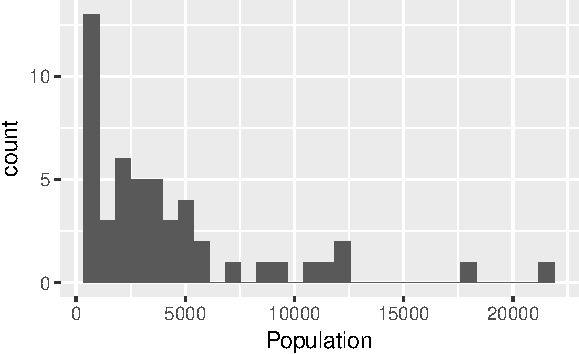
\includegraphics{pdaps_files/figure-latex/histogram-1.pdf}

Let's walk through the syntax there. In the first line, we call \texttt{ggplot()}, specifying the data frame to draw from, then in the \texttt{aes()} command (which stands for ``aesthetic'') we specify the variable to plot. If this were a bivariate analysis, here we would have also specified a \texttt{y} variable to put on the y-axis. If we had just stopped there, we would have a sad, empty plot. The \texttt{+} symbol indicates that we'll be adding something to the plot. \texttt{geom\_histogram()} is the command to overlay a histogram.

We'll only be looking at a few of the ggplot commands today. I recommend taking a look at the online package documentation at \url{http://docs.ggplot2.org} to see all of the many features available.

When you're just making graphs for yourself to explore the data, you don't need to worry about things like axis labels as long as you can comprehend what's going on. But when you prepare graphs for others to read (including those of us grading your problem sets!) you need to include an informative title and axis labels. To that end, use the \texttt{xlab()}, \texttt{ylab()}, and \texttt{ggtitle()} commands.

\begin{Shaded}
\begin{Highlighting}[]
\KeywordTok{ggplot}\NormalTok{(state\_data, }\KeywordTok{aes}\NormalTok{(}\DataTypeTok{x =}\NormalTok{ Population)) }\OperatorTok{+}
\StringTok{  }\KeywordTok{geom\_histogram}\NormalTok{() }\OperatorTok{+}
\StringTok{  }\KeywordTok{xlab}\NormalTok{(}\StringTok{"Population (thousands)"}\NormalTok{) }\OperatorTok{+}
\StringTok{  }\KeywordTok{ylab}\NormalTok{(}\StringTok{"Number of states"}\NormalTok{) }\OperatorTok{+}
\StringTok{  }\KeywordTok{ggtitle}\NormalTok{(}\StringTok{"Some states are big, but most are small"}\NormalTok{)}
\end{Highlighting}
\end{Shaded}

\begin{verbatim}
## `stat_bin()` using `bins = 30`. Pick better value with `binwidth`.
\end{verbatim}

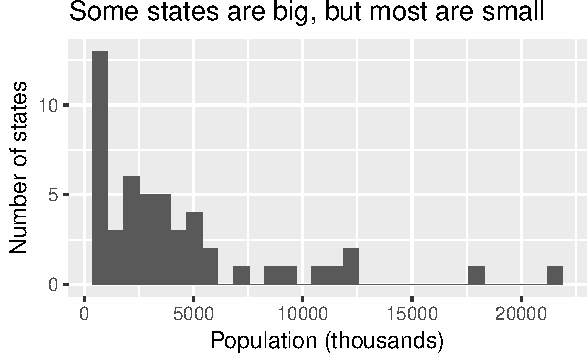
\includegraphics{pdaps_files/figure-latex/axis-labeling-1.pdf}

The density plot is a close relative of the histogram. It provides a smooth estimate of the probability density function of the data. Accordingly, the area under the density plot integrates to one. Depending on your purposes, this can make the y-axis of a density plot easier or (usually) harder to interpret than the count given by a histogram.

\begin{Shaded}
\begin{Highlighting}[]
\KeywordTok{ggplot}\NormalTok{(state\_data, }\KeywordTok{aes}\NormalTok{(}\DataTypeTok{x =}\NormalTok{ Population)) }\OperatorTok{+}
\StringTok{  }\KeywordTok{geom\_density}\NormalTok{()}
\end{Highlighting}
\end{Shaded}

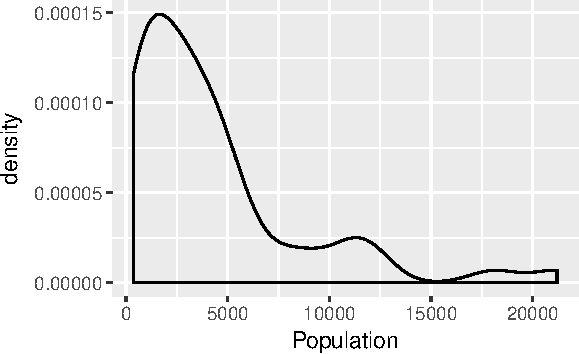
\includegraphics{pdaps_files/figure-latex/density-1.pdf}

The box plot is a common way to look at the distribution of a continuous variable across different levels of a categorical variable.

\begin{Shaded}
\begin{Highlighting}[]
\KeywordTok{ggplot}\NormalTok{(state\_data, }\KeywordTok{aes}\NormalTok{(}\DataTypeTok{x =}\NormalTok{ Region, }\DataTypeTok{y =}\NormalTok{ Population)) }\OperatorTok{+}
\StringTok{  }\KeywordTok{geom\_boxplot}\NormalTok{()}
\end{Highlighting}
\end{Shaded}

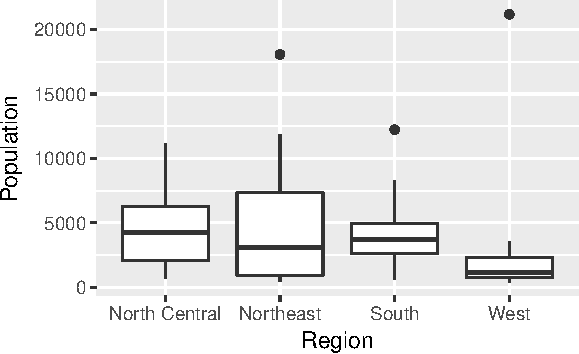
\includegraphics{pdaps_files/figure-latex/boxplot-1.pdf}

A box plot consists of the following components:

\begin{itemize}
\tightlist
\item
  Center line: median of the data
\item
  Bottom of box: 25th percentile
\item
  Top of box: 75th percentile
\item
  Lower ``whisker'': range of observations no more than 1.5 IQR (height of box) below the 25th percentile
\item
  Upper ``whisker'': range of observations no more than 1.5 IQR above the 75th percentile
\item
  Plotted points: any data lying outside the whiskers
\end{itemize}

If you want to skip the summary and plot the full distribution of a variable across categories, you can use a violin plot.

\begin{Shaded}
\begin{Highlighting}[]
\KeywordTok{ggplot}\NormalTok{(state\_data, }\KeywordTok{aes}\NormalTok{(}\DataTypeTok{x =}\NormalTok{ Region, }\DataTypeTok{y =}\NormalTok{ Population)) }\OperatorTok{+}
\StringTok{  }\KeywordTok{geom\_violin}\NormalTok{()}
\end{Highlighting}
\end{Shaded}

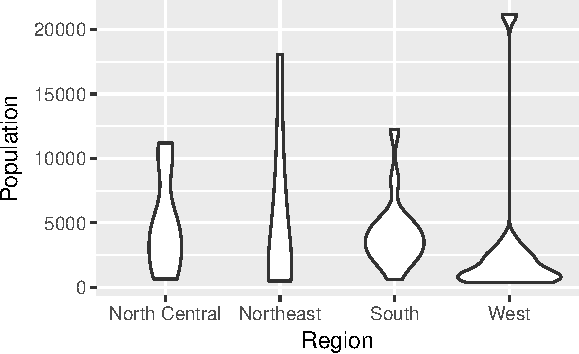
\includegraphics{pdaps_files/figure-latex/violin-1.pdf}

Technically, violin plots convey more information than box plots since they show the full distribution. However, readers aren't as likely to be familiar with a violin plot. It's harder to spot immediately where the median is (though you could add that to the plot if you wanted). Plus, violin plots look goofy with outliers---see the ``West'' column above---whereas box plots handle them easily.

For visualizing relationships between continuous variables, nothing beats the scatterplot.

\begin{Shaded}
\begin{Highlighting}[]
\KeywordTok{ggplot}\NormalTok{(state\_data, }\KeywordTok{aes}\NormalTok{(}\DataTypeTok{x =}\NormalTok{ Illiteracy, }\DataTypeTok{y =}\NormalTok{ LifeExp)) }\OperatorTok{+}
\StringTok{  }\KeywordTok{geom\_point}\NormalTok{()}
\end{Highlighting}
\end{Shaded}

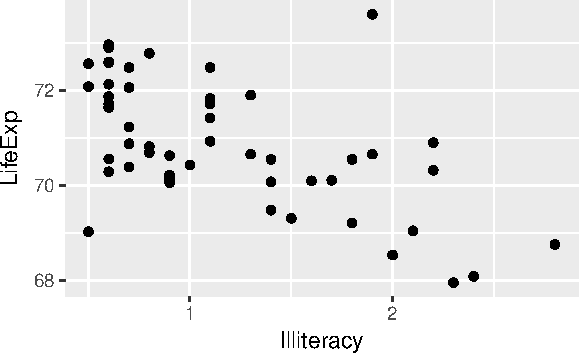
\includegraphics{pdaps_files/figure-latex/scatter-1.pdf}

When you're plotting states or countries, a hip thing to do is plot abbreviated names instead of points. To do that, you can use \texttt{geom\_text()} instead of \texttt{geom\_point()}, supplying an additional aesthetic argument telling ggplot where to draw the labels from.

\begin{Shaded}
\begin{Highlighting}[]
\KeywordTok{ggplot}\NormalTok{(state\_data, }\KeywordTok{aes}\NormalTok{(}\DataTypeTok{x =}\NormalTok{ Illiteracy, }\DataTypeTok{y =}\NormalTok{ LifeExp)) }\OperatorTok{+}
\StringTok{  }\KeywordTok{geom\_text}\NormalTok{(}\KeywordTok{aes}\NormalTok{(}\DataTypeTok{label =}\NormalTok{ Abbrev))}
\end{Highlighting}
\end{Shaded}

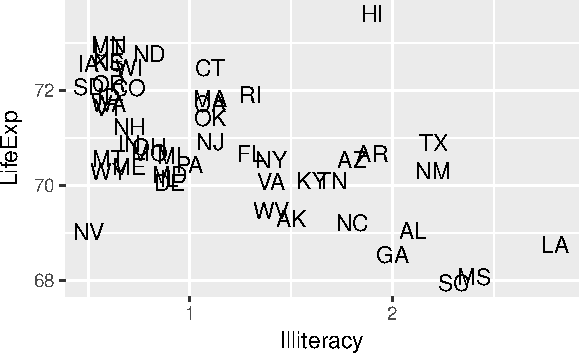
\includegraphics{pdaps_files/figure-latex/scatter-text-1.pdf}

Maybe it's overwhelming to look at all that raw data and you just want a summary. For example, maybe you want an estimate of expected \texttt{LifeExp} for each value of \texttt{Illiteracy}. This is called the \emph{conditional expectation} and will be the subject of much of the rest of the course. For now, just now that you can calculate a smoothed conditional expectation via \texttt{geom\_smooth()}.

\begin{Shaded}
\begin{Highlighting}[]
\KeywordTok{ggplot}\NormalTok{(state\_data, }\KeywordTok{aes}\NormalTok{(}\DataTypeTok{x =}\NormalTok{ Illiteracy, }\DataTypeTok{y =}\NormalTok{ LifeExp)) }\OperatorTok{+}
\StringTok{  }\KeywordTok{geom\_smooth}\NormalTok{()}
\end{Highlighting}
\end{Shaded}

\begin{verbatim}
## `geom_smooth()` using method = 'loess' and formula 'y ~ x'
\end{verbatim}

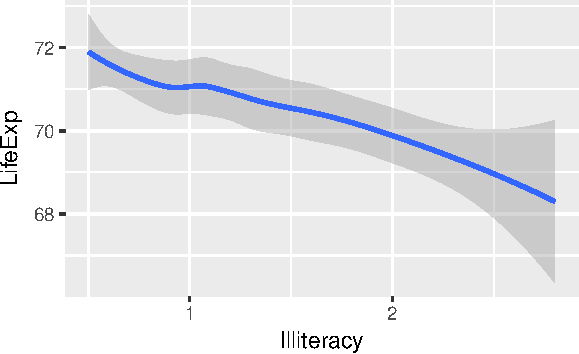
\includegraphics{pdaps_files/figure-latex/smooth-1.pdf}

And if you're the kind of overachiever who likes to have the raw data \emph{and} the summary, you can do it. Just add them both to the \texttt{ggplot()} call.

\begin{Shaded}
\begin{Highlighting}[]
\KeywordTok{ggplot}\NormalTok{(state\_data, }\KeywordTok{aes}\NormalTok{(}\DataTypeTok{x =}\NormalTok{ Illiteracy, }\DataTypeTok{y =}\NormalTok{ LifeExp)) }\OperatorTok{+}
\StringTok{  }\KeywordTok{geom\_smooth}\NormalTok{() }\OperatorTok{+}
\StringTok{  }\KeywordTok{geom\_point}\NormalTok{()}
\end{Highlighting}
\end{Shaded}

\begin{verbatim}
## `geom_smooth()` using method = 'loess' and formula 'y ~ x'
\end{verbatim}

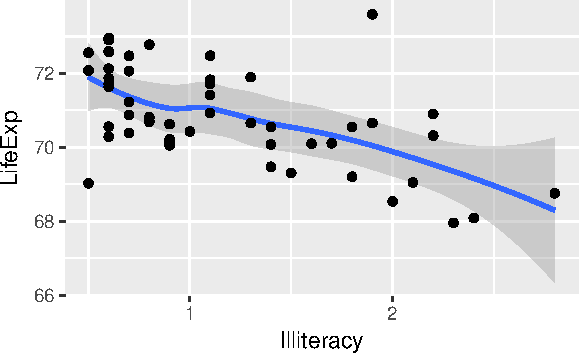
\includegraphics{pdaps_files/figure-latex/combine-1.pdf}

\hypertarget{saving-plots}{%
\section{Saving Plots}\label{saving-plots}}

When you're writing in R Markdown, the plots go straight into your document without much fuss. Odds are, your dissertation will contain plots but won't be written in R Markdown, which means you'll need to learn how to save them.

It's pretty simple:

\begin{enumerate}
\def\labelenumi{\arabic{enumi}.}
\tightlist
\item
  Assign your \texttt{ggplot()} call to a variable.
\item
  Pass that variable to the \texttt{ggsave()} function.
\end{enumerate}

\begin{Shaded}
\begin{Highlighting}[]
\NormalTok{pop\_hist \textless{}{-}}\StringTok{ }\KeywordTok{ggplot}\NormalTok{(state\_data, }\KeywordTok{aes}\NormalTok{(}\DataTypeTok{x =}\NormalTok{ Population)) }\OperatorTok{+}
\StringTok{  }\KeywordTok{geom\_histogram}\NormalTok{()}

\KeywordTok{ggsave}\NormalTok{(}\DataTypeTok{filename =} \StringTok{"pop{-}hist.pdf"}\NormalTok{,}
       \DataTypeTok{plot =}\NormalTok{ pop\_hist,}
       \DataTypeTok{width =} \DecValTok{6}\NormalTok{,}
       \DataTypeTok{height =} \DecValTok{3}\NormalTok{)}
\end{Highlighting}
\end{Shaded}

If you want plot types other than PDF, just set a different extension. See \texttt{?ggsave} for the possibilities.

\hypertarget{faceting}{%
\section{Faceting}\label{faceting}}

Suppose you want to split the data into subgroups, as defined by some variable in the data (e.g., the region states are in), and make the same plot for each subgroup. ggplot's \emph{faceting} functions, \texttt{facet\_wrap()} and \texttt{facet\_grid()}, make this easy.

To split up plots according to a single grouping variable, use \texttt{facet\_wrap()}. This uses R's \emph{formula} syntax, defined by the tilde \texttt{\textasciitilde{}}, which you'll become well acquainted with once we start running regressions.

\begin{Shaded}
\begin{Highlighting}[]
\KeywordTok{ggplot}\NormalTok{(state\_data, }\KeywordTok{aes}\NormalTok{(}\DataTypeTok{x =}\NormalTok{ Population)) }\OperatorTok{+}
\StringTok{  }\KeywordTok{geom\_histogram}\NormalTok{() }\OperatorTok{+}
\StringTok{  }\KeywordTok{facet\_wrap}\NormalTok{(}\OperatorTok{\textasciitilde{}}\StringTok{ }\NormalTok{Region)}
\end{Highlighting}
\end{Shaded}

\begin{verbatim}
## `stat_bin()` using `bins = 30`. Pick better value with `binwidth`.
\end{verbatim}

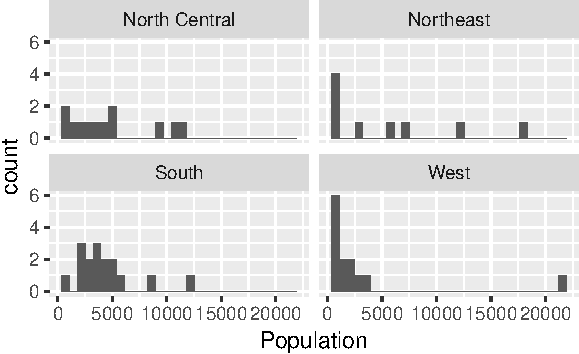
\includegraphics{pdaps_files/figure-latex/facet-wrap-1.pdf}

If you don't like the default arrangement, use the \texttt{ncol} argument.

\begin{Shaded}
\begin{Highlighting}[]
\KeywordTok{ggplot}\NormalTok{(state\_data, }\KeywordTok{aes}\NormalTok{(}\DataTypeTok{x =}\NormalTok{ Population)) }\OperatorTok{+}
\StringTok{  }\KeywordTok{geom\_histogram}\NormalTok{() }\OperatorTok{+}
\StringTok{  }\KeywordTok{facet\_wrap}\NormalTok{(}\OperatorTok{\textasciitilde{}}\StringTok{ }\NormalTok{Region, }\DataTypeTok{ncol =} \DecValTok{1}\NormalTok{)}
\end{Highlighting}
\end{Shaded}

\begin{verbatim}
## `stat_bin()` using `bins = 30`. Pick better value with `binwidth`.
\end{verbatim}

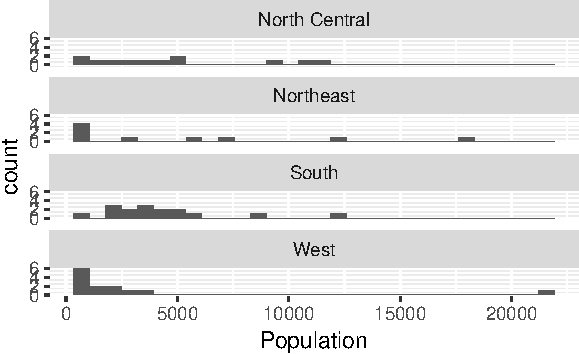
\includegraphics{pdaps_files/figure-latex/facet-wrap-ncol-1.pdf}

For two grouping variables, use \texttt{facet\_grid()}, putting variables on both sides of the formula.

\begin{Shaded}
\begin{Highlighting}[]
\KeywordTok{ggplot}\NormalTok{(state\_data, }\KeywordTok{aes}\NormalTok{(}\DataTypeTok{x =}\NormalTok{ Population)) }\OperatorTok{+}
\StringTok{  }\KeywordTok{geom\_histogram}\NormalTok{() }\OperatorTok{+}
\StringTok{  }\KeywordTok{facet\_grid}\NormalTok{(Region }\OperatorTok{\textasciitilde{}}\StringTok{ }\NormalTok{IncomeGroup)}
\end{Highlighting}
\end{Shaded}

\begin{verbatim}
## `stat_bin()` using `bins = 30`. Pick better value with `binwidth`.
\end{verbatim}

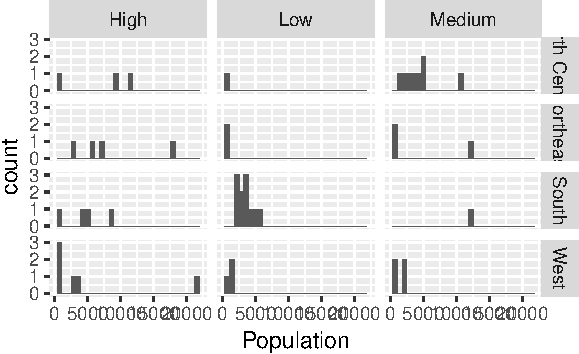
\includegraphics{pdaps_files/figure-latex/facet-grid-1.pdf}

\hypertarget{aesthetics}{%
\section{Aesthetics}\label{aesthetics}}

Faceting is one way to incorporate information about additional variables into what would otherwise be a plot of just one or two variables. Aesthetics---which alter the appearance of particular plot features depending on the value of a variable---provide another way to do that.

For example, when visualizing the relationship between statewide illiteracy and life expectancy, you might want larger states to get more visual weight. You can set the \texttt{size} aesthetic of the \texttt{point} geometry to vary according to the state's population.

\begin{Shaded}
\begin{Highlighting}[]
\KeywordTok{ggplot}\NormalTok{(state\_data, }\KeywordTok{aes}\NormalTok{(}\DataTypeTok{x =}\NormalTok{ Illiteracy, }\DataTypeTok{y =}\NormalTok{ LifeExp)) }\OperatorTok{+}
\StringTok{  }\KeywordTok{geom\_point}\NormalTok{(}\KeywordTok{aes}\NormalTok{(}\DataTypeTok{size =}\NormalTok{ Population))}
\end{Highlighting}
\end{Shaded}

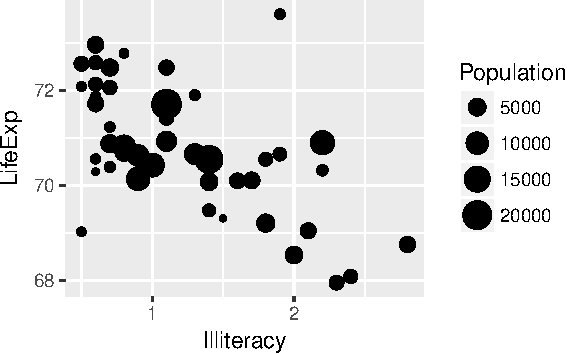
\includegraphics{pdaps_files/figure-latex/aes-size-1.pdf}

The \textbf{ggplot2} documentation lists the available aesthetics for each function. Another popular one is \texttt{colour}, which is great for on-screen display but not so much for the printed page. (And terrible for the colorblind!)

\begin{Shaded}
\begin{Highlighting}[]
\KeywordTok{ggplot}\NormalTok{(state\_data, }\KeywordTok{aes}\NormalTok{(}\DataTypeTok{x =}\NormalTok{ Illiteracy, }\DataTypeTok{y =}\NormalTok{ LifeExp)) }\OperatorTok{+}
\StringTok{  }\KeywordTok{geom\_point}\NormalTok{(}\KeywordTok{aes}\NormalTok{(}\DataTypeTok{colour =}\NormalTok{ Region))}
\end{Highlighting}
\end{Shaded}

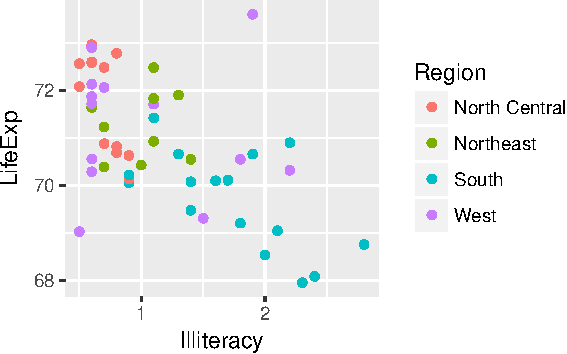
\includegraphics{pdaps_files/figure-latex/aes-colour-1.pdf}

For line graphs or density plots, you can set the \texttt{linetype} to vary by category.

\begin{Shaded}
\begin{Highlighting}[]
\KeywordTok{ggplot}\NormalTok{(state\_data, }\KeywordTok{aes}\NormalTok{(}\DataTypeTok{x =}\NormalTok{ Population)) }\OperatorTok{+}
\StringTok{  }\KeywordTok{geom\_density}\NormalTok{(}\KeywordTok{aes}\NormalTok{(}\DataTypeTok{linetype =}\NormalTok{ IncomeGroup))}
\end{Highlighting}
\end{Shaded}

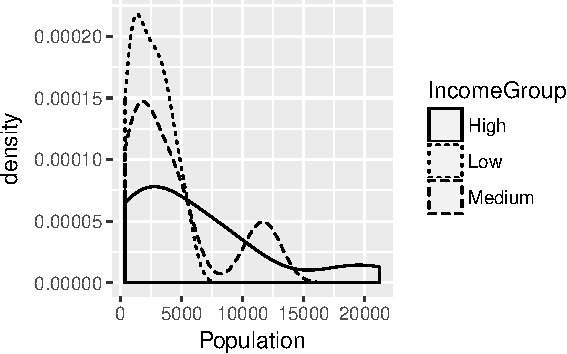
\includegraphics{pdaps_files/figure-latex/aes-linetype-1.pdf}

(I always find these incomprehensible with more than two lines, but maybe that's just me.) You can use multiple aesthetics together, and you can even combine aesthetics with faceting, as in the following example.

\begin{Shaded}
\begin{Highlighting}[]
\KeywordTok{ggplot}\NormalTok{(state\_data, }\KeywordTok{aes}\NormalTok{(}\DataTypeTok{x =}\NormalTok{ Illiteracy, }\DataTypeTok{y =}\NormalTok{ LifeExp)) }\OperatorTok{+}
\StringTok{  }\KeywordTok{geom\_smooth}\NormalTok{() }\OperatorTok{+}
\StringTok{  }\KeywordTok{geom\_text}\NormalTok{(}\KeywordTok{aes}\NormalTok{(}\DataTypeTok{label =}\NormalTok{ Abbrev, }\DataTypeTok{colour =}\NormalTok{ Region, }\DataTypeTok{size =}\NormalTok{ Population)) }\OperatorTok{+}
\StringTok{  }\KeywordTok{facet\_wrap}\NormalTok{(}\OperatorTok{\textasciitilde{}}\StringTok{ }\NormalTok{IncomeGroup)}
\end{Highlighting}
\end{Shaded}

\begin{verbatim}
## `geom_smooth()` using method = 'loess' and formula 'y ~ x'
\end{verbatim}

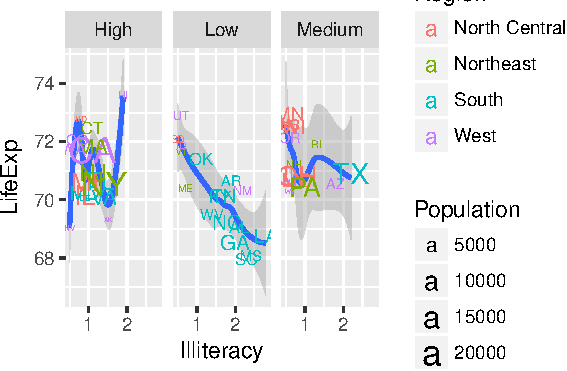
\includegraphics{pdaps_files/figure-latex/too-many-things-1.pdf}

But the fact that you \emph{can} do something doesn't mean you \emph{should}. That plot is so cluttered that it's hard to extract the relevant information from it. Data visualizations should communicate a clear message to viewers without overwhelming them. To do this well takes practice, patience, and maybe even a bit of taste.

\hypertarget{appendix-creating-the-example-data-1}{%
\section{Appendix: Creating the Example Data}\label{appendix-creating-the-example-data-1}}

The example data comes from data on U.S. states in 1977 that are included with base R. See \texttt{?state}.

\begin{Shaded}
\begin{Highlighting}[]
\KeywordTok{library}\NormalTok{(}\StringTok{"tidyverse"}\NormalTok{)}

\NormalTok{state\_data \textless{}{-}}\StringTok{ }\NormalTok{state.x77 }\OperatorTok{\%\textgreater{}\%}
\StringTok{  }\KeywordTok{as\_tibble}\NormalTok{() }\OperatorTok{\%\textgreater{}\%}
\StringTok{  }\KeywordTok{add\_column}\NormalTok{(}\DataTypeTok{State =} \KeywordTok{rownames}\NormalTok{(state.x77),}
             \DataTypeTok{Abbrev =}\NormalTok{ state.abb,}
             \DataTypeTok{Region =}\NormalTok{ state.region,}
             \DataTypeTok{.before =} \DecValTok{1}\NormalTok{) }\OperatorTok{\%\textgreater{}\%}
\StringTok{  }\KeywordTok{rename}\NormalTok{(}\DataTypeTok{LifeExp =} \StringTok{\textasciigrave{}}\DataTypeTok{Life Exp}\StringTok{\textasciigrave{}}\NormalTok{,}
         \DataTypeTok{HSGrad =} \StringTok{\textasciigrave{}}\DataTypeTok{HS Grad}\StringTok{\textasciigrave{}}\NormalTok{) }\OperatorTok{\%\textgreater{}\%}
\StringTok{  }\KeywordTok{mutate}\NormalTok{(}\DataTypeTok{IncomeGroup =} \KeywordTok{cut}\NormalTok{(Income,}
                           \DataTypeTok{breaks =} \KeywordTok{quantile}\NormalTok{(Income,}
                                             \DataTypeTok{probs =} \KeywordTok{seq}\NormalTok{(}\DecValTok{0}\NormalTok{, }\DecValTok{1}\NormalTok{, }\DataTypeTok{by =} \DecValTok{1}\OperatorTok{/}\DecValTok{3}\NormalTok{)),}
                           \DataTypeTok{labels =} \KeywordTok{c}\NormalTok{(}\StringTok{"Low"}\NormalTok{, }\StringTok{"Medium"}\NormalTok{, }\StringTok{"High"}\NormalTok{),}
                           \DataTypeTok{include.lowest =} \OtherTok{TRUE}\NormalTok{))}

\KeywordTok{write\_csv}\NormalTok{(state\_data, }\DataTypeTok{path =} \StringTok{"state{-}data.csv"}\NormalTok{)}
\end{Highlighting}
\end{Shaded}

\hypertarget{bivariate}{%
\chapter{Bivariate Regression}\label{bivariate}}

\providecommand{\SSE}{\mathop{\rm SSE}\nolimits}
\providecommand{\RSS}{\mathop{\rm RSS}\nolimits}
\providecommand{\TSS}{\mathop{\rm TSS}\nolimits}
\providecommand{\Cov}{\mathop{\rm Cov}\nolimits}
\providecommand{\pderiv}[2]{\frac{\partial{}#1}{\partial{}#2}}

The goal of empirical social science is usually to learn about the relationships between variables in the social world. Our goals might be descriptive: were college graduates more likely to vote for Clinton in 2016? Or causal: does receiving more education make a person more liberal on average? Or predictive: what kinds of voters should Democrats target in 2020 to have the best chance of victory?

The linear model is one of the simplest ways to model relationships between variables. Ordinary least squares regression is one of the easiest and (often) best ways to estimate the parameters of the linear model. Consequently, a linear model estimated by OLS is the starting point for many analyses. We will start with the simplest case: regression on a single covariate.

\hypertarget{probability}{%
\section{Probability Refresher}\label{probability}}

Let \(Y\) be a random variable that takes values in the finite set \(\mathcal{Y}\) according to the probability mass function \(f_Y : \mathcal{Y} \to [0, 1]\). The \emph{expected value} (aka \emph{expectation}) of \(Y\) is the weighted average of each value in \(\mathcal{Y}\), where the weights are the corresponding probabilities:
\begin{equation}
E[Y] = \sum_{y \in \mathcal{Y}} y \: f_Y(y);
\end{equation}

For a continuous random variable \(Y\) on \(\mathbb{R}\) with probability density function \(f_Y\), the expected value is the analogous integral:
\begin{equation}
E[Y] = \int y \: f_Y(y) \, dy.
\end{equation}

Now suppose \((X, Y)\) is a pair of discrete random variables drawn according to the joint mass function \(f_{XY}\) on \(\mathcal{X} \times \mathcal{Y}\), with respective marginal mass functions \(f_X\) and \(f_Y\).\footnote{The marginal mass function, if you don't recall, is \(f_X(x) = \sum_{y \in \mathcal{Y}} f_{XY} (x, y)\). In the continuous case, the marginal density function is \(f_X(x) = \int f_{XY} (x, y) \, dy\).} Recall the formula for conditional probability,
\begin{equation}
\Pr(Y = y \,|\, X = x)
= \frac{\Pr(X = x, Y = y)}{\Pr(X = x)}
= \frac{f_{XY}(x, y)}{f_X(x)}.
\end{equation}
For each \(x \in \mathcal{X}\), we have the \emph{conditional mass function}
\begin{equation}
f_{Y|X}(y \,|\, x) = \frac{f_{XY}(x, y)}{f_X(x)}
\end{equation}
and corresponding \emph{conditional expectation}
\begin{equation}
E[Y | X = x]
= \sum_{y \in \mathcal{Y}} y \: f_{Y|X}(y \,|\, x).
\end{equation}

For continuous random variables, the conditional expectation is
\begin{equation}
E[Y | X = x]
= \int y \: f_{Y|X} (y \,|\, x) \, dy,
\end{equation}
where \(f_{Y|X}\) is the conditional density function.

A fun fact about conditional expectation that will prove useful later on is the \emph{law of iterated expectation}.
This rule tells us that the expected value of a random variable is equal to the weighted average of its conditional expectations.
More succinctly, the law of iterated expectation is
\[
E[Y] = E[ E[Y | X] ]
\]
The ``inner'' expectation there is taken with respect to the conditional distribution of \(Y\), treating \(X\) as fixed.
The ``outer'' expectation is with respect to the distribution of \(X\).
It's easy enough to prove the law of iterated expectation in the finite case, where we have
\[
\begin{aligned}
E[ E[Y | X] ]
&= \sum_{x \in \mathcal{X}} E[Y | X = x] \Pr(X = x) \\
&= \sum_{x \in \mathcal{X}} \left( \sum_{y \in \mathcal{Y}} y \Pr(Y = y \,|\, X = x) \right) \Pr(X = x) \\
&= \sum_{x \in \mathcal{X}} \sum_{y \in \mathcal{Y}} y \Pr(X = x, Y = y) \\
&= \sum_{y \in \mathcal{Y}} y \left( \sum_{x \in \mathcal{X}} \Pr(X = x, Y = y) \right) \\
&= \sum_{y \in \mathcal{Y}} y \Pr(Y = y) \\
&= E[Y].
\end{aligned}
\]

The \emph{variance} of a random variable \(Y\) is
\begin{equation}
V[Y] = E[(Y - E[Y])^2].
\end{equation}
Given a sample \(Y_1, \ldots, Y_N\) of observations of \(Y\), we usually estimate \(V[Y]\) with the \emph{sample variance}
\begin{equation}
S_Y^2 = \frac{1}{N-1} \sum_n (Y_n - \bar{Y})^2,
\end{equation}
where \(\bar{Y}\) is the sample mean and \(\sum_n\) denotes summation from \(n = 1\) to \(N\).

Similarly (in fact a generalization of the above), the \emph{covariance} between random variables \(X\) and \(Y\) is
\[
\mathop{\rm Cov}\nolimits[X, Y] = E[(X - E[X]) (Y - E[Y])],
\]
which we estimate with the \emph{sample covariance}
\begin{equation}
S_{XY} = \frac{1}{N-1} \sum_n (X_n - \bar{X}) (Y_n - \bar{Y}).
\end{equation}
A fun fact about the sample covariance is that
\begin{align}
S_{XY}
&= \frac{1}{N-1} \sum_n (X_n - \bar{X}) (Y_n - \bar{Y}) \\
&= \frac{1}{N-1} \left[ \sum_n X_n (Y_n - \bar{Y}) + \sum_n \bar{X} (Y_n - \bar{Y}) \right] \\
&= \frac{1}{N-1} \left[ \sum_n X_n (Y_n - \bar{Y}) + \bar{X} \sum_n (Y_n - \bar{Y}) \right] \\
&= \frac{1}{N-1} \sum_n X_n (Y_n - \bar{Y}).
\end{align}
If we had split up the second term instead of the first, we would see that
\[
S_{XY} = \frac{1}{N-1} \sum_n Y_n (X_n - \bar{X})
\]
as well.

Since the (sample) variance is a special case of the (sample) covariance, by the same token we have
\begin{equation}
S_Y^2 = \frac{1}{N-1} \sum_n Y_n (Y_n - \bar{Y}).
\end{equation}

\hypertarget{the-linear-model}{%
\section{The Linear Model}\label{the-linear-model}}

Suppose we observe a sequence of \(N\) draws from \(f_{XY}\), denoted \((X_1, Y_1), (X_2, Y_2), \ldots, (X_N, Y_N)\), or \(\{(X_n, Y_n)\}_{n=1}^N\) for short. What can we learn about the relationship between \(X\) and \(Y\) from this sample of data?

If we were really ambitious, we could try to estimate the shape of the full joint distribution, \(f_{XY}\). The joint distribution encodes everything there is to know about the relationship between the two variables, so it would be pretty useful to know. But except in the most trivial cases, it would be infeasible to estimate \(f_{XY}\) precisely. If \(X\) or \(Y\) can take on more than a few values, estimating the joint distribution would require an amount of data that we're unlikely to have.\footnote{This problem only gets worse as we move from bivariate into multivariate analysis, a phenomenon called the \emph{curse of dimensionality}.}

The first way we simplify our estimation task is to set our sights lower. Let \(Y\) be the \emph{response} or the \emph{dependent variable}---i.e., the thing we want to explain. We call \(X\) the \emph{covariate} or the \emph{independent variable}. Instead of estimating the full joint distribution, we're just going to try to learn the conditional expectation, \(E[Y \,|\, X]\). In other words, for each potential value of the covariate, what is the expected value of the response? This will allow us to answer questions like whether greater values of \(X\) are associated with greater values of \(Y\).

Two important things about the estimation of conditional expectations before we go any further.

\begin{enumerate}
\def\labelenumi{\arabic{enumi}.}
\item
  Statements about conditional expectations are not causal. If \(Y\) is rain and \(X\) is umbrella sales, we know \(E[Y | X]\) increases with \(X\), but that doesn't mean umbrella sales make it rain.

  We will spend some time in the latter part of the course on how to move from conditional expectations to causality. Then, in Stat III, you will learn about causal inference in excruciating detail.
\item
  The conditional expectation doesn't give you everything you'd want to know about the relationship between variables.

  As a hypothetical example, suppose I told you that taking a particular drug made people happier on average. In other words, \(E[\text{Happiness} \,|\, \text{Drug}] > E[\text{Happiness} \,|\, \text{No Drug}]\). Sounds great! Then imagine the dose-response graph looked like this:

\begin{verbatim}
## Warning: `data_frame()` is deprecated as of tibble 1.1.0.
## Please use `tibble()` instead.
## This warning is displayed once every 8 hours.
## Call `lifecycle::last_warnings()` to see where this warning was generated.
\end{verbatim}

  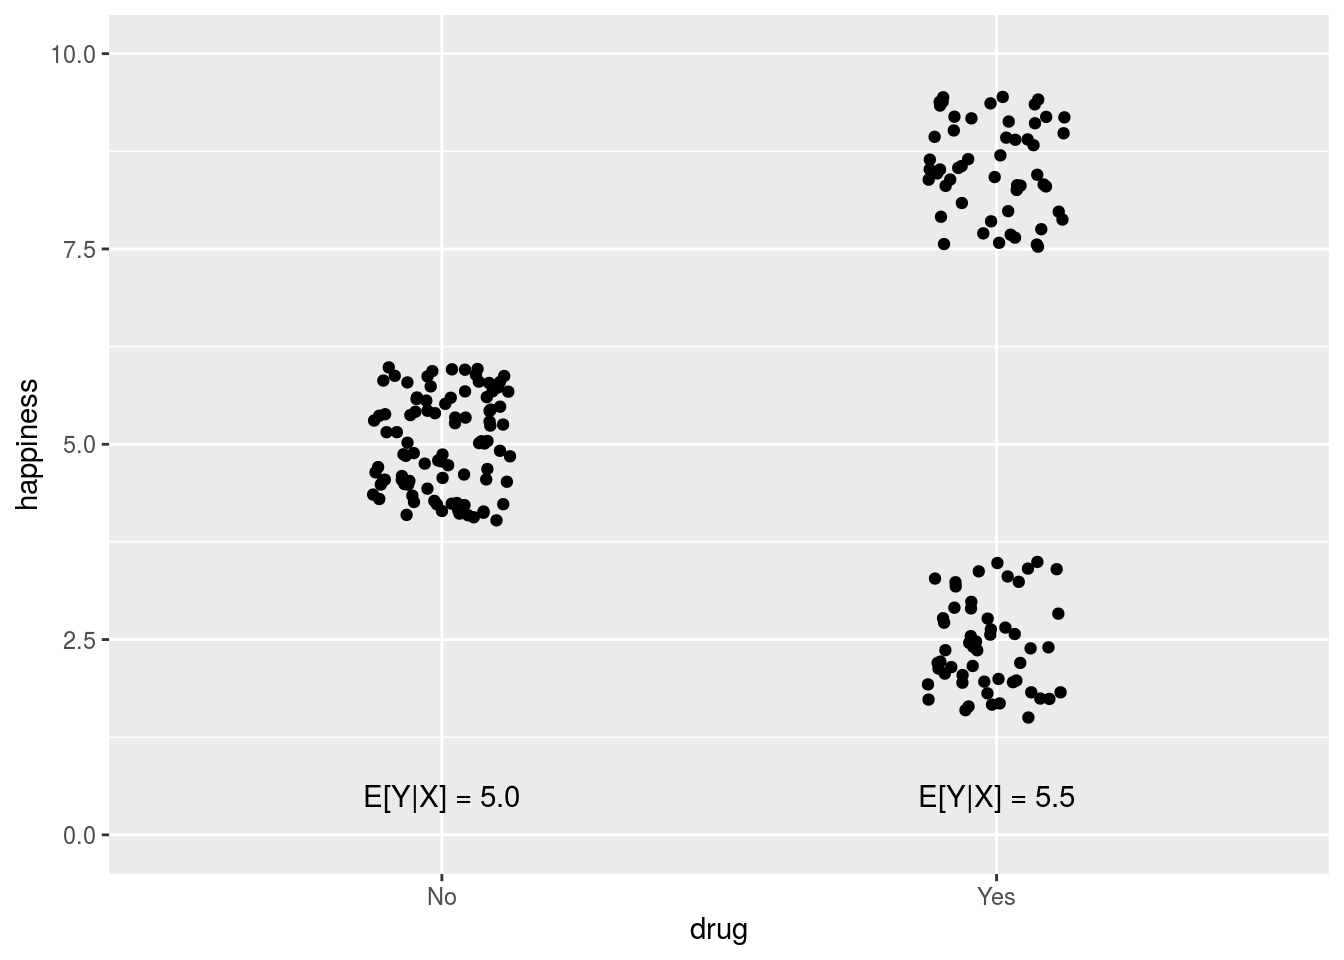
\includegraphics{pdaps_files/figure-latex/happiness-drug-1.pdf}

  The fact that expected happiness rises by half a point doesn't quite tell the whole story.
\end{enumerate}

In spite of these caveats, conditional expectation is a really useful tool for summarizing the relationship between variables.

If \(X\) takes on sufficiently few values (and we have enough data), we don't need to model the conditional expectation function. We can just directly estimate \(E[Y | X = x]\) for each \(x \in \mathcal{X}\). The graph above, where there are just two values of \(X\), is one example.

But if \(X\) is continuous, or even if it is discrete with many values, estimating \(E[Y | X]\) for each distinct value is infeasible. In this case, we need to \emph{model} the relationship. The very simplest choice---and thus the default for social scientists---is to model the conditional expectation of \(Y\) as a linear function of \(X\):
\begin{equation}
E[Y \,|\, X] = \alpha + \beta X.
\end{equation}
In this formulation, \(\alpha\) and \(\beta\) are the parameters to be estimated from sample data. We call \(\alpha\) and \(\beta\) ``coefficients,'' with \(\alpha\) the ``intercept'' and \(\beta\) the ``slope.'' Regardless of how many different values \(X\) might take on, we only need to estimate two parameters of the linear model.

Exercise your judgment before using a linear model. Ask yourself, is a linear conditional expectation function at least minimally plausible? Not perfect---just a reasonable approximation. If \(X\) is years of education and \(Y\) is annual income, the answer is probably yes (depending on the population!). But if \(X\) is hour of the day (0--24) and \(Y\) is the amount of traffic on I-65, probably not.

To obtain the linear conditional expectation, we usually assume the following model of the response variable:
\begin{equation}
Y_n = \alpha + \beta X_n + \epsilon_n,
\end{equation}
where \(\epsilon_n\) is ``white noise'' error with the property
\begin{equation}
E[\epsilon_n \,|\, X_1, \ldots X_N] = 0.
\end{equation}
You can think of \(\epsilon_n\) as the summation of everything besides the covariate \(X_n\) that affects the response \(Y_n\). The assumption that \(E[\epsilon_n \,|\, X_1, \ldots, X_N] = 0\) implies that these external factors are uncorrelated with the covariate. This is not a trivial technical condition that you can ignore---it is a substantive statement about the variables in your model. It requires justification, and it is difficult to justify.

For now we will proceed assuming that our data satisfy the above conditions. Later in the course, we will talk about how to proceed when \(E[\epsilon_n \,|\, X_1, \ldots, X_N] \neq 0\), and you will learn much more about such strategies in Stat III.

\hypertarget{least-squares}{%
\section{Least Squares}\label{least-squares}}

To estimate the parameters of the linear model, we will rely on a mathematically convenient method called \emph{least squares}. We will see that this method not only is convenient, but also has nice statistical properties.

Given a parameter estimate \((\hat{\alpha}, \hat{\beta})\), define the \emph{residual} of the \(n\)'th observation as the difference between the true and predicted values:
\begin{equation}
e_n(\hat{\alpha}, \hat{\beta}) = Y_n - \hat{\alpha} - \hat{\beta} X_n.
\end{equation}
The residual is directional. The residual is positive when the regression line falls below the observation, and vice versa when it is negative.

We would like the regression line to lie close to the data---i.e., for the residuals to be small in magnitude. ``Close'' can mean many things, so we need to be a bit more specific to derive an estimator. The usual one, \emph{ordinary least squares}, is chosen to minimize the sum of squared errors,
\[
\mathop{\rm SSE}\nolimits(\hat{\alpha}, \hat{\beta}) = \sum_n e_n(\hat{\alpha}, \hat{\beta})^2.
\]
(Throughout the rest of this chapter, I write \(\sum_n\) as shorthand for \(\sum_{n=1}^N\).) When we focus on squared error, we penalize a positive residual the same as a negative residual of the same size. Moreover, we penalize one big residual proportionally more than a few small ones.

It is important to keep the linear model and ordinary least squares distinct in your mind. The linear model is a model of the data. Ordinary least squares is one estimator---one among many---of the parameters of the linear model. Assuming a linear model does not commit you to estimate it with OLS if you think another estimator is more appropriate. And using OLS does not necessarily commit you to the linear model, as we will discuss when we get to multiple regression.

To derive the OLS estimator, we will derive the conditions for minimization of the sum of squared errors. The SSE is a quadratic and therefore continuously differentiable function of the estimands, \(\hat{\alpha}\) and \(\hat{\beta}\). You will remember from calculus that, at any extreme point of a continuous function, all its partial derivatives equal zero. To derive necessary conditions for minimization,\footnote{In fact, since the SSE function is strictly convex, these conditions are sufficient for global minimization.} we can take the derivatives of the SSE and set them to equal zero.

The derivative with respect to the intercept is
\[
\frac{\partial{}\mathop{\rm SSE}\nolimits(\hat{\alpha}, \hat{\beta})}{\partial{}\hat{\alpha}}
= -2 \sum_n (Y_n - \hat{\alpha} - \hat{\beta} X_n).
\]
Setting this to equal zero gives
\[
\hat{\alpha}
= \frac{1}{N} \sum_n (Y_n - \hat{\beta} X_n)
= \bar{Y} - \hat{\beta} \bar{X}.
\]
This gives us one important property of OLS: the regression line estimated by OLS always passes through \((\bar{X}, \bar{Y})\).

The derivative with respect to the slope is
\[
\frac{\partial{}\mathop{\rm SSE}\nolimits(\hat{\alpha}, \hat{\beta})}{\partial{}\hat{\beta}}
= -2 \sum_n X_n (Y_n - \hat{\alpha} - \hat{\beta} X_n).
\]
Setting this equal to zero and substituting in the expression for \(\hat{\alpha}\) we derived above gives
\[
\sum_n X_n (Y_n - \bar{Y}) = \hat{\beta} \sum_n X_n (X_n - \bar{X}).
\]
As long as the sample variance of \(X\) is non-zero (i.e., \(X\) is not a constant), we can divide to solve for \(\hat{\beta}\):
\[
\hat{\beta}
= \frac{\sum_n X_n (Y_n - \bar{Y})}{\sum_n X_n (X_n - \bar{X})}
= \frac{S_{XY}}{S_X^2}.
\]

Combining these two results, we have the OLS estimators of the intercept and slope of the bivariate linear model. We write them as functions of \((X_1, \ldots, X_N, Y_1, \ldots, Y_N)\), or \((X, Y)\) for short,\footnote{This is a bit of an abuse of notation, since previously I used \(X\) and \(Y\) to refer to the random variables and now I'm using them to refer to vectors of sample data. Sorry.} to emphasize that an estimator is a statistic, which in turn is a function of sample data. We place the ``OLS'' subscript on them to emphasize that there are many estimators of these parameters, of which OLS is just one (good!) choice.
\[
\begin{aligned}
\hat{\alpha}_{\text{OLS}}(X, Y)
&= \bar{Y} - \frac{S_{XY}}{S_X^2} \bar{X}, \\
\hat{\beta}_{\text{OLS}}(X, Y)
&= \frac{S_{XY}}{S_X^2}. \\
\end{aligned}
\]

Regression is a convenient way to summarize the relationship between variables, but it is a complement to---not a substitute for---graphical analysis. The statistician Francis Anscombe found that OLS yields nearly identical regression lines for all four of the datasets in the following graph:

\begin{verbatim}
## Warning: `as_data_frame()` is deprecated as of tibble 2.0.0.
## Please use `as_tibble()` instead.
## The signature and semantics have changed, see `?as_tibble`.
## This warning is displayed once every 8 hours.
## Call `lifecycle::last_warnings()` to see where this warning was generated.
\end{verbatim}

\begin{verbatim}
## `geom_smooth()` using formula 'y ~ x'
\end{verbatim}

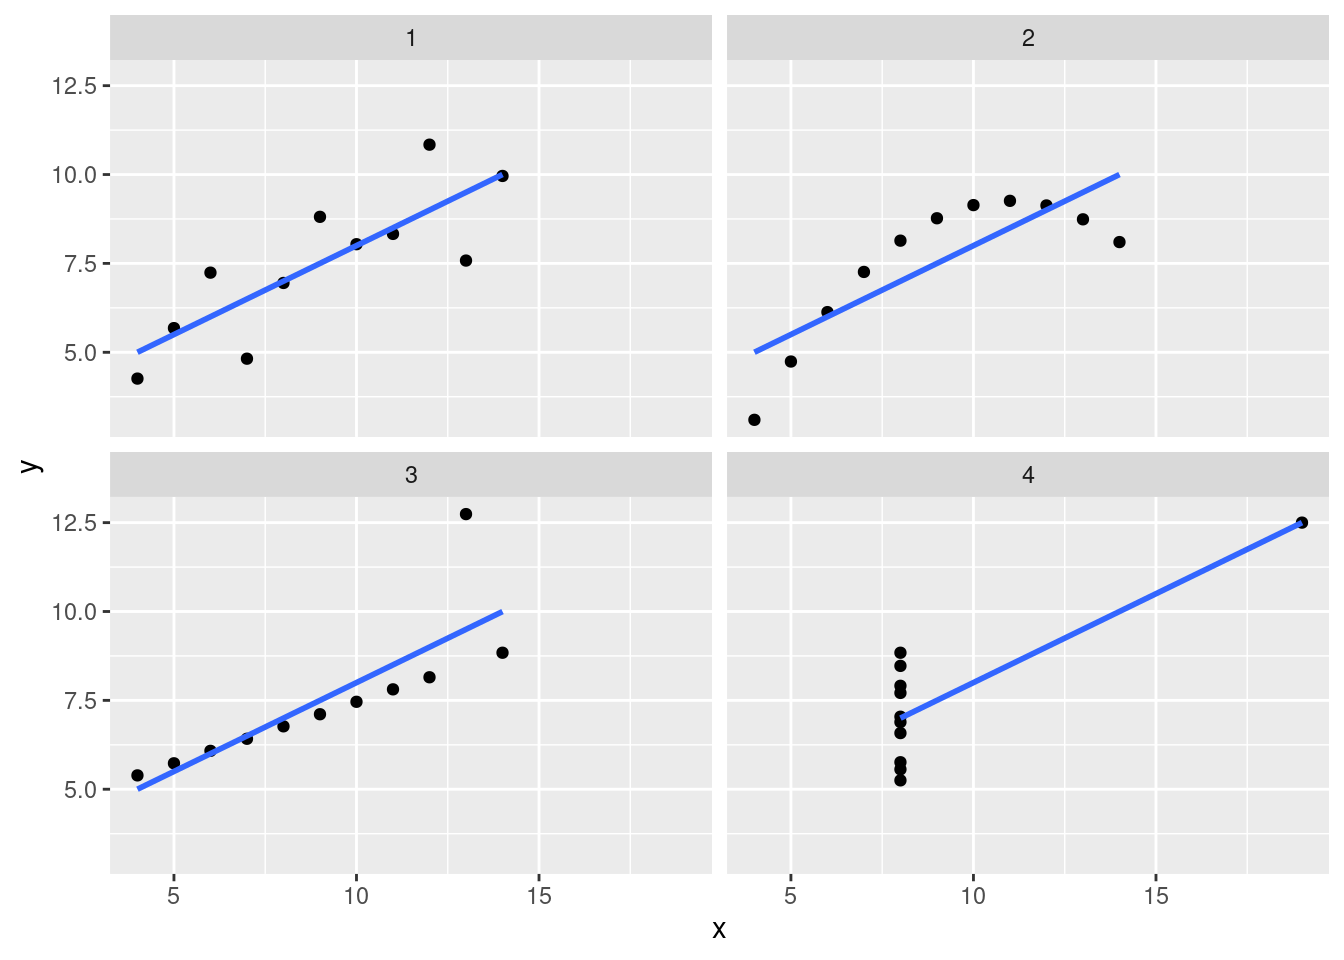
\includegraphics{pdaps_files/figure-latex/anscombe-1.pdf}

Unless your data all lie along a line, the regression line estimated by OLS will not predict the data perfectly. Let the \emph{residual sum of squares} be the squared error left over by OLS,
\[
\mathop{\rm RSS}\nolimits= \mathop{\rm SSE}\nolimits(\hat{\alpha}_{\text{OLS}}, \hat{\beta}_{\text{OLS}}),
\]
and let the \emph{total sum of squares} be the squared error that would result from a horizontal regression line through the mean of \(Y\),
\[
\mathop{\rm TSS}\nolimits= \mathop{\rm SSE}\nolimits(\bar{Y}, 0).
\]
The \(R^2\) statistic is the proportion of ``variance explained'' by \(X\), calculated as
\[
R^2 = 1 - \frac{\mathop{\rm RSS}\nolimits}{\mathop{\rm TSS}\nolimits}.
\]
If the regression line is flat, in which case \(\hat{\beta}_{\text{OLS}} = 0\) and \(\mathop{\rm RSS}\nolimits= \mathop{\rm TSS}\nolimits\), we have \(R^2= 0\). Conversely, if the regression line fits perfectly, in which case \(\mathop{\rm RSS}\nolimits= 0\), we have \(R^2 = 1\).

A statistic that is often more useful than \(R^2\) is the \emph{residual variance}. The residual variance is (almost) the sample variance of the regression residuals, calculated as
\[
\hat{\sigma}^2
= \frac{1}{N - 2} \sum_n e_n(\hat{\alpha}_{\text{OLS}}, \hat{\beta}_{\text{OLS}})^2
= \frac{\mathop{\rm RSS}\nolimits}{N - 2}
\]
Since bivariate regression uses two degrees of freedom (one for the intercept, one for the slope), we divide by \(N - 2\) instead of the usual \(N - 1\). The most useful quantity is \(\hat{\sigma}\), the square root of the residual variance. \(\hat{\sigma}\) is measured in the same units as \(Y\), and it is a measure of the spread of points around the regression line. If the residuals are roughly normally distributed, then we would expect roughly 95\% of the data to lie within \(\pm 2 \hat{\sigma}\) of the regression line.

\begin{verbatim}
## `geom_smooth()` using formula 'y ~ x'
\end{verbatim}

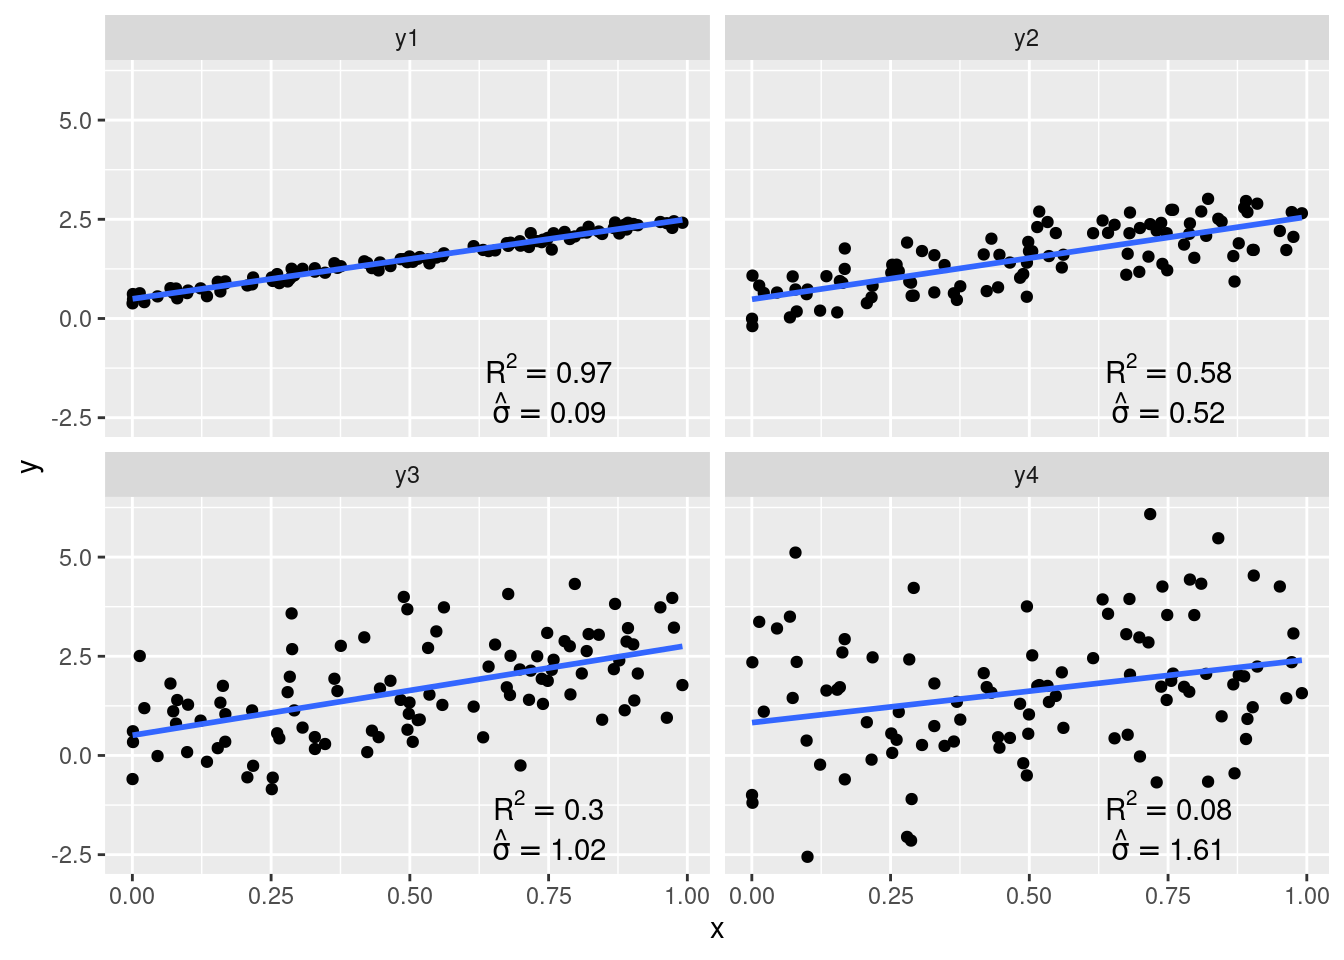
\includegraphics{pdaps_files/figure-latex/r2-examples-1.pdf}

\hypertarget{properties}{%
\section{Properties}\label{properties}}

We didn't use any fancy statistical theory to derive the OLS estimator. We just found the intercept and slope that minimize the sum of squared residuals. As it turns out, though, OLS indeed has some very nice statistical properties as an estimator of the linear model.

The first desirable property of OLS is that it is \emph{unbiased}. Recall that an estimator \(\hat{\theta}\) of the parameter \(\theta\) is unbiased if \(E[\hat{\theta}] = \theta\). This doesn't mean the estimator always gives us the right answer, just that on average it is not systematically biased upward or downward. In other words, if we could take many many samples and apply the estimator to each of them, the average would equal the true parameter.

We will begin by showing that the OLS estimator of the slope is unbiased; i.e., that \(E[\hat{\beta}_{\text{OLS}}(X, Y)] = \beta\). At first, we'll take the conditional expectation of the slope estimator, treating the covariates \((X_1, \ldots, X_N)\) as fixed.
\[
\begin{aligned}
E[\hat{\beta}_{\text{OLS}}(X, Y) \,|\, X]
&= E \left[ \left. \frac{S_{XY}}{S_X^2} \,\right|\, X \right] \\
&= E \left[ \left. \frac{\sum_n Y_n (X_n - \bar{X})}{\sum_n X_n (X_n - \bar{X})} \,\right|\, X \right] \\
&= \frac{\sum_n E[Y_n \,|\, X] (X_n - \bar{X})}{\sum_n X_n (X_n - \bar{X})} \\
&= \frac{\sum_n (\alpha + \beta X_n) (X_n - \bar{X})}{\sum_n X_n (X_n - \bar{X})} \\
&= \frac{\alpha \sum_n (X_n - \bar{X}) + \beta \sum_n X_n (X_n - \bar{X})}{\sum_n X_n (X_n - \bar{X})} \\
&= \frac{\beta \sum_n X_n (X_n - \bar{X})}{\sum_n X_n (X_n - \bar{X})} \\
&= \beta.
\end{aligned}
\]
It then follows from the \emph{law of iterated expectation}\footnote{For random variables \(A\) and \(B\), \(E[f(A, B)] = E_A[ E_B[f(A, B) \,|\, A] ] = E_B [ E_A[f(A, B) \,|\, B] ]\).} that
\[
E[\hat{\beta}_{\text{OLS}}(X, Y)] = \beta.
\]
Then, for the intercept, we have
\[
\begin{aligned}
E[\hat{\alpha}_{\text{OLS}}(X, Y) \,|\, X]
&= E [\bar{Y} - \hat{\beta}_{\text{OLS}}(X, Y) \bar{X} \,|\, X] \\
&= E [\bar{Y} \,|\, X] - E[\hat{\beta}_{\text{OLS}}(X, Y) \,|\, X] \bar{X} \\
&= E \left[ \left. \frac{1}{N} \sum_n Y_n \,\right|\, X \right] - \beta \bar{X} \\
&= E \left[ \left. \frac{1}{N} \sum_n (\alpha + \beta X_n + \epsilon_n) \,\right|\, X \right] - \beta \bar{X} \\
&= \frac{1}{N} \sum_n E[\alpha + \beta X_n + \epsilon_n \,|\, X] - \beta \bar{X} \\
&= \frac{1}{N} \sum_n \alpha + \frac{\beta}{N} \sum_n X_n + \frac{1}{N} \sum_n E[\epsilon_n \,|\, X] - \beta \bar{X} \\
&= \alpha + \beta \bar{X} - \beta \bar{X} \\
&= \alpha.
\end{aligned}
\]
As with the slope, this conditional expectation gives us the unconditional expectation we want:
\[
E[\hat{\alpha}_{\text{OLS}}(X, Y)] = \alpha.
\]

To sum up: as long as the crucial condition \(E[\epsilon_n \,|\, X_1, \ldots, X_N] = 0\) holds, then OLS is an unbiased estimator of the parameters of the linear model.

Another important property of OLS is that it is \emph{consistent}. Informally, this means that in sufficiently large samples, the OLS estimates \((\hat{\alpha}_{\text{OLS}}, \hat{\beta}_{\text{OLS}})\) are very likely to be close to the true parameter values \((\alpha, \beta)\). Another way to think of consistency is that, as \(N \to \infty\), the bias and variance of the OLS estimator both go to zero.\footnote{What I am describing here is \emph{mean square consistency}, which is stronger than the broadest definitions of consistency in statistical theory.}

Of course the bias ``goes to'' zero, since OLS is unbiased. The real trick to proving consistency is to show that the variance goes to zero. If you wanted to do that for the slope estimate, you'd derive an expression for
\[
V[\hat{\beta}_{\text{OLS}}]
=
E[(\hat{\beta}_{\text{OLS}} - E[\hat{\beta}_{\text{OLS}}])^2]
=
E[(\hat{\beta}_{\text{OLS}} - \beta)^2]
\]
and show that
\[
\lim_{N \to \infty} V[\hat{\beta}_{\text{OLS}}] = 0.
\]
This takes more algebra than we have time for, so I leave it as an exercise for the reader.

\hypertarget{appendix-regression-in-r}{%
\section{Appendix: Regression in R}\label{appendix-regression-in-r}}

We will be using the \textbf{tidyverse} package as always, the \textbf{car} package for the \texttt{Prestige} data, and the \textbf{broom} package for its convenient post-analysis functions.

\begin{Shaded}
\begin{Highlighting}[]
\KeywordTok{library}\NormalTok{(}\StringTok{"tidyverse"}\NormalTok{)}
\KeywordTok{library}\NormalTok{(}\StringTok{"car"}\NormalTok{)}
\KeywordTok{library}\NormalTok{(}\StringTok{"broom"}\NormalTok{)}
\end{Highlighting}
\end{Shaded}

Let's take a look at \texttt{Prestige}, which records basic information (including perceived prestige) for a variety of occupations.

\begin{Shaded}
\begin{Highlighting}[]
\KeywordTok{head}\NormalTok{(Prestige)}
\end{Highlighting}
\end{Shaded}

\begin{verbatim}
##                     education income women prestige census type
## gov.administrators      13.11  12351 11.16     68.8   1113 prof
## general.managers        12.26  25879  4.02     69.1   1130 prof
## accountants             12.77   9271 15.70     63.4   1171 prof
## purchasing.officers     11.42   8865  9.11     56.8   1175 prof
## chemists                14.62   8403 11.68     73.5   2111 prof
## physicists              15.64  11030  5.13     77.6   2113 prof
\end{verbatim}

Suppose we want to run a regression of prestige on education. We will use the \texttt{lm()} function, which stands for \emph{linear model}. This will employ the ``formula'' syntax that you previously saw when faceting in ggplot. The basic syntax of a formula is \texttt{response\ \textasciitilde{}\ covariate}, where \texttt{response} and \texttt{covariate} are the names of the variables in question. In this case, with \texttt{prestige} (note that the variable is lowercase, while the dataset is capitalized) as the response and education as the covariate:

\begin{Shaded}
\begin{Highlighting}[]
\KeywordTok{lm}\NormalTok{(prestige }\OperatorTok{\textasciitilde{}}\StringTok{ }\NormalTok{education, }\DataTypeTok{data =}\NormalTok{ Prestige)}
\end{Highlighting}
\end{Shaded}

\begin{verbatim}
## 
## Call:
## lm(formula = prestige ~ education, data = Prestige)
## 
## Coefficients:
## (Intercept)    education  
##     -10.732        5.361
\end{verbatim}

You'll notice that didn't give us very much. If you've previously used statistical programs like Stata, you might expect a ton of output at this point. It's all there in R too, but R has a different philosophy about models. R sees the fitted model as an object in its own right---like a data frame, a function, or anything else you load or create in R. Therefore, to analyze regression results in R, you will typically save the regression results to a variable.

Like any other variable, you'll want to give your regression results meaningful names. I typically call them \texttt{fit\_} to indicate a fitted model, followed by some memorable description.

\begin{Shaded}
\begin{Highlighting}[]
\NormalTok{fit\_educ \textless{}{-}}\StringTok{ }\KeywordTok{lm}\NormalTok{(prestige }\OperatorTok{\textasciitilde{}}\StringTok{ }\NormalTok{education, }\DataTypeTok{data =}\NormalTok{ Prestige)}
\end{Highlighting}
\end{Shaded}

When you do this, the output doesn't get printed. To see the default output, just run the variable name, just like you would to see the content of a data frame:

\begin{Shaded}
\begin{Highlighting}[]
\NormalTok{fit\_educ}
\end{Highlighting}
\end{Shaded}

\begin{verbatim}
## 
## Call:
## lm(formula = prestige ~ education, data = Prestige)
## 
## Coefficients:
## (Intercept)    education  
##     -10.732        5.361
\end{verbatim}

For a more detailed readout, use the \texttt{summary()} method:

\begin{Shaded}
\begin{Highlighting}[]
\KeywordTok{summary}\NormalTok{(fit\_educ)}
\end{Highlighting}
\end{Shaded}

\begin{verbatim}
## 
## Call:
## lm(formula = prestige ~ education, data = Prestige)
## 
## Residuals:
##      Min       1Q   Median       3Q      Max 
## -26.0397  -6.5228   0.6611   6.7430  18.1636 
## 
## Coefficients:
##             Estimate Std. Error t value Pr(>|t|)    
## (Intercept)  -10.732      3.677  -2.919  0.00434 ** 
## education      5.361      0.332  16.148  < 2e-16 ***
## ---
## Signif. codes:  0 '***' 0.001 '**' 0.01 '*' 0.05 '.' 0.1 ' ' 1
## 
## Residual standard error: 9.103 on 100 degrees of freedom
## Multiple R-squared:  0.7228, Adjusted R-squared:   0.72 
## F-statistic: 260.8 on 1 and 100 DF,  p-value: < 2.2e-16
\end{verbatim}

This prints out a whole boatload of information, including inferential statistics that we're going to wait until later in the course to discuss how to interpret:

\begin{itemize}
\tightlist
\item
  The model you ran
\item
  Basic statistics about the distribution of the residuals
\item
  For each coefficient:

  \begin{itemize}
  \tightlist
  \item
    Parameter estimate
  \item
    Standard error estimate
  \item
    Test statistic for a hypothesis test of equality with zero
  \item
    \(p\)-value associated with the test statistic
  \end{itemize}
\item
  \(\hat{\sigma}\) (called the ``residual standard error'', a term seemingly unique to R)
\item
  \(R^2\) and an ``adjusted'' variant that accounts for the number of variables in the model
\item
  \(F\) statistic, degrees of freedom, and associated \(p\)-value for a hypothesis test that every coefficient besides the intercept equals zero
\end{itemize}

Strangely, \texttt{summary()} doesn't give you the sample size. For that you must use \texttt{nobs()}:

\begin{Shaded}
\begin{Highlighting}[]
\KeywordTok{nobs}\NormalTok{(fit\_educ)}
\end{Highlighting}
\end{Shaded}

\begin{verbatim}
## [1] 102
\end{verbatim}

You can use a fitted model object to make predictions for new data. For example, let's make a basic data frame of education levels.

\begin{Shaded}
\begin{Highlighting}[]
\NormalTok{my\_data \textless{}{-}}\StringTok{ }\KeywordTok{data\_frame}\NormalTok{(}\DataTypeTok{education =} \DecValTok{8}\OperatorTok{:}\DecValTok{16}\NormalTok{)}
\NormalTok{my\_data}
\end{Highlighting}
\end{Shaded}

\begin{verbatim}
## # A tibble: 9 x 1
##   education
##       <int>
## 1         8
## 2         9
## 3        10
## 4        11
## 5        12
## 6        13
## 7        14
## 8        15
## 9        16
\end{verbatim}

To calculate the predicted level of prestige for each education level, use \texttt{predict()}:

\begin{Shaded}
\begin{Highlighting}[]
\KeywordTok{predict}\NormalTok{(fit\_educ, }\DataTypeTok{newdata =}\NormalTok{ my\_data)}
\end{Highlighting}
\end{Shaded}

\begin{verbatim}
##        1        2        3        4        5        6        7        8 
## 32.15504 37.51592 42.87680 48.23767 53.59855 58.95943 64.32031 69.68118 
##        9 
## 75.04206
\end{verbatim}

When using \texttt{predict()}, it is crucial that the \texttt{newdata} have the same column names as in the data used to fit the model.

You can also extract a confidence interval for each prediction:

\begin{Shaded}
\begin{Highlighting}[]
\KeywordTok{predict}\NormalTok{(fit\_educ,}
        \DataTypeTok{newdata =}\NormalTok{ my\_data,}
        \DataTypeTok{interval =} \StringTok{"confidence"}\NormalTok{,}
        \DataTypeTok{level =} \FloatTok{0.95}\NormalTok{)}
\end{Highlighting}
\end{Shaded}

\begin{verbatim}
##        fit      lwr      upr
## 1 32.15504 29.61530 34.69478
## 2 37.51592 35.39261 39.63922
## 3 42.87680 41.02363 44.72996
## 4 48.23767 46.44110 50.03425
## 5 53.59855 51.62654 55.57056
## 6 58.95943 56.63186 61.28700
## 7 64.32031 61.52495 67.11566
## 8 69.68118 66.35281 73.00956
## 9 75.04206 71.14209 78.94204
\end{verbatim}

One of the problems with \texttt{summary()} and \texttt{predict()} is that they return inconveniently shaped output. The output of \texttt{summary()} is particularly hard to deal with. The \textbf{broom} package provides three utilities to help get model output into shape. The first is \texttt{tidy()}, which makes a tidy data frame out of the regression coefficients and the associated inferential statistics:

\begin{Shaded}
\begin{Highlighting}[]
\KeywordTok{tidy}\NormalTok{(fit\_educ)}
\end{Highlighting}
\end{Shaded}

\begin{verbatim}
## # A tibble: 2 x 5
##   term        estimate std.error statistic  p.value
##   <chr>          <dbl>     <dbl>     <dbl>    <dbl>
## 1 (Intercept)   -10.7      3.68      -2.92 4.34e- 3
## 2 education       5.36     0.332     16.1  1.29e-29
\end{verbatim}

The second is \texttt{glance()}, which provides a one-row data frame containing overall model characteristics (e.g., \(R^2\) and \(\hat{\sigma}\)):

\begin{Shaded}
\begin{Highlighting}[]
\KeywordTok{glance}\NormalTok{(fit\_educ)}
\end{Highlighting}
\end{Shaded}

\begin{verbatim}
## # A tibble: 1 x 12
##   r.squared adj.r.squared sigma statistic  p.value    df logLik   AIC   BIC
##       <dbl>         <dbl> <dbl>     <dbl>    <dbl> <dbl>  <dbl> <dbl> <dbl>
## 1     0.723         0.720  9.10      261. 1.29e-29     1  -369.  744.  752.
## # ... with 3 more variables: deviance <dbl>, df.residual <int>, nobs <int>
\end{verbatim}

The third is \texttt{augment()}, which ``augments'' the original data---or new data you supply, as in \texttt{predict()}---with information from the model, such as predicted values.

\begin{Shaded}
\begin{Highlighting}[]
\CommentTok{\# Lots of output, so only printing first 10 rows}
\KeywordTok{head}\NormalTok{(}\KeywordTok{augment}\NormalTok{(fit\_educ), }\DecValTok{10}\NormalTok{)}
\end{Highlighting}
\end{Shaded}

\begin{verbatim}
## # A tibble: 10 x 9
##    .rownames  prestige education .fitted .resid .std.resid   .hat .sigma .cooksd
##    <chr>         <dbl>     <dbl>   <dbl>  <dbl>      <dbl>  <dbl>  <dbl>   <dbl>
##  1 gov.admin~     68.8      13.1    59.5   9.25      1.03  0.0173   9.10 9.24e-3
##  2 general.m~     69.1      12.3    55.0  14.1       1.56  0.0129   9.04 1.59e-2
##  3 accountan~     63.4      12.8    57.7   5.67      0.628 0.0153   9.13 3.06e-3
##  4 purchasin~     56.8      11.4    50.5   6.31      0.697 0.0104   9.13 2.56e-3
##  5 chemists       73.5      14.6    67.6   5.86      0.653 0.0298   9.13 6.56e-3
##  6 physicists     77.6      15.6    73.1   4.49      0.504 0.0418   9.14 5.53e-3
##  7 biologists     72.6      15.1    70.2   2.44      0.272 0.0350   9.15 1.35e-3
##  8 architects     78.1      15.4    72.0   6.06      0.679 0.0392   9.13 9.41e-3
##  9 civil.eng~     73.1      14.5    67.1   5.99      0.668 0.0288   9.13 6.62e-3
## 10 mining.en~     68.8      14.6    67.8   1.05      0.117 0.0301   9.15 2.12e-4
\end{verbatim}

\begin{Shaded}
\begin{Highlighting}[]
\KeywordTok{augment}\NormalTok{(fit\_educ,}
        \DataTypeTok{newdata =}\NormalTok{ my\_data)}
\end{Highlighting}
\end{Shaded}

\begin{verbatim}
## # A tibble: 9 x 2
##   education .fitted
##       <int>   <dbl>
## 1         8    32.2
## 2         9    37.5
## 3        10    42.9
## 4        11    48.2
## 5        12    53.6
## 6        13    59.0
## 7        14    64.3
## 8        15    69.7
## 9        16    75.0
\end{verbatim}

Notice that you get back more information for the data used to fit the model than for newly supplied data. The most important is \texttt{.fitted}, the predicted value. See \texttt{?augment.lm} for what all the various output represents.

One last note on plotting regression lines with ggplot. Use \texttt{geom\_smooth(method\ =\ "lm")}.

\begin{Shaded}
\begin{Highlighting}[]
\KeywordTok{ggplot}\NormalTok{(Prestige, }\KeywordTok{aes}\NormalTok{(}\DataTypeTok{x =}\NormalTok{ education, }\DataTypeTok{y =}\NormalTok{ prestige)) }\OperatorTok{+}
\StringTok{  }\KeywordTok{geom\_point}\NormalTok{() }\OperatorTok{+}
\StringTok{  }\KeywordTok{geom\_smooth}\NormalTok{(}\DataTypeTok{method =} \StringTok{"lm"}\NormalTok{)}
\end{Highlighting}
\end{Shaded}

\begin{verbatim}
## `geom_smooth()` using formula 'y ~ x'
\end{verbatim}

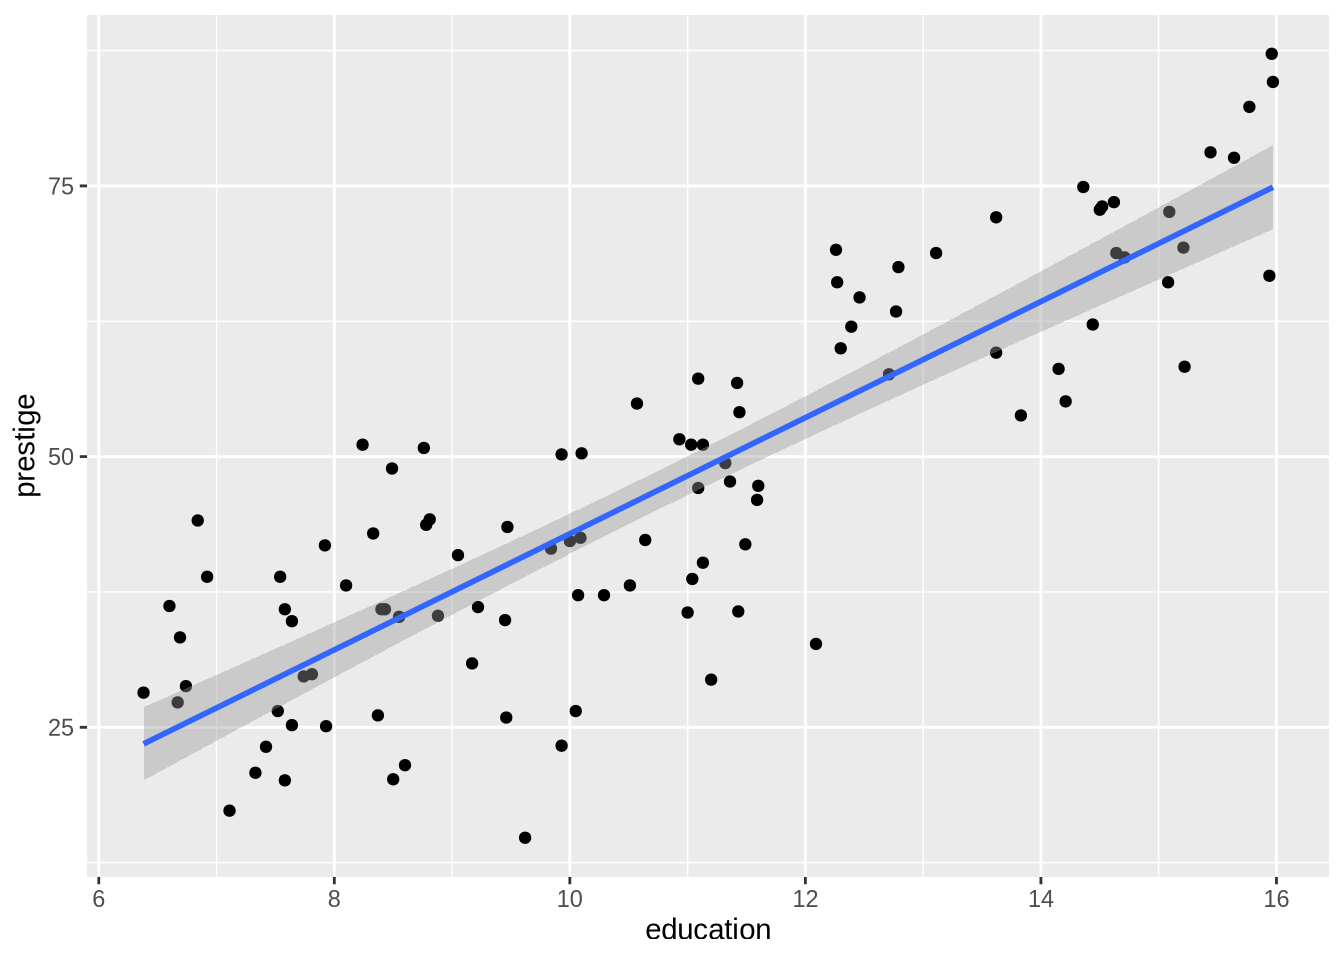
\includegraphics{pdaps_files/figure-latex/ggplot-lm-1.pdf}

To get rid of the confidence interval:

\begin{Shaded}
\begin{Highlighting}[]
\KeywordTok{ggplot}\NormalTok{(Prestige, }\KeywordTok{aes}\NormalTok{(}\DataTypeTok{x =}\NormalTok{ education, }\DataTypeTok{y =}\NormalTok{ prestige)) }\OperatorTok{+}
\StringTok{  }\KeywordTok{geom\_point}\NormalTok{() }\OperatorTok{+}
\StringTok{  }\KeywordTok{geom\_smooth}\NormalTok{(}\DataTypeTok{method =} \StringTok{"lm"}\NormalTok{, }\DataTypeTok{se =} \OtherTok{FALSE}\NormalTok{)}
\end{Highlighting}
\end{Shaded}

\begin{verbatim}
## `geom_smooth()` using formula 'y ~ x'
\end{verbatim}

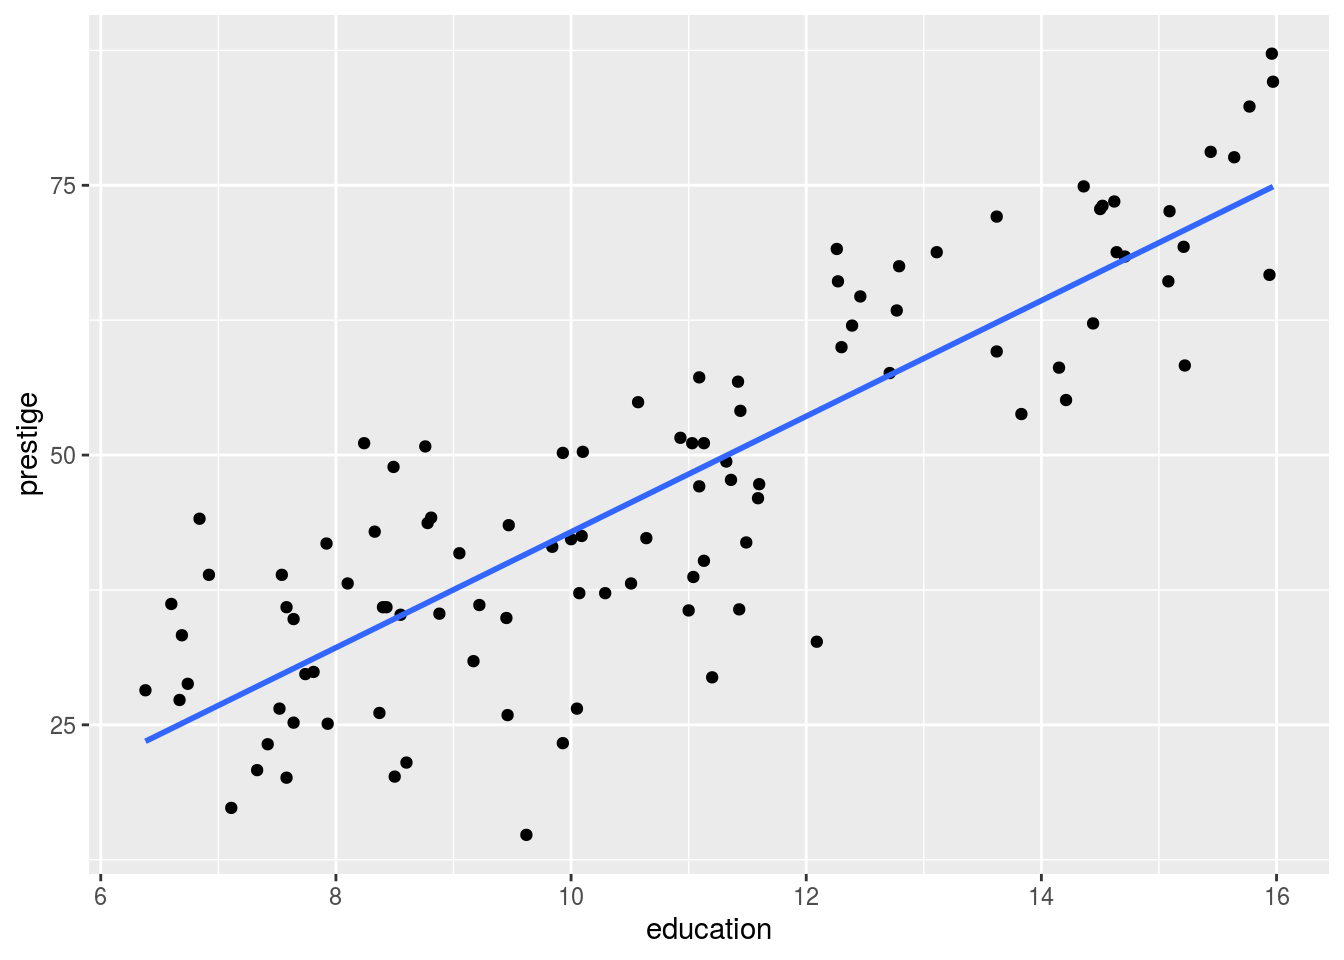
\includegraphics{pdaps_files/figure-latex/ggplot-lm-no-se-1.pdf}

\hypertarget{matrix}{%
\chapter{Matrix Algebra: A Crash Course}\label{matrix}}

\emph{Some material in this chapter is adapted from notes \href{https://hyeyoungyou.com}{Hye Young You} wrote for the math boot camp for the political science PhD program at Vanderbilt.}

Matrix algebra is an essential tool for understanding multivariate statistics. You are probably already familiar with matrices, at least informally. The data representations we have worked with so far---each row an observation, each column a variable---are formatted like matrices.

An introductory treatment of matrix algebra is a semester-long college course. We don't have that long, or even half that long. This chapter gives you the \emph{bare minimum} you need to understand to get up and running with the matrix algebra we need for OLS with multiple covariates. If you want to use advanced statistical methods in your research and haven't previously taken a matrix algebra or linear algebra course, I recommend taking some time this summer to catch up. For example, MIT has its undergraduate linear algebra course \href{https://ocw.mit.edu/courses/mathematics/18-06-linear-algebra-spring-2010/index.htm}{available online}, including video lectures.

\hypertarget{vector-operations}{%
\section{Vector Operations}\label{vector-operations}}

A \emph{vector} is an ordered array. To denote a vector \(v\) of \(k\) elements, we write \(\mathbf{v} = (v_1, v_2, \ldots, v_k)\), or sometimes
\[
\mathbf{v} = \begin{pmatrix} v_1 \\ v_2 \\ \vdots \\ v_k \end{pmatrix}.
\]
Notice the convention of using a lowercase bold letter to denote a vector. We will usually be dealing with vectors of real numbers. To denote the fact that \(\mathbf{v}\) is a vector of \(k\) real numbers, we write \(\mathbf{v} \in \mathbb{R}^k\).

A vector can be multiplied by a scalar \(c \in \mathbb{R}\), producing what you would expect:
\[
c \mathbf{v} = \begin{pmatrix} c v_1 \\ c v_2 \\ \vdots \\ c v_k \end{pmatrix}
\]
You can also add and subtract two vectors of the same length.\footnote{R will let you add and subtract vectors of different lengths, via a technique called ``recycling''. For example \texttt{c(1,\ 0)\ +\ c(1,\ 2,\ 3,\ 4)} will produce \texttt{c(2,\ 2,\ 4,\ 4)}. This is kosher in R, but not in mathematical derivations.}
\[
\begin{aligned}
\mathbf{u} + \mathbf{v} &= \begin{pmatrix}
  u_1 + v_1 \\ u_2 + v_2 \\ \vdots \\ u_k + v_k
\end{pmatrix}, \\
\mathbf{u} - \mathbf{v} &= \begin{pmatrix}
  u_1 - v_1 \\ u_2 - v_2 \\ \vdots \\ u_k - v_k
\end{pmatrix}.
\end{aligned}
\]

A special vector is the \emph{zero vector}, which contains---you guessed it---all zeroes. We write \(\mathbf{0}_k\) to denote the zero vector of length \(k\). When the length of the zero vector is clear from the context, we may just write \(\mathbf{0}\).

The last important vector operation is the \emph{dot product}. The dot product of \(\mathbf{u}\) and \(\mathbf{v}\), written \(\mathbf{u} \cdot \mathbf{v}\), is the sum of the products of the entries:
\[
\mathbf{u} \cdot \mathbf{v}
=
u_1 v_1 + u_2 v_2 + \cdots + u_k v_k
=
\sum_{m=1}^k u_m v_m.
\]

An important concept for regression analysis is the linear independence of a collection of vectors. Let \(\mathbf{v}_1, \ldots, \mathbf{v}_J\) be a collection of \(J\) vectors, each of length \(k\). We call \(\mathbf{u}\) a \emph{linear combination} of \(\mathbf{v}_1, \ldots, \mathbf{v}_J\) if there exist real numbers \(c_1, \ldots, c_J\) such that
\[
\mathbf{u} = c_1 \mathbf{v}_1 + \cdots + c_J \mathbf{v}_J = \sum_{j=1}^J c_j \mathbf{v}_j.
\]
A collection of vectors is \emph{linearly independent} if the only solution to
\[
c_1 \mathbf{v}_1 + \cdots + c_J \mathbf{v}_J = \mathbf{0}
\]
is \(c_1 = 0, \ldots, c_J = 0\). Otherwise, we call the vectors \emph{linearly dependent}. Some fun facts about linear independence:

\begin{itemize}
\item
  If any vector in \(\mathbf{v}_1, \ldots, \mathbf{v}_J\) is a linear combination of the others, then these vectors are linearly dependent.
\item
  A collection of \(J\) vectors of length \(k\) cannot be linearly independent if \(J > k\). In other words, given vectors of length \(k\), the most that can be linearly independent of each other is \(k\).
\item
  If any \(\mathbf{v}_j = \mathbf{0}\), then \(\mathbf{v}_1, \ldots, \mathbf{v}_J\) are linearly dependent. (Why?)
\end{itemize}

Examples:
\[
\begin{gathered}
\mathbf{v}_1 = \begin{pmatrix} 1 \\ 2 \\ 3 \end{pmatrix},
\mathbf{v}_2 = \begin{pmatrix} 2 \\ 4 \\ 6 \end{pmatrix}; \\
\mathbf{v}_1 = \begin{pmatrix} 1 \\ 2 \\ 3 \end{pmatrix},
\mathbf{v}_2 = \begin{pmatrix} 1 \\ 4 \\ 9 \end{pmatrix}; \\
\mathbf{v}_1 = \begin{pmatrix} 1 \\ 1 \\ 1 \end{pmatrix},
\mathbf{v}_2 = \begin{pmatrix} 0 \\ 1 \\ 0 \end{pmatrix},
\mathbf{v}_3 = \begin{pmatrix} 0 \\ 0 \\ 1 \end{pmatrix}; \\
\mathbf{v}_1 = \begin{pmatrix} 1 \\ 0 \\ 0 \end{pmatrix},
\mathbf{v}_2 = \begin{pmatrix} 14 \\ 12 \\ 0 \end{pmatrix},
\mathbf{v}_3 = \begin{pmatrix} 0 \\ -1 \\ 0 \end{pmatrix}.
\end{gathered}
\]

\hypertarget{matrix-operations}{%
\section{Matrix Operations}\label{matrix-operations}}

A matrix is a two-dimensional array of numbers, with entries in rows and columns. We call a matrix with \(n\) rows and \(m\) columns an \(n \times m\) matrix. For example, the following is a \(2 \times 3\) matrix:
\[
\mathbf{A}
=
\begin{bmatrix}
  99 & 73 & 2 \\
  13 & 40 & 41
\end{bmatrix}
\]
Notice the convention of using an uppercase bold letter to denote a matrix. Given a matrix \(\mathbf{A}\), we usually write \(a_{ij}\) to denote the entry in the \(i\)'th row and \(j\)'th column. In the above example, we have \(a_{13} = 2\).

You can think of a vector \(\mathbf{v} \in \mathbb{R}^k\) as a \(1 \times k\) \emph{row matrix} or as a \(k \times 1\) \emph{column matrix}. Throughout this book, I will treat vectors as column matrices unless otherwise noted.

Like vectors, matrices can be multipled by a scalar \(c \in \mathbb{R}\).
\[
c \mathbf{A} =
\begin{bmatrix}
  c a_{11} & c a_{12} & \cdots & c a_{1m} \\
  c a_{21} & c a_{22} & \cdots & c a_{2m} \\
  \vdots & \vdots & \ddots & \vdots \\
  c a_{n1} & c a_{n2} & \cdots & c a_{nm}
\end{bmatrix}
\]

Matrices of the same dimension (i.e., both with the same number of rows \(n\) and columns \(m\)) can be added \ldots{}
\[
\mathbf{A} + \mathbf{B} =
\begin{bmatrix}
  a_{11} + b_{11} & a_{12} + b_{12} & \cdots & a_{1m} + b_{1m} \\
  a_{21} + b_{21} & a_{22} + b_{22} & \cdots & a_{2m} + b_{2m} \\
  \vdots & \vdots & \ddots & \vdots \\
  a_{n1} + b_{n1} & a_{n2} + b_{n2} & \cdots & a_{nm} + b_{nm} \\
\end{bmatrix}
\]
\ldots{} and subtracted \ldots{}
\[
\mathbf{A} - \mathbf{B} =
\begin{bmatrix}
  a_{11} - b_{11} & a_{12} - b_{12} & \cdots & a_{1m} - b_{1m} \\
  a_{21} - b_{21} & a_{22} - b_{22} & \cdots & a_{2m} - b_{2m} \\
  \vdots & \vdots & \ddots & \vdots \\
  a_{n1} - b_{n1} & a_{n2} - b_{n2} & \cdots & a_{nm} - b_{nm} \\
\end{bmatrix}
\]

Sometimes you will want to ``rotate'' an \(n \times m\) matrix into an \(m \times n\) one, so that the first row becomes the first column, the second row becomes the second column, and so on. This is called the \emph{transpose}. I write the transpose of \(\mathbf{A}\) as \(\mathbf{A}^\top\), though you will often also see it written \(\mathbf{A}'\). For example:
\[
\mathbf{A}
=
\begin{bmatrix}
  99 & 73 & 2 \\
  13 & 40 & 41
\end{bmatrix}
\qquad
\Leftrightarrow
\qquad
\mathbf{A}^\top =
\begin{bmatrix}
  99 & 13 \\
  73 & 40 \\
  2 & 41
\end{bmatrix}
\]
Some of the most commonly invoked properties of the transpose are:
\[
\begin{aligned}
(\mathbf{A}^\top)^\top &= \mathbf{A}, \\
(c \mathbf{A})^\top &= c \mathbf{A}^\top, \\
(\mathbf{A} + \mathbf{B})^\top &= \mathbf{A}^\top + \mathbf{B}^\top, \\
(\mathbf{A} - \mathbf{B})^\top &= \mathbf{A}^\top - \mathbf{B}^\top.
\end{aligned}
\]

A matrix is \emph{square} if it has the same number of rows as columns, i.e., it is \(n \times n\). Every matrix is special, but some kinds of square matrix are \emph{especially} special.

\begin{itemize}
\item
  A \emph{symmetric} matrix is equal to its transpose: \(\mathbf{A} = \mathbf{A}^\top\). Example: \[
  \begin{bmatrix}
    1 & 10 & 100 \\
    10 & 2 & 0.1 \\
    100 & 0.1 & 3
  \end{bmatrix}\]
\item
  A \emph{diagonal} matrix contains zeroes everywhere except along the main diagonal: if \(i \neq j\), then \(a_{ij} = 0\). A diagonal matrix is symmetric by definition. Example: \[
  \begin{bmatrix}
    1 & 0 & 0 \\
    0 & 2 & 0 \\
    0 & 0 & 3
  \end{bmatrix}\]
\item
  The \(n \times n\) \emph{identity} matrix, written \(\mathbf{I}_n\) (or just \(\mathbf{I}\) when the size is clear from context), is the \(n \times n\) diagonal matrix where each diagonal entry is 1. Example: \[
  \begin{bmatrix}
    1 & 0 & 0 \\
    0 & 1 & 0 \\
    0 & 0 & 1
  \end{bmatrix}\]
\end{itemize}

And last we come to matrix multiplication. Whereas matrix addition and subtraction are pretty intuitive, matrix multiplication is not. Let \(\mathbf{A}\) be an \(n \times m\) matrix and \(\mathbf{B}\) be an \(m \times p\) matrix. (Notice that the number of columns of \(\mathbf{A}\) must match the number of rows of \(\mathbf{B}\).) Then \(\mathbf{C} = \mathbf{A} \mathbf{B}\) is an \(n \times p\) matrix whose \(ij\)'th element is the dot product of the \(i\)'th row of \(\mathbf{A}\) and the \(j\)'th column of \(\mathbf{B}\):
\[
c_{ij} = a_{i1} b_{1j} + a_{i2} b_{2j} + \cdots + a_{im} b_{mj}.
\]
Some examples might make this more clear.
\[
\begin{gathered}
\mathbf{A} = \begin{bmatrix}
  2 & 10 \\
  0 & 1 \\
  -1 & 5
\end{bmatrix},
\mathbf{B} = \begin{bmatrix}
  1 & 4 \\
  -1 & 10
\end{bmatrix} \\
\mathbf{A} \mathbf{B} = \begin{bmatrix}
  2 \cdot 1 + 10 \cdot (-1) & 2 \cdot 4 + 10 \cdot 10 \\
  0 \cdot 1 + 1 \cdot (-1) & 0 \cdot 4 + 1 \cdot 10 \\
  (-1) \cdot 1 + 5 \cdot (-1) & (-1) \cdot 4 + 5 \cdot 10
\end{bmatrix}
= \begin{bmatrix}
  -8 & 108 \\
  -1 & 10 \\
  -6 & 46
\end{bmatrix}
\end{gathered}
\]
And here's one that you'll start seeing a lot of soon.
\[
\begin{gathered}
\mathbf{A} = \begin{bmatrix}
  1 & x_{11} & x_{12} \\
  1 & x_{21} & x_{22} \\
  & \vdots \\
  1 & x_{N1} & x_{N2}
\end{bmatrix},
\mathbf{B} = \begin{bmatrix}
  \beta_0 \\
  \beta_1 \\
  \beta_2
\end{bmatrix} \\
\mathbf{A} \mathbf{B} = \begin{bmatrix}
  \beta_0 + \beta_1 x_{11} + \beta_2 x_{12} \\
  \beta_0 + \beta_1 x_{21} + \beta_2 x_{22} \\
  \vdots \\
  \beta_0 + \beta_1 x_{N1} + \beta_2 x_{N2}
\end{bmatrix}
\end{gathered}
\]

Some important properties of matrix multiplication:

\begin{itemize}
\item
  Matrix multiplication is associative: \((\mathbf{A} \mathbf{B}) \mathbf{C} = \mathbf{A} (\mathbf{B} \mathbf{C})\).
\item
  Matrix multiplication is distributive: \(\mathbf{A} (\mathbf{B} + \mathbf{C}) = \mathbf{A} \mathbf{B} + \mathbf{A} \mathbf{C}\).
\item
  For any \(n \times m\) matrix \(\mathbf{A}\), we have \(\mathbf{A} \mathbf{I}_m = \mathbf{I}_n \mathbf{A} = \mathbf{A}\). In this way, the identity matrix is kind of like the matrix equivalent of the number one. (More on this when we get to matrix inversion.)
\item
  Matrix multiplication is \emph{not} commutative. In other words, \(\mathbf{A} \mathbf{B} \neq \mathbf{B} \mathbf{A}\) except in very special cases (e.g., both are square and one of them is the identity matrix).

  This is obvious when we're dealing with non-square matrices. Let \(\mathbf{A}\) be \(n \times m\) and \(\mathbf{B}\) be \(m \times p\), so that \(\mathbf{A} \mathbf{B}\) exists. Then \(\mathbf{B} \mathbf{A}\) doesn't even exist unless \(n = p\). Even then, if \(n \neq m\), then \(\mathbf{A} \mathbf{B}\) is \(n \times n\) and \(\mathbf{B} \mathbf{A}\) is \(m \times m\), so they can't possibly be the same.

  For an example that \(\mathbf{A} \mathbf{B} \neq \mathbf{B} \mathbf{A}\) even for square matrices: \[\begin{gathered}
  \mathbf{A} = \begin{bmatrix}
    1 & 0 \\
    2 & 0
  \end{bmatrix},
  \mathbf{B} = \begin{bmatrix}
    1 & 0 \\
    0 & 0
  \end{bmatrix}, \\
  \mathbf{A} \mathbf{B} = \begin{bmatrix}
    1 & 0 \\
    2 & 0
  \end{bmatrix},
  \mathbf{B} \mathbf{A} = \begin{bmatrix}
    1 & 0 \\
    0 & 0
  \end{bmatrix}.
  \end{gathered}
  \]
\item
  The transpose of the product is the product of the transposes \ldots{} but the other way around: \((\mathbf{A} \mathbf{B})^\top = \mathbf{B}^\top \mathbf{A}^\top\).

  Here's the intuition behind this weird-seeming property. Suppose \(\mathbf{A}\) is \(n \times m\) and \(\mathbf{B}\) is \(m \times p\). Then \(\mathbf{A} \mathbf{B}\) is \(n \times p\), so \((\mathbf{A} \mathbf{B})^\top\) should be \(p \times n\). Therefore, \(\mathbf{B}^\top\) must come first.
\end{itemize}

\hypertarget{matrix-inversion}{%
\section{Matrix Inversion}\label{matrix-inversion}}

We've covered matrix addition, subtraction, and multiplication. What about division?

Let's think about division of real numbers for a second. We know that any division problem can be rewritten as a multiplication problem,
\[
\frac{a}{b} = a \times b^{-1},
\]
where \(b^{-1}\) is the unique real number such that
\[
b \times b^{-1} = 1.
\]

Similarly, in matrix algebra, we say that the \(n \times n\) matrix \(\mathbf{C}\) is an \emph{inverse} of the \(n \times n\) matrix \(\mathbf{A}\) if \(\mathbf{A} \mathbf{C} = \mathbf{C} \mathbf{A} = \mathbf{I}_n\).

Some basic properties of matrix inverses:

\begin{itemize}
\item
  If \(\mathbf{C}\) is an inverse of \(\mathbf{A}\), then \(\mathbf{A}\) is an inverse of \(\mathbf{C}\). This is immediate from the definition.
\item
  If \(\mathbf{C}\) and \(\mathbf{D}\) are both inverses of \(\mathbf{A}\), then \(\mathbf{C} = \mathbf{D}\). Proof: If \(\mathbf{C}\) and \(\mathbf{D}\) are inverses of \(\mathbf{A}\), then we have
  \[
  \begin{aligned}
  \mathbf{A} \mathbf{C} = \mathbf{I}
  &\Leftrightarrow \mathbf{D} (\mathbf{A} \mathbf{C}) = \mathbf{D} \mathbf{I} \\
  &\Leftrightarrow (\mathbf{D} \mathbf{A}) \mathbf{C} = \mathbf{D} \\
  &\Leftrightarrow \mathbf{I} \mathbf{C} = \mathbf{D} \\
  &\Leftrightarrow \mathbf{C} = \mathbf{D}.
  \end{aligned}
  \]

  As a consequence of this property, we write the inverse of \(\mathbf{A}\), when it exists, as \(\mathbf{A}^{-1}\).
\item
  The inverse of the inverse of \(\mathbf{A}\) is \(\mathbf{A}\): \((\mathbf{A}^{-1})^{-1} = \mathbf{A}\).
\item
  If the inverse of \(\mathbf{A}\) exists, then the inverse of its transpose is the transpose of the inverse: \((\mathbf{A}^\top)^{-1} = (\mathbf{A}^{-1})^\top\).
\item
  Matrix inversion inverts scalar multiplication: if \(c \neq 0\), then \((c \mathbf{A})^{-1} = (1/c) \mathbf{A}^{-1}\).
\item
  The identity matrix is its own inverse: \(\mathbf{I}_n^{-1} = \mathbf{I}_n\).
\end{itemize}

Some matrices are not \emph{invertible}; i.e., their inverse does not exist. As a simple example, think of
\[
\mathbf{A} = \begin{bmatrix}
0 & 0 \\ 0 & 0
\end{bmatrix}.
\]
It's easy to see that, for any \(2 \times 2\) matrix \(\mathbf{B}\), we have
\[
\mathbf{A} \mathbf{B} = \begin{bmatrix} 0 & 0 \\ 0 & 0 \end{bmatrix} \neq \mathbf{I}_2.
\]
Therefore, \(\mathbf{A}\) does not have an inverse.

Remember that matrix inversion is kind of like division for scalar numbers. In that light, the previous example is a generalization of the principle that you can't divide by zero. But matrices full of zeroes are not the only ones that aren't invertible. For instance, it may not be obvious at first glance, but the following matrix is not invertible:
\[
\mathbf{A} = \begin{bmatrix}
1 & 2 \\
2 & 4
\end{bmatrix}.
\]
We know that because of the following theorem: \emph{A matrix is invertible if and only if its columns are linearly independent.} In the above example, the second column is 2 times the first column, so the columns are not linearly independent, so the matrix is not invertible.

Consider the general \(2 \times 2\) matrix
\[
\mathbf{A} = \begin{bmatrix}
a & b \\
c & d
\end{bmatrix}.
\]
We have a simple criterion for linear independence here. In particular, the columns of \(\mathbf{A}\) are linearly independent if and only if \(ad \neq bc\), or \(ad - bc \neq 0\). We call this the \emph{determinant} of the matrix, since it determines whether the matrix is invertible.\footnote{On the determinants of \(3 \times 3\) and larger matrices, see your friendly local linear algebra textbook. Calculating the determinant becomes exponentially more complicated with the size of the matrix.} Moreover, if \(ad - bc \neq 0\) we have
\[
\mathbf{A}^{-1} = \frac{1}{ad - bc} \begin{bmatrix}
d & -b \\
-c & a
\end{bmatrix}.
\]

I'll leave it to you to convince yourself that's true. For now, let's try a couple of examples.

\[
\begin{gathered}
\mathbf{A} = \begin{bmatrix}
1 & 1 \\
0 & 1
\end{bmatrix},
\mathbf{A}^{-1} = \begin{bmatrix}
1 & -1 \\
0 & 1
\end{bmatrix}, \\
\mathbf{A} = \begin{bmatrix}
4 & 6 \\
2 & 4
\end{bmatrix},
\mathbf{A}^{-1} = \begin{bmatrix}
1 & -1.5 \\
-0.5 & 1
\end{bmatrix}, \\
\mathbf{A} = \begin{bmatrix}
10 & 25 \\
4 & 10
\end{bmatrix},
\text{$\mathbf{A}^{-1}$ does not exist}.
\end{gathered}
\]

\hypertarget{solving-linear-systems}{%
\section{Solving Linear Systems}\label{solving-linear-systems}}

You may remember from high school being asked to solve for \(x_1\) and \(x_2\) in systems of equations like the following one:
\[
\begin{aligned}
2 x_1 + x_2 &= 10, \\
2 x_1 - x_2 &= -10.
\end{aligned}
\]
Matrix algebra lets us write this whole system as a single equation, \(\mathbf{A} \mathbf{x} = \mathbf{b}\), where
\[
\begin{aligned}
\mathbf{A} &= \begin{bmatrix}
2 & 1 \\
2 & -1
\end{bmatrix}, \\
\mathbf{x} &= \begin{bmatrix} x_1 \\ x_2 \end{bmatrix}, \\
\mathbf{b} &= \begin{bmatrix} 10 \\ -10 \end{bmatrix}.
\end{aligned}
\]

This suggests a natural way to solve for \(\mathbf{x}\): \[\mathbf{x} = \mathbf{A}^{-1} \mathbf{b}.\] In fact, the linear system of equations \(\mathbf{A} \mathbf{x} = \mathbf{b}\) has a unique solution if and only if \(\mathbf{A}\) is invertible. Otherwise, it has either zero solutions or infinitely many solutions.

Example with zero solutions:
\[
\begin{aligned}
x_1 + x_2 &= 1, \\
2 x_1 + 2 x_2 &= 10.
\end{aligned}
\]

Example with infinitely many solutions:
\[
\begin{aligned}
x_1 + x_2 &= 1, \\
2 x_1 + 2 x_2 &= 2.
\end{aligned}
\]

\hypertarget{appendix-matrices-in-r}{%
\section{Appendix: Matrices in R}\label{appendix-matrices-in-r}}

We use the \texttt{matrix()} command to create matrices.

\begin{Shaded}
\begin{Highlighting}[]
\NormalTok{A \textless{}{-}}\StringTok{ }\KeywordTok{matrix}\NormalTok{(}\KeywordTok{c}\NormalTok{(}\DecValTok{2}\NormalTok{, }\DecValTok{1}\NormalTok{, }\DecValTok{3}\NormalTok{, }\DecValTok{4}\NormalTok{),}
            \DataTypeTok{nrow =} \DecValTok{2}\NormalTok{,}
            \DataTypeTok{ncol =} \DecValTok{2}\NormalTok{)}
\NormalTok{A}
\end{Highlighting}
\end{Shaded}

\begin{verbatim}
##      [,1] [,2]
## [1,]    2    3
## [2,]    1    4
\end{verbatim}

Notice that it fills ``down'' by column. To fill ``across'' instead, use the \texttt{byrow} argument:

\begin{Shaded}
\begin{Highlighting}[]
\NormalTok{B \textless{}{-}}\StringTok{ }\KeywordTok{matrix}\NormalTok{(}\KeywordTok{c}\NormalTok{(}\DecValTok{2}\NormalTok{, }\DecValTok{1}\NormalTok{, }\DecValTok{3}\NormalTok{, }\DecValTok{4}\NormalTok{),}
            \DataTypeTok{nrow =} \DecValTok{2}\NormalTok{,}
            \DataTypeTok{ncol =} \DecValTok{2}\NormalTok{,}
            \DataTypeTok{byrow =} \DecValTok{2}\NormalTok{)}
\NormalTok{B}
\end{Highlighting}
\end{Shaded}

\begin{verbatim}
##      [,1] [,2]
## [1,]    2    1
## [2,]    3    4
\end{verbatim}

There are a few utilities for checking the dimension of a matrix.

\begin{Shaded}
\begin{Highlighting}[]
\KeywordTok{nrow}\NormalTok{(A)}
\end{Highlighting}
\end{Shaded}

\begin{verbatim}
## [1] 2
\end{verbatim}

\begin{Shaded}
\begin{Highlighting}[]
\KeywordTok{ncol}\NormalTok{(A)}
\end{Highlighting}
\end{Shaded}

\begin{verbatim}
## [1] 2
\end{verbatim}

\begin{Shaded}
\begin{Highlighting}[]
\KeywordTok{dim}\NormalTok{(A)}
\end{Highlighting}
\end{Shaded}

\begin{verbatim}
## [1] 2 2
\end{verbatim}

To extract the \(i\)'th row, \(j\)'th column, or \(ij\)'th element, use square brackets.

\begin{Shaded}
\begin{Highlighting}[]
\NormalTok{A[}\DecValTok{1}\NormalTok{, ]   }\CommentTok{\# 1st row}
\end{Highlighting}
\end{Shaded}

\begin{verbatim}
## [1] 2 3
\end{verbatim}

\begin{Shaded}
\begin{Highlighting}[]
\NormalTok{A[, }\DecValTok{2}\NormalTok{]   }\CommentTok{\# 2nd column}
\end{Highlighting}
\end{Shaded}

\begin{verbatim}
## [1] 3 4
\end{verbatim}

\begin{Shaded}
\begin{Highlighting}[]
\NormalTok{A[}\DecValTok{2}\NormalTok{, }\DecValTok{1}\NormalTok{]  }\CommentTok{\# entry in 2nd row, 1st column}
\end{Highlighting}
\end{Shaded}

\begin{verbatim}
## [1] 1
\end{verbatim}

Notice that when you extract a row or column, R turns it into a vector---the result has only a single dimension. If you dislike this behavior (i.e., you want an extracted column to be a 1-column matrix), use the \texttt{drop\ =\ FALSE} option in the square brackets.

\begin{Shaded}
\begin{Highlighting}[]
\NormalTok{A[, }\DecValTok{2}\NormalTok{, drop =}\StringTok{ }\OtherTok{FALSE}\NormalTok{]}
\end{Highlighting}
\end{Shaded}

\begin{verbatim}
##      [,1]
## [1,]    3
## [2,]    4
\end{verbatim}

Adding and subtracting matrices works as you'd expect.

\begin{Shaded}
\begin{Highlighting}[]
\NormalTok{A }\OperatorTok{+}\StringTok{ }\NormalTok{B}
\end{Highlighting}
\end{Shaded}

\begin{verbatim}
##      [,1] [,2]
## [1,]    4    4
## [2,]    4    8
\end{verbatim}

\begin{Shaded}
\begin{Highlighting}[]
\NormalTok{A }\OperatorTok{{-}}\StringTok{ }\NormalTok{B}
\end{Highlighting}
\end{Shaded}

\begin{verbatim}
##      [,1] [,2]
## [1,]    0    2
## [2,]   -2    0
\end{verbatim}

As does scalar multiplication.

\begin{Shaded}
\begin{Highlighting}[]
\DecValTok{5} \OperatorTok{*}\StringTok{ }\NormalTok{A}
\end{Highlighting}
\end{Shaded}

\begin{verbatim}
##      [,1] [,2]
## [1,]   10   15
## [2,]    5   20
\end{verbatim}

\begin{Shaded}
\begin{Highlighting}[]
\DecValTok{{-}1} \OperatorTok{*}\StringTok{ }\NormalTok{B}
\end{Highlighting}
\end{Shaded}

\begin{verbatim}
##      [,1] [,2]
## [1,]   -2   -1
## [2,]   -3   -4
\end{verbatim}

However, the \texttt{*} operator performs \emph{element-by-element} multiplication, not matrix multiplication.

\begin{Shaded}
\begin{Highlighting}[]
\NormalTok{A }\OperatorTok{*}\StringTok{ }\NormalTok{B}
\end{Highlighting}
\end{Shaded}

\begin{verbatim}
##      [,1] [,2]
## [1,]    4    3
## [2,]    3   16
\end{verbatim}

To perform matrix multiplication, use the \texttt{\%*\%} operator.

\begin{Shaded}
\begin{Highlighting}[]
\NormalTok{A }\OperatorTok{\%*\%}\StringTok{ }\NormalTok{B}
\end{Highlighting}
\end{Shaded}

\begin{verbatim}
##      [,1] [,2]
## [1,]   13   14
## [2,]   14   17
\end{verbatim}

To invert a matrix or solve a linear system, use the \texttt{solve()} function.

\begin{Shaded}
\begin{Highlighting}[]
\CommentTok{\# Invert A}
\KeywordTok{solve}\NormalTok{(A)}
\end{Highlighting}
\end{Shaded}

\begin{verbatim}
##      [,1] [,2]
## [1,]  0.8 -0.6
## [2,] -0.2  0.4
\end{verbatim}

\begin{Shaded}
\begin{Highlighting}[]
\CommentTok{\# Solve for x in Ax = (3, 2)}
\KeywordTok{solve}\NormalTok{(A, }\KeywordTok{c}\NormalTok{(}\DecValTok{3}\NormalTok{, }\DecValTok{2}\NormalTok{))}
\end{Highlighting}
\end{Shaded}

\begin{verbatim}
## [1] 1.2 0.2
\end{verbatim}

Here is a not-so-fun fact about matrix inversion in R: it's not entirely exact. To see this, let's invert a matrix with some decimal elements.

\begin{Shaded}
\begin{Highlighting}[]
\NormalTok{X \textless{}{-}}\StringTok{ }\KeywordTok{matrix}\NormalTok{(}\KeywordTok{c}\NormalTok{(}\FloatTok{1.123}\NormalTok{, }\FloatTok{2.345}\NormalTok{, }\FloatTok{3.456}\NormalTok{, }\FloatTok{4.567}\NormalTok{), }\DecValTok{2}\NormalTok{, }\DecValTok{2}\NormalTok{)}
\NormalTok{Y \textless{}{-}}\StringTok{ }\KeywordTok{solve}\NormalTok{(X)}
\NormalTok{Y}
\end{Highlighting}
\end{Shaded}

\begin{verbatim}
##            [,1]       [,2]
## [1,] -1.5348273  1.1614546
## [2,]  0.7880819 -0.3774055
\end{verbatim}

Now let's see what we get when we multiply \texttt{X} and \texttt{Y}.

\begin{Shaded}
\begin{Highlighting}[]
\NormalTok{X }\OperatorTok{\%*\%}\StringTok{ }\NormalTok{Y}
\end{Highlighting}
\end{Shaded}

\begin{verbatim}
##      [,1]         [,2]
## [1,]    1 2.220446e-16
## [2,]    0 1.000000e+00
\end{verbatim}

That's not an identity matrix! The issue here is \emph{floating point error}, the fact that decimal numbers are not stored exactly on computers. Notice that the off-diagonal elements here, which are supposed to be exactly zero, are instead very very tiny numbers, on the order of \(10^{-16}\), or 0.0000000000000001.

Let's check that our result is \emph{numerically} equal to what we expected. By numerically equal, I mean, loosely speaking, that any differences are less than the amount of error you would expect due to floating point error. First we'll use \texttt{diag()} to generate a \(2 \times 2\) identity matrix, then we'll compare numerical equality using \texttt{all.equal()}.

\begin{Shaded}
\begin{Highlighting}[]
\NormalTok{I \textless{}{-}}\StringTok{ }\KeywordTok{diag}\NormalTok{(}\DecValTok{2}\NormalTok{)}
\KeywordTok{all.equal}\NormalTok{(X }\OperatorTok{\%*\%}\StringTok{ }\NormalTok{Y, I)}
\end{Highlighting}
\end{Shaded}

\begin{verbatim}
## [1] TRUE
\end{verbatim}

Whereas the traditional \texttt{==} operator is stricter, checking for exact equality.

\begin{Shaded}
\begin{Highlighting}[]
\NormalTok{X }\OperatorTok{\%*\%}\StringTok{ }\NormalTok{Y }\OperatorTok{==}\StringTok{ }\NormalTok{I}
\end{Highlighting}
\end{Shaded}

\begin{verbatim}
##       [,1]  [,2]
## [1,] FALSE FALSE
## [2,]  TRUE FALSE
\end{verbatim}

Moral of the story: when comparing decimal numbers, use \texttt{all.equal()} rather than \texttt{==}. When \texttt{all.equal()} is not \texttt{TRUE}, it returns a message indicating how far apart the numbers are. This is annoying if you want to use \texttt{all.equal()} in, say, an \texttt{if}/\texttt{else} statement. To get around that, we have the \texttt{isTRUE()} function.

\begin{Shaded}
\begin{Highlighting}[]
\KeywordTok{all.equal}\NormalTok{(}\FloatTok{1.0}\NormalTok{, }\FloatTok{1.5}\NormalTok{)}
\end{Highlighting}
\end{Shaded}

\begin{verbatim}
## [1] "Mean relative difference: 0.5"
\end{verbatim}

\begin{Shaded}
\begin{Highlighting}[]
\KeywordTok{isTRUE}\NormalTok{(}\KeywordTok{all.equal}\NormalTok{(}\FloatTok{1.0}\NormalTok{, }\FloatTok{1.5}\NormalTok{))}
\end{Highlighting}
\end{Shaded}

\begin{verbatim}
## [1] FALSE
\end{verbatim}

One last thing. If \texttt{solve()} throws an error that says ``reciprocal condition number\ldots{}'' or ``system is exactly singular'', that means you tried to invert a matrix that is not invertible.

\begin{Shaded}
\begin{Highlighting}[]
\NormalTok{Z \textless{}{-}}\StringTok{ }\KeywordTok{matrix}\NormalTok{(}\KeywordTok{c}\NormalTok{(}\DecValTok{1}\NormalTok{, }\DecValTok{1}\NormalTok{, }\DecValTok{2}\NormalTok{, }\DecValTok{2}\NormalTok{), }\DecValTok{2}\NormalTok{, }\DecValTok{2}\NormalTok{)}
\KeywordTok{solve}\NormalTok{(Z)}
\end{Highlighting}
\end{Shaded}

\begin{verbatim}
## Error in solve.default(Z): Lapack routine dgesv: system is exactly singular: U[2,2] = 0
\end{verbatim}

Sad!

\hypertarget{ols-matrix}{%
\chapter{Reintroduction to the Linear Model}\label{ols-matrix}}

\newcommand{\OLS}{\text{OLS}}

Having learned some matrix algebra, let us now return to the world of statistics. We are going to take what we learned about regression and ordinary least squares in the bivariate case, then generalize it to a setting with potentially many variables. To make that task feasible, we will rely on the tools of matrix algebra that we learned last week.

\hypertarget{the-linear-model-in-matrix-form}{%
\section{The Linear Model in Matrix Form}\label{the-linear-model-in-matrix-form}}

We have a sequence of observations indexed by \(n \in \{1, \ldots, N\}\). Each observation consists of a response, \(Y_n\), a real number; and a vector of \(K\) covariates,
\[
\mathbf{x}_n = \begin{pmatrix}
  x_{n1} \\
  x_{n2} \\
  \vdots \\
  x_{nK}
\end{pmatrix}.
\]
Just like in bivariate regression, our goal is to estimate the conditional expectation of the response given the covariates, \(E[Y_n \,|\, \mathbf{x}_n]\). To make that task feasible, we will assume the relationship is linear,
\[
E[Y_n \,|\, \mathbf{x}_n] = \beta \cdot \mathbf{x}_n,
\]
where \(\beta\) is the \(K \times 1\) vector of coefficients,
\[
\beta = \begin{pmatrix}
  \beta_1 \\
  \beta_2 \\
  \vdots \\
  \beta_K
\end{pmatrix}.
\]
Our data model is
\[
Y_n = \beta \cdot \mathbf{x}_n + \epsilon_n,
\]
where \(\epsilon_n\) is ``white noise'' error that is uncorrelated with the covariates. (More on this in a second.)

This data model looks a little bit different than our bivariate linear model, which you'll recall was
\[
Y_n = \alpha + \beta x_n + \epsilon_n.
\]
What happened to \(\alpha\), the intercept? When working with the multivariate linear model, it will make our lives easiest to treat the intercept like any other coefficient. Specifically, we will assume \(x_{n1} = 1\) for all \(n\), and we will treat \(\beta_1\) as the intercept. With \(K = 2\), our multivariate model becomes
\[
\begin{aligned}
Y_n &= \beta \cdot \mathbf{x}_n + \epsilon_n \\
&= \begin{pmatrix} \beta_1 \\ \beta_2 \end{pmatrix} \cdot \begin{pmatrix} 1 \\ x_{n2} \end{pmatrix} + \epsilon_n \\
&= \beta_1 + \beta_2 x_{n2} + \epsilon_n,
\end{aligned}
\]
which is the same as our bivariate regression model, replacing the intercept \(\alpha\) with \(\beta_1\), the slope \(\beta\) with \(\beta_2\), and the covariate \(x_n\) with \(x_{n2}\).

If we were to stack up all of our data, we would have \(N\) equations,
\[
\begin{aligned}
Y_1 &= \beta \cdot \mathbf{x}_1 + \epsilon_1, \\
Y_2 &= \beta \cdot \mathbf{x}_2 + \epsilon_2, \\
&\vdots \\
Y_N &= \beta \cdot \mathbf{x}_N + \epsilon_N.
\end{aligned}
\]
Like any system of linear equations, we can write this one more easily in matrix form. Let \(\mathbf{Y}\) be the \(N \times 1\) vector that collects the response,
\[
\mathbf{Y} = \begin{pmatrix} Y_1 \\ Y_2 \\ \vdots \\ Y_N \end{pmatrix}.
\]
Let \(\mathbf{X}\) be the \(N \times K\) matrix that collects the covariates,
\[
\mathbf{X} =
\begin{bmatrix}
  x_{11} & x_{12} & \cdots & x_{1K} \\
  x_{21} & x_{22} & \cdots & x_{2K} \\
  \vdots & \vdots & \ddots & \vdots \\
  x_{N1} & x_{N2} & \cdots & x_{NK}
\end{bmatrix}
=
\begin{bmatrix}
  1 & x_{12} & \cdots & x_{1K} \\
  1 & x_{22} & \cdots & x_{2K} \\
  \vdots & \vdots & \ddots & \vdots \\
  1 & x_{N2} & \cdots & x_{NK}
\end{bmatrix}.
\]
The \(n\)'th row of \(\mathbf{X}\), which we will write \(\mathbf{x}_n\) (lowercase), contains the covariates for the \(n\)'th observation. The \(k\)'th column of \(\mathbf{X}\), which we will write \(\mathbf{X}_k\) (uppercase), contains the value of the \(k\)'th covariate for every observation. Finally, we will collect the error terms in an \(N \times 1\) vector,
\[
\epsilon = \begin{pmatrix} \epsilon_1 \\ \epsilon_2 \\ \vdots \\ \epsilon_N \end{pmatrix}.
\]
We can now write a model of the full data,
\[
\mathbf{Y} = \mathbf{X} \beta + \epsilon.
\]

It is worth pausing to clarify what is known and unknown here.

\begin{itemize}
\item
  The covariate matrix \(\mathbf{X}\) and the response vector \(\mathbf{Y}\) are known. They are our data.
\item
  The regression parameters \(\beta\) are unknown. They are what we are trying to learn from the data.
\item
  The error term \(\epsilon\) is also unknown. We can think of each observation of \(Y_n\) as being a combination of ``signal'', \(\mathbf{x}_n \cdot \beta\), and ``noise'', \(\epsilon_n\). The fundamental problem is that we don't know exactly what the signal is and what the noise is.
\end{itemize}

\hypertarget{the-ols-estimator}{%
\section{The OLS Estimator}\label{the-ols-estimator}}

Given a linear model along the lines described above, the formula for the OLS estimate of \(\beta\) is \[\hat{\beta}_{\text{OLS}} = (\mathbf{X}^\top \mathbf{X})^{-1} \mathbf{X}^\top \mathbf{Y}.\]
What I want to convince you of now is that if we start in the same place as we did with bivariate regression---that we want to find coefficients that minimize the sum of squared residuals---then we will end up with this formula.

Consider the linear model with three covariates,
\[
Y_n = \beta_r r_n + \beta_s s_n + \beta_t t_n + \epsilon_n.
\]
Let's do like we did with bivariate regression, and imagine estimating the parameters of the model by least squares. Let \((b_r, b_s, b_t)\) denote an estimate of the parameters.\footnote{I'm using \(b_k\) instead of \(\hat{\beta}_k\) simply because it's exhausting to type all those \texttt{\textbackslash{}hat\{\}}s.} We will set up the sum of squared errors as a function of the parameters,
\[
\mathop{\rm SSE}\nolimits(b_r, b_s, b_t)
= \sum_n (Y_n - b_r r_n - b_s s_n - b_t t_n)^2.
\]

Just as we did to derive the bivariate OLS estimator, let's begin by taking the partial derivative of the SSE with respect to the coefficient on \(r\), then equalizing it to zero.
\[
\frac{\partial \mathop{\rm SSE}\nolimits}{\partial b_r}
= -2 \sum_n r_n (Y_n - b_r r_n - b_s s_n - b_t t_n)
= 0.
\]
Dividing each side by \(-2\) and rearranging terms gives us
\[
\sum_n r_n (b_r r_n + b_s s_n + b_t t_n) = \sum_n r_n Y_n.
\]
We can break up the left-hand sum into three individual sums to get
\[
\left( \sum_n r_n^2 \right) b_r + \left( \sum_n r_n s_n \right) b_s + \left( \sum_n r_n t_n \right) b_t = \sum_n r_n Y_n,
\]
which is a linear condition for our proposed coefficient estimates, \((b_r, b_s, b_n)\).
If we go through the same steps with \(\partial \mathop{\rm SSE}\nolimits/ \partial b_s\) and \(\partial \mathop{\rm SSE}\nolimits/ \partial b_t\), we obtain the linear system
\[
\begin{aligned}
\left( \sum_n r_n^2 \right) b_r + \left( \sum_n r_n s_n \right) b_s + \left( \sum_n r_n t_n \right) b_t &= \sum_n r_n Y_n, \\
\left( \sum_n r_n s_n \right) b_r + \left( \sum_n s_n^2 \right) b_s + \left( \sum_n s_n t_n \right) b_t &= \sum_n s_n Y_n, \\
\left( \sum_n r_n t_n \right) b_r + \left( \sum_n s_n t_n \right) b_s + \left( \sum_n t_n^2 \right) b_t &= \sum_n t_n Y_n.
\end{aligned}
\]
This is a linear system of three equations in three unknowns, namely the coefficient estimates \((b_r, b_s, b_t)\).
You'll remember from last week that we can write linear systems in terms of matrix algebra, and then use matrix inversion to solve these systems.
Once we solve this system, we'll have the coefficient estimates that minimize the sum of squared residuals.
Let's write it up in the form \(\mathbf{A} \mathbf{b} = \mathbf{c}\), where:

\begin{itemize}
\tightlist
\item
  \(\mathbf{A}\) is the \(3 \times 3\) matrix of coefficients (known)
\item
  \(\mathbf{b}\) is the \(3 \times 1\) vector we're trying to solve for (unknown for now, will give us the OLS formula once we've solved the system)
\item
  \(\mathbf{c}\) is the \(3 \times 1\) vector containing the value of each of three equations we are solving for (known)
\end{itemize}

The matrix form of our system of equations, divided into these three components, is as follows
\[
\underbrace{\begin{bmatrix}
\sum_n r_n^2 & \sum_n r_n s_n & \sum_n r_n t_n \\
\sum_n r_n s_n & \sum_n s_n^2 & \sum_n s_n t_n \\
\sum_n r_n t_n & \sum_n s_n t_n & \sum_n t_n^2
\end{bmatrix}}_{\mathbf{A}}
\underbrace{\begin{bmatrix}
b_r \\ b_s \\ b_t
\end{bmatrix}}_{\mathbf{b}}
=
\underbrace{\begin{bmatrix}
\sum_n r_n Y_n \\ \sum_n s_n Y_n \\ \sum_n t_n Y_n
\end{bmatrix}}_{\mathbf{c}}.
\]

Now before we go on, let's think about where we want to end up.
Remember I claimed the OLS formula is \(\hat{\beta}_{\text{OLS}} = (\mathbf{X}^\top \mathbf{X})^{-1} \mathbf{X}^\top \mathbf{Y}\).
Let's take a closer look at each portion of this formula.
For our example here with the three variables \(r\), \(s\), and \(t\), we have
\[
\mathbf{X} = \begin{bmatrix}
r_1 & s_1 & t_1 \\
r_2 & s_2 & t_2 \\
\vdots & \vdots & \vdots \\
r_N & s_N & t_N
\end{bmatrix}, \quad
\mathbf{Y} = \begin{bmatrix}
Y_1 \\ Y_2 \\ \vdots \\ Y_N
\end{bmatrix}.
\]
Since \(\mathbf{X}\) is \(N \times 3\) and \(\mathbf{Y}\) is \(N \times 1\), if we want to multiply them, we need to take the transpose of \(\mathbf{X}\).
Doing so, we yield
\[
\begin{aligned}
\mathbf{X}^\top \mathbf{Y}
&= \begin{bmatrix}
r_1 & r_2 & \cdots & r_N \\
s_1 & s_2 & \cdots & s_N \\
t_1 & t_2 & \cdots & t_N
\end{bmatrix} \begin{bmatrix}
Y_1 \\ Y_2 \\ \vdots \\ Y_N
\end{bmatrix} \\
&= \begin{bmatrix}
r_1 Y_1 + r_2 Y_2 + \cdots + r_N y_N \\
s_1 Y_1 + s_2 Y_2 + \cdots + s_N y_N \\
t_1 Y_1 + t_2 Y_2 + \cdots + t_N y_N \\
\end{bmatrix} \\
&= \begin{bmatrix}
\sum_n r_n Y_n \\ \sum_n s_n Y_n \\ \sum_n t_n Y_n
\end{bmatrix}.
\end{aligned}
\]
This is precisely what we have on the right-hand side of our system of equations above!
In other words, we have \(\mathbf{c} = \mathbf{X}^\top \mathbf{Y}\).
Looking at the other portion of what I have claimed is the OLS formula, notice that
\[
\begin{aligned}
\mathbf{X}^\top \mathbf{X}
&= \begin{bmatrix}
r_1 & r_2 & \cdots & r_N \\
s_1 & s_2 & \cdots & s_N \\
t_1 & t_2 & \cdots & t_N
\end{bmatrix} \begin{bmatrix}
r_1 & s_1 & t_1 \\
r_2 & s_2 & t_2 \\
\vdots & \vdots & \vdots \\
r_N & s_N & t_N
\end{bmatrix} \\
&= \begin{bmatrix}
r_1^2 + \cdots + r_N^2 & r_1 s_1 + \cdots + r_N s_N & r_1 t_1 + \cdots + r_N t_N \\
r_1 s_1 + \cdots + r_N s_N & s_1^2 + \cdots + s_N^2 & s_1 t_1 + \cdots + s_N t_N \\
r_1 t_1 + \cdots + r_N t_N & s_1 t_1 + \cdots + s_N t_N & t_1^2 + \cdots + t_N^2
\end{bmatrix} \\
&= \begin{bmatrix}
\sum_n r_n^2 & \sum_n r_n s_n & \sum_n r_n t_n \\
\sum_n r_n s_n & \sum_n s_n^2 & \sum_n s_n t_n \\
\sum_n r_n t_n & \sum_n s_n t_n & \sum_n t_n^2
\end{bmatrix}
\end{aligned}
\]
This is exactly the matrix of coefficients from our system of equations: \(\mathbf{A} = \mathbf{X}^\top \mathbf{X}\).

We're now in position to derive the formula for the OLS estimator.
Starting from the premise that we wanted to choose \(\mathbf{b}\) to minimize the sum of squared residuals, we ended up with the system of equations
\[
\underbrace{(\mathbf{X}^\top \mathbf{X})}_{\mathbf{A}} \mathbf{b} = \underbrace{\mathbf{X}^\top \mathbf{Y}}_{\mathbf{c}}.
\]
So to solve for \(\mathbf{b}\), we'd like to ``divide'' each side by \(\mathbf{X}^\top \mathbf{X}\).
In terms of matrix algebra, this means multiplying each side on the left by \((\mathbf{X}^\top \mathbf{X})^{-1}\).
Altogether, this gives us the formula
\[
\mathbf{b} = (\mathbf{X}^\top \mathbf{X})^{-1} \mathbf{X}^\top \mathbf{Y}.
\]

Although we got here via the \(3 \times 3\) case, this formula works for any number of covariates. The \emph{OLS estimator} of the linear model coefficients from covariate matrix \(\mathbf{X}\) and response vector \(\mathbf{Y}\) is
\[
\hat{\beta}_{\text{OLS}}(\mathbf{X}, \mathbf{Y})
= (\mathbf{X}^\top \mathbf{X})^{-1} \mathbf{X}^\top \mathbf{Y}.
\]

When you see this formula, your hackles should be raised. \emph{Wait a minute}, you ought to be saying. \emph{How do we know the inverse of \(\mathbf{X}^\top \mathbf{X}\) exists?} That's an excellent question! Luckily, there's a simple condition: \(\mathbf{X}^\top \mathbf{X}\) is invertible if and only if the columns of \(\mathbf{X}\) are linearly independent.

The linear independence condition isn't just a technical thing that we need to satisfy. It goes to the heart of what we're doing in linear regression. If the columns of \(\mathbf{X}\) aren't linearly independent, then the question you're asking of OLS---to learn something about the coefficients from the data---is ill-defined.

Imagine you have a linear dependency between two variables, so one is just a scalar multiple of the other. For example, a regression of a person's weight on their height in inches and height in centimeters. Or a regression of whether it rains on temperature Fahrenheit and temperature Celsius. It is absurd to think that the relationship between temperature and rain might be different depending on how you measure it. But that's exactly what you're asking for when you run this regression---separate estimates for the effect of degrees Fahrenheit and the effect of degrees Celsius.

\hypertarget{vector-valued-random-variables}{%
\section{Vector-Valued Random Variables}\label{vector-valued-random-variables}}

Before we can talk about the properties of OLS in the multivariate case, we need to refresh ourselves on how basic statistical operations (expected value and variance) translate when we're dealing with vectors of random variables.
This section will assume you are familiar with expected value and variance.
If you feel shaky about those terms, go back to the probability refresher in Section \ref{probability}.

Let \(A\) and \(B\) be random variables with means \(\mu_A = E[A]\) and \(\mu_B = E[B]\) respectively. Let \(C\) be the column vector whose first value is \(A\) and whose second value is \(B\):
\[
C = \begin{pmatrix} A \\ B \end{pmatrix}.
\]
As a function of random variables, \(C\) is itself a random variable. Unlike those we've encountered before, though, it is a \emph{vector-valued} random variable.

Assume \(A\) and \(B\) take values in the finite sets \(\mathcal{A}\) and \(\mathcal{B}\) respectively. The expected value of \(C\) is
\[
\begin{aligned}
E[C]
&= \sum_{a \in \mathcal{A}} \sum_{b \in \mathcal{B}} \begin{pmatrix} a \\ b \end{pmatrix} \Pr(A = a, B = b) \\
&= \begin{pmatrix} \mu_A \\ \mu_B \end{pmatrix}.
\end{aligned}
\]
I encourage you to prove this on your own---the proof just relies on simple facts about vector addition and joint probability that we've already covered in this class. It is easiest to prove in the finite case, but it remains true that \(E[C] = (\mu_A, \mu_B)\) in the more general case.

You might expect the variance of \(C\) to be a vector too. You would be wrong---it's a \(2 \times 2\) matrix.
\[
\begin{aligned}
V[C]
&= E\left[(C - E[C]) (C - E[C])^\top \right] \\
&= E \left[
  \begin{pmatrix} A - \mu_A \\ B - \mu_B \end{pmatrix}
  \begin{pmatrix} A - \mu_A & B - \mu_B \end{pmatrix}
\right] \\
&= E \left[
  \begin{bmatrix}
  (A - \mu_A)^2 & (A - \mu_A) (B - \mu_B) \\
  (A - \mu_A) (B - \mu_B) & (B - \mu_B)^2
  \end{bmatrix}
\right] \\
&= \begin{bmatrix}
  E[(A - \mu_A)^2] & E[(A - \mu_A) (B - \mu_B)] \\
  E[(A - \mu_A) (B - \mu_B)] & E[(B - \mu_B)^2]
\end{bmatrix} \\
&= \begin{bmatrix}
  V[A] & \mathop{\rm Cov}\nolimits[A, B] \\
  \mathop{\rm Cov}\nolimits[A, B] & V[B]
\end{bmatrix}.
\end{aligned}
\]
This is what we call the \emph{variance} matrix, or \emph{variance-covariance matrix}, of a vector-valued random variable. The \(i\)'th element along the main diagonal gives us the variance of the \(i\)'th element of the vector. The \(ij\)'th off-diagonal element gives us the covariance of the \(i\) and \(j\)'th elements. Consequently, since \(\mathop{\rm Cov}\nolimits[A, B] = \mathop{\rm Cov}\nolimits[B, A]\), the variance matrix is always symmetric.

\hypertarget{properties-of-ols}{%
\section{Properties of OLS}\label{properties-of-ols}}

Just like in the bivariate case, the ``good'' properties of OLS depend on whether the process that generated our data satisfies particular assumptions. The key assumption, which we call \emph{strict exogeneity}, is
\[
E[\epsilon \,|\, \mathbf{X}] = \mathbf{0}.
\]
When we assume strict exogeneity, we are assuming the error term is uncorrelated with the covariates.
To see why, let's impose strict exogeneity, and calculate the covariance between the \(m\)'th error term, \(\epsilon_m\), and the \(n\)'th observation of the \(k\)'th covariate, \(X_{nk}\).
(\(m\) and \(n\) may be the same or different.)
Assuming strict exogeneity holds, we have
\[
\begin{aligned}
\mathop{\rm Cov}\nolimits[\epsilon_m, X_{nk}]
&= E[(\epsilon_m - E[\epsilon_m])(X_{nk} - E[X_{nk}])] \\
&= E[ \epsilon_m (X_{nk} - E[X_{nk}]) ] \\
&= E[ \epsilon_m X_{nk} ] - E [ \epsilon_m E[X_{nk}] ] \\
&= \underbrace{E[ E[ \epsilon_m X_{nk} \,|\, X_{nk} ] ]}_{\text{by law of iterated expectation}} - \underbrace{E [\epsilon_m]}_{= 0} E[ X_{nk} ] \\
&= E[ X_{nk} \underbrace{E[\epsilon_m \,|\, X_{nk}]}_{=0} ] \\
&= 0.
\end{aligned}
\]
Therefore, once we have assumed strict exogeneity, we have thereby assumed zero correlation between the covariates and the error term.

Remember that the error for the \(n\)'th observation, \(\epsilon_n\), collects everything that affects \(Y_n\) but is not included in \(\mathbf{x}_n\). So what we're saying when we impose strict exogeneity is either that there's nothing else out there that affects \(\mathbf{Y}\) besides \(\mathbf{X}\) (unlikely!), or that anything else that affects \(\mathbf{Y}\) is uncorrelated with \(\mathbf{X}\) (also unlikely, but slightly less so!).

In the '90s and '00s, as more data became available and computing power increased, political scientists labored under the delusion that the way to make strict exogeneity hold was to throw every covariate you could imagine into each regression. This approach was statistically illiterate \citep{clarke2005phantom} and scholars have since begun to favor \emph{design-based} approaches. The basic idea is to collect data with relatively little unobservable heterogeneity, whether through experiments or through careful observational work, rather than to try to eliminate it through endless controls. We'll talk more about design when we get to causal inference, and it will be a major source of discussion in Stat III.

For now, let us proceed imagining that strict exogeneity holds. Then, just as in the bivariate case, OLS is unbiased. In fact, it's even easier to prove now. Momentarily treating the covariates \(\mathbf{X}\) as fixed, strict exogeneity implies that
\[
\begin{aligned}
E[\mathbf{Y} \,|\, \mathbf{X}]
&= E[\mathbf{X} \beta + \epsilon \,|\, \mathbf{X}] \\
&= \mathbf{X} \beta + E[\epsilon \,|\, \mathbf{X}] \\
&= \mathbf{X} \beta.
\end{aligned}
\]
It follows that
\[
\begin{aligned}
E[\hat{\beta}_{\text{OLS}}(\mathbf{X}, \mathbf{Y}) \,|\, \mathbf{X}]
&= E[(\mathbf{X}^\top \mathbf{X})^{-1} \mathbf{X}^\top \mathbf{Y} \,|\, \mathbf{X}] \\
&= (\mathbf{X}^\top \mathbf{X})^{-1} \mathbf{X}^\top E[\mathbf{Y} \,|\, \mathbf{X}] \\
&= (\mathbf{X}^\top \mathbf{X})^{-1} \mathbf{X}^\top (\mathbf{X} \beta) \\
&= (\mathbf{X}^\top \mathbf{X})^{-1} (\mathbf{X}^\top \mathbf{X}) \beta \\
&= \beta.
\end{aligned}
\]
Finally, applying the law of iterated expectations, we have
\[
E[\hat{\beta}_{\text{OLS}}] = E [ E[\hat{\beta}_{\text{OLS}} \,|\, \mathbf{X}] ] = E [ \beta ] = \beta,
\]
which is the definition of unbiasedness.

Unbiasedness is a small-sample property. No matter the sample size, if strict exogeneity holds, the OLS estimator is unbiased. OLS also has some asymptotic (or large-sample) properties under strict exogeneity that we won't prove, but are worth mentioning:

\begin{itemize}
\item
  OLS is \emph{consistent}. Informally, what this means is that as \(N\) grows larger, the distribution of the OLS estimator becomes tighter around the population parameter \(\beta\). In other words, with a sufficiently large sample, it becomes highly unlikely that you will draw a sample \((\mathbf{X}, \mathbf{Y})\) such that \(\hat{\beta}_{\text{OLS}}(\mathbf{X}, \mathbf{Y})\) is far from the true value.

  Of course, you can't know that the OLS estimate from any particular sample is close to the truth. But you're much more likely to get an estimate close to the truth if \(N = 100{,}000\) than if \(N = 10\).
\item
  OLS is \emph{asymptotically normal}. Informally, what this is means is that if \(N\) is large enough, the sampling distribution of \(\hat{\beta}_{\text{OLS}}\) (i.e., its distribution across different possible samples) is roughly normal. This makes the computation of inferential statistics fairly simple in large samples.
\end{itemize}

Unbiasedness and consistency are nice, but frankly they're kind of dime-a-dozen. Lots of estimators are unbiased and consistent. Why is OLS so ubiquitous? The reason is that it is \emph{efficient}, at least under a particular condition on the error term. Unlike unbiasedness and consistency, efficiency is defined with reference to other estimators. Given some class or collection of estimators, one is efficient if it has the lowest standard errors---i.e., it is the least sensitive to sampling variation, and thereby the most likely to come close to the true parameter value.

The condition we need to hold is that we have \emph{spherical errors}:
\[
V[\epsilon \,|\, \mathbf{X}] = \sigma^2 \mathbf{I}_N
= \begin{bmatrix}
  \sigma^2 & 0 & \cdots & 0 \\
  0 & \sigma^2 & \cdots & 0 \\
  \vdots & \vdots & \ddots & \vdots \\
  0 & 0 & \cdots & \sigma^2
\end{bmatrix}.
\]
Spherical errors summarizes two important conditions:

\begin{itemize}
\item
  The variance of each \(\epsilon_n\)---i.e., the expected ``spread'' of the points around the regression line---is the same for every observation. This is also known as \emph{homoskedasticity}.
\item
  For \(n \neq m\), there is no correlation between \(\epsilon_n\) and \(\epsilon_m\). In other words, the fact that \(Y_n\) lies above the regression line doesn't tell us anything about whether \(Y_m\) lies above or below the regression line. This is also known as \emph{no autocorrelation}.
\end{itemize}

Spherical errors holds if each \(\epsilon_n\) is independent and identically distributed, though it is possible for non-i.i.d. errors to satisfy the condition. The illustration below compares spherical and non-spherical errors.

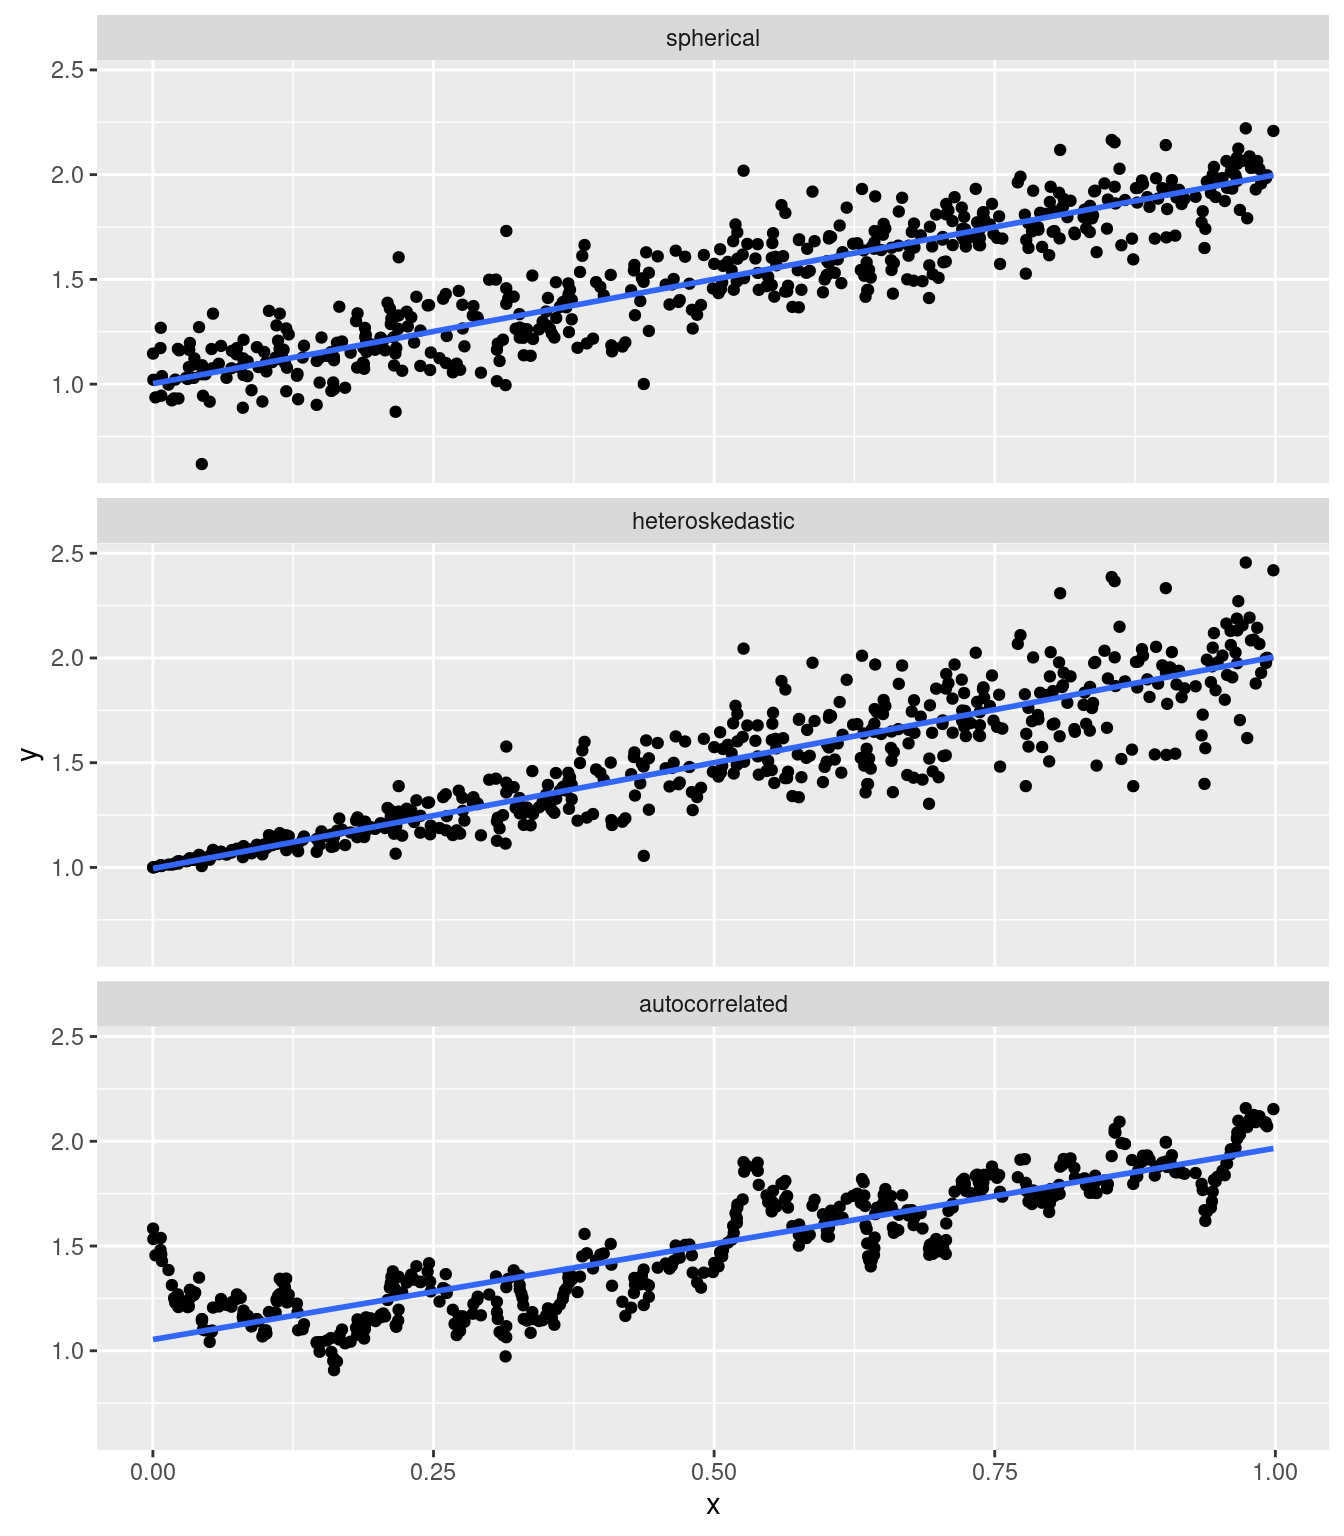
\includegraphics{pdaps_files/figure-latex/spherical-errors-1.pdf}

Notice that in the right-hand graph, the distribution of errors around the regression line is uneven---the spread is much greater at greater values of the covariate.

According to the Gauss-Markov theorem, if the errors are spherical, then OLS is the \emph{best linear unbiased estimator (BLUE)} of the linear model parameters \(\beta\). By ``best,'' we mean that it is efficient---any other linear unbiased estimator has larger standard errors. In other words, under the spherical error condition, any estimator \(\hat{\beta}\) with a smaller standard errors than OLS must either be:

\begin{itemize}
\item
  Biased: \(E[\hat{\beta}] \neq \beta\).
\item
  Nonlinear: \(\hat{\beta}\) cannot be written as a linear function of \(Y\).
\end{itemize}

Much later in the course, we will encounter ridge regression, a linear estimator that has lower standard errors than OLS. The Gauss-Markov theorem tells us that we're making a tradeoff when we use ridge regression---that we're taking on some bias in exchange for the reduction in variance.

\hypertarget{specification}{%
\chapter{Specification Issues}\label{specification}}

\providecommand{\pderiv}{}
\renewcommand{\pderiv}[2]{\frac{\partial{}#1}{\partial{}#2}}

I lied to you about the linear model last week. Like the grade-school teachers who told you everyone thought the world was flat before Columbus proved them wrong, I had good intentions---but it was a lie nonetheless.

I claimed that the linear model assumed that the conditional expectation of the response was a linear function of the covariates. That is false. A data model is a linear model, can be estimated consistently and without bias by OLS, and all that good stuff, as long as it is linear in the \emph{parameters}.

For example, the following is a linear model.
\[
Y_n = \beta_1 + \beta_2 x_n + \beta_3 x_n^2 + \beta_4 x_n^7 + \epsilon_n.
\]
The conditional expectation of \(Y_n\) is a nonlinear function of \(x_n\) (holding \(\beta\) fixed) but a linear function of \(\beta\) (holding \(x_n\) fixed). Therefore, assuming strict exogeneity holds, OLS is an unbiased, consistent, asymptotically normal estimator of \(\beta\).

The following is not a linear model.
\[
Y_n = 2^{\beta_1} + 2^{\beta_2} x_n + \epsilon_n.
\]
Holding \(\beta\) fixed, this is a linear function of the covariate \(x_n\). But, holding \(x_n\) fixed, this is not a linear function of \(\beta\). OLS is not an appropriate estimator for the parameters of this model.

This week, we will talk about linear models with non-standard covariate specifications---those that aren't just a linear function of continuous variables.

\hypertarget{categorical-variables}{%
\section{Categorical Variables}\label{categorical-variables}}

Using the linear model, we write the conditional expectation for the \(n\)'th response as
\[
E[Y_n \,|\, \mathbf{x}_n] = \mathbf{x}_n \cdot \beta + \epsilon_n,
\]
where \(\mathbf{x}_n\) is the vector of \(K\) covariates (including the intercept) and \(\beta\) is the vector of \(K\) coefficients we wish to estimate.

This makes sense with numerical variables, but not so much with categorical variables. For example, think of the relationship between party identification and one's vote in the 2016 presidential election. Suppose our response variable is one's vote (1 for Trump, 0 for non-Trump), and our party ID variable records whether the respondent is a Republican, Democrat, or independent. The resulting linear model equation,
\[
\text{Trump}_n = \beta_1 + \beta_2 \text{Party ID}_n + \epsilon_n,
\]
doesn't really make sense, because party ID isn't a number.\footnote{Oldish-school political scientists, by which I mean just about anyone who got their PhD between 1990 and 2010, would now be clutching their pearls at the mere thought of using a linear model for vote choice. But so-called ``binary dependent variable'' models like logistic regression are at best overrated, as you read in \emph{Mostly Harmless Econometrics}.}

To incorporate a categorical variable into the linear model, we break each category into its own binary variable. For example, with our party ID variable, we go from
\[
\text{Party ID} = \begin{pmatrix}
\text{R} \\
\text{R} \\
\text{I} \\
\text{I} \\
\text{D} \\
\text{D}
\end{pmatrix}
\]
to
\[
\text{Republican} = \begin{pmatrix} 1 \\ 1 \\ 0 \\ 0 \\ 0 \\ 0 \end{pmatrix},
\text{Independent} = \begin{pmatrix} 0 \\ 0 \\ 1 \\ 1 \\ 0 \\ 0 \end{pmatrix},
\text{Democratic} = \begin{pmatrix} 0 \\ 0 \\ 0 \\ 0 \\ 1 \\ 1 \end{pmatrix}.
\]
These are called \emph{dummy variables} or, preferably, \emph{indicator variables}.

Having turned our categorical variable into a set of indicators, you may be tempted to rewrite the model as
\[
\text{Trump}_n = \beta_1 + \beta_2 \text{Republican}_n + \beta_3 \text{Independent}_n + \beta_4 \text{Democratic}_n + \epsilon_n.
\]
But take a look at the matrix of covariates, or \emph{design matrix}, that would result if we set up the model this way:
\[
\mathbf{X} = \begin{bmatrix}
  1 & 1 & 0 & 0 \\
  1 & 1 & 0 & 0 \\
  1 & 0 & 1 & 0 \\
  1 & 0 & 1 & 0 \\
  1 & 0 & 0 & 1 \\
  1 & 0 & 0 & 1
\end{bmatrix}
\]
The columns of the design matrix are linearly dependent: the constant term is equal to the sum of three party ID indicators. (A useful exercise is to calculate \(\mathbf{X}^\top \mathbf{X}\) and confirm that its columns are linearly dependent too.) This means we can't include all three when estimating \(\beta\) via OLS---we have to drop one category.

In one sense, which category we drop is immaterial---our regression will make the same predictions either way. However, in order to interpret the results of a regression on categorical variables, it is important that we know what the categories are, and which one has been dropped.

For example, imagine we drop the Republican category, so we have the following linear model:
\[
\text{Trump}_n = \beta_1 + \beta_2 \text{Independent}_n + \beta_3 \text{Democratic}_n + \epsilon_n.
\]
For a Republican voter, the Independent and Democratic variables will both equal zero, so we will have
\[
E[\text{Trump}_n \,|\, \text{Party ID}_n = \text{R}] = \beta_1.
\]
In other words, the intercept will be the predicted probability that a Republican votes for Trump. For an Independent voter, we will have
\[
E[\text{Trump}_n \,|\, \text{Party ID}_n = \text{I}] = \beta_1 + \beta_2.
\]
So the coefficient on the Independent indicator is not the predicted probability that an Independent votes for Trump. Instead, it is the \emph{difference} in probability of a Trump vote between Independents and the baseline category (in this case, Republicans).

\begin{itemize}
\item
  If Independents are less likely than Republicans to vote for Trump, the coefficient on Independent will be negative.
\item
  If Independents are more likely than Republicans to vote for Trump, the coefficient on Independent will be positive.
\item
  If Independents are equally likely as Republicans to vote for Trump, the coefficient on Independent will be zero.
\end{itemize}

Similarly, for a Democratic voter, we have
\[
E[\text{Trump}_n \,|\, \text{Party ID}_n = \text{D}] = \beta_1 + \beta_3.
\]
The interpretation of the coefficient on Democratic is the same as for the coefficient on Independent.

Take a look at the following results of a hypothetical regression.

\begin{longtable}[]{@{}ll@{}}
\toprule
Coefficient & Estimate\tabularnewline
\midrule
\endhead
(Intercept) & 0.9\tabularnewline
Independent & -0.4\tabularnewline
Democratic & -0.75\tabularnewline
\bottomrule
\end{longtable}

\begin{itemize}
\item
  Republicans have a 90\% chance of voting for Trump. We see that by looking at the intercept, since Republicans are the omitted category.
\item
  We see from the coefficient on Independent that an Independent's chance of voting for Trump is 40\% lower than a Republican's. This means that an Independent has a 50\% chance of voting for Trump.
\item
  Similarly, we see from the coefficient on Democratic that a Democrat's chance of voting for Trump is 75\% lower than a Republican's, for a 15\% chance overall.
\end{itemize}

Had we instead omitted Independent, we would get different coefficients, but the same predictions.

\begin{longtable}[]{@{}ll@{}}
\toprule
Coefficient & Estimate\tabularnewline
\midrule
\endhead
(Intercept) & 0.5\tabularnewline
Republican & 0.4\tabularnewline
Democratic & -0.35\tabularnewline
\bottomrule
\end{longtable}

Same story, different numbers, had we omitted Democratic.

\begin{longtable}[]{@{}ll@{}}
\toprule
Coefficient & Estimate\tabularnewline
\midrule
\endhead
(Intercept) & 0.15\tabularnewline
Republican & 0.75\tabularnewline
Independent & 0.35\tabularnewline
\bottomrule
\end{longtable}

Given that the results are substantively the same no matter what, does it matter which category we choose to drop? Yes, for the purpose of communicating your results. The omitted category should serve as a meaningful baseline. For this example, all of our three categories are substantively meaningful, so any choice will do. But imagine replacing our part ID variable with a race variable that has the following categories:

\begin{itemize}
\tightlist
\item
  White
\item
  Black
\item
  Hispanic
\item
  Asian
\item
  Other
\end{itemize}

You may be tempted to make ``Other'' the excluded category, so that you obtain a coefficient for each of the specific racial groups. But that's actually the worst choice possible. The coefficient on the White variable would then represent the difference in probability of voting for Trump between a white voter and a voter in the ``other'' category---which is hard to interpret. Whereas if we instead omitted the Black category, the coefficient on the White variable would represent the difference between white and black voters.

When in doubt, I recommend omitting whichever category is largest in the data.

Now let's introduce covariates into the mix. Consider a regression of Trump vote on party ID (Republican as omitted category) and age, producing the following results.

\begin{longtable}[]{@{}ll@{}}
\toprule
Coefficient & Estimate\tabularnewline
\midrule
\endhead
(Intercept) & 0.8\tabularnewline
Independent & -0.4\tabularnewline
Democratic & -0.75\tabularnewline
Age & 0.002\tabularnewline
\bottomrule
\end{longtable}

Remember what the coefficient of 0.002 on Age means: if we compared one voter to another who was otherwise identical (in this case, same Party ID) except five years older, we would expect the latter voter to have a 1\% greater chance of voting for Trump.

More specifically, we have three different regression lines---one for each group:
\[
\begin{aligned}
  E[\text{Trump}_n \,|\, \text{Party ID}_n = \text{R}, \text{Age}_n] &= 0.8 + 0.002 \text{Age}_n, \\
  E[\text{Trump}_n \,|\, \text{Party ID}_n = \text{I}, \text{Age}_n] &= 0.4 + 0.002 \text{Age}_n, \\
  E[\text{Trump}_n \,|\, \text{Party ID}_n = \text{D}, \text{Age}_n] &= 0.05 + 0.002 \text{Age}_n.
\end{aligned}
\]
Notice that the slope is the same in each regression line. Only the intercept varies across groups. When we include a categorical variable in a regression model, it's like allowing the intercept to differ across categories.

\hypertarget{interaction-terms}{%
\section{Interaction Terms}\label{interaction-terms}}

When political scientists or economists describe their regression results, they will often talk about the marginal effects of different variables. Formally, the \emph{marginal effect} of the \(k\)'th covariate, \(x_{nk}\), is
\[
\frac{\partial{}E[Y_n \,|\, \mathbf{x}_n]}{\partial{}x_{nk}},
\]
the partial derivative of the conditional expectation with respect to the \(k\)'th covariate.

The marginal effect answers the following question: Suppose we have two observations that differ in the \(k\)'th covariate by one unit, but are otherwise identical. How much greater, or less, would we expect the response to be for the observation with the one-unit-greater value of \(x_{nk}\)?

If we were sure the relationship we were modeling were causal, we could phrase the above question more succinctly. We could ask: Given a one-unit change in the \(k\)'th covariate, holding all else fixed, what change in the response should we expect? But we haven't yet gotten to the point where we can make our claims causal. Hence I will often refer to \emph{so-called marginal effects}, since I don't want the ``effect'' terminology to deceive us into thinking we're drawing causal inferences. So-called marginal effects are just a nice way to summarize the relationship between individual covariates and the conditional expectation.

The bare-bones linear model has the (sometimes appealing, sometimes not) feature that it assumes constant marginal effects. For each covariate \(x_{nk}\), we have
\[
\frac{\partial{}E[Y_n \,|\, \mathbf{x}_n]}{\partial{}x_{nk}} = \beta_k,
\]
the coefficient on that covariate. This encodes two critical assumptions:

\begin{enumerate}
\def\labelenumi{\arabic{enumi}.}
\item
  The marginal effect of the \(k\)'th covariate does not depend on the value of any other covariates.
\item
  The marginal effect of the \(k\)'th covariate does not depend on its own value.
\end{enumerate}

It is easy to think of scenarios where each of these might be questionable.

\begin{enumerate}
\def\labelenumi{\arabic{enumi}.}
\item
  Imagine a study of individual voters' choices in U.S. House races, where we model voting for the incumbent as a function of how often the voter goes to church. The marginal effect of religiosity is probably different if the incumbent is a Republican than if the incumbent is a Democrat.
\item
  Imagine a study of individual voters' turnout decisions, where we model turnout as a function of the voter's ideology. Suppose ideology is measured on a 7-point scale, where 1 is most liberal and 7 is most conservative. We know the most ideologically extreme voters are the most likely to turn out. So, all else equal, we'd expect moving from 1 to 2 (very liberal to pretty liberal) to decrease one's probability of voting, but we'd expect moving from 6 to 7 (pretty conservative to very conservative) to increase one's probability of voting.
\end{enumerate}

Let's start with the first case, where the (so-called) marginal effect of one variable depends on the value of another variable. To allow for this in our models, we include the product of the two covariates in our model.

For example, suppose we are interested in whether the relationship between education and voting for Trump is different between whites and non-whites. We would include three terms in the model (plus an intercept): education, an indicator for white, and their product.
\[
\text{Trump}_n = \beta_1 + \beta_2 \text{Education}_n + \beta_3 \text{White}_n + \beta_4 (\text{Education}_n \times \text{White}_n) + \epsilon_n.
\]
The so-called marginal effect of education is now
\[
\frac{\partial{}E[\text{Trump}_n \,|\, \mathbf{x}_n]}{\partial{}\text{Education}_n}
= \beta_2 + \beta_4 \text{White}_n.
\]
This equation tells us three things.

\begin{itemize}
\item
  \(\beta_2\) is the marginal effect of education for non-white voters.
\item
  \(\beta_4\) is the difference between the marginal effect of education for white voters and the effect for non-white voters.
\item
  \(\beta_2 + \beta_4\) is the marginal effect of education for white voters.
\end{itemize}

Another way to think of it is that we have two regression lines:
\[
\begin{aligned}
  E[\text{Trump}_n \,|\, \text{White}_n = 0, \text{Education}_n] &= \beta_1 + \beta_2 \text{Education}_n, \\
  E[\text{Trump}_n \,|\, \text{White}_n = 1, \text{Education}_n] &= (\beta_1 + \beta_3) + (\beta_2 + \beta_4) \text{Education}_n.
\end{aligned}
\]
We saw before that including a categorical variable is like allowing a different intercept for each category. Including an interaction with a categorical variable is like allowing a different slope for each category.

At this point, you might ask, why not just run two separate regressions? I can think of at least two reasons not to.

\begin{itemize}
\item
  You might want to include other covariates whose effects you don't think are dependent on race (e.g., age). If you ran separate regressions, you would estimate race-dependent effects for every covariate, at a potential loss of efficiency.
\item
  You might want to formally test the hypothesis that the effect of education is equal for whites and non-whites. This is easiest to do if you have a single model. Next week we will talk about the tools you would need to undertake this sort of test.
\end{itemize}

One frequent source of confusion with interaction terms is whether you need to include lower-order terms in the model. For example, if we are only interested in how the effect of education differs with race, why can't we just include education and its product with race in the specification? The equations above give you the answer. Leaving the white indicator out of the model is like fixing \(\beta_3 = 0\). This means you're forcing the regression lines for whites and non-whites to have the same intercept, which there's no good reason to do.

If you're not yet persuaded on the necessity of including constitutive terms of interactions in your regressions, see \citet{braumoeller2004hypothesis}.

For an example of interaction terms, imagine the following example. Suppose education is measured in years of schooling.

\begin{longtable}[]{@{}ll@{}}
\toprule
Coefficient & Estimate\tabularnewline
\midrule
\endhead
(Intercept) & 0.3\tabularnewline
Education & 0.01\tabularnewline
White & 0.4\tabularnewline
Education * White & -0.03\tabularnewline
\bottomrule
\end{longtable}

We would interpret these in the following way.

\begin{itemize}
\item
  A hypothetical non-white voter with zero years of education has a 30\% chance of voting for Trump. For each additional year of education, the probability of voting for Trump goes up by 1\%.
\item
  A hypothetical white voter with zero years of education has a 70\% (0.3 + 0.4) chance of voting for Trump. For each additional year of education, the probability of voting for Trump goes down by 2\% (0.01 - 0.03).
\end{itemize}

What about an interaction between two continuous variables? For example, imagine an interaction between age and education in our model of voting for Trump.

\begin{longtable}[]{@{}ll@{}}
\toprule
Coefficient & Estimate\tabularnewline
\midrule
\endhead
(Intercept) & 0.4\tabularnewline
Education & -0.02\tabularnewline
Age & 0.002\tabularnewline
Education * Age & 0.0002\tabularnewline
\bottomrule
\end{longtable}

One simple way to interpret the effect of each variable is to hold the other one fixed at various values. For example, for a 20-year-old, we have
\[
\begin{aligned}
E[\text{Trump}_n \,|\, \text{Age}_n = 20, \text{Education}_n] &= 0.44 - 0.16 \text{Education}_n,
\end{aligned}
\]
whereas for an 80-year-old, we have
\[
\begin{aligned}
E[\text{Trump}_n \,|\, \text{Age}_n = 80, \text{Education}_n] &= 0.56 - 0.04 \text{Education}_n.
\end{aligned}
\]
These results would seem to imply that (1) older people have a higher baseline probability of voting for Trump, and (2) the magnitude of the negative relationship between education and voting for Trump is weaker for older voters.

Always remember: when in doubt, take the partial derivative of \(Y_n\) (or, more precisely, its conditional expectation) with respect to the variable you're interested in. For example, here we have
\[
\frac{\partial{}E[\text{Trump}_n \,|\, \mathbf{x}_n]}{\partial{}\text{Education}_n} = -0.02 + 0.0002 \text{Age}_n.
\]

\hypertarget{quadratic-terms}{%
\section{Quadratic Terms}\label{quadratic-terms}}

We use interaction terms when the marginal effect of one variable depends on the value of another variable. But sometimes the marginal effect of a variable depends on its \emph{own} value. The most stark example is a ``U-shaped'' relationship, such as we expect between ideology and voter turnout.

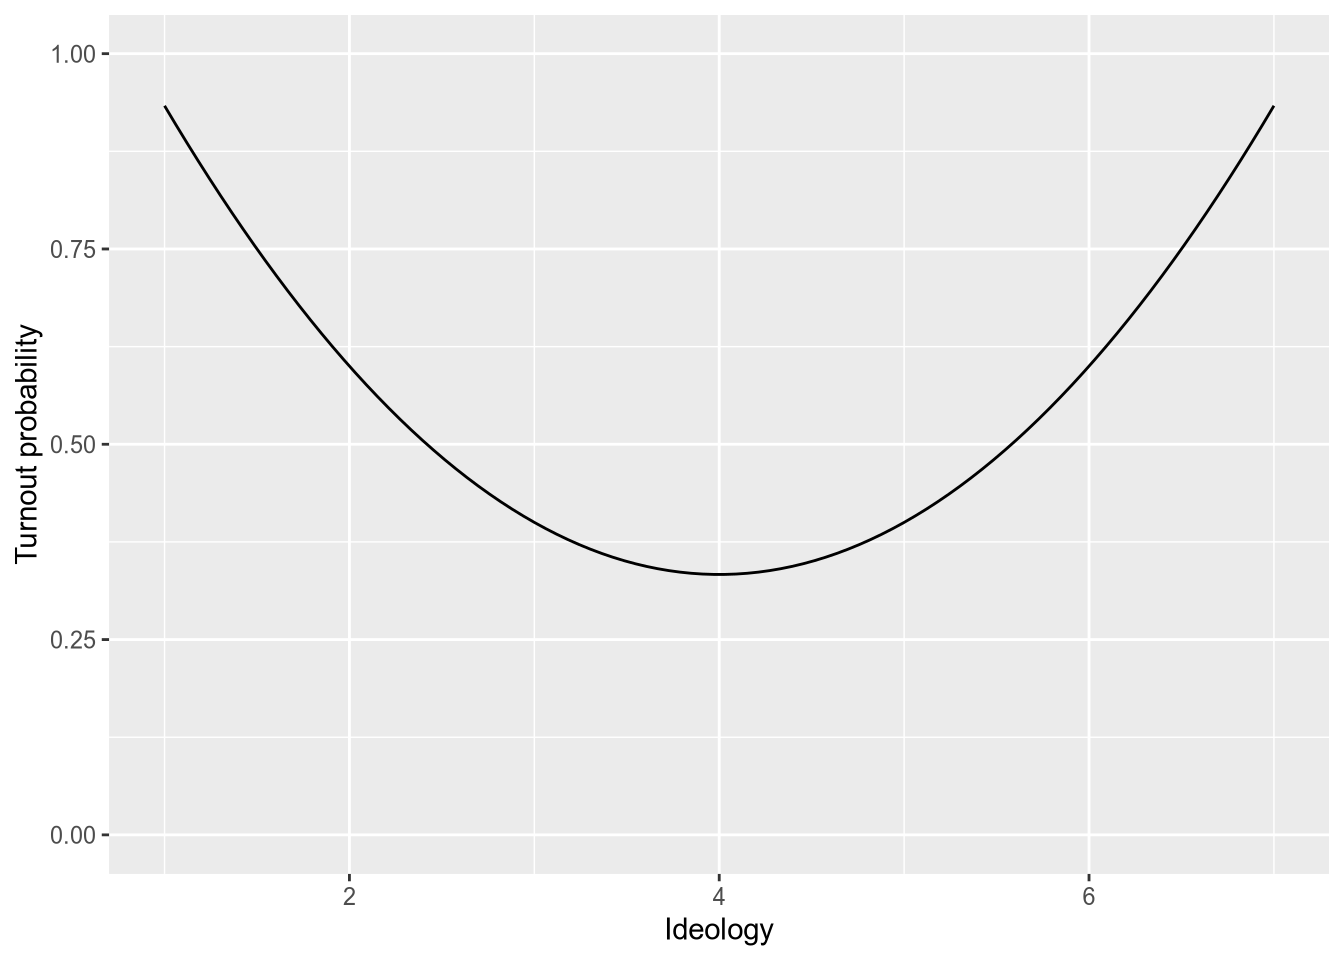
\includegraphics{pdaps_files/figure-latex/u-shaped-1.pdf}

We call this kind of relationship \emph{non-monotonic}, since it is neither increasing everywhere nor decreasing everywhere. However, even with a monotonic relationship, the marginal effect might depend on the value of the variable. (In other words, while every linear function is monotonic, not every monotonic function is linear.) For example, think of a hockey-stick shaped relationship.

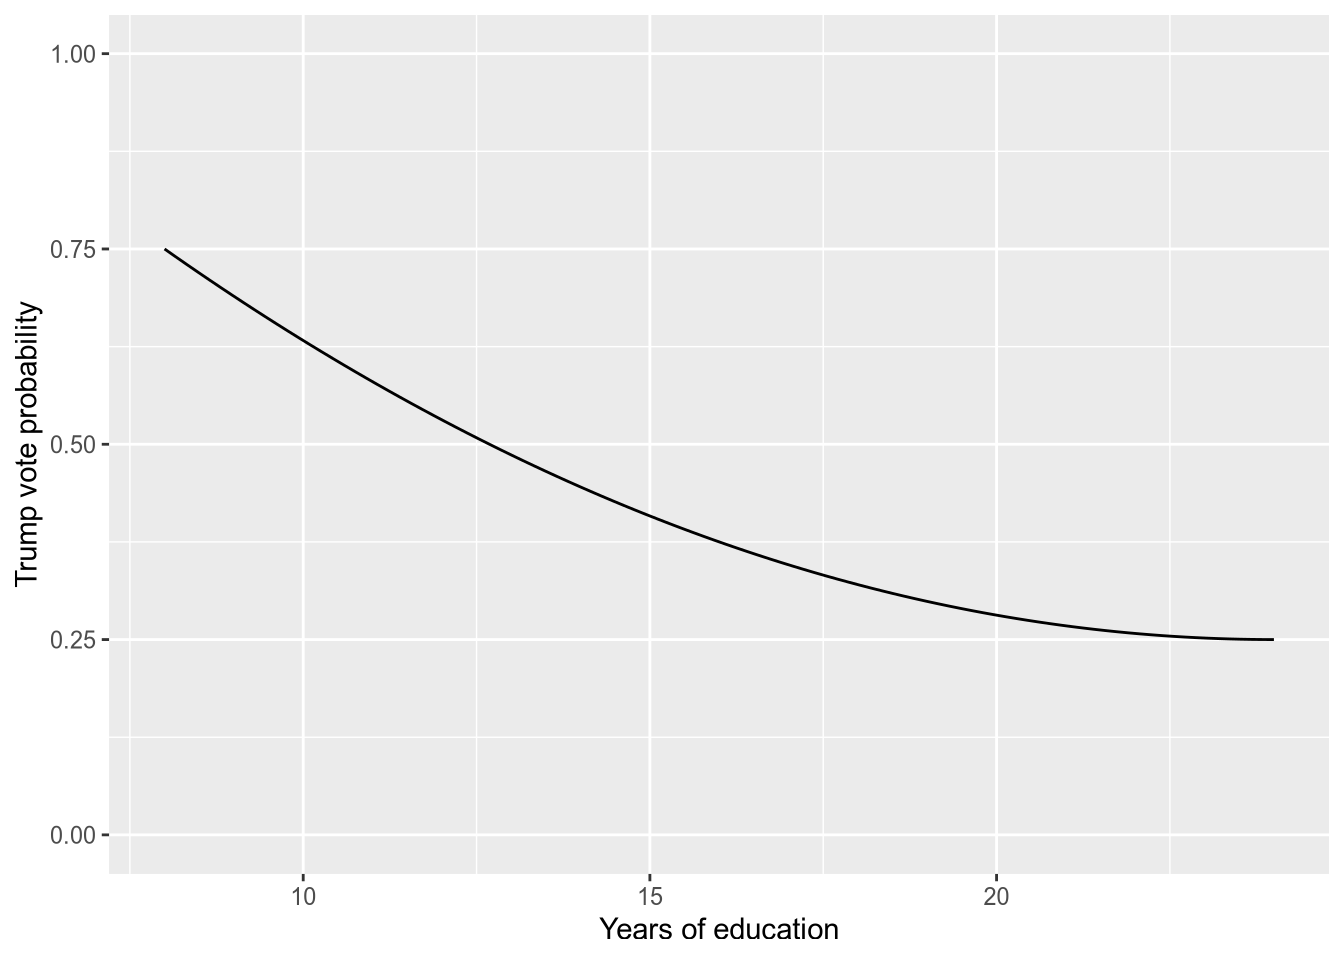
\includegraphics{pdaps_files/figure-latex/hockey-stick-1.pdf}

If we model the relationship between years of education and voting for Trump as linear, then we impose the assumption that the difference between voters with 16 years of education and 12 years of education (college versus high-school graduates) is the same as between those with 24 and 20 years of education (got the PhD slowly versus got the PhD quickly). Depending on our sample and the goal of our study, that may not be a reasonable assumption (or approximation).

We typically use quadratic models for non-monotonic relationships. In the example above, this would entail a regression model like
\[
\text{Turnout}_n = \beta_1 + \beta_2 \text{Ideology}_n + \beta_3 \text{Ideology}_n^2 + \epsilon_n.
\]
Under this model, the marginal effect of Ideology is
\[
\frac{\partial{}E[\text{Turnout}_n \,|\, \text{Ideology}_n]}{\partial{}\text{Ideology}_n}
= \beta_2 + 2 \beta_3 \text{Ideology}_n.
\]

\begin{itemize}
\item
  If \(\beta_3\) is positive, that means the effect of Ideology increases with the value of Ideology, representing a U-shaped relationship.
\item
  If \(\beta_3\) is negative, that means the effect of Ideology decreases with the value of Ideology, representing an inverse-U-shaped relationship.
\item
  If \(\beta_3\) is zero, that means the effect of Ideology is constant.
\end{itemize}

\hypertarget{logarithmic-models}{%
\section{Logarithmic Models}\label{logarithmic-models}}

The last common form of nonlinear specification is when we take the natural logarithm of a covariate, the response, or both.

To set a baseline, let's remember the standard bivariate linear model,
\[
Y_n = \beta_1 + \beta_2 x_n + \epsilon_n.
\]
Under the standard model, we say that a 1-unit difference in \(x_n\) is associated with a \(\beta_2\)-unit difference in \(Y_n\).
In other words, the so-called marginal effect of \(x_n\) is the constant \(\beta_2\).

Now consider a specification in which we instead model \(Y_n\) as a function of the natural logarithm of \(x_n\):
\[
Y_n = \beta_1 + \beta_2 \log x_n + \epsilon_n.
\]
As always, we can calculate the so-called marginal effect by taking the partial derivative:
\[
\frac{\partial{}E[Y_n \,|\, x_n]}{\partial{}x_n} = \frac{\beta_2}{x_n}.
\]
This tells us that as \(x_n\) grows larger, the magnitude of the so-called marginal effect diminishes, as in the following illustrations.

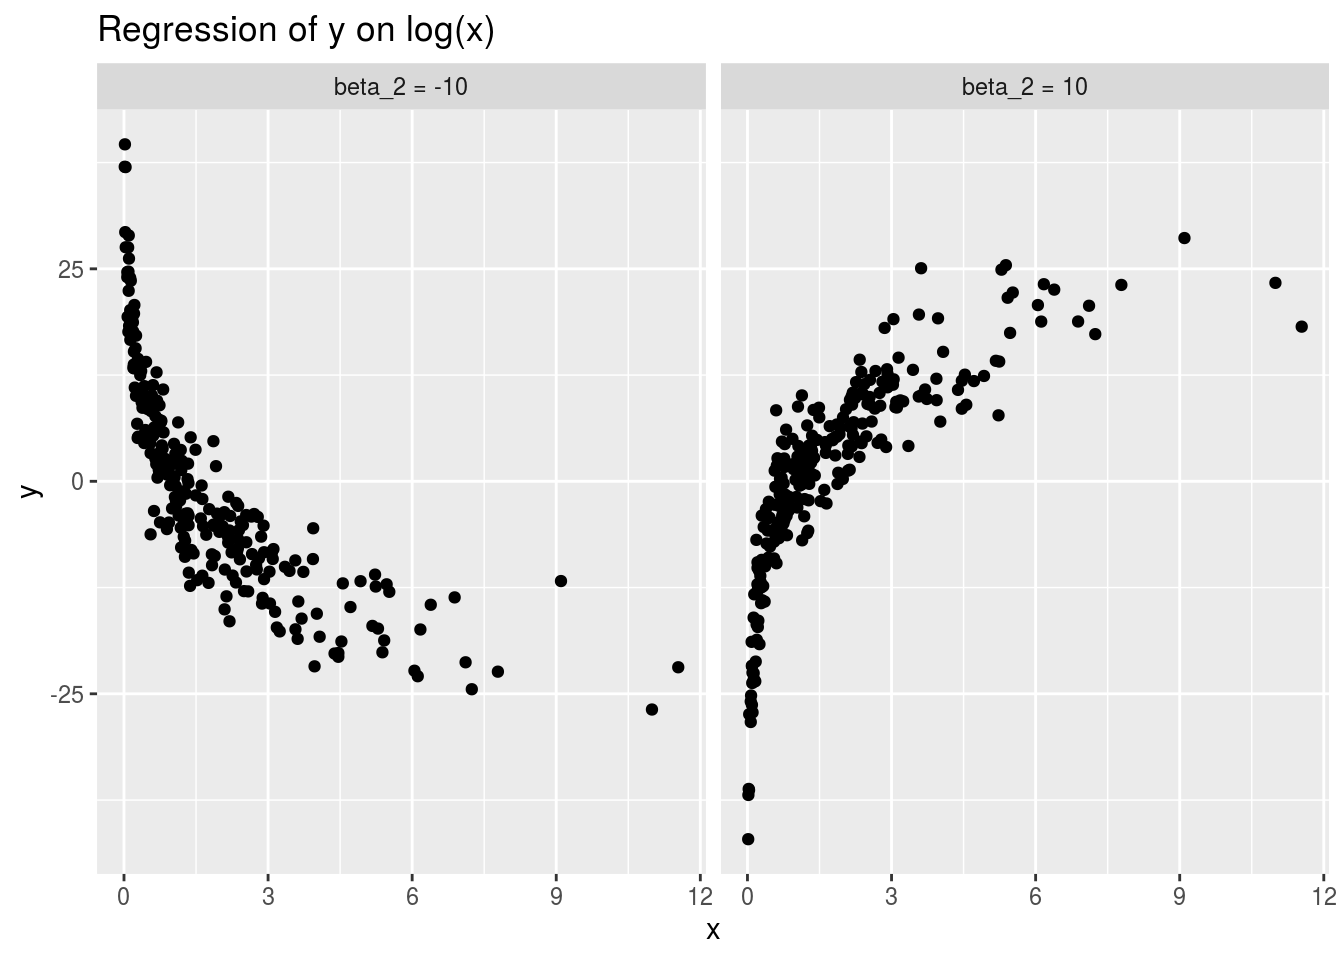
\includegraphics{pdaps_files/figure-latex/lin-log-1.pdf}

One way to interpret this kind of specification is that a 1 \emph{percent} increase in \(x_n\) is associated with a \(\frac{\beta_2}{100}\) \emph{unit} change in \(Y_n\).
To see why, we will rely on two fun facts: that \(\log(a \times b) = \log a + \log b\) and that \(\log(1 + x) \approx x\) for small \(x\) (roughly \(|x| < 0.1\)).
Now let \(Y_n\) be the baseline value of the response, and let \(Y_n'\) be the counterfactual value under a 1 percent increase in \(x_n\).
Then we have
\[
\begin{aligned}
Y_n' - Y_n
&= \beta_2 (\log(1.01 x_n) - \log x_n) \\
&= \beta_2 (\log 1.01 + \log x_n - \log x_n) \\
&= \beta_2 \log 1.01 \\
&\approx 0.01 \beta_2.
\end{aligned}
\]

Conversely, you may see a specification in which the response is logged and the covariate is not:
\[
\log Y_n = \beta_1 + \beta_2 x_n + \epsilon_n.
\]
For positive \(\beta_2\), this means the so-called marginal effect of \(x_n\) \emph{increases} as \(x_n\) grows large.
Similarly, for negative \(\beta_2\), this means the so-called marginal effect of \(x_n\) increases as \(x_n\) decreases.

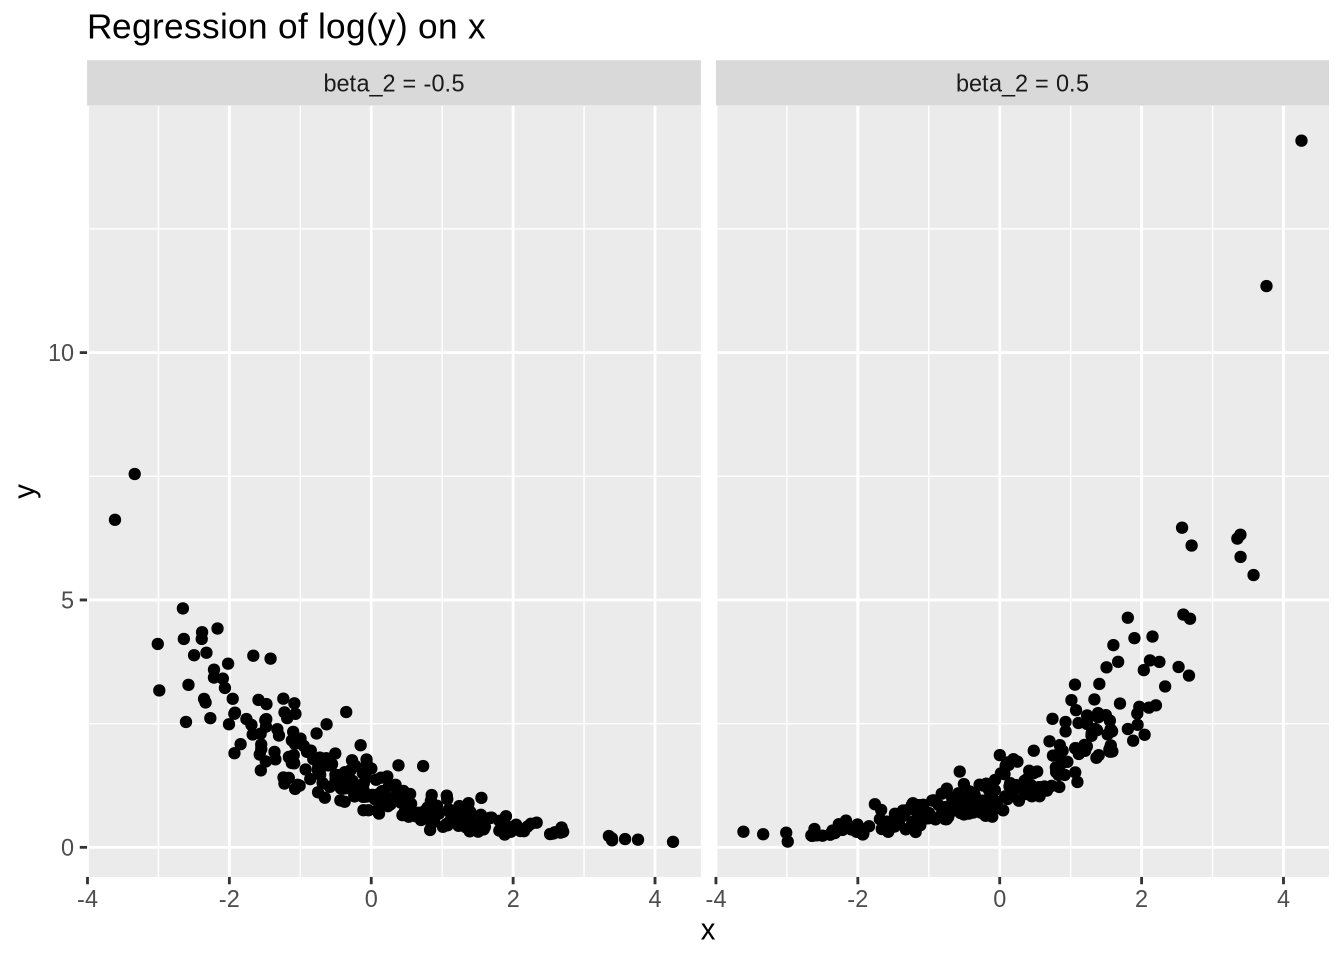
\includegraphics{pdaps_files/figure-latex/log-lin-1.pdf}

To interpret this specification, we say that a 1 \emph{unit} increase in \(x_n\) is associated with a \(100(e^{\beta_2} - 1)\) \emph{percent} change in \(Y_n\).
For example, with a coefficient of \(\beta_2 = 0.5\), we would say a 1 unit increase in \(x_n\) is associated with a 65\% increase in \(Y_n\), as \(e^{0.5} \approx 1.65\).
To see why this is the case, let \(Y_n\) be the baseline value of the response, and let \(Y_n'\) be the counterfactual value under a 1 unit increase in \(x_n\).
Then, as observed by \citet[93--94]{angrist2015mastering}, we have
\[
\log \frac{Y_n'}{Y_n} = \log Y_n' - \log Y_n = \beta_2,
\]
and therefore
\[
Y_n' = \exp(\beta_2) Y_n.
\]
Conveniently, for small values of \(\beta_2\) (roughly \(|\beta_2| < 0.1\)), we have \(\exp(\beta_2) - 1 \approx \beta_2\).
For example, if \(\beta_2 = -0.05\), then we would say that a 1 unit increase in \(x_n\) is associated with a 5\% decrease in \(Y_n\).

Last, consider the model in which the covariate and the response are both logged:
\[
\log Y_n = \beta_1 + \beta_2 \log X_n + \epsilon_n.
\]

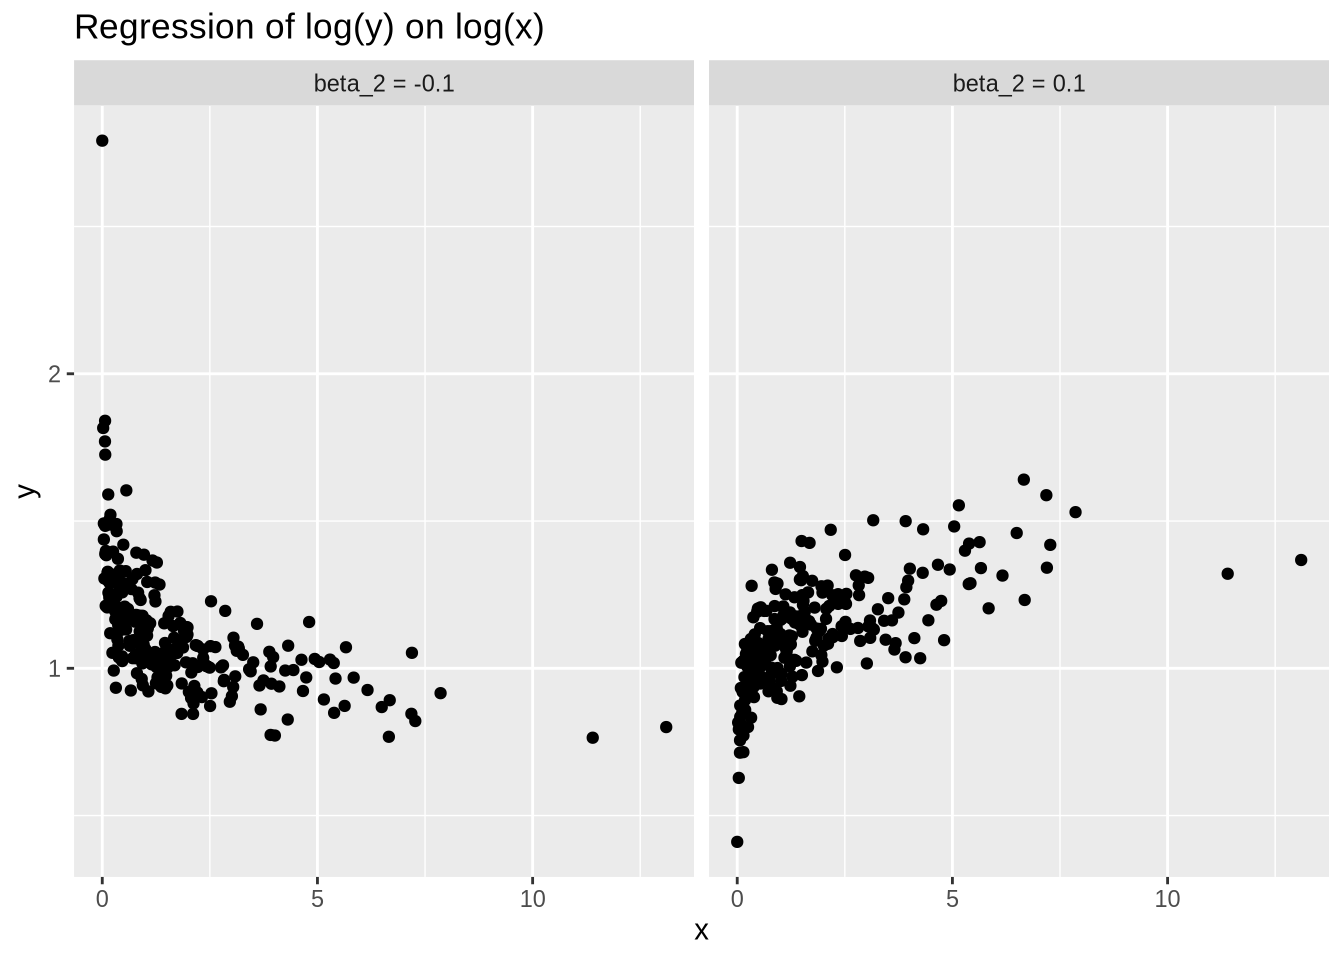
\includegraphics{pdaps_files/figure-latex/log-log-1.pdf}

In the last two specifications, we interpreted the term that was logged in terms of percentage changes.
The same is true here: the log-log model relates percent changes in \(x_n\) to percent changes in \(Y_n\).
Specifically, we say that a 1 percent increase in \(x_n\) is associated with a \(\beta_2\) percent change in \(Y_n\).
To see why, again let \(Y_n\) be a baseline value, and let \(Y_n'\) be the counterfactual if we increased \(x_n\) by 1 percent.
Then we have
\[
\begin{aligned}
\log \frac{Y_n'}{Y_n}
&= \beta_2 (\log(1.01 x_n) - \log x_n) \\
&= (\log 1.01) \beta_2 \\
&\approx 0.01 \beta_2,
\end{aligned}
\]
which in turn gives us
\[
Y_n' \approx \exp(0.01 \beta_2) Y_n \approx (1 + 0.01 \beta_2) Y_n.
\]
For example, in the log-log model, a coefficient of \(\beta_2 = 0.5\) means that a 1 percent increase in \(x_n\) is associated with a 0.5 percent increase in \(Y_n\).

To summarize, here are the four possible logarithmic specifications and their interpretations:

\begin{longtable}[]{@{}lll@{}}
\toprule
\begin{minipage}[b]{0.24\columnwidth}\raggedright
Response\strut
\end{minipage} & \begin{minipage}[b]{0.26\columnwidth}\raggedright
Covariate\strut
\end{minipage} & \begin{minipage}[b]{0.41\columnwidth}\raggedright
Interpretation\strut
\end{minipage}\tabularnewline
\midrule
\endhead
\begin{minipage}[t]{0.24\columnwidth}\raggedright
\(Y_n\)\strut
\end{minipage} & \begin{minipage}[t]{0.26\columnwidth}\raggedright
\(x_n\)\strut
\end{minipage} & \begin{minipage}[t]{0.41\columnwidth}\raggedright
1 unit increase in \(x_n\) \(\Rightarrow\) \(\beta\) unit change in \(Y_n\)\strut
\end{minipage}\tabularnewline
\begin{minipage}[t]{0.24\columnwidth}\raggedright
\(Y_n\)\strut
\end{minipage} & \begin{minipage}[t]{0.26\columnwidth}\raggedright
\(\log x_n\)\strut
\end{minipage} & \begin{minipage}[t]{0.41\columnwidth}\raggedright
1 percent increase in \(x_n\) \(\Rightarrow\) \(\beta / 100\) unit change in \(Y_n\)\strut
\end{minipage}\tabularnewline
\begin{minipage}[t]{0.24\columnwidth}\raggedright
\(\log Y_n\)\strut
\end{minipage} & \begin{minipage}[t]{0.26\columnwidth}\raggedright
\(x_n\)\strut
\end{minipage} & \begin{minipage}[t]{0.41\columnwidth}\raggedright
1 unit increase in \(x_n\) \(\Rightarrow\) \(100(e^\beta - 1)\) percent change in \(Y_n\)\strut
\end{minipage}\tabularnewline
\begin{minipage}[t]{0.24\columnwidth}\raggedright
\(\log Y_n\)\strut
\end{minipage} & \begin{minipage}[t]{0.26\columnwidth}\raggedright
\(\log x_n\)\strut
\end{minipage} & \begin{minipage}[t]{0.41\columnwidth}\raggedright
1 percent increase in \(x_n\) \(\Rightarrow\) \(\beta\) percent change in \(Y_n\)\strut
\end{minipage}\tabularnewline
\bottomrule
\end{longtable}

How do you decide which logarithmic model, if any, to use?

\begin{itemize}
\item
  You may let theory be your guide---develop expectations, on the basis of your substantive knowledge, about whether the relevant changes in conditional expectation will be in terms of levels or proportions.
\item
  Or you may be inductive---make scatterplots of all four possibilities, and choose the specification under which the relationship is closest to linear.
\end{itemize}

A final note on logarithmic models. The logarithm of a number \(c \leq 0\) does not exist. Therefore, a logarithmic model is only appropriate for a strictly positive response/covariate. For non-negative variables that include zeroes, some people try to ``fix'' this by doing \(\log(Y_n + 1)\), but in this situation it is generally better to follow the procedure advocated by \citet{burbidge1988alternative}.

\hypertarget{appendix-nonstandard-specifications-in-r}{%
\section{Appendix: Nonstandard Specifications in R}\label{appendix-nonstandard-specifications-in-r}}

We will use the following packages:

\begin{Shaded}
\begin{Highlighting}[]
\KeywordTok{library}\NormalTok{(}\StringTok{"tidyverse"}\NormalTok{)}
\KeywordTok{library}\NormalTok{(}\StringTok{"broom"}\NormalTok{)}
\KeywordTok{library}\NormalTok{(}\StringTok{"forcats"}\NormalTok{)}
\KeywordTok{library}\NormalTok{(}\StringTok{"interplot"}\NormalTok{)}
\end{Highlighting}
\end{Shaded}

\textbf{forcats} contains convenience functions for \emph{factors}, which are R's way of representing categorical variables. \textbf{interplot} is for plotting marginal effects from interactive models.

Once again, we will work with the occupational prestige data from the \textbf{car} package. We will also convert it to a tibble, so that it will more closely resemble the kind of data frame we would get had we read it in with \texttt{read\_csv()}.

\begin{Shaded}
\begin{Highlighting}[]
\KeywordTok{library}\NormalTok{(}\StringTok{"car"}\NormalTok{)}
\KeywordTok{data}\NormalTok{(Prestige)}
\NormalTok{Prestige \textless{}{-}}\StringTok{ }\KeywordTok{as\_tibble}\NormalTok{(Prestige)}

\NormalTok{Prestige}
\end{Highlighting}
\end{Shaded}

\begin{verbatim}
## # A tibble: 102 x 6
##   education income women prestige census type 
##       <dbl>  <int> <dbl>    <dbl>  <int> <fct>
## 1      13.1  12351 11.2      68.8   1113 prof 
## 2      12.3  25879  4.02     69.1   1130 prof 
## 3      12.8   9271 15.7      63.4   1171 prof 
## 4      11.4   8865  9.11     56.8   1175 prof 
## 5      14.6   8403 11.7      73.5   2111 prof 
## # ... with 97 more rows
\end{verbatim}

\hypertarget{categorical-variables-1}{%
\subsection{Categorical Variables}\label{categorical-variables-1}}

You will notice that the \texttt{type} column of the prestige data is listed as a \texttt{\textless{}fctr\textgreater{}}, which stands for factor. A factor is R's representation of a categorical variable. Let's take a closer look.

\begin{Shaded}
\begin{Highlighting}[]
\NormalTok{Prestige}\OperatorTok{$}\NormalTok{type}
\end{Highlighting}
\end{Shaded}

\begin{verbatim}
##   [1] prof prof prof prof prof prof prof prof prof prof prof prof prof prof prof
##  [16] prof prof prof prof prof prof prof prof prof prof prof prof bc   prof prof
##  [31] wc   prof wc   <NA> wc   wc   wc   wc   wc   wc   wc   wc   wc   wc   wc  
##  [46] wc   wc   wc   wc   wc   wc   wc   <NA> bc   wc   wc   wc   bc   bc   bc  
##  [61] bc   bc   <NA> bc   bc   bc   <NA> bc   bc   bc   bc   bc   bc   bc   bc  
##  [76] bc   bc   bc   bc   bc   bc   bc   bc   bc   bc   bc   bc   bc   bc   bc  
##  [91] bc   bc   bc   bc   bc   prof bc   bc   bc   bc   bc   bc  
## Levels: bc prof wc
\end{verbatim}

This looks kind of like---but isn't quite---a character variable. The most noticeable difference is that R tells us its \emph{levels}: the set of categories available. We can extract these directly with the \texttt{levels()} function.

\begin{Shaded}
\begin{Highlighting}[]
\KeywordTok{levels}\NormalTok{(Prestige}\OperatorTok{$}\NormalTok{type)}
\end{Highlighting}
\end{Shaded}

\begin{verbatim}
## [1] "bc"   "prof" "wc"
\end{verbatim}

This brings us to an important difference between \texttt{read.csv()} (with a dot, the built-in R function) and \texttt{read\_csv()} (with an underscore, the tidyverse version). The old way, \texttt{read.csv()}, by default treats any column of character strings as a factor. The tidyverse way, \texttt{read\_csv()}, never creates factors by default---you must make them explicitly.

To create a factor variable, you can use the \texttt{factor()} function:

\begin{Shaded}
\begin{Highlighting}[]
\NormalTok{example\_vector \textless{}{-}}\StringTok{ }\KeywordTok{c}\NormalTok{(}\DecValTok{4}\NormalTok{, }\DecValTok{1}\NormalTok{, }\DecValTok{3}\NormalTok{, }\DecValTok{3}\NormalTok{, }\DecValTok{1}\NormalTok{)}

\KeywordTok{factor}\NormalTok{(example\_vector,  }\CommentTok{\# vector to convert to factor}
       \DataTypeTok{levels =} \DecValTok{1}\OperatorTok{:}\DecValTok{4}\NormalTok{,    }\CommentTok{\# possible values of the vector}
       \DataTypeTok{labels =} \KeywordTok{c}\NormalTok{(}\StringTok{"ONE"}\NormalTok{,}
                  \StringTok{"two"}\NormalTok{,}
                  \StringTok{"Three"}\NormalTok{,}
                  \StringTok{"FOUR!"}\NormalTok{))  }\CommentTok{\# label corresponding to each value}
\end{Highlighting}
\end{Shaded}

\begin{verbatim}
## [1] FOUR! ONE   Three Three ONE  
## Levels: ONE two Three FOUR!
\end{verbatim}

Returning to the prestige data, let's run a regression of occupational prestige on occupational category.

\begin{Shaded}
\begin{Highlighting}[]
\NormalTok{fit\_type \textless{}{-}}\StringTok{ }\KeywordTok{lm}\NormalTok{(prestige }\OperatorTok{\textasciitilde{}}\StringTok{ }\NormalTok{type, }\DataTypeTok{data =}\NormalTok{ Prestige)}
\NormalTok{fit\_type}
\end{Highlighting}
\end{Shaded}

\begin{verbatim}
## 
## Call:
## lm(formula = prestige ~ type, data = Prestige)
## 
## Coefficients:
## (Intercept)     typeprof       typewc  
##      35.527       32.321        6.716
\end{verbatim}

\texttt{lm()} automatically converts the factor into a set of indicators, and automatically omits one category from the design matrix. In particular, it omits whichever level is listed first (which may not be the first level to appear in the data!). If you want to have a different category omitted, you need to reorder the levels, placing the category you want to omit first. You can do that with \texttt{fct\_relevel()} from the \textbf{forcats} package. Let's make white-collar (\texttt{wc}) the omitted category.

\begin{Shaded}
\begin{Highlighting}[]
\NormalTok{Prestige}\OperatorTok{$}\NormalTok{type \textless{}{-}}\StringTok{ }\KeywordTok{fct\_relevel}\NormalTok{(Prestige}\OperatorTok{$}\NormalTok{type, }\StringTok{"wc"}\NormalTok{)}
\KeywordTok{levels}\NormalTok{(Prestige}\OperatorTok{$}\NormalTok{type)}
\end{Highlighting}
\end{Shaded}

\begin{verbatim}
## [1] "wc"   "bc"   "prof"
\end{verbatim}

\begin{Shaded}
\begin{Highlighting}[]
\NormalTok{fit\_type\_relevel \textless{}{-}}\StringTok{ }\KeywordTok{lm}\NormalTok{(prestige }\OperatorTok{\textasciitilde{}}\StringTok{ }\NormalTok{type, }\DataTypeTok{data =}\NormalTok{ Prestige)}
\end{Highlighting}
\end{Shaded}

We can confirm by checking out the model fit statistics that which category we omit makes no difference to the overall fit of the model, or the predicted values.

\begin{Shaded}
\begin{Highlighting}[]
\KeywordTok{glance}\NormalTok{(fit\_type)}
\end{Highlighting}
\end{Shaded}

\begin{verbatim}
## # A tibble: 1 x 12
##   r.squared adj.r.squared sigma statistic  p.value    df logLik   AIC   BIC
##       <dbl>         <dbl> <dbl>     <dbl>    <dbl> <dbl>  <dbl> <dbl> <dbl>
## 1     0.698         0.691  9.50      110. 2.12e-25     2  -358.  724.  735.
## # ... with 3 more variables: deviance <dbl>, df.residual <int>, nobs <int>
\end{verbatim}

\begin{Shaded}
\begin{Highlighting}[]
\KeywordTok{glance}\NormalTok{(fit\_type\_relevel)  }\CommentTok{\# Should be the same}
\end{Highlighting}
\end{Shaded}

\begin{verbatim}
## # A tibble: 1 x 12
##   r.squared adj.r.squared sigma statistic  p.value    df logLik   AIC   BIC
##       <dbl>         <dbl> <dbl>     <dbl>    <dbl> <dbl>  <dbl> <dbl> <dbl>
## 1     0.698         0.691  9.50      110. 2.12e-25     2  -358.  724.  735.
## # ... with 3 more variables: deviance <dbl>, df.residual <int>, nobs <int>
\end{verbatim}

\begin{Shaded}
\begin{Highlighting}[]
\CommentTok{\# fitted() extracts the fitted value for each observation}
\KeywordTok{all.equal}\NormalTok{(}\KeywordTok{fitted}\NormalTok{(fit\_type), }\KeywordTok{fitted}\NormalTok{(fit\_type\_relevel))}
\end{Highlighting}
\end{Shaded}

\begin{verbatim}
## [1] TRUE
\end{verbatim}

One more thing---it's rare you should need to do this, but you can use \texttt{model.matrix()} to extract the design matrix for a fitted regression model.

\begin{Shaded}
\begin{Highlighting}[]
\NormalTok{X \textless{}{-}}\StringTok{ }\KeywordTok{model.matrix}\NormalTok{(fit\_type)}
\KeywordTok{dim}\NormalTok{(X)}
\end{Highlighting}
\end{Shaded}

\begin{verbatim}
## [1] 98  3
\end{verbatim}

\begin{Shaded}
\begin{Highlighting}[]
\KeywordTok{head}\NormalTok{(X)}
\end{Highlighting}
\end{Shaded}

\begin{verbatim}
##   (Intercept) typeprof typewc
## 1           1        1      0
## 2           1        1      0
## 3           1        1      0
## 4           1        1      0
## 5           1        1      0
## 6           1        1      0
\end{verbatim}

\hypertarget{interaction-terms-1}{%
\subsection{Interaction Terms}\label{interaction-terms-1}}

The syntax for an interactive model is pretty intuitive. Let's look at the joint effect of education and income on occupational prestige.

\begin{Shaded}
\begin{Highlighting}[]
\NormalTok{fit\_interactive \textless{}{-}}\StringTok{ }\KeywordTok{lm}\NormalTok{(prestige }\OperatorTok{\textasciitilde{}}\StringTok{ }\NormalTok{education }\OperatorTok{*}\StringTok{ }\NormalTok{income, }\DataTypeTok{data =}\NormalTok{ Prestige)}
\NormalTok{fit\_interactive}
\end{Highlighting}
\end{Shaded}

\begin{verbatim}
## 
## Call:
## lm(formula = prestige ~ education * income, data = Prestige)
## 
## Coefficients:
##      (Intercept)         education            income  education:income  
##       -2.207e+01         5.373e+00         3.944e-03        -1.961e-04
\end{verbatim}

Notice that \texttt{lm()} automatically included the lower-order terms for us, so we didn't have to remember which terms to put in. This is particularly useful when you are interacting with a categorical variable that has many categories, or when you are including higher-order interactions.

If you want to plot the (so-called) marginal effect of education as a function of income, you can use the handy function from the \textbf{interplot} package.

\begin{Shaded}
\begin{Highlighting}[]
\KeywordTok{interplot}\NormalTok{(fit\_interactive, }\DataTypeTok{var1 =} \StringTok{"education"}\NormalTok{, }\DataTypeTok{var2 =} \StringTok{"income"}\NormalTok{)}
\end{Highlighting}
\end{Shaded}

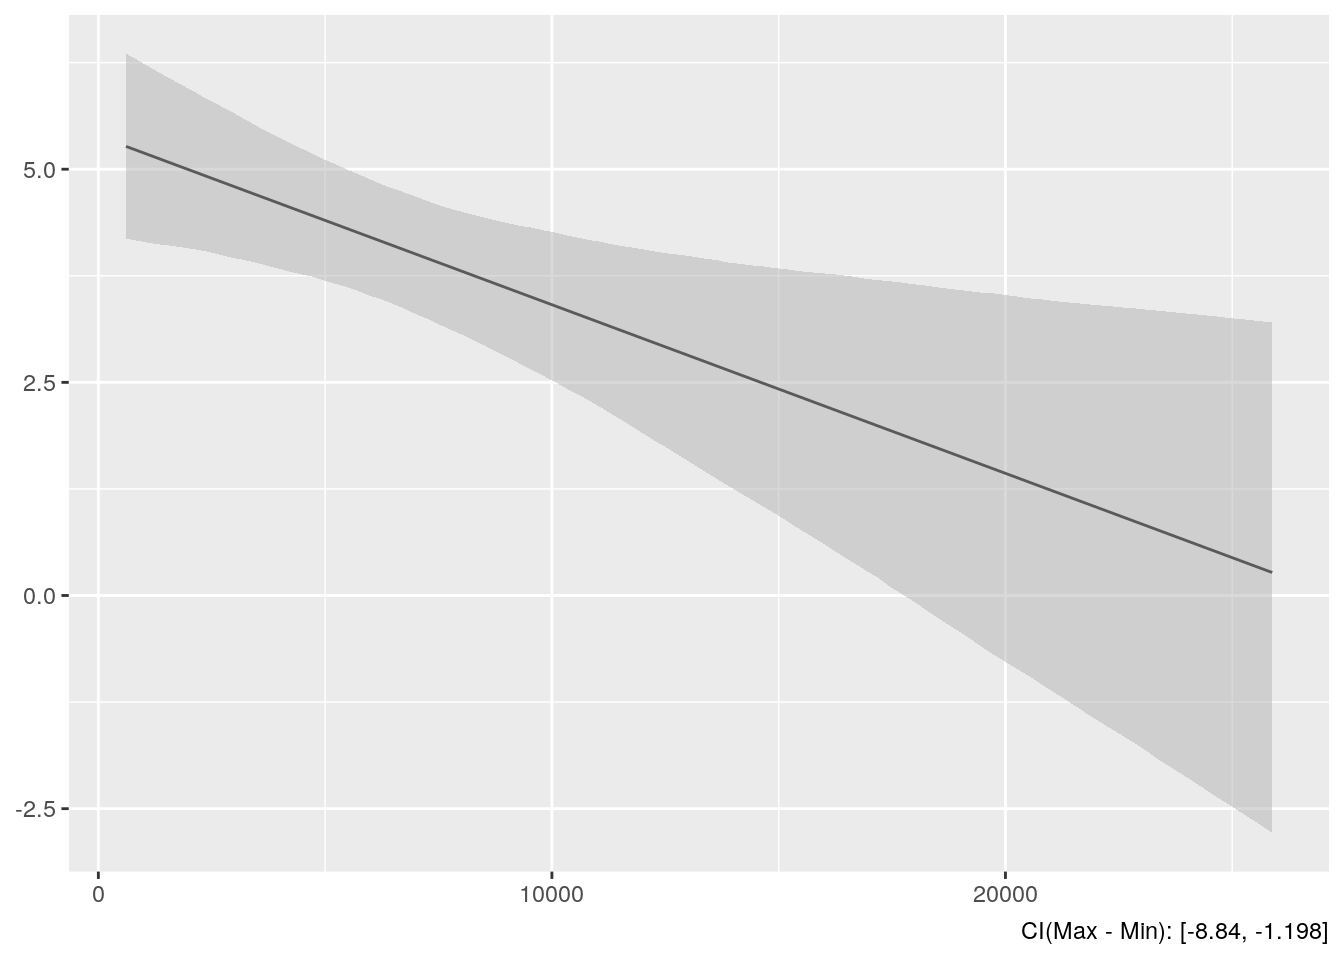
\includegraphics{pdaps_files/figure-latex/interplot-1.pdf}

We see that the marginal effect of education on prestige is high for low-income occupations, but almost nil for an occupation that earns around \$25,000/year. (The bars represent a confidence interval---of course, we haven't done any inferential statistics yet.)

\hypertarget{quadratic-and-logarithmic-models}{%
\subsection{Quadratic and Logarithmic Models}\label{quadratic-and-logarithmic-models}}

The syntax for a quadratic model is a bit weird. You would think you could use a formula like \texttt{y\ \textasciitilde{}\ x\ +\ x\^{}2}, but that won't work. Instead, you have to write \texttt{y\ \textasciitilde{}\ x\ +\ I(x\^{}2)}, as in the following example.

\begin{Shaded}
\begin{Highlighting}[]
\NormalTok{fit\_quad \textless{}{-}}\StringTok{ }\KeywordTok{lm}\NormalTok{(prestige }\OperatorTok{\textasciitilde{}}\StringTok{ }\NormalTok{education }\OperatorTok{+}\StringTok{ }\KeywordTok{I}\NormalTok{(education}\OperatorTok{\^{}}\DecValTok{2}\NormalTok{) }\OperatorTok{+}\StringTok{ }\NormalTok{income, }\DataTypeTok{data =}\NormalTok{ Prestige)}
\NormalTok{fit\_quad}
\end{Highlighting}
\end{Shaded}

\begin{verbatim}
## 
## Call:
## lm(formula = prestige ~ education + I(education^2) + income, 
##     data = Prestige)
## 
## Coefficients:
##    (Intercept)       education  I(education^2)          income  
##      10.979513        0.774768        0.153730        0.001276
\end{verbatim}

The easiest way to visualize the results of a quadratic model is to create a synthetic dataset, where you vary the relevant variable across its range while holding all the other variables fixed at the same value. Then plug the synthetic dataset into the model to get predicted values.

\begin{Shaded}
\begin{Highlighting}[]
\NormalTok{synthetic\_data \textless{}{-}}\StringTok{ }\KeywordTok{data\_frame}\NormalTok{(}
    \DataTypeTok{education =} \KeywordTok{seq}\NormalTok{(}\KeywordTok{min}\NormalTok{(Prestige}\OperatorTok{$}\NormalTok{education),}
                    \KeywordTok{max}\NormalTok{(Prestige}\OperatorTok{$}\NormalTok{education),}
                    \DataTypeTok{length.out =} \DecValTok{100}\NormalTok{),}
    \DataTypeTok{income =} \KeywordTok{mean}\NormalTok{(Prestige}\OperatorTok{$}\NormalTok{income)}
\NormalTok{)}

\NormalTok{synthetic\_data \textless{}{-}}\StringTok{ }\KeywordTok{augment}\NormalTok{(fit\_quad, }\DataTypeTok{newdata =}\NormalTok{ synthetic\_data)}
\KeywordTok{head}\NormalTok{(synthetic\_data)}
\end{Highlighting}
\end{Shaded}

\begin{verbatim}
## # A tibble: 6 x 3
##   education income .fitted
##       <dbl>  <dbl>   <dbl>
## 1      6.38  6798.    30.9
## 2      6.48  6798.    31.1
## 3      6.57  6798.    31.4
## 4      6.67  6798.    31.7
## 5      6.77  6798.    31.9
## 6      6.86  6798.    32.2
\end{verbatim}

\begin{Shaded}
\begin{Highlighting}[]
\KeywordTok{ggplot}\NormalTok{(synthetic\_data, }\KeywordTok{aes}\NormalTok{(}\DataTypeTok{x =}\NormalTok{ education, }\DataTypeTok{y =}\NormalTok{ .fitted)) }\OperatorTok{+}
\StringTok{    }\KeywordTok{geom\_line}\NormalTok{()}
\end{Highlighting}
\end{Shaded}

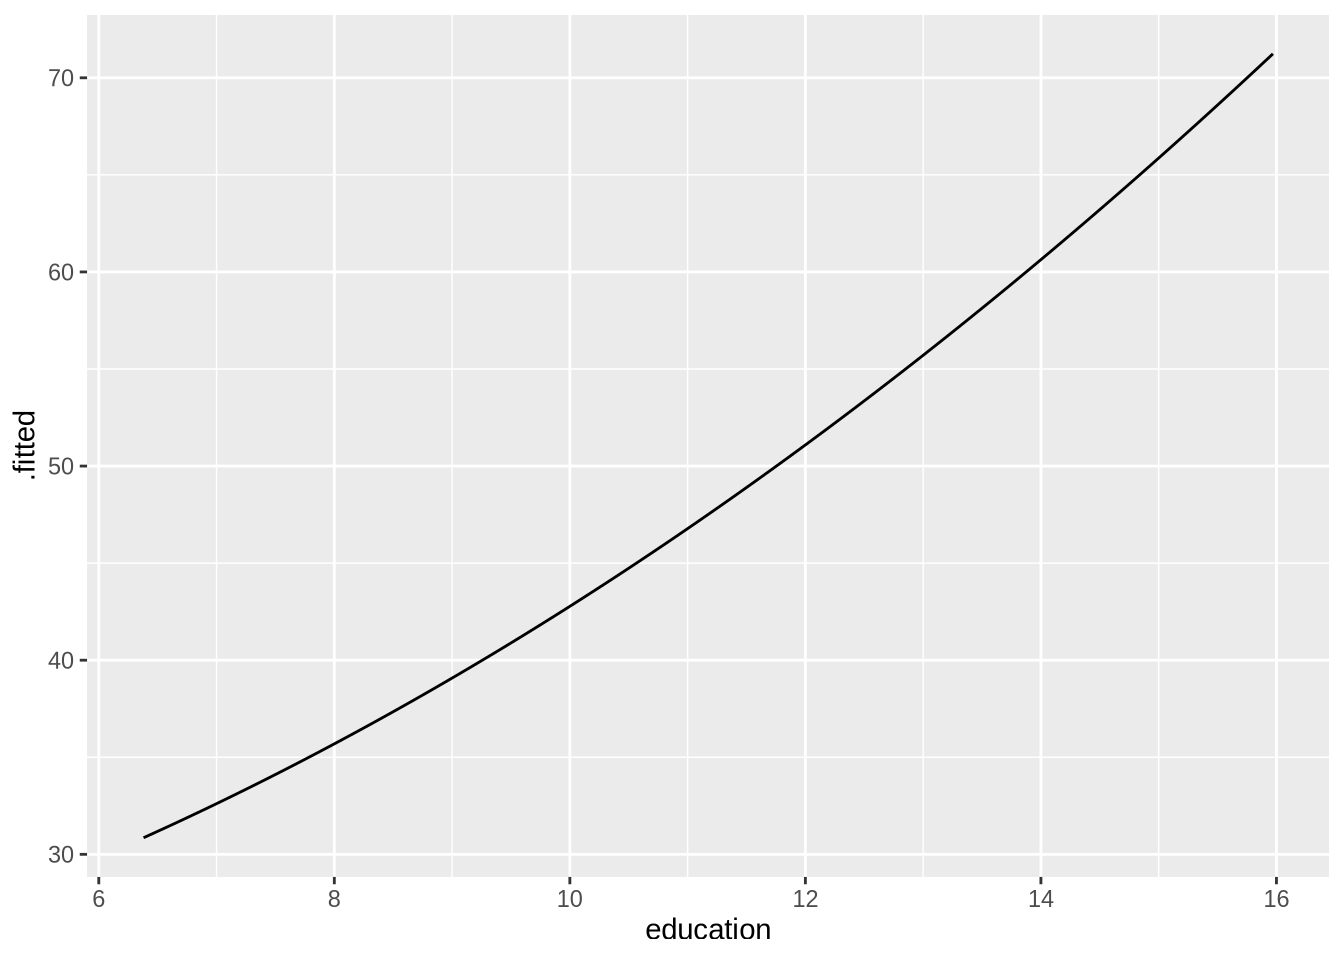
\includegraphics{pdaps_files/figure-latex/plot-quadratic-1.pdf}

In this case, within the range spanned by the sample data, the estimated quadratic relationship is only barely nonlinear.

Finally, to run a logarithmic model, just put \texttt{log()} around the variables you want to log.

\begin{Shaded}
\begin{Highlighting}[]
\NormalTok{fit\_log \textless{}{-}}\StringTok{ }\KeywordTok{lm}\NormalTok{(}\KeywordTok{log}\NormalTok{(prestige) }\OperatorTok{\textasciitilde{}}\StringTok{ }\KeywordTok{log}\NormalTok{(income) }\OperatorTok{+}\StringTok{ }\NormalTok{education, }\DataTypeTok{data =}\NormalTok{ Prestige)}
\NormalTok{fit\_log}
\end{Highlighting}
\end{Shaded}

\begin{verbatim}
## 
## Call:
## lm(formula = log(prestige) ~ log(income) + education, data = Prestige)
## 
## Coefficients:
## (Intercept)  log(income)    education  
##     0.33730      0.29912      0.07887
\end{verbatim}

To visualize the resulting relationship, you can use the same technique as for quadratic models.

\hypertarget{inference}{%
\chapter{Drawing Inferences}\label{inference}}

\providecommand{\Cov}{}
\renewcommand{\Cov}{\mathop{\rm Cov}\nolimits}
\providecommand{\SE}{}
\renewcommand{\SE}{\mathop{\rm SE}\nolimits}
\providecommand{\CI}{}
\renewcommand{\CI}{\mathop{\rm CI}\nolimits}

You can think of regression as a descriptive statistic or data reduction method---a simple way to summarize trends and relationships in multivariate data. But for better or worse, most social scientists view regression as a tool for hypothesis testing. This week, we will talk about what it is that we're doing when we gaze at the ``stars'' that accompany our regression output.

\hypertarget{the-basics-of-hypothesis-testing}{%
\section{The Basics of Hypothesis Testing}\label{the-basics-of-hypothesis-testing}}

Remember the general procedure for testing against a null hypothesis.

\begin{enumerate}
\def\labelenumi{\arabic{enumi}.}
\item
  Choose a test statistic and significance level.
\item
  Derive the sampling distribution of the test statistic under the null hypothesis.
\item
  Calculate the value of the test statistic for our sample.
\item
  Compare the sample test statistic to the sampling distribution under the null hypothesis. If the probability of obtaining a result as least as extreme as ours is at or below the significance level, reject the null hypothesis.
\end{enumerate}

Imagine the null hypothesis is true. Given that, imagine 100 labs run independent tests of the null hypothesis, each using a significance level of 0.05. If they follow the procedure above, on average 5 of the labs will reject the null hypothesis, and 95 will fail to reject the null hypothesis.

What if the null hypothesis is false? What percentage of the labs will falsely reject it? That's the \emph{power} of the test, and it depends on a number of factors: how far off the null hypothesis is, what size sample each lab is drawing, and the significance level.

Before we get into hypothesis tests for regression, let's refresh ourselves on how we draw inferences from a random sample about the population mean.

Suppose we have a sequence of \(N\) i.i.d. draws of the random variable \(X\), which we will denote \(X_1, \ldots, X_N\), and we are interested in testing the null hypothesis
\[
H_0 : E[X] = \mu_0.
\]
Let \(\bar{X}\) denote the sample mean and \(S_X\) denote the sample standard
deviation. Define the \(t\) statistic as
\[
t = \frac{\bar{X} - \mu_0}{S_X / \sqrt{N}}.
\]
The denominator of the \(t\) statistic is the \emph{standard error}---our estimate of the standard deviation of the sampling distribution under the null hypothesis. The greater the standard error, the more the statistic varies across samples, and thus the less reliable it is in any given sample. Naturally enough, our standard errors decrease with our sample size; the more data we have, the more reliably we can draw inferences.

If \(X\) is known to be normally distributed---an assumption that, in the realms political scientists deal with, is usually implausible---then the sampling distribution of \(t\) under the null hypothesis is \(t_{N - 1}\), the Student's \(t\) distribution with \(N - 1\) degrees of freedom.

If \(X\) is not known to be normally distributed, but our sample size is ``large'' (in practice, \(N \geq 30\)), we can rely on the Central Limit Theorem. As \(N \to \infty\), the distribution of \(t\) under the null hypothesis is approximately \(N(0, 1)\), the normal distribution with mean zero and variance one.

\hypertarget{variance-of-ols}{%
\section{Variance of OLS}\label{variance-of-ols}}

Now let us return to the world of the linear model,
\[
\mathbf{Y} = \mathbf{X} \beta + \epsilon,
\]
and the OLS estimator of \(\beta\),
\[
\hat{\beta}_{\text{OLS}} = (\mathbf{X}^\top \mathbf{X})^{-1} \mathbf{X}^\top \mathbf{Y}.
\]
In order to draw inferences on OLS results, the first thing we need to know is the variance of the OLS estimator. You will remember from Stat 1 that the variance of the sample mean, \(\bar{X}\), is
\[
V[\bar{X}] = \frac{V[X]}{N},
\]
whose square root ends up in the denominator of the \(t\)-test statistic. We will do something similar for OLS.

Throughout this week, we will maintain the following two assumptions on the error term:

\begin{itemize}
\item
  Strict exogeneity: \(E[\epsilon \,|\, \mathbf{X}] = \mathbf{0}\).
\item
  Spherical errors: \(V[\epsilon \,|\, \mathbf{X}] = \sigma^2 \mathbf{I}_N\), where \(\sigma^2 > 0\).
\end{itemize}

Without the first assumption, OLS is hopeless to begin with. Without the second assumption, OLS is unbiased and consistent, but not efficient. Later on, we will discuss how to draw inferences in the presence of non-spherical errors.

The OLS estimator is a \(K \times 1\) vector, so its variance won't be a single number---it will be a \(K \times K\) matrix,
\[
V[\hat{\beta}] = \begin{bmatrix}
  V[\hat{\beta}_1] & \mathop{\rm Cov}\nolimits[\hat{\beta}_1, \hat{\beta}_2] & \cdots & \mathop{\rm Cov}\nolimits[\hat{\beta}_1, \hat{\beta}_K] \\
  \mathop{\rm Cov}\nolimits[\hat{\beta}_2, \hat{\beta}_1] & V[\hat{\beta}_2] & \cdots & \mathop{\rm Cov}\nolimits[\hat{\beta}_2, \hat{\beta}_K] \\
  \vdots & \vdots & \ddots & \vdots \\
  \mathop{\rm Cov}\nolimits[\hat{\beta}_K, \hat{\beta}_1] & \mathop{\rm Cov}\nolimits[\hat{\beta}_K, \hat{\beta}_2] & \cdots & V[\hat{\beta}_K] \\
\end{bmatrix}.
\]
Specifically, the variance of the OLS estimator (treating the covariates as fixed) is
\[
V[\hat{\beta} \,|\, \mathbf{X}] = \sigma^2 (\mathbf{X}^\top \mathbf{X})^{-1}.
\]
See the appendix to this chapter---or any graduate-level econometrics textbook---for how we derive this result.

If we knew \(\sigma^2\), the variance of the error term, then we could just use the above formula to draw inferences. Realistically, though, we will need to estimate \(\sigma^2\). We will do so using the residual variance,
\[
\hat{\sigma}^2
= \frac{\sum_n (Y_n - \mathbf{x}_n \cdot \hat{\beta})^2}{N - K}
= \frac{\text{SSE}}{N - K}.
\]
Why do we divide by \(N - K\)? Remember that when we estimate the variance of a random variable, we divide the squared deviations from the mean by \(N - 1\) to correct for the degree of freedom we used to estimate the sample mean. The resulting estimator is unbiased. Similarly, when estimating the residual variance of a linear regression model, we need to correct for the \(K\) degrees of freedom we used to estimate the model coefficients. Hence we must divide by \(N - K\) in order for \(\hat{\sigma}^2\) to be unbiased.

Under the spherical error assumption, our estimate of the variance of OLS will therefore be the \(K \times K\) matrix
\[
\hat{\Sigma} = \hat{\sigma}^2 (\mathbf{X}^\top \mathbf{X})^{-1}.
\]
A very important note. If the errors are not spherical, this formula produces a \emph{biased} and \emph{inconsistent} estimate of the sampling variability of OLS. This is true even though the OLS estimate itself is unbiased and consistent. In other words, if we use OLS in the presence of non-spherical errors:

\begin{itemize}
\item
  Our estimates will not be systematically biased away from the population parameter, and the probability of our estimate being any meaningful distance away from the population parameter goes to zero as our sample size increases.
\item
  Our hypothesis tests will \textbf{not} perform as advertised---typically, they will lead us to reject the null hypothesis more often than we should---and this problem does \textbf{not} go away as our sample size increases.
\end{itemize}

For the remainder of this week, we will proceed under the assumption of spherical errors. Later on, we will discuss how to draw inferences appropriately when this assumption fails to hold.

\hypertarget{single-variable-hypotheses}{%
\section{Single Variable Hypotheses}\label{single-variable-hypotheses}}

Consider a null hypothesis about the population value of a single coefficient, of the form
\[
H_0 : \beta_k = b,
\]
where \(b\) is a fixed constant. Usually, though not always, political scientists concern themselves with null hypotheses of the form \(\beta_k = 0\); i.e., the \(k\)'th variable has zero (so-called) marginal effect on the response.

We will test this hypothesis using the familiar \(t\)-statistic. The \emph{estimated standard error} of \(\hat{\beta}_k\) is
\[
\mathop{\rm SE}\nolimits(\hat{\beta}_k) = \sqrt{\hat{\Sigma}_{kk}},
\]
where \(\hat{\Sigma}_{kk}\) denotes the \(k\)'th element of the diagonal of \(\hat{\Sigma} = \hat{\sigma}^2 (\mathbf{X}^\top \mathbf{X})^{-1}\). The ``standard errors'' that appear alongside your regression output are calculating by taking the square root of the diagonal of this matrix.

The \(t\) statistic for the test of the null hypothesis \(H_0\) is in the familiar ``estimate divided by standard error'' form,
\[
t = \frac{\hat{\beta}_k - b}{\mathop{\rm SE}\nolimits(\hat{\beta}_k)} = \frac{\hat{\beta}_k - b}{\sqrt{\hat{\Sigma}_{kk}}}.
\]
Our mode of inference from there depends on the sample size and on whether we are willing to make a normality assumption.

\begin{itemize}
\item
  If \(\epsilon\) is normally distributed, then the sampling distribution of our test statistic is \(t_{N - K}\), the \(t\) distribution with \(N - K\) degrees of freedom.
\item
  As our sample size grows large, the sampling distribution of our test statistic is approximately \(N(0, 1)\), the normal distribution with mean zero and variance one. This follows from the Central Limit Theorem, and it holds even if \(\epsilon\) is \emph{not} normally distributed.
\end{itemize}

So if you have a small sample, the validity of the standard hypothesis test depends on a normality assumption that may or may not be palatable, depending on the circumstances. Other techniques exist for this situation, but they are beyond the scope of this course. Of course, if your sample is so small that you need to resort to non-standard hypothesis testing techniques in order to draw appropriate inferences, you should probably go back to the drawing board on your study design.

Regardless of your sample size, regression software will compare your test statistics to \(t_{N - K}\) to calculate \(p\)-values and the results of hypothesis tests. This is innocuous even if you don't assume normality, since if \(N\) is large the \(t_{N - K}\) distribution is approximately the same as the \(N(0, 1)\) distribution (with infinitesimally fatter tails).

Our method of constructing confidence intervals for a single parameter is also analogous to what we do with the sample mean. Let \(z_{\alpha}\) be the critical value of the sampling distribution of our test statistic for our chosen significance level \(\alpha\). For example, the critical value of \(N(0, 1)\) for significance \(\alpha = 0.05\) is \(z_{\alpha} = 1.96\). Then the \((1 - \alpha)\)-confidence interval around \(\hat{\beta}_k\) is
\[
\mathop{\rm CI}\nolimits_{1 - \alpha}(\hat{\beta}_k) = [\hat{\beta}_k - z_{\alpha} \mathop{\rm SE}\nolimits(\hat{\beta}_k), \hat{\beta}_k + z_{\alpha} \mathop{\rm SE}\nolimits(\hat{\beta}_k)].
\]

\hypertarget{multiple-variable-hypotheses}{%
\section{Multiple Variable Hypotheses}\label{multiple-variable-hypotheses}}

It is common, especially (though not exclusively) when working with categorical variables or higher-order terms, to have hypotheses involving multiple variables. For example, think of our model from last week,
\[
\text{Trump}_n = \beta_1 + \beta_2 \text{Independent}_n + \beta_3 \text{Democratic}_n + \beta_4 \text{Age}_n + \epsilon_n.
\]
Remember that \(\beta_2\) denotes the expected difference between Independents and Republicans (the omitted category) of the same age in their propensity to vote for Trump, and \(\beta_3\) denotes the expected difference between Democrats and Republicans of the same age.

If our null hypothesis were that Independents and Republicans of the same age had the same chance of voting for Trump, we would state that as
\[
H_0 : \beta_2 = 0.
\]
But what about the null hypothesis were that Independents and Democrats had the same chance of voting for Trump? We would have to phrase that in terms of multiple coefficients,
\[
H_0 : \beta_2 = \beta_3,
\]
or equivalently,
\[
H_0 : \beta_2 - \beta_3 = 0.
\]
Or what if our null hypothesis were that party identification made no difference at all? That would mean Independents and Democrats are both no different than Republicans on average, or in our model notation,
\[
H_0 : \left\{ \begin{aligned}
\beta_2 &= 0, \\
\beta_3 &= 0.
\end{aligned} \right.
\]

Each of these, including the simple single-variable hypothesis, is a linear system in \(\beta\). In other words, we can write each of these hypotheses in the form
\[
H_0 : \mathbf{R} \beta - \mathbf{c} = \mathbf{0},
\]
where \(\mathbf{R}\) is a fixed \(r \times K\) matrix (where \(r\) is the number of restrictions we intend to test) and \(\mathbf{c}\) is a fixed \(r \times 1\) vector.

Perhaps the easiest way to test a hypothesis of this form is the \emph{Wald test}. We form the test statistic
\[
W = (\mathbf{R} \beta - \mathbf{c})^\top  (\mathbf{R} \hat{\Sigma} \mathbf{R}^\top)^{-1} (\mathbf{R} \beta - \mathbf{c}),
\]
which, despite all the matrices involved, works out to be a scalar. Under \(H_0\), the asymptotic sampling distribution of \(W\) is \(\chi^2_r\), the chi-squared distribution with \(r\) degrees of freedom.\footnote{You will notice that, for a single-variable hypothesis \(H_0 : \beta_k = b\), the Wald statistic reduces to the square of the \(t\) statistic. Since the asymptotic distribution of the \(t\) statistic is standard normal under the null hypothesis, it follows that the asymptotic distribution of its square is \(\chi^2_1\) under the null hypothesis.} Regression software like R will usually report an \(F\) statistic, since the exact (not asymptotic) distribution of \(W\) follows an \(F\) distribution in the special case of normal residual error.

The Wald test is not just an aggregation of the individual \(t\) tests of the coefficients. Two coefficients might each individually be statistically insignificant, yet the Wald test may lead us to reject the null hypothesis that both are zero. Conversely, one of a group of coefficients might be statistically significant, and yet the Wald test may not have us reject the null hypothesis that all are zero.

We already saw a couple of examples of how to use the Wald test with a model with a categorical variable. Let's also quickly consider its use in some other models with less-common specifications.

Imagine an interactive model,
\[
Y_n = \beta_1 + \beta_2 X_n + \beta_3 Z_n + \beta_4 (X_n \times Z_n) + \epsilon_n.
\]
The interaction term captures how the (so-called) marginal effect of \(X_n\) depends on the value of \(Z_n\), and vice versa. If your null hypothesis is that the marginal effect of \(X_n\) does not depend on \(Z_n\), you could use perform a \(t\) test of
\[
H_0 : \beta_4 = 0.
\]
But what if your null hypothesis is that the marginal effect of \(X_n\) is \emph{always} zero, regardless of the value of \(Z_n\)? Some people make the unfortunate mistake of testing this via the null hypothesis
\[
H_0 : \beta_2 = 0,
\]
but that only means the marginal effect of \(X_n\) is zero \emph{when \(Z_n = 0\)}. What you want is the composite null
\[
H_0 : \left\{ \begin{aligned}
  \beta_2 &= 0, \\
  \beta_4 &= 0,
\end{aligned} \right.
\]
or, in matrix form,
\[
\begin{bmatrix}
  0 & 1 & 0 & 0 \\
  0 & 0 & 0 & 1
\end{bmatrix}
\begin{bmatrix}
  \beta_1 \\ \beta_2 \\ \beta_3 \\ \beta_4
\end{bmatrix}
=
\begin{bmatrix}
  0 \\ 0
\end{bmatrix}.
\]

Similarly, think of the quadratic model,
\[
Y_n = \beta_1 + \beta_2 X_n + \beta_3 X_n^2 + \epsilon_n.
\]
The null hypothesis that the (so-called) marginal effect of \(X_n\) is constant is equivalent to
\[
H_0 : \beta_3 = 0.
\]
But if we wanted to test against the null hypothesis that the marginal effect of \(X_n\) is \emph{always} zero, we would have to use a composite null,
\[
H_0 : \left\{ \begin{aligned}
  \beta_2 &= 0, \\
  \beta_3 &= 0.
\end{aligned} \right.
\]

\hypertarget{appendix-full-derivation-of-ols-variance}{%
\section{Appendix: Full Derivation of OLS Variance}\label{appendix-full-derivation-of-ols-variance}}

We will assume strict exogeneity,
\[
E [\epsilon \,|\, \mathbf{X}] = \mathbf{0},
\]
and spherical errors,
\[
V [\epsilon \,|\, \mathbf{X}] = E [\epsilon \epsilon^\top \,|\, \mathbf{X}] = \sigma^2 \mathbf{I}.
\]
A useful thing to know is that since \(\mathbf{X}^\top \mathbf{X}\) is symmetric, so is its inverse:
\[
[(\mathbf{X}^\top \mathbf{X})^{-1}]^\top = (\mathbf{X}^\top \mathbf{X})^{-1}.
\]

Let's start by deriving the variance from our formula for a vector-valued random variable,
\[
V[C] = E \left[ (C - E[C]) (C - E[C])^\top \right].
\]
For the OLS estimator \(\hat{\beta}\), we have
\[
\begin{aligned}
  V[\hat{\beta} \,|\, \mathbf{X}]
  &= E \left[ \left(\hat{\beta} - E[\hat{\beta}]\right) \left(\hat{\beta} - E[\hat{\beta}]\right)^\top \,|\, \mathbf{X} \right] \\
  &= E \left[ \left(\hat{\beta} - \beta\right) \left(\hat{\beta} - \beta\right)^\top \,|\, \mathbf{X} \right] \\
  &= E \left[ \hat{\beta} \hat{\beta}^\top - 2 \beta \hat{\beta}^\top + \beta \beta^\top \,|\, \mathbf{X} \right] \\
  &= E \left[ \hat{\beta} \hat{\beta}^\top \,|\, \mathbf{X} \right] - 2 \beta E \left[ \hat{\beta}^\top \,|\, \mathbf{X} \right] + \beta \beta^\top \\
  &= E \left[ (\mathbf{X}^\top \mathbf{X})^{-1} \mathbf{X}^\top \mathbf{Y} \mathbf{Y}^\top \mathbf{X} (\mathbf{X}^\top \mathbf{X})^{-1} \,|\, \mathbf{X} \right] - \beta \beta^\top \\
  &= (\mathbf{X}^\top \mathbf{X})^{-1} \mathbf{X}^\top E \left[ \mathbf{Y} \mathbf{Y}^\top \,|\, \mathbf{X} \right] \mathbf{X} (\mathbf{X}^\top \mathbf{X})^{-1} - \beta \beta^\top.
\end{aligned}
\]
Since \(\mathbf{Y} = \mathbf{X} \beta + \epsilon\), we have
\[
\begin{aligned}
  E \left[ \mathbf{Y} \mathbf{Y}^\top \,|\, \mathbf{X} \right]
  &= E \left[ (\mathbf{X} \beta + \epsilon) (\mathbf{X} \beta + \epsilon)^\top \,|\, \mathbf{X} \right] \\
  &= E \left[ \mathbf{X} \beta \beta^\top \mathbf{X}^\top + 2 \epsilon \beta^\top \mathbf{X}^\top + \epsilon \epsilon^\top \,|\, \mathbf{X} \right] \\
  &= \mathbf{X} \beta \beta^\top \mathbf{X}^\top + 2 \underbrace{E[\epsilon \,|\, \mathbf{X}]}_{= \mathbf{0}} \beta^\top \mathbf{X}^\top + E[\epsilon \epsilon^\top \,|\, \mathbf{X}] \\
  &= \mathbf{X} \beta \beta^\top \mathbf{X}^\top + \sigma^2 \mathbf{I}.
\end{aligned}
\]
Continuing from above, we have
\[
\begin{aligned}
  V[\hat{\beta} \,|\, \mathbf{X}]
  &= (\mathbf{X}^\top \mathbf{X})^{-1} \mathbf{X}^\top E \left[ \mathbf{Y} \mathbf{Y}^\top \,|\, \mathbf{X} \right] \mathbf{X} (\mathbf{X}^\top \mathbf{X})^{-1} - \beta \beta^\top \\
  &= (\mathbf{X}^\top \mathbf{X})^{-1} \mathbf{X}^\top ( \mathbf{X} \beta \beta^\top \mathbf{X}^\top + \sigma^2 \mathbf{I} ) \mathbf{X} (\mathbf{X}^\top \mathbf{X})^{-1} - \beta \beta^\top \\
  &= (\mathbf{X}^\top \mathbf{X})^{-1} (\mathbf{X}^\top \mathbf{X}) \beta \beta^\top (\mathbf{X}^\top \mathbf{X}) (\mathbf{X}^\top \mathbf{X})^{-1} \\ &\quad + \sigma^2 (\mathbf{X}^\top \mathbf{X})^{-1} \mathbf{X}^\top \mathbf{X} (\mathbf{X}^\top \mathbf{X})^{-1} - \beta \beta^\top \\
  &= \beta \beta^\top + \sigma^2 (\mathbf{X}^\top \mathbf{X})^{-1} - \beta \beta^\top \\
  &= \sigma^2 (\mathbf{X}^\top \mathbf{X})^{-1}.
\end{aligned}
\]

A slightly easier way to get there would be to apply two of the helpful properties of variance. You'll remember from the study of scalar-valued random variables that, for a random variable \(A\) and scalars \(c\) and \(d\),
\[
\begin{aligned}
  V[c A] &= c^2 V[A], \\
  V[A + d] &= V[A].
\end{aligned}
\]
Similarly, for an \(m \times 1\) vector random variable \(\mathbf{A}\), a fixed \(n \times m\) matrix \(\mathbf{C}\), and a fixed \(m \times 1\) vector \(\mathbf{d}\), we have
\[
\begin{aligned}
  V[\mathbf{C} \mathbf{A}] &= \mathbf{C} V[\mathbf{A}] \mathbf{C}^\top, \\
  V[\mathbf{A} + \mathbf{d}] &= V[\mathbf{A}].
\end{aligned}
\]
Consequently,
\[
\begin{aligned}
  V \left[ \hat{\beta} \,|\, \mathbf{X} \right]
  &= V[ (\mathbf{X}^\top \mathbf{X})^{-1} \mathbf{X}^\top \mathbf{Y} \,|\, \mathbf{X} ] \\
  &= (\mathbf{X}^\top \mathbf{X})^{-1} \mathbf{X}^\top V [\mathbf{Y} \,|\, \mathbf{X}] \mathbf{X} (\mathbf{X}^\top \mathbf{X})^{-1} \\
  &= (\mathbf{X}^\top \mathbf{X})^{-1} \mathbf{X}^\top V [\mathbf{X} \beta + \epsilon \,|\, \mathbf{X}] \mathbf{X} (\mathbf{X}^\top \mathbf{X})^{-1} \\
  &= (\mathbf{X}^\top \mathbf{X})^{-1} \mathbf{X}^\top V [\epsilon \,|\, \mathbf{X}] \mathbf{X} (\mathbf{X}^\top \mathbf{X})^{-1} \\
  &= (\mathbf{X}^\top \mathbf{X})^{-1} \mathbf{X}^\top (\sigma^2 \mathbf{I}) \mathbf{X} (\mathbf{X}^\top \mathbf{X})^{-1} \\
  &= \sigma^2 (\mathbf{X}^\top \mathbf{X})^{-1}.
\end{aligned}
\]

\hypertarget{appendix-regression-inference-in-r}{%
\section{Appendix: Regression Inference in R}\label{appendix-regression-inference-in-r}}

As usual, we will rely on the \textbf{tidyverse} and \textbf{broom} packages. We will also be using the \textbf{car} package, not only for data but also for its hypothesis testing functions.

\begin{Shaded}
\begin{Highlighting}[]
\KeywordTok{library}\NormalTok{(}\StringTok{"tidyverse"}\NormalTok{)}
\KeywordTok{library}\NormalTok{(}\StringTok{"broom"}\NormalTok{)}
\KeywordTok{library}\NormalTok{(}\StringTok{"car"}\NormalTok{)}
\end{Highlighting}
\end{Shaded}

Using the \texttt{Prestige} data, let us regress occupational prestige on the type of occupation (blue collar, white collar, or professional) and its average income and education.

\begin{Shaded}
\begin{Highlighting}[]
\KeywordTok{data}\NormalTok{(}\StringTok{"Prestige"}\NormalTok{, }\DataTypeTok{package =} \StringTok{"carData"}\NormalTok{)}
\NormalTok{fit \textless{}{-}}\StringTok{ }\KeywordTok{lm}\NormalTok{(prestige }\OperatorTok{\textasciitilde{}}\StringTok{ }\NormalTok{type }\OperatorTok{+}\StringTok{ }\NormalTok{education }\OperatorTok{+}\StringTok{ }\NormalTok{income, }\DataTypeTok{data =}\NormalTok{ Prestige)}
\end{Highlighting}
\end{Shaded}

\texttt{summary()} prints the ``regression table'' containing the following information:

\begin{itemize}
\tightlist
\item
  Estimate of each coefficient.
\item
  Estimated standard error of each coefficient estimate.
\item
  \(t\) statistic for each coefficient estimate, for the test against the null hypothesis that the population value of the corresponding coefficient is zero (\(H_0 : \beta_k = 0\)).
\item
  \(p\) value (two-tailed)\footnote{One-tailed tests, while unproblematic in theory, in practice are usually a signal that the two-tailed test was insignificant and the author is fudging it. Don't send a bad signal; always use two-tailed tests.} for the aforementioned hypothesis test.
\end{itemize}

\begin{Shaded}
\begin{Highlighting}[]
\KeywordTok{summary}\NormalTok{(fit)}
\end{Highlighting}
\end{Shaded}

\begin{verbatim}
## 
## Call:
## lm(formula = prestige ~ type + education + income, data = Prestige)
## 
## Residuals:
##      Min       1Q   Median       3Q      Max 
## -14.9529  -4.4486   0.1678   5.0566  18.6320 
## 
## Coefficients:
##               Estimate Std. Error t value Pr(>|t|)    
## (Intercept) -0.6229292  5.2275255  -0.119    0.905    
## typeprof     6.0389707  3.8668551   1.562    0.122    
## typewc      -2.7372307  2.5139324  -1.089    0.279    
## education    3.6731661  0.6405016   5.735 1.21e-07 ***
## income       0.0010132  0.0002209   4.586 1.40e-05 ***
## ---
## Signif. codes:  0 '***' 0.001 '**' 0.01 '*' 0.05 '.' 0.1 ' ' 1
## 
## Residual standard error: 7.095 on 93 degrees of freedom
##   (4 observations deleted due to missingness)
## Multiple R-squared:  0.8349, Adjusted R-squared:  0.8278 
## F-statistic: 117.5 on 4 and 93 DF,  p-value: < 2.2e-16
\end{verbatim}

This is useful for a quick check on the output, but not so much if you want to use the standard errors for further calculations (e.g., making a plot). To extract the standard errors, use the \texttt{tidy()} function from \textbf{broom}. This returns a data frame whose columns correspond to the \texttt{summary()} output.

\begin{Shaded}
\begin{Highlighting}[]
\NormalTok{fit\_results \textless{}{-}}\StringTok{ }\KeywordTok{tidy}\NormalTok{(fit)}
\NormalTok{fit\_results}
\end{Highlighting}
\end{Shaded}

\begin{verbatim}
## # A tibble: 5 x 5
##   term        estimate std.error statistic     p.value
##   <chr>          <dbl>     <dbl>     <dbl>       <dbl>
## 1 (Intercept) -0.623    5.23        -0.119 0.905      
## 2 typeprof     6.04     3.87         1.56  0.122      
## 3 typewc      -2.74     2.51        -1.09  0.279      
## 4 education    3.67     0.641        5.73  0.000000121
## 5 income       0.00101  0.000221     4.59  0.0000140
\end{verbatim}

\begin{Shaded}
\begin{Highlighting}[]
\NormalTok{fit\_results}\OperatorTok{$}\NormalTok{std.error}
\end{Highlighting}
\end{Shaded}

\begin{verbatim}
## [1] 5.2275254877 3.8668550979 2.5139324035 0.6405016204 0.0002209185
\end{verbatim}

To extract the full (estimated) variance matrix, use the \texttt{vcov()} function.

\begin{Shaded}
\begin{Highlighting}[]
\KeywordTok{vcov}\NormalTok{(fit)}
\end{Highlighting}
\end{Shaded}

\begin{verbatim}
##               (Intercept)      typeprof        typewc     education
## (Intercept)  2.732702e+01  1.663699e+01  7.3984873320 -3.196460e+00
## typeprof     1.663699e+01  1.495257e+01  6.7970730800 -2.123883e+00
## typewc       7.398487e+00  6.797073e+00  6.3198561295 -1.106184e+00
## education   -3.196460e+00 -2.123883e+00 -1.1061842075  4.102423e-01
## income       9.996273e-05 -4.984256e-06  0.0001310818 -4.333455e-05
##                    income
## (Intercept)  9.996273e-05
## typeprof    -4.984256e-06
## typewc       1.310818e-04
## education   -4.333455e-05
## income       4.880497e-08
\end{verbatim}

Luckily, you shouldn't often need to extract the individual standard errors or the variance matrix. R has convenience functions to perform most of the calculations you would care about.

To obtain confidence intervals for the regression coefficients, use the \texttt{confint()} function.

\begin{Shaded}
\begin{Highlighting}[]
\KeywordTok{confint}\NormalTok{(fit)}
\end{Highlighting}
\end{Shaded}

\begin{verbatim}
##                     2.5 %       97.5 %
## (Intercept) -1.100376e+01  9.757900433
## typeprof    -1.639837e+00 13.717778520
## typewc      -7.729402e+00  2.254940810
## education    2.401257e+00  4.945075332
## income       5.744929e-04  0.001451893
\end{verbatim}

\begin{Shaded}
\begin{Highlighting}[]
\KeywordTok{confint}\NormalTok{(fit, }\DataTypeTok{level =} \FloatTok{0.99}\NormalTok{)  }\CommentTok{\# Changing the confidence level}
\end{Highlighting}
\end{Shaded}

\begin{verbatim}
##                     0.5 %      99.5 %
## (Intercept) -1.436992e+01 13.12406265
## typeprof    -4.129823e+00 16.20776380
## typewc      -9.348200e+00  3.87373813
## education    1.988818e+00  5.35751375
## income       4.322368e-04  0.00159415
\end{verbatim}

\begin{Shaded}
\begin{Highlighting}[]
\KeywordTok{confint}\NormalTok{(fit, }\StringTok{"education"}\NormalTok{)   }\CommentTok{\# Only for one coefficient}
\end{Highlighting}
\end{Shaded}

\begin{verbatim}
##              2.5 %   97.5 %
## education 2.401257 4.945075
\end{verbatim}

You may also be interested in testing against null hypotheses other than each individual coefficient being zero. This is where the \texttt{linearHypothesis()} function from the car package comes in. For example, suppose we wanted to test against the null hypothesis that the population coefficient on education is 3.

\begin{Shaded}
\begin{Highlighting}[]
\KeywordTok{linearHypothesis}\NormalTok{(fit, }\StringTok{"education = 3"}\NormalTok{)}
\end{Highlighting}
\end{Shaded}

\begin{verbatim}
## Linear hypothesis test
## 
## Hypothesis:
## education = 3
## 
## Model 1: restricted model
## Model 2: prestige ~ type + education + income
## 
##   Res.Df    RSS Df Sum of Sq      F Pr(>F)
## 1     94 4736.9                           
## 2     93 4681.3  1    55.601 1.1046  0.296
\end{verbatim}

We care about the last two columns of the bottom row. \texttt{F} gives us the test statistic,\footnote{Why an \(F\) statistic instead of a \(t\) statistic? If the random variable \(Z\) has a \(t\) distribution with \(n\) degrees of freedom, then \(Z^2\) has an \(F\) distribution with \(1,n\) degrees of freedom. The \(F\) statistic generalizes better to the case of multiple hypotheses.} and \texttt{Pr(\textgreater{}F)} gives us the associated \(p\)-value. Here our \(p\)-value is 0.3, so we wouldn't reject the null hypothesis that the population coefficient on education is 3.

Two quick notes on the \texttt{linearHypothesis()} function:

\begin{itemize}
\item
  Make sure to place your hypothesis in quotes. (Or if you have multiple hypotheses, that you use a vector of quoted strings.) The function will not work if you run something like \texttt{linearHypothesis(fit,\ education\ =\ 3)}.
\item
  Make sure the name of the coefficient(s) you're testing are exactly the same as in the regression output. This requires particular care when you're dealing with factor variables, interactions, or quadratic terms.
\end{itemize}

Of course, for a univariate hypothesis test like this one, we could have just used the confidence interval to figure out the answer. The real value of \texttt{linearHypothesis()} comes in simultaneously testing hypotheses about multiple coefficients---i.e., the Wald test.

For example, let's test the null hypothesis that the population coefficients on white-collar and professional are the same.

\begin{Shaded}
\begin{Highlighting}[]
\KeywordTok{linearHypothesis}\NormalTok{(fit, }\StringTok{"typewc = typeprof"}\NormalTok{)}
\end{Highlighting}
\end{Shaded}

\begin{verbatim}
## Linear hypothesis test
## 
## Hypothesis:
## - typeprof  + typewc = 0
## 
## Model 1: restricted model
## Model 2: prestige ~ type + education + income
## 
##   Res.Df    RSS Df Sum of Sq      F   Pr(>F)   
## 1     94 5186.2                                
## 2     93 4681.3  1    504.93 10.031 0.002082 **
## ---
## Signif. codes:  0 '***' 0.001 '**' 0.01 '*' 0.05 '.' 0.1 ' ' 1
\end{verbatim}

We would reject this null hypothesis except under particularly stringent significance levels (less than 0.002).

What about the composite hypothesis that the population coefficients on white-collar and professional both equal zero? To test this, we pass a \emph{vector} of hypotheses.

\begin{Shaded}
\begin{Highlighting}[]
\KeywordTok{linearHypothesis}\NormalTok{(fit, }\KeywordTok{c}\NormalTok{(}\StringTok{"typewc = 0"}\NormalTok{, }\StringTok{"typeprof = 0"}\NormalTok{))}
\end{Highlighting}
\end{Shaded}

\begin{verbatim}
## Linear hypothesis test
## 
## Hypothesis:
## typewc = 0
## typeprof = 0
## 
## Model 1: restricted model
## Model 2: prestige ~ type + education + income
## 
##   Res.Df    RSS Df Sum of Sq      F   Pr(>F)   
## 1     95 5272.4                                
## 2     93 4681.3  2    591.16 5.8721 0.003966 **
## ---
## Signif. codes:  0 '***' 0.001 '**' 0.01 '*' 0.05 '.' 0.1 ' ' 1
\end{verbatim}

The \(p\)-value corresponding to this hypothesis test is 0.004. This illustrates a key feature of composite hypothesis tests. You'll remember from the original regression output that neither of the occupational indicators were significant on their own.

\begin{Shaded}
\begin{Highlighting}[]
\KeywordTok{summary}\NormalTok{(fit)}
\end{Highlighting}
\end{Shaded}

\begin{verbatim}
## 
## Call:
## lm(formula = prestige ~ type + education + income, data = Prestige)
## 
## Residuals:
##      Min       1Q   Median       3Q      Max 
## -14.9529  -4.4486   0.1678   5.0566  18.6320 
## 
## Coefficients:
##               Estimate Std. Error t value Pr(>|t|)    
## (Intercept) -0.6229292  5.2275255  -0.119    0.905    
## typeprof     6.0389707  3.8668551   1.562    0.122    
## typewc      -2.7372307  2.5139324  -1.089    0.279    
## education    3.6731661  0.6405016   5.735 1.21e-07 ***
## income       0.0010132  0.0002209   4.586 1.40e-05 ***
## ---
## Signif. codes:  0 '***' 0.001 '**' 0.01 '*' 0.05 '.' 0.1 ' ' 1
## 
## Residual standard error: 7.095 on 93 degrees of freedom
##   (4 observations deleted due to missingness)
## Multiple R-squared:  0.8349, Adjusted R-squared:  0.8278 
## F-statistic: 117.5 on 4 and 93 DF,  p-value: < 2.2e-16
\end{verbatim}

So, operating at conventional significant levels, we would:

\begin{itemize}
\tightlist
\item
  Fail to reject the null that the coefficient on professional is zero
\item
  Fail to reject the null that the coefficient on white-collar is zero
\item
  Reject the null that the coefficients on both are zero
\end{itemize}

This seems contradictory, but it just illustrates the limits of drawing inferences from a finite sample. What the results of these hypothesis tests are telling us is that we have enough information to conclude that there are differences in prestige across occupational categories, holding average education and income fixed. However, we do not have enough information to identify exactly where those differences are coming---i.e., exactly which of the two categories it is that differs from the omitted baseline.

\hypertarget{nonspherical}{%
\chapter{Non-Spherical Errors}\label{nonspherical}}

In our consideration so far of the linear model,
\[
\mathbf{Y} = \mathbf{X} \beta + \epsilon,
\]
we have focused on the ordinary least squares estimator,
\[
\hat{\beta}_{\text{OLS}} = (\mathbf{X}^\top \mathbf{X})^{-1} \mathbf{X}^\top \mathbf{Y}.
\]
We have seen that OLS is an unbiased and consistent estimator of the linear model parameters as long as we have strict exogeneity,
\[
E[\epsilon \,|\, \mathbf{X}] = \mathbf{0}.
\]
However, two more important properties of OLS depend on the assumption of spherical errors,
\[
V[\epsilon \,|\, \mathbf{X}] = \sigma^2 \mathbf{I} = \begin{bmatrix}
  \sigma^2 & 0 & \cdots & 0 \\
  0 & \sigma^2 & \cdots & 0 \\
  \vdots & \vdots & \ddots & \vdots \\
  0 & 0 & \cdots & \sigma^2
\end{bmatrix}.
\]
These properties are

\begin{enumerate}
\def\labelenumi{\arabic{enumi}.}
\item
  That \(\hat{\beta}_{\text{OLS}}\) is the minimum-variance unbiased linear estimator of \(\beta\); i.e., that OLS is BLUE.
\item
  That the variance of OLS is given by the formula
  \[
  V[\hat{\beta}_{\text{OLS}} \,|\, \mathbf{X}] = \sigma^2 (\mathbf{X}^\top \mathbf{X})^{-1}.
  \]
\end{enumerate}

In other words, if the spherical errors assumption fails to hold, there are two problems with OLS.

\begin{enumerate}
\def\labelenumi{\arabic{enumi}.}
\item
  There is a better estimator available---one that is still unbiased, but is less sensitive to sampling variation (i.e., has lower standard errors).
\item
  The formula we use to estimate the standard errors of OLS is invalid. Our confidence intervals and hypothesis tests will (usually) be overconfident, overstating the precision of our results.
\end{enumerate}

This week, we will talk about two ways to proceed in the face of non-spherical errors. The first is to use an estimator other than OLS, specifically one called \emph{generalized least squares}, or GLS. GLS solves both of the problems listed above (inefficiency and invalid standard errors), but its own validity depends on stringent assumptions that are tough to confirm.

The second is to use OLS, but to correct the standard errors. Then our estimates will still be inefficient, relative to the hypothetical ideal GLS estimator, but we will at least be able to draw valid inferences (from large samples).

Before we dive into these two methods, let's remind ourselves what deviations from the spherical errors assumption look like. Spherical errors fails when we have either or both of:

\begin{itemize}
\item
  Heteroskedasticity: \(V[\epsilon_i] \neq V[\epsilon_j]\).
\item
  Autocorrelation: \(\text{Cov}[\epsilon_i, \epsilon_j] \neq 0\) (for some \(i \neq j\)).
\end{itemize}

Here's what each of the three cases looks like in bivariate data.

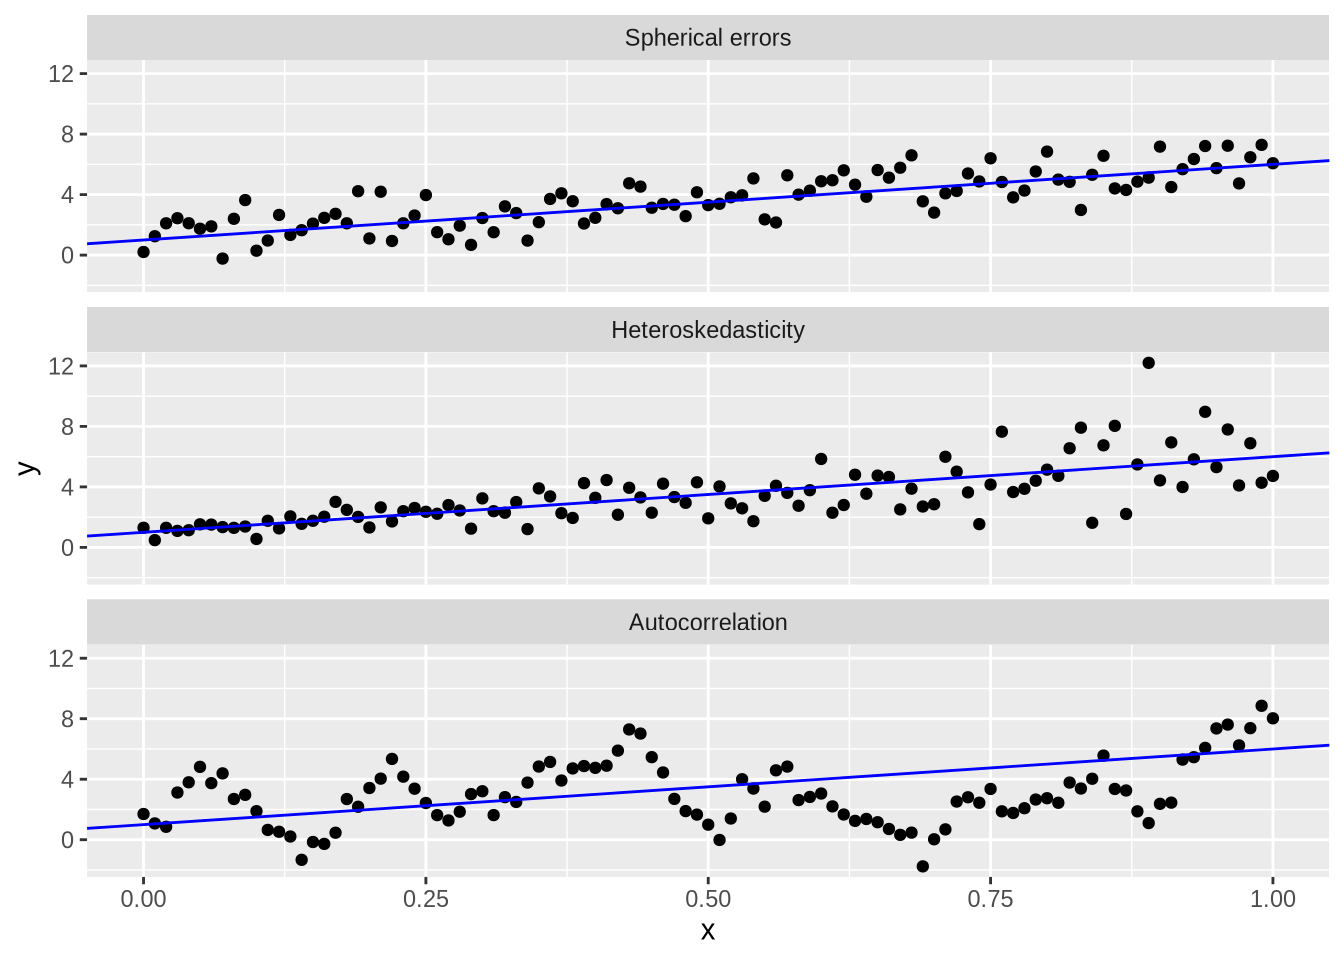
\includegraphics{pdaps_files/figure-latex/plot-spherical-errors-1.pdf}

Autocorrelation usually arises in time series analysis, which is beyond the scope of this course, so we will focus primarily on heteroskedasticity.

\hypertarget{generalized-least-squares}{%
\section{Generalized Least Squares}\label{generalized-least-squares}}

Suppose strict exogeneity holds, but spherical errors fails, with
\[
V[\epsilon \,|\, \mathbf{X}]
= \sigma^2 \Omega
= \sigma^2 \begin{bmatrix}
  \omega_{11} & \omega_{12} & \cdots & \omega_{1N} \\
  \omega_{12} & \omega_{22} & \cdots & \omega_{2N} \\
  \vdots & \vdots & \ddots & \vdots \\
  \omega_{1N} & \omega_{2N} & \cdots & \omega_{NN}
\end{bmatrix},
\]
where \(\Omega\) is known\footnote{Like any variance matrix, \(\Omega\) must be symmetric and positive definite. An \(N \times N\) matrix \(\mathbf{A}\) is positive definite if, for any \(N \times 1\) vector \(\mathbf{c} \neq \mathbf{0}\), the scalar \(\mathbf{c}^\top \mathbf{A} \mathbf{c} > 0\). Positive definiteness implies, among other things, that every diagonal entry of \(\Omega\) is positive and that \(\Omega\) is invertible.} and \(\sigma^2\) is unknown. In other words, we know the exact structure of heteroskedasticity and autocorrelation, up to a potentially unknown constant.

We derived the OLS estimator by finding the \(\hat{\beta}\) that minimizes the sum of squared errors,
\[
\text{SSE}
= \sum_n (Y_n - \mathbf{x}_n \cdot \hat{\beta})^2
= (\mathbf{Y} - \mathbf{X} \hat{\beta})^\top (\mathbf{Y} - \mathbf{X} \hat{\beta}).
\]
We derive its close cousin, the \emph{generalized least squares}, or GLS, estimator, by minimizing the \emph{weighted} sum of squared errors,
\[
\text{WSSE} = (\mathbf{Y} - \mathbf{X} \hat{\beta})^\top \Omega^{-1} (\mathbf{Y} - \mathbf{X} \hat{\beta}).
\]
I'll spare you the matrix calculus that follows, but suffice to say the resulting estimator is
\[
\hat{\beta}_{\text{GLS}} = (\mathbf{X}^\top \Omega^{-1} \mathbf{X})^{-1} \mathbf{X}^\top \Omega^{-1} \mathbf{Y}.
\]
It is easy to confirm that OLS is the special case of GLS with \(\Omega = \mathbf{I}\). Similar to the formula for OLS, the variance of GLS is
\[
V[\hat{\beta}_{\text{GLS}} \,|\, \mathbf{X}] = \sigma^2 (\mathbf{X}^\top \Omega^{-1} \mathbf{X})^{-1}.
\]

Like OLS, GLS is unbiased and consistent as long as we have strict exogeneity. Even if we get \(\Omega\) wrong---i.e., we misspecify the model of the error variance---GLS will still ``work'' in the sense of giving us an unbiased and consistent estimate of the coefficients. This is easy to confirm.
\[
\begin{aligned}
E [ \hat{\beta}_{\text{GLS}} \,|\, \mathbf{X} ]
&= E [ (\mathbf{X}^\top \Omega^{-1} \mathbf{X})^{-1} \mathbf{X}^\top \Omega^{-1} \mathbf{Y} \,|\, \mathbf{X} ] \\
&= (\mathbf{X}^\top \Omega^{-1} \mathbf{X})^{-1} \mathbf{X}^\top \Omega^{-1} E [\mathbf{Y} \,|\, \mathbf{X} ] \\
&= (\mathbf{X}^\top \Omega^{-1} \mathbf{X})^{-1} \mathbf{X}^\top \Omega^{-1} (\mathbf{X} \beta) \\
&= (\mathbf{X}^\top \Omega^{-1} \mathbf{X})^{-1} (\mathbf{X}^\top \Omega^{-1} \mathbf{X}) \beta \\
&= \beta.
\end{aligned}
\]
If we get \(\Omega\) right, then GLS has two important additional properties.

\begin{enumerate}
\def\labelenumi{\arabic{enumi}.}
\item
  Our estimate of the variance matrix,
  \[
  \hat{\Sigma} = \frac{\text{WSSE}}{N - K} (\mathbf{X}^\top \Omega^{-1} \mathbf{X})^{-1},
  \]
  is valid for inference using the same methods we discussed in the OLS case.
\item
  GLS is BLUE, per the Gauss-Markov theorem: there is no other unbiased linear estimator with lower standard errors.
\end{enumerate}

The first of these is pretty important; the second is just icing on the cake. The main problem with non-spherical errors is the threat they pose to inference from OLS. GLS fixes that---as long as we know \(\Omega\). More on this soon.

An important special case of GLS is when there is heteroskedasticity but no autocorrelation, so that
\[
\Omega = \sigma^2 \begin{bmatrix}
  \omega_{11} & 0 & \cdots & 0 \\
  0 & \omega_{22} & \cdots & 0 \\
  \vdots & \vdots & \ddots & \vdots \\
  0 & 0 & \cdots & \omega_{NN}
\end{bmatrix}.
\]
This special case is called \emph{weighted least squares}, since GLS gives us the same answer as if we ran OLS on the following ``weighted'' data:
\[
\mathbf{X}^* = \begin{bmatrix}
  x_{11} / \sqrt{\omega_{11}} & x_{12} / \sqrt{\omega_{11}} & \cdots & x_{1K} / \sqrt{\omega_{11}} \\
  x_{21} / \sqrt{\omega_{22}} & x_{22} / \sqrt{\omega_{22}} & \cdots & x_{2K} / \sqrt{\omega_{22}} \\
  \vdots & \vdots & \ddots & \vdots \\
  x_{N1} / \sqrt{\omega_{NN}} & x_{N2} / \sqrt{\omega_{NN}} & \cdots & x_{NK} / \sqrt{\omega_{NN}}
\end{bmatrix},
\mathbf{Y}^* = \begin{bmatrix}
  Y_1 / \sqrt{\omega_{11}} \\
  Y_2 / \sqrt{\omega_{22}} \\
  \vdots \\
  Y_N / \sqrt{\omega_{NN}}
\end{bmatrix}.
\]

\hypertarget{detecting-heteroskedasticity}{%
\section{Detecting Heteroskedasticity}\label{detecting-heteroskedasticity}}

If you don't have prior knowledge of the variance structure of the error term, you may be interested in testing whether the homoskedasticity assumption of OLS is viable. In a bivariate regression model, you can usually detect heteroskedasticity via the eye test. Not so much when you have multiple covariates. In this case, you may want to formally test for heteroskedasticity.

There are a few such tests, but we will just talk about the \emph{Breusch-Pagan test}, which was developed by \citet{breusch1980lagrange} and refined by \citet{koenker1982robust}. The null hypothesis of the test is that \(V[\epsilon_i \,|\, \mathbf{X}] = \sigma^2\) for all \(i = 1, \ldots, N\). The test procedure is as follows.

\begin{enumerate}
\def\labelenumi{\arabic{enumi}.}
\tightlist
\item
  Calculate the OLS estimate, \(\hat{\beta}_{\text{OLS}}\).
\item
  Calculate the OLS residuals, \(\hat{e} = Y - \mathbf{X} \hat{\beta}_{\text{OLS}}\). Let \(\hat{u}\) be the vector of squared residuals, \(\hat{u} = (\hat{e}_1^2, \ldots, \hat{e}_N^2)\).
\item
  Run a regression of \(\hat{u}\) on \(\mathbf{Z}\), an \(N \times q\) matrix of covariates. Let \(R_{\hat{u}}^2\) denote the \(R^2\) of this regression.
\item
  Reject the null hypothesis if \(N R_{\hat{u}}^2\) exceeds the critical value for a \(\chi_{q - 1}^2\) distribution.
\end{enumerate}

In the canonical version of this test, \(\mathbf{Z}\) is equal to \(\mathbf{X}\). A more powerful version is the \emph{White test} \citep{white1980heteroskedasticity}, in which \(\mathbf{Z}\) contains each variable in \(\mathbf{X}\) as well as all second-order terms (squares and interactions).

\hypertarget{heteroskedasticity-of-unknown-form}{%
\section{Heteroskedasticity of Unknown Form}\label{heteroskedasticity-of-unknown-form}}

Suppose we know there is heteroskedasticity but we don't trust ourselves to properly specify the error variances to run weighted least squares.\footnote{There is an in-between solution known as \emph{feasible generalized least squares}, whereby we estimate \(\Omega\) from the data. This requires placing some structure on \(\Omega\), and the resulting estimator will be consistent but not unbiased.} Then we do not have an efficient estimator of \(\beta\). We might be all right with that, but we would really like to have a good estimator for the standard errors of the OLS estimator, so that we can test hypotheses about the coefficients. Happily, we can estimate the variance matrix of the OLS estimator consistently even in the presence of heteroskedasticity.

\emph{White's heteroskedasticity-consistent estimator} \citep{white1980heteroskedasticity} of the variance matrix starts by forming a diagonal matrix out of the squared residuals,
\[
\hat{\mathbf{U}}
=
\begin{bmatrix}
\hat{u}_1 & 0 & \cdots & 0 \\
0 & \hat{u}_2 & \cdots & 0 \\
\vdots & \vdots & \ddots & \vdots \\
0 & 0 & \cdots & \hat{u}_N
\end{bmatrix}
=
\begin{bmatrix}
\hat{e}_1^2 & 0 & \cdots & 0 \\
0 & \hat{e}_2^2 & \cdots & 0 \\
\vdots & \vdots & \ddots & \vdots \\
0 & 0 & \cdots & \hat{e}_N^2
\end{bmatrix}
\]
This lets us form the ``meat'' of the ``sandwich'' that is White's estimator of the OLS variance matrix:
\[
\hat{\Sigma}_{\text{HC}}
=
(\mathbf{X}^\top \mathbf{X})^{-1} \mathbf{X}^\top \hat{\mathbf{U}} \mathbf{X} (\mathbf{X}^\top \mathbf{X})^{-1}.
\]
You know I love proofs, but I am not even going to attempt to prove that this consistently estimates the (asymptotic) variance matrix of \(\hat{\beta}_{\text{OLS}}\). See \citet[pp.~198--199]{greene} for a sketch of the proof.

White's estimator is consistent but not unbiased, so we may want to apply a sort of bias correction in small samples. A popular choice is the so-called ``HC1'' estimator, which corrects for the number of parameters estimated the same way the usual OLS variance estimator does:
\[
\hat{\Sigma}_{\text{HC1}} = \frac{N}{N - K} \hat{\Sigma}_{\text{HC}}
\]
In this scheme, the standard White estimator is called the ``HC'' or ``HC0'' estimator. There are many other consistent estimators that apply some or other finite-sample correction; see \citet{mackinnon1985some} for the gory details.

Because of its association with the \texttt{,\ robust} option in Stata, people sometimes call the White estimator of the standard errors ``robust standard errors''. Don't do that. In your own work, if you estimate and report heteroskedasticity-consistent standard errors, report that you use the \citet{white1980heteroskedasticity} estimator of the standard errors, and specify which variant (HC0, HC1, and so on). Remember that your goal is to give others enough information to replicate your analysis even if they don't have your code---``robust standard errors'' has too many interpretations to accomplish that.

Finally, it is important to know that weighted least squares and heteroskedasticity-consistent standard errors are not mutually exclusive approaches. If you have a suspicion about the error variances that you think can improve the precision of the regression, but you are not totally comfortable with committing to WLS for inference, you can calculate heteroskedasticity-consistent standard errors for a WLS (or GLS) fit.

\hypertarget{appendix-implementation-in-r}{%
\section{Appendix: Implementation in R}\label{appendix-implementation-in-r}}

We'll be using the following packages:

\begin{Shaded}
\begin{Highlighting}[]
\KeywordTok{library}\NormalTok{(}\StringTok{"tidyverse"}\NormalTok{)}
\KeywordTok{library}\NormalTok{(}\StringTok{"broom"}\NormalTok{)}
\KeywordTok{library}\NormalTok{(}\StringTok{"car"}\NormalTok{)}
\KeywordTok{library}\NormalTok{(}\StringTok{"lmtest"}\NormalTok{)}
\KeywordTok{library}\NormalTok{(}\StringTok{"sandwich"}\NormalTok{)}
\end{Highlighting}
\end{Shaded}

We will use data from the \textbf{car} package on professors' salaries. This is a topic that, ideally, will be of great concern to you in 5ish years.

\begin{Shaded}
\begin{Highlighting}[]
\KeywordTok{data}\NormalTok{(Salaries)}
\KeywordTok{head}\NormalTok{(Salaries)}
\end{Highlighting}
\end{Shaded}

\begin{verbatim}
##        rank discipline yrs.since.phd yrs.service  sex salary
## 1      Prof          B            19          18 Male 139750
## 2      Prof          B            20          16 Male 173200
## 3  AsstProf          B             4           3 Male  79750
## 4      Prof          B            45          39 Male 115000
## 5      Prof          B            40          41 Male 141500
## 6 AssocProf          B             6           6 Male  97000
\end{verbatim}

\hypertarget{generalized-least-squares-1}{%
\subsection{Generalized Least Squares}\label{generalized-least-squares-1}}

Let us model a professor's salary as a function of the number of years since she received her PhD. If we glance at the data, we see obvious heteroskedasticity.

\begin{Shaded}
\begin{Highlighting}[]
\KeywordTok{ggplot}\NormalTok{(Salaries, }\KeywordTok{aes}\NormalTok{(}\DataTypeTok{x =}\NormalTok{ yrs.since.phd, }\DataTypeTok{y =}\NormalTok{ salary)) }\OperatorTok{+}
\StringTok{    }\KeywordTok{geom\_point}\NormalTok{()}
\end{Highlighting}
\end{Shaded}

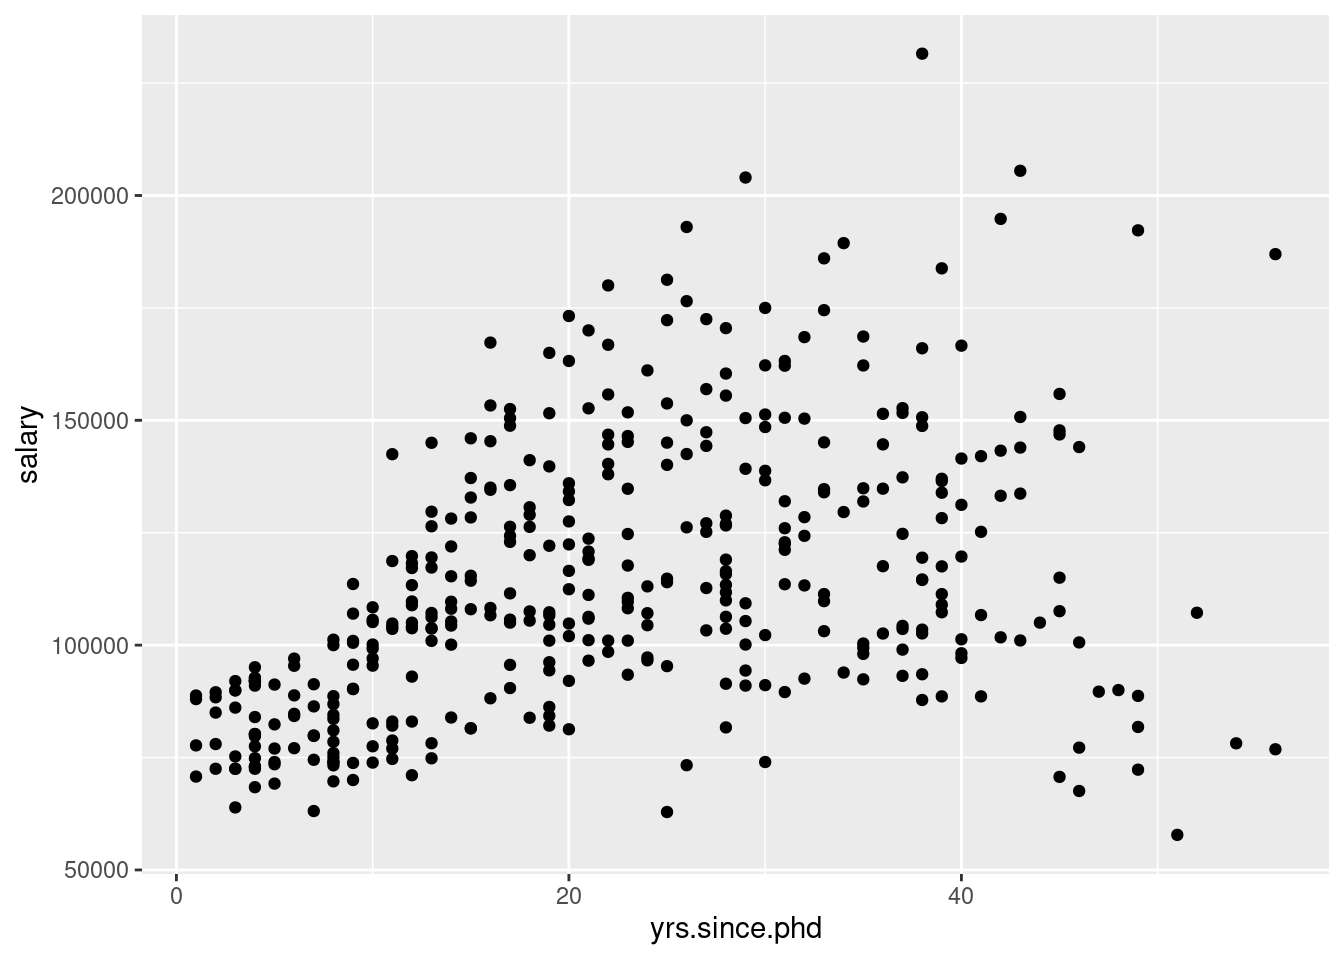
\includegraphics{pdaps_files/figure-latex/salaries-plot-hetero-1.pdf}

There is much more variation in the salaries of professors 30+ years into their careers than in those who are fresh out of grad school. If we want the most precise model of the relationship between years since PhD and salary, we might want to place more weight on early-career professors and less on late-career professors.

Remember that weighted least squares is the special case of GLS where the off-diagonal elements of \(\Omega\) are zero (i.e., there is heteroskedasticity but no autocorrelation):
\[
\Omega = \sigma^2 \begin{bmatrix}
  \omega_{11} & 0 & \cdots & 0 \\
  0 & \omega_{22} & \cdots & 0 \\
  \vdots & \vdots & \ddots & \vdots \\
  0 & 0 & \cdots & \omega_{NN}
\end{bmatrix}.
\]
To run weighted least squares in R, we just use the \texttt{weights} argument to the \texttt{lm()} function. As an example, let's set
\[
\omega_{nn} = \frac{1}{\text{Years Since PhD}_n}
\]
for each observation \(n\), to place the greatest weight on early-career observations. We will first run a baseline OLS model, then compare to the weighted model.

\begin{Shaded}
\begin{Highlighting}[]
\NormalTok{ols\_salaries \textless{}{-}}\StringTok{ }\KeywordTok{lm}\NormalTok{(salary }\OperatorTok{\textasciitilde{}}\StringTok{ }\NormalTok{yrs.since.phd }\OperatorTok{+}\StringTok{ }\NormalTok{yrs.service,}
                   \DataTypeTok{data =}\NormalTok{ Salaries)}
\KeywordTok{summary}\NormalTok{(ols\_salaries)}
\end{Highlighting}
\end{Shaded}

\begin{verbatim}
## 
## Call:
## lm(formula = salary ~ yrs.since.phd + yrs.service, data = Salaries)
## 
## Residuals:
##    Min     1Q Median     3Q    Max 
## -79735 -19823  -2617  15149 106149 
## 
## Coefficients:
##               Estimate Std. Error t value Pr(>|t|)    
## (Intercept)    89912.2     2843.6  31.620  < 2e-16 ***
## yrs.since.phd   1562.9      256.8   6.086 2.75e-09 ***
## yrs.service     -629.1      254.5  -2.472   0.0138 *  
## ---
## Signif. codes:  0 '***' 0.001 '**' 0.01 '*' 0.05 '.' 0.1 ' ' 1
## 
## Residual standard error: 27360 on 394 degrees of freedom
## Multiple R-squared:  0.1883, Adjusted R-squared:  0.1842 
## F-statistic: 45.71 on 2 and 394 DF,  p-value: < 2.2e-16
\end{verbatim}

\begin{Shaded}
\begin{Highlighting}[]
\NormalTok{wls\_salaries \textless{}{-}}\StringTok{ }\KeywordTok{lm}\NormalTok{(salary }\OperatorTok{\textasciitilde{}}\StringTok{ }\NormalTok{yrs.since.phd }\OperatorTok{+}\StringTok{ }\NormalTok{yrs.service,}
                   \DataTypeTok{weights =} \DecValTok{1} \OperatorTok{/}\StringTok{ }\NormalTok{yrs.since.phd,}
                   \DataTypeTok{data =}\NormalTok{ Salaries)}
\KeywordTok{summary}\NormalTok{(wls\_salaries)}
\end{Highlighting}
\end{Shaded}

\begin{verbatim}
## 
## Call:
## lm(formula = salary ~ yrs.since.phd + yrs.service, data = Salaries, 
##     weights = 1/yrs.since.phd)
## 
## Weighted Residuals:
##      Min       1Q   Median       3Q      Max 
## -13520.2  -4386.2    -91.3   4101.0  16045.7 
## 
## Coefficients:
##               Estimate Std. Error t value Pr(>|t|)    
## (Intercept)    79671.5     1460.3  54.560  < 2e-16 ***
## yrs.since.phd   1753.3      242.0   7.246 2.27e-12 ***
## yrs.service     -288.9      264.6  -1.092    0.276    
## ---
## Signif. codes:  0 '***' 0.001 '**' 0.01 '*' 0.05 '.' 0.1 ' ' 1
## 
## Residual standard error: 5759 on 394 degrees of freedom
## Multiple R-squared:  0.4274, Adjusted R-squared:  0.4245 
## F-statistic: 147.1 on 2 and 394 DF,  p-value: < 2.2e-16
\end{verbatim}

Compared to OLS, our WLS model yields a stronger relationship between years since the PhD and the expected value of a professor's salary. In addition, we estimate a smaller coefficient on years of service, and would no longer reject the null hypothesis of no relationship there.

Which model is better, OLS or WLS? It depends on whether our weights correspond to the true relative variance in the error term. In this case, we've specified a pretty aggressive weighting scheme---a professor with 1 year of service gets double the weight of a professor with 2 years of service. An alternative weighting scheme would give us different results. The ``best'' model is the one that best corresponds to the true \(\Omega\), which unfortunately is hard to know in advance. The best we can do is apply theory and judgment in a thoughtful way.

In the (relatively unlikely) event that you are pre-specifying \(\Omega\) with autocorrelations, you can use the \texttt{lm.gls()} function from the \textbf{MASS} package. The \texttt{gls()} function from the \textbf{nlme} package performs \emph{feasible} generalized least squares, whereby we write \(\Omega\) as a function of a few parameters, estimate those parameters, and run the subsequent GLS model.

\hypertarget{breusch-pagan-test}{%
\subsection{Breusch-Pagan Test}\label{breusch-pagan-test}}

We already used the ``eye test'' to confirm the presence of heteroskedasticity in the relationship we are modeling, but let's see how we would use the Breusch-Pagan test to confirm our suspicion. For this we use the \texttt{bptest()} function from the \textbf{lmtest} package.

\begin{Shaded}
\begin{Highlighting}[]
\KeywordTok{bptest}\NormalTok{(ols\_salaries)}
\end{Highlighting}
\end{Shaded}

\begin{verbatim}
## 
##  studentized Breusch-Pagan test
## 
## data:  ols_salaries
## BP = 49.864, df = 2, p-value = 1.486e-11
\end{verbatim}

By default, \texttt{bptest()} uses the same variables as in the original regression in the regression of the squared residuals. To perform the White test, we can use an extra argument to \texttt{bptest()} to specify a different model formula.

\begin{Shaded}
\begin{Highlighting}[]
\KeywordTok{bptest}\NormalTok{(ols\_salaries,}
       \OperatorTok{\textasciitilde{}}\StringTok{ }\NormalTok{yrs.since.phd }\OperatorTok{*}\StringTok{ }\NormalTok{yrs.service }\OperatorTok{+}\StringTok{ }\KeywordTok{I}\NormalTok{(yrs.since.phd}\OperatorTok{\^{}}\DecValTok{2}\NormalTok{) }\OperatorTok{+}\StringTok{ }\KeywordTok{I}\NormalTok{(yrs.service}\OperatorTok{\^{}}\DecValTok{2}\NormalTok{),}
       \DataTypeTok{data =}\NormalTok{ Salaries)}
\end{Highlighting}
\end{Shaded}

\begin{verbatim}
## 
##  studentized Breusch-Pagan test
## 
## data:  ols_salaries
## BP = 60.486, df = 5, p-value = 9.644e-12
\end{verbatim}

In this case, regardless of which test we use, we reject the null hypothesis of homoskedasticity.

\hypertarget{heteroskedasticity-consistent-standard-errors}{%
\subsection{Heteroskedasticity-Consistent Standard Errors}\label{heteroskedasticity-consistent-standard-errors}}

To calculate the White estimator and its friends in R, we use the \texttt{vcovHC()} function from the \textbf{sandwich} package.

\begin{Shaded}
\begin{Highlighting}[]
\NormalTok{vcv0 \textless{}{-}}\StringTok{ }\KeywordTok{vcovHC}\NormalTok{(ols\_salaries, }\DataTypeTok{type =} \StringTok{"HC0"}\NormalTok{)}
\NormalTok{vcv0}
\end{Highlighting}
\end{Shaded}

\begin{verbatim}
##               (Intercept) yrs.since.phd yrs.service
## (Intercept)     5809136.7    -340724.37   111807.54
## yrs.since.phd   -340724.4      77168.04   -75508.41
## yrs.service      111807.5     -75508.41    91090.58
\end{verbatim}

To use HC1 (or another one of the finite-sample corrections to the ordinary White estimate), change the \texttt{type} argument to, e.g., \texttt{type\ =\ "HC1"}. See \texttt{?vcovHC} for all the options.

To create a ``regression table'' using our new ``robust'' standard errors, we can use the \texttt{coeftest()} function from the \textbf{lmtest} package.

\begin{Shaded}
\begin{Highlighting}[]
\KeywordTok{coeftest}\NormalTok{(ols\_salaries)  }\CommentTok{\# Original table}
\end{Highlighting}
\end{Shaded}

\begin{verbatim}
## 
## t test of coefficients:
## 
##               Estimate Std. Error t value  Pr(>|t|)    
## (Intercept)   89912.18    2843.56 31.6196 < 2.2e-16 ***
## yrs.since.phd  1562.89     256.82  6.0856 2.754e-09 ***
## yrs.service    -629.10     254.47 -2.4722   0.01385 *  
## ---
## Signif. codes:  0 '***' 0.001 '**' 0.01 '*' 0.05 '.' 0.1 ' ' 1
\end{verbatim}

\begin{Shaded}
\begin{Highlighting}[]
\KeywordTok{coeftest}\NormalTok{(ols\_salaries, }\DataTypeTok{vcov =}\NormalTok{ vcv0)  }\CommentTok{\# With corrected SEs}
\end{Highlighting}
\end{Shaded}

\begin{verbatim}
## 
## t test of coefficients:
## 
##               Estimate Std. Error t value  Pr(>|t|)    
## (Intercept)   89912.18    2410.22 37.3046 < 2.2e-16 ***
## yrs.since.phd  1562.89     277.79  5.6261 3.501e-08 ***
## yrs.service    -629.10     301.81 -2.0844   0.03777 *  
## ---
## Signif. codes:  0 '***' 0.001 '**' 0.01 '*' 0.05 '.' 0.1 ' ' 1
\end{verbatim}

Just like ordinary regression tables, the ones made by \texttt{coeftest()} can be ``swept'' into data frames using the tools in \textbf{broom}:

\begin{Shaded}
\begin{Highlighting}[]
\KeywordTok{tidy}\NormalTok{(}\KeywordTok{coeftest}\NormalTok{(ols\_salaries, }\DataTypeTok{vcov =}\NormalTok{ vcv0))}
\end{Highlighting}
\end{Shaded}

\begin{verbatim}
## # A tibble: 3 x 5
##   term          estimate std.error statistic   p.value
##   <chr>            <dbl>     <dbl>     <dbl>     <dbl>
## 1 (Intercept)     89912.     2410.     37.3  2.33e-131
## 2 yrs.since.phd    1563.      278.      5.63 3.50e-  8
## 3 yrs.service      -629.      302.     -2.08 3.78e-  2
\end{verbatim}

You may also want to use the White-estimated standard errors to conduct Wald tests of linear hypotheses. You can do that by supplying the relevant estimated variance matrix to the \texttt{vcov} argument of \texttt{linearHypothesis()}:

\begin{Shaded}
\begin{Highlighting}[]
\KeywordTok{linearHypothesis}\NormalTok{(ols\_salaries,}
                 \KeywordTok{c}\NormalTok{(}\StringTok{"yrs.since.phd = 1500"}\NormalTok{, }\StringTok{"yrs.service = {-}500"}\NormalTok{),}
                 \DataTypeTok{vcov =}\NormalTok{ vcv0,}
                 \DataTypeTok{test =} \StringTok{"Chisq"}\NormalTok{)}
\end{Highlighting}
\end{Shaded}

\begin{verbatim}
## Linear hypothesis test
## 
## Hypothesis:
## yrs.since.phd = 1500
## yrs.service = - 500
## 
## Model 1: restricted model
## Model 2: salary ~ yrs.since.phd + yrs.service
## 
## Note: Coefficient covariance matrix supplied.
## 
##   Res.Df Df  Chisq Pr(>Chisq)
## 1    396                     
## 2    394  2 0.3166     0.8536
\end{verbatim}

Finally, remember how earlier we talked about how the WLS estimates are only as good as the weights you choose. If they're not the true weights, then WLS is not efficient and the standard error estimator is inconsistent. We can't fix the first problem, but we can fix the second. To wit, you can estimate heteroskedasticity-consistent standard errors for WLS models too.

\begin{Shaded}
\begin{Highlighting}[]
\NormalTok{vcv0\_wls \textless{}{-}}\StringTok{ }\KeywordTok{vcovHC}\NormalTok{(wls\_salaries, }\DataTypeTok{type =} \StringTok{"HC0"}\NormalTok{)}
\KeywordTok{coeftest}\NormalTok{(wls\_salaries)  }\CommentTok{\# Original}
\end{Highlighting}
\end{Shaded}

\begin{verbatim}
## 
## t test of coefficients:
## 
##               Estimate Std. Error t value  Pr(>|t|)    
## (Intercept)   79671.54    1460.26 54.5599 < 2.2e-16 ***
## yrs.since.phd  1753.29     241.95  7.2465 2.273e-12 ***
## yrs.service    -288.93     264.64 -1.0918    0.2756    
## ---
## Signif. codes:  0 '***' 0.001 '**' 0.01 '*' 0.05 '.' 0.1 ' ' 1
\end{verbatim}

\begin{Shaded}
\begin{Highlighting}[]
\KeywordTok{coeftest}\NormalTok{(wls\_salaries, }\DataTypeTok{vcov =}\NormalTok{ vcv0\_wls)  }\CommentTok{\# Corrected}
\end{Highlighting}
\end{Shaded}

\begin{verbatim}
## 
## t test of coefficients:
## 
##               Estimate Std. Error t value  Pr(>|t|)    
## (Intercept)   79671.54    1473.72 54.0616 < 2.2e-16 ***
## yrs.since.phd  1753.29     244.71  7.1647 3.862e-12 ***
## yrs.service    -288.93     271.59 -1.0639     0.288    
## ---
## Signif. codes:  0 '***' 0.001 '**' 0.01 '*' 0.05 '.' 0.1 ' ' 1
\end{verbatim}

So if you have a good idea about the residual variances but aren't sure you've nailed it down, you can have the best of both worlds---at least in terms of large-sample hypothesis testing.

\hypertarget{crisis}{%
\chapter{The Statistical Crisis in Science}\label{crisis}}

As a general rule, I do not believe the statistical results reported in political science publications. More to the point, absent compelling evidence to the contrary, I assume that:

\begin{itemize}
\item
  Reported effect sizes are biased upward in magnitude. The marginal effect of the key variable(s) in the population is likely less dramatic than what is reported.
\item
  Reported \(p\)-values are biased downward. The probability of making a Type I error, in case the null hypothesis were false and one followed the \emph{actual} procedure that led to the reported results, is greater than what is reported.
\end{itemize}

My position is not one of blind skepticism. It follows, perhaps ironically, from empirical research showing that far more than 5 percent of studies do not replicate upon re-testing \citep{open2015estimating}. \citet{ioannidis2005most} puts it bluntly: ``Most published research findings are false.'' Today we'll discuss why.

I'll follow \citet{young2008current}'s economic analogy. Consider scientific publication as an economic activity, where researchers ``sell'' findings to journals in exchange for prestige.\footnote{Have you ever wondered why academic journal subscriptions cost unholy amounts of money, yet the authors, reviewers, and (usually) editors are unpaid?} The \emph{demand-side problem} is that journals will only ``buy'' statistically significant findings. Even absent any effects on author behavior, this practice makes published findings a biased sample of actual findings. But of course there are effects on author behavior. The \emph{supply-side problem} is that authors try to produce ``statistically significant'' findings instead of scientifically sound findings.

There is far more out there on the replication crisis in science than we can cover in a week. Sanjay Srivastava's faux syllabus, \href{https://hardsci.wordpress.com/2016/08/11/everything-is-fucked-the-syllabus/}{``Everything is fucked''}, provides a more comprehensive treatment.

\hypertarget{publication-bias}{%
\section{Publication Bias}\label{publication-bias}}

If you open up an issue of any empirically oriented political science journal, you will not read many abstracts that conclude ``We were unable to reject the null hypothesis of no effect.'' You probably won't see any. The prevailing attitude of reviewers and editors is that only significant results are interesting and only interesting results are worth publishing---so only significant results get published.

Consequently, published empirical findings are not a representative sample of all empirical findings. \href{http://andrewgelman.com/2011/09/10/the-statistical-significance-filter/}{Andrew Gelman calls this the \emph{statistical significance filter}}: the publication process only reveals the findings of some studies, namely those that achieve statistical significance. If you draw your beliefs from scientific journals (particularly prestigious ones, as \citet{ioannidis2008most} notes), you will end up with some false ideas about how the world works.

Some of these beliefs will be Type I errors: you will reject null hypotheses that are true. Suppose there is a treatment \(T\) that has no effect on an outcome \(Y\), and 100 labs run separate experiments of the effect of \(T\) on \(Y\). We would expect about 95 of these experiments to (correctly) fail to reject the null hypotheses, and about 5 to (incorrectly) reject it. But if some of the significant findings get published and none of the insignificant ones do, you will end up incorrectly believing the treatment affects the outcome.

But the statistical significance filter has another, less obvious---and thus more pernicious---effect on our inferences. Assume that the null hypothesis is indeed false: that the treatment \(T\) has an effect on the outcome \(Y\). Suppose once again that 100 labs run separate experiments of the effect of \(T\) on \(Y\). Depending on the power of the experiments, some proportion of them will (incorrectly) fail to reject the null hypothesis, and the remainder will (correctly) reject it. Because of the statistical significance filter, only the ones that reject the null hypothesis will get published.

That's not so bad, right? Only the studies that reject the null hypothesis get published, but the null hypothesis is wrong! The problem comes in when we want to evaluate the size of the effect---what political scientists like to call ``substantive significance.''\footnote{Mini rant: In my admittedly short career in political science, I have seen zero talks or papers claim to have found a statistically significant but substantively insignificant result. I have, however, seen talks that claimed a 0.001\% increase constituted a substantively significant finding. Without a threshold for substantive significance that is decided on \emph{before} the results are obtained, any claim about substantive significance is incredible.} On average, the statistically significant studies will tend to overestimate the magnitude of the effect. Viewing studies through the statistical significance filter, we will correctly infer that there is an effect, but we will systematically overestimate how strong it is.

Why does the statistical significance filter result in an overestimate of effect magnitudes? Imagine that the population regression coefficient is real but small, say \(\beta_k = 0.1\). Then the sampling distribution of \(\hat{\beta}_k\) will look something like the following graph.

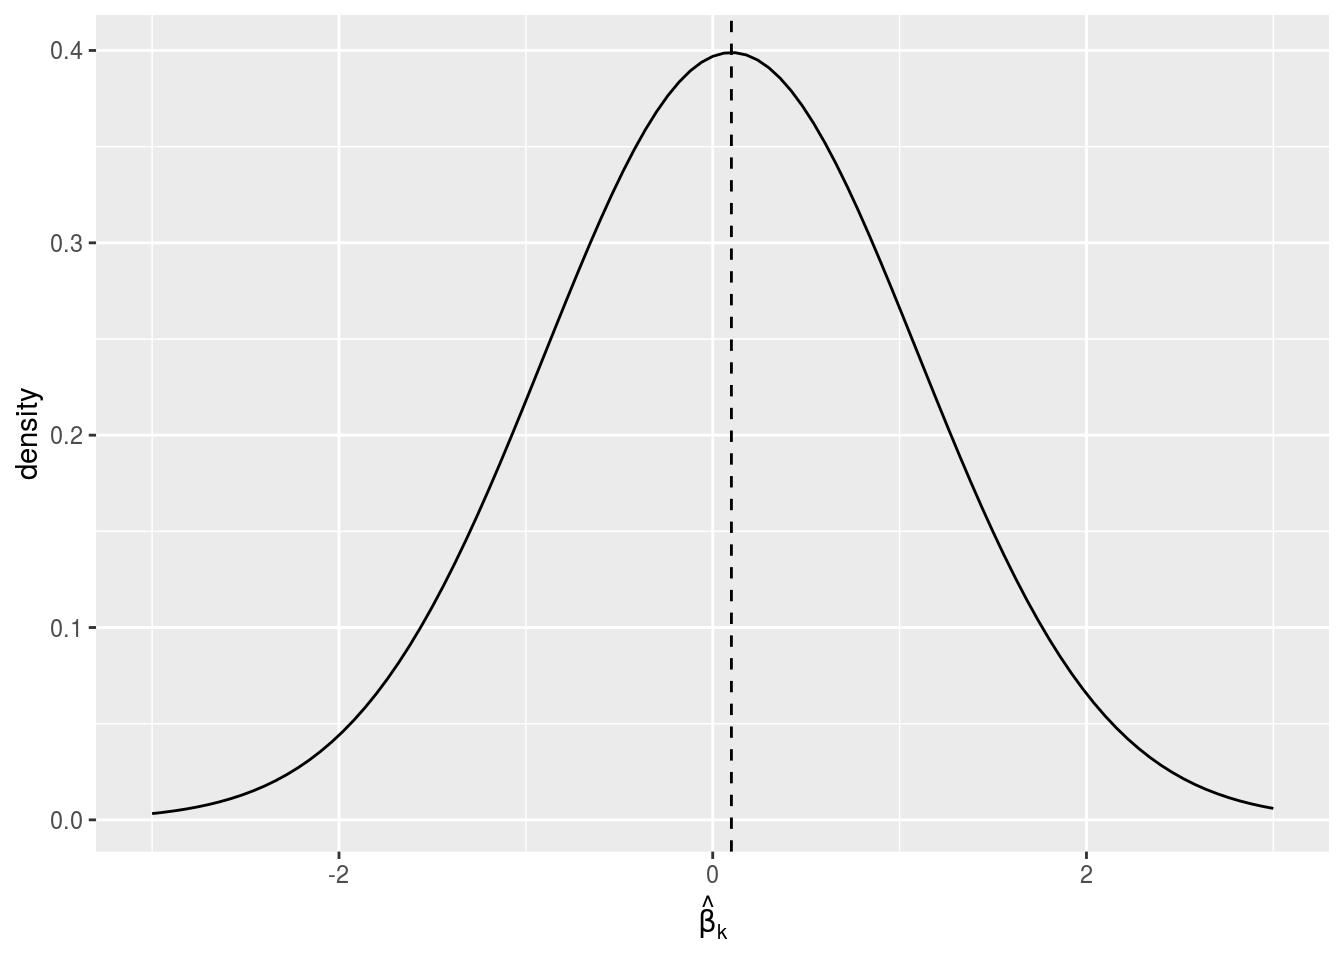
\includegraphics{pdaps_files/figure-latex/filter-plot-1.pdf}

Since the population parameter is close to zero, we are rather likely to yield a sample estimate close to zero. With a small sample size, sample estimates close to zero are likely to be statistically insignificant. Under the statistical significance filter, only the results in the ``tails'' of the distribution will end up being published.

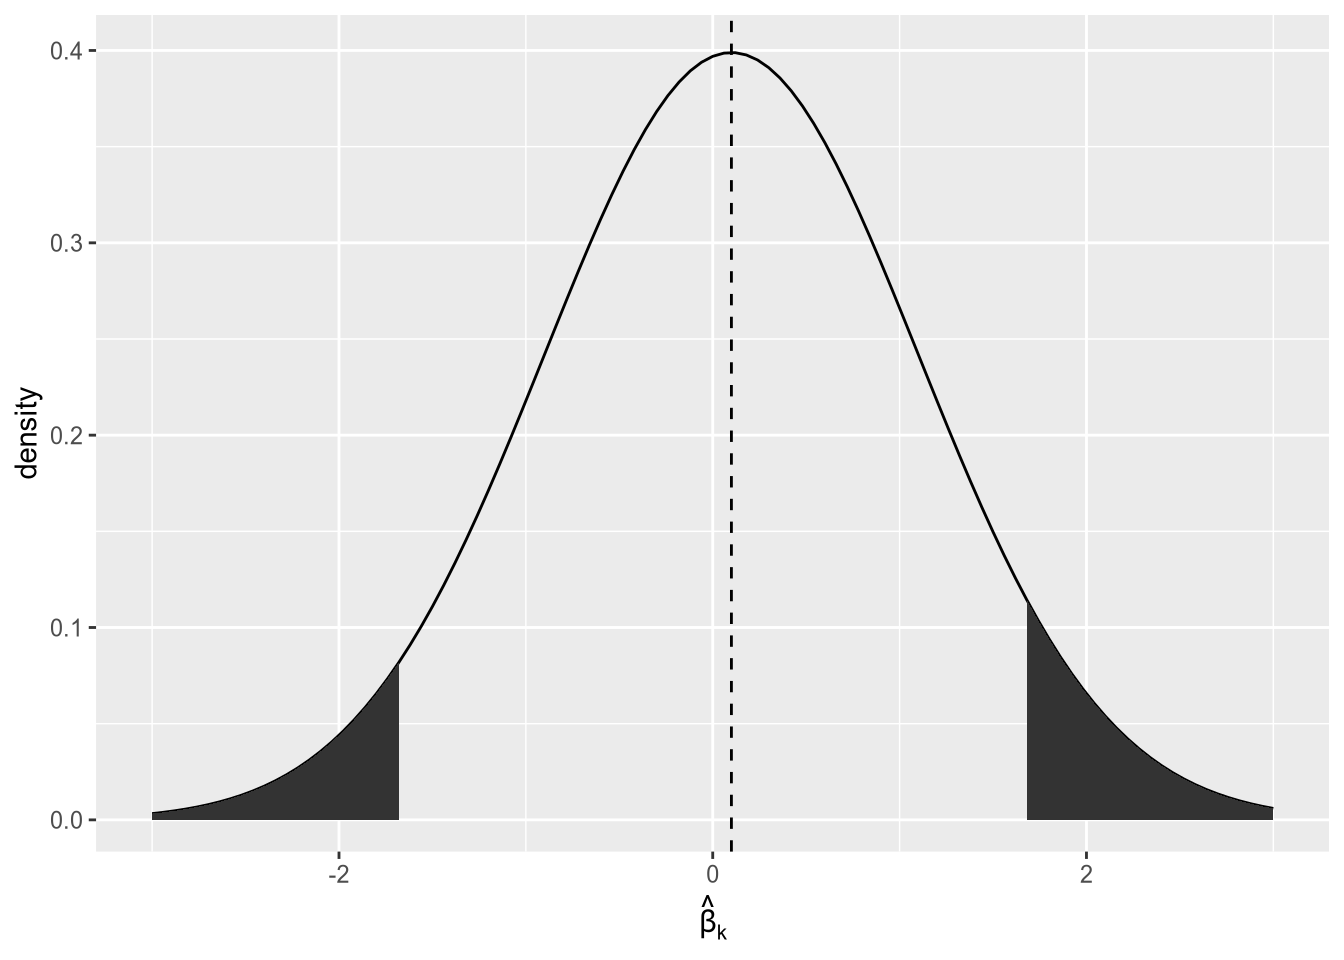
\includegraphics{pdaps_files/figure-latex/filter-plot-2-1.pdf}

The first time I read about this result, on Andrew Gelman's blog, I didn't believe it. (I \emph{should} have believed it, because he's a professional statistician and I'm not.) So I fired up R and ran a simulation to answer: if we only report our estimate of \(\beta_k\) when it's statistically significant, will we overestimate its magnitude on average? In your R session this week, you will run a version of this same simulation.

\hypertarget{p-hacking}{%
\section{\texorpdfstring{\(p\)-Hacking}{p-Hacking}}\label{p-hacking}}

The statistical significance filter is a demand-side problem. The demand (by journals) for ``insignificant'' findings is too low. This in turn creates supply-side problems. Scientists' careers depend on their ability to publish their findings. Since there is no demand for insignificant findings, scientists do what they can to conjure up significant results. In the best case scenario, this means devoting effort to projects with a high prior probability of turning up significant, rather than riskier endeavors. In the worst case, it means engaging in vaguely-to-definitely unethical statistical practices in a desperate search for significance.

One way to \(p\)-hack is to just define the significance level \emph{post hoc}.

\begin{figure}
\centering
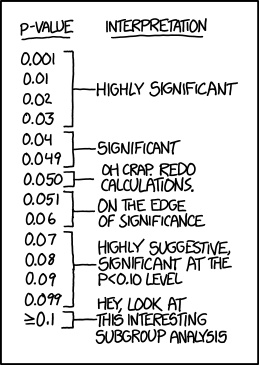
\includegraphics{p_values.png}
\caption{\href{https://xkcd.com/1478/}{XKCD \#1478.}}
\end{figure}

Luckily, this is pretty transparent. The convention, for better or worse, is a significance level of 0.05, and it's easy to notice deviations from the convention. Look for the ``daggers'' in people's regression tables, or language like ``comes close to statistical significance''. Matthew Hankins' blog post \href{https://mchankins.wordpress.com/2013/04/21/still-not-significant-2/}{``Still Not Significant''} is a comprehensive compendium of the weasel language people use to try to dress up their insignificant findings. See also \citet{pritschet2016marginally}.

The more pernicious form of \(p\)-hacking is going fishing for something significant after one's original hypothesis test ``fails.'' Let us once again imagine a lab performing an experiment. They are interested in the effect of a treatment \(T\) on an outcome \(Y\). To make it concrete, suppose the treatment is reading a particular editorial, and the outcome is where the respondent places himself or herself on a left-right ideological scale ranging between 0 and 1. The lab spends a lot of time and money recruiting subjects, running the experiment, and tabulating the data. They get their spreadsheet together, load their data into R, test for a treatment effect \ldots{} and fail to reject the null hypothesis.

Damn. All that effort wasted, for a result that can't be published. But wait! The op-ed was written by a man, and his picture appeared next to it. It seems plausible that it might only have an effect on men, or only one on women. So just to see, the lab re-runs the test once just for men and once just for women. They get a \(p\)-value just below \(0.05\) for the male subsample! Hooray! This is at least potentially a publishable finding!

What's wrong with this picture? Let's go back to the formal definition of the significance level.

\begin{quote}
The significance level of a hypothesis test is the probability of rejecting the null hypothesis when the null hypothesis is true.
\end{quote}

If the null hypothesis is true, and 100 labs run the same experiment on it, we should expect about 5 of them to end up incorrectly rejecting the null hypothesis. Similarly, go back to the formal definition of a \(p\)-value.

\begin{quote}
The \(p\)-value of a test statistic is the probability of yielding a test statistic at least as extreme when the null hypothesis is true.
\end{quote}

If the null hypothesis is true, we should expect only about 10 out of 100 labs to end up with \(p \leq 0.10\), 5 out of 100 to have \(p \leq 0.05\), and so on.

The problem with this hypothetical procedure---testing \emph{post hoc} for effects within subgroups after the main test comes back insignificant---is that the stated significance level is not the real significance level. If you run three different tests and reject the null hypothesis if \emph{any} of them comes back with \(p \leq 0.05\), you will reject the null hypothesis more often than 5\% of the time. In our running hypothetical example, the lab's reported \(p\)-value of 0.05 is a lie.

\begin{figure}
\centering
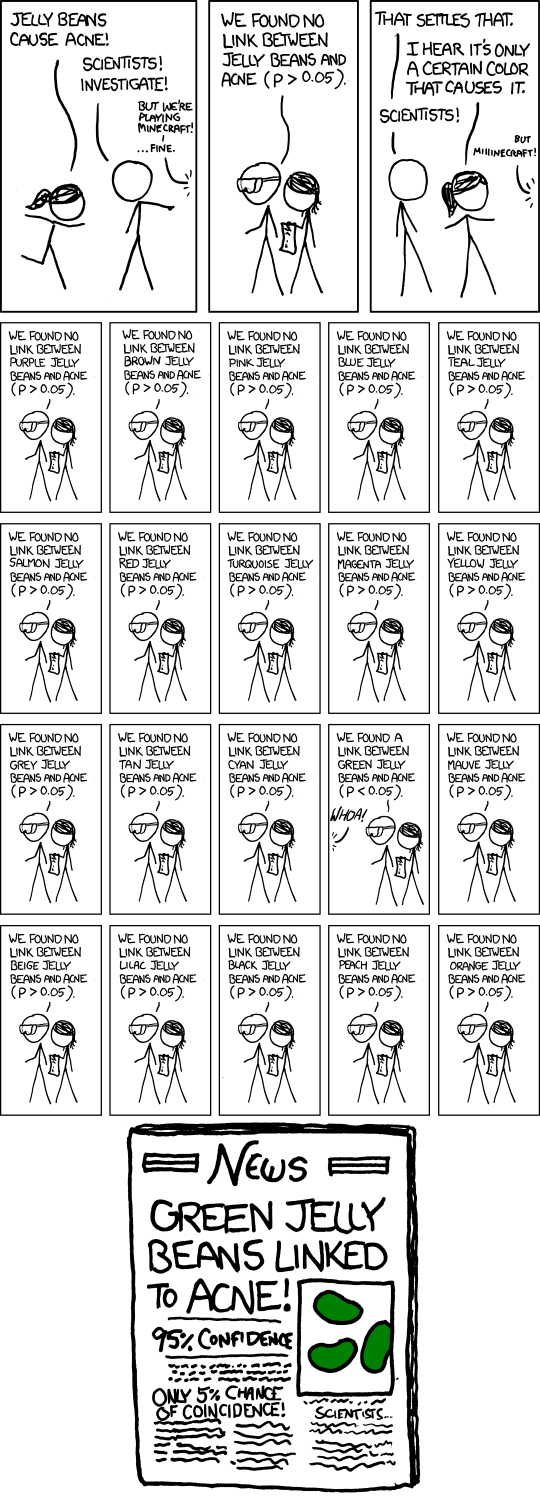
\includegraphics{significant.png}
\caption{\href{https://xkcd.com/882/}{XKCD \#882.}}
\end{figure}

There are many ways to \(p\)-hack:

\begin{itemize}
\tightlist
\item
  Splitting up data by subgroups \emph{post hoc}
\item
  Changing the set of variables you control for
\item
  Changing the operationalization of the covariate of interest or the response variable
\item
  Changing the time period of the analysis
\item
  Stopping data collection as soon as \(p \leq 0.05\)
\end{itemize}

What all these have in common is that the final test you report depends on the result of some earlier test you ran. All standard hypothesis tests assume that you didn't do anything like this---that this was the only test you ran, that your initial results didn't influence your choice of further tests. It is unethical to report the nominal \(p\)-value (i.e., the value your computer spits out) from a \(p\)-hacked test, because the true probability of getting a result at least as extreme is greater than the nominal value.

\hypertarget{what-to-do}{%
\section{What to Do}\label{what-to-do}}

At a macro level, we should probably:

\begin{itemize}
\item
  Assume the magnitudes of published results are exaggerated, and adjust our own beliefs accordingly.
\item
  Collect new data to replicate published findings, and adjust our beliefs in the direction of the replication results.
\item
  When reviewing others' papers, don't judge on the basis of significance. Try to be ``results-blind.'' Assess whether the research design is well suited to address the question at hand, not whether it turned up the results the author wanted, or the results you want, or interesting or surprising or counterintuitive results, etc.
\item
  When writing your own papers, focus on research designs that are clever and novel. Write papers that will be interesting to the political science community regardless of whether the results are statistically significant.
\end{itemize}

And at a more micro level, to avoid \(p\)-hacking in your own research:

\begin{itemize}
\item
  Decide exactly which hypothesis you want to test and which test to run before you collect your data, or at least before running any analysis on it.
\item
  Report every test you perform on the data, and only highlight results that are robust across tests.
\item
  Randomly split your sample before performing any tests. Go wild with the first half of the sample looking for an interesting hypothesis. Then test that hypothesis on the other half of the sample (and report the results whether they come out in your favor or not). Equivalently, hack your pilot data and then go out and collect new data to try to replicate your hacked initial hypothesis.
\item
  Apply a correction for multiple testing problems, or use computational methods (e.g., bootstrap) to calculate the distribution of a data-conditional test statistic under the null hypothesis.
\end{itemize}

\hypertarget{appendix-r-simulation}{%
\section{Appendix: R Simulation}\label{appendix-r-simulation}}

Let's run a simulation to see how publication bias affects scientific output.

Imagine a bivariate regression situation where \(X\) has a small but real effect on \(Y\). Specifically, let the population model be
\[
Y_n = 1 + 0.5 X_n + \epsilon_n,
\]
where \(X_n\) is uniformly distributed on \([0, 1]\) and \(\epsilon_n\) is normally distributed with mean zero and variance one.

We can use the random number generation functions in R to draw a sample from this population model. Let's draw a sample of \(N = 50\) observations.

\begin{Shaded}
\begin{Highlighting}[]
\NormalTok{n\_obs \textless{}{-}}\StringTok{ }\DecValTok{50}
\NormalTok{x \textless{}{-}}\StringTok{ }\KeywordTok{runif}\NormalTok{(n\_obs, }\DataTypeTok{min =} \DecValTok{0}\NormalTok{, }\DataTypeTok{max =} \DecValTok{1}\NormalTok{)}
\NormalTok{y \textless{}{-}}\StringTok{ }\DecValTok{1} \OperatorTok{+}\StringTok{ }\FloatTok{0.5} \OperatorTok{*}\StringTok{ }\NormalTok{x }\OperatorTok{+}\StringTok{ }\KeywordTok{rnorm}\NormalTok{(n\_obs, }\DataTypeTok{mean =} \DecValTok{0}\NormalTok{, }\DataTypeTok{sd =} \DecValTok{1}\NormalTok{)}
\KeywordTok{plot}\NormalTok{(x, y)}
\end{Highlighting}
\end{Shaded}

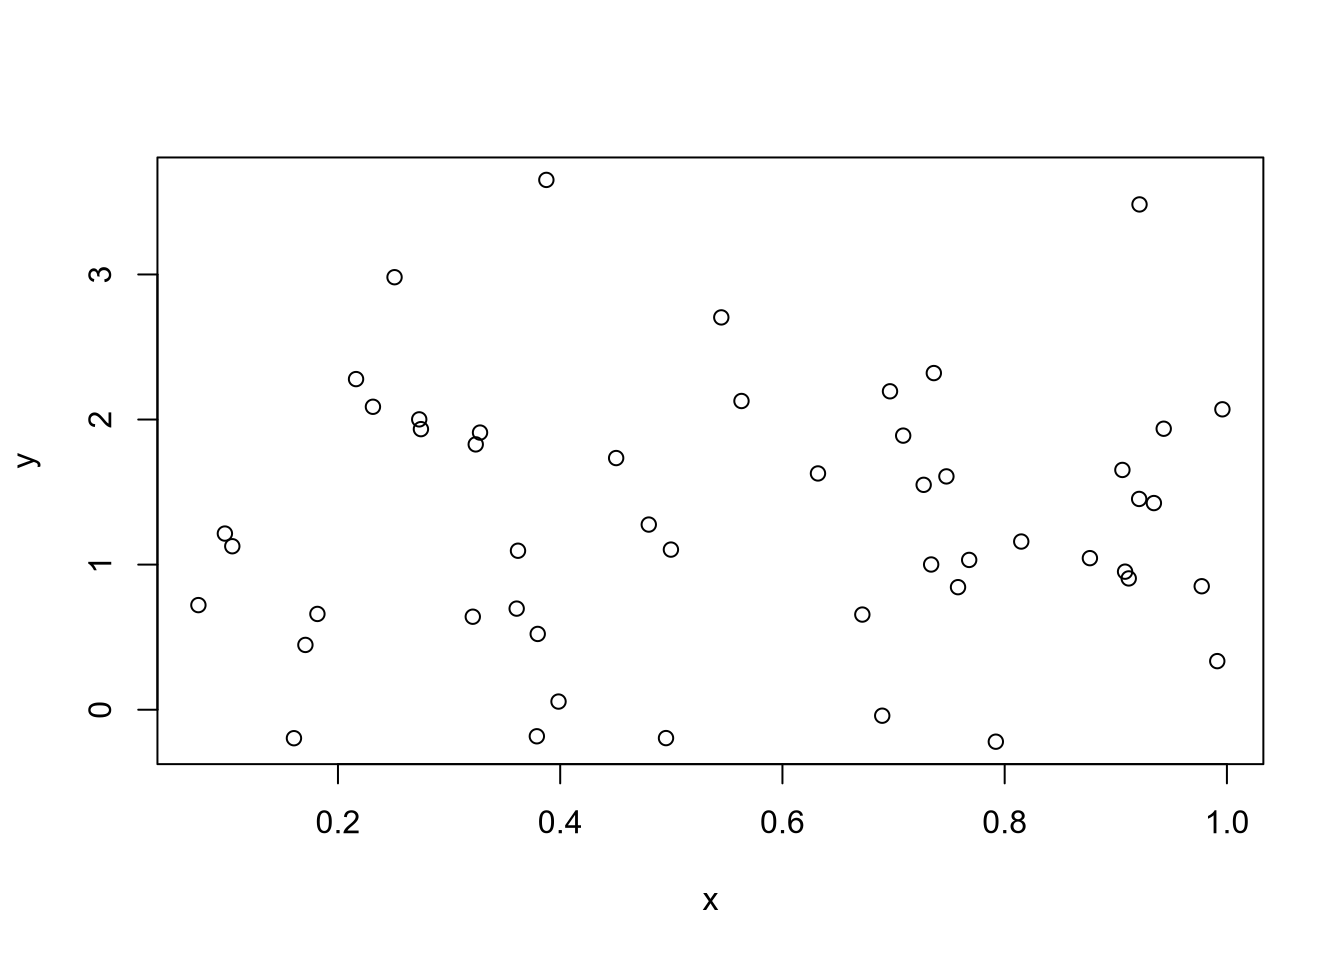
\includegraphics{pdaps_files/figure-latex/unnamed-chunk-9-1.pdf}

We know the true slope is non-zero, though with such a small effect and such a small sample it's hard to tell from the scatterplot.

We can run a regression of \(Y\) on \(X\) and extract the estimated slope and its \(p\)-value (for a test of \(H_0 : \beta = 0\)).

\begin{Shaded}
\begin{Highlighting}[]
\KeywordTok{library}\NormalTok{(}\StringTok{"tidyverse"}\NormalTok{)}
\KeywordTok{library}\NormalTok{(}\StringTok{"broom"}\NormalTok{)}

\NormalTok{fit \textless{}{-}}\StringTok{ }\KeywordTok{lm}\NormalTok{(y }\OperatorTok{\textasciitilde{}}\StringTok{ }\NormalTok{x)}
\KeywordTok{tidy}\NormalTok{(fit)  }\CommentTok{\# Full regression table}
\end{Highlighting}
\end{Shaded}

\begin{verbatim}
## # A tibble: 2 x 5
##   term        estimate std.error statistic  p.value
##   <chr>          <dbl>     <dbl>     <dbl>    <dbl>
## 1 (Intercept)    1.22      0.289     4.22  0.000108
## 2 x              0.177     0.460     0.386 0.702
\end{verbatim}

\begin{Shaded}
\begin{Highlighting}[]
\KeywordTok{tidy}\NormalTok{(fit)[}\DecValTok{2}\NormalTok{, }\KeywordTok{c}\NormalTok{(}\StringTok{"estimate"}\NormalTok{, }\StringTok{"p.value"}\NormalTok{)]  }\CommentTok{\# Parts we want}
\end{Highlighting}
\end{Shaded}

\begin{verbatim}
## # A tibble: 1 x 2
##   estimate p.value
##      <dbl>   <dbl>
## 1    0.177   0.702
\end{verbatim}

This just gives us one instance of what we would get from this type of sample from this particular model. What we're really interested in, though, is the \emph{sampling distribution}---the distribution of results we would get across many samples from this model. More specifically, we want to answer two questions.

\begin{enumerate}
\def\labelenumi{\arabic{enumi}.}
\item
  If the results of every sample from this model were made public, what would we infer from the full body of evidence?
\item
  If only the statistically significant results were made public, what we infer from the published body of evidence?
\end{enumerate}

To make that task a bit simpler, let's write a function that collects everything we just did: generates a sample of size \texttt{n\_obs}, runs a regression of \(Y\) on \(X\), and spits back the estimated slope and its \(p\)-value.

\begin{Shaded}
\begin{Highlighting}[]
\NormalTok{draw\_slope\_and\_p \textless{}{-}}\StringTok{ }\ControlFlowTok{function}\NormalTok{(n\_obs) \{}
\NormalTok{    x \textless{}{-}}\StringTok{ }\KeywordTok{runif}\NormalTok{(n\_obs, }\DataTypeTok{min =} \DecValTok{0}\NormalTok{, }\DataTypeTok{max =} \DecValTok{1}\NormalTok{)}
\NormalTok{    y \textless{}{-}}\StringTok{ }\DecValTok{1} \OperatorTok{+}\StringTok{ }\FloatTok{0.5} \OperatorTok{*}\StringTok{ }\NormalTok{x }\OperatorTok{+}\StringTok{ }\KeywordTok{rnorm}\NormalTok{(n\_obs, }\DataTypeTok{mean =} \DecValTok{0}\NormalTok{, }\DataTypeTok{sd =} \DecValTok{1}\NormalTok{)}
\NormalTok{    fit \textless{}{-}}\StringTok{ }\KeywordTok{lm}\NormalTok{(y }\OperatorTok{\textasciitilde{}}\StringTok{ }\NormalTok{x)}
\NormalTok{    out \textless{}{-}}\StringTok{ }\KeywordTok{tidy}\NormalTok{(fit)[}\DecValTok{2}\NormalTok{, }\KeywordTok{c}\NormalTok{(}\StringTok{"estimate"}\NormalTok{, }\StringTok{"p.value"}\NormalTok{)]}
    \KeywordTok{as.numeric}\NormalTok{(out)  }\CommentTok{\# Convert data frame to vector}
\NormalTok{\}}
\end{Highlighting}
\end{Shaded}

Since this function is drawing random numbers, it will return different results every time we run it.

\begin{Shaded}
\begin{Highlighting}[]
\KeywordTok{draw\_slope\_and\_p}\NormalTok{(}\DecValTok{50}\NormalTok{)}
\end{Highlighting}
\end{Shaded}

\begin{verbatim}
## [1] 0.3873035 0.3692928
\end{verbatim}

\begin{Shaded}
\begin{Highlighting}[]
\KeywordTok{draw\_slope\_and\_p}\NormalTok{(}\DecValTok{50}\NormalTok{)}
\end{Highlighting}
\end{Shaded}

\begin{verbatim}
## [1] 0.212866 0.674392
\end{verbatim}

Now what we want to do is to run this function a whole bunch of times, say 1,000. That lets us imagine what would happen if 1,000 different labs each took a different sample of size \(N = 50\) from the population, estimated the slope of the regression line, and tested against the null hypothesis that the slope is zero. To do that, we can use the \texttt{replicate()} function, which is a convenient way to run the same function repeatedly.

\begin{Shaded}
\begin{Highlighting}[]
\NormalTok{results\_}\DecValTok{50}\NormalTok{ \textless{}{-}}\StringTok{ }\KeywordTok{replicate}\NormalTok{(}\DecValTok{1000}\NormalTok{, }\KeywordTok{draw\_slope\_and\_p}\NormalTok{(}\DecValTok{50}\NormalTok{))}
\KeywordTok{dim}\NormalTok{(results\_}\DecValTok{50}\NormalTok{)}
\end{Highlighting}
\end{Shaded}

\begin{verbatim}
## [1]    2 1000
\end{verbatim}

This gives us a \(2 \times 1000\) matrix. Each column is a separate run of \texttt{draw\_slope\_and\_p()}. The first row is the estimated slope; the second row is the associated \(p\)-value.

First let's check how often we rejected the null hypothesis. The null hypothesis is false, so we would ideally always reject it. However, we have a small effect size and each individual sample is small, so the effect is hard to detect in any given sample---we will often fail to reject the null hypothesis. Let's see exactly how often.

\begin{Shaded}
\begin{Highlighting}[]
\CommentTok{\# Proportion of p{-}values at or below 0.05}
\NormalTok{sig\_}\DecValTok{50}\NormalTok{ \textless{}{-}}\StringTok{ }\NormalTok{results\_}\DecValTok{50}\NormalTok{[}\DecValTok{2}\NormalTok{, ] }\OperatorTok{\textless{}=}\StringTok{ }\FloatTok{0.05}
\KeywordTok{mean}\NormalTok{(sig\_}\DecValTok{50}\NormalTok{)}
\end{Highlighting}
\end{Shaded}

\begin{verbatim}
## [1] 0.16
\end{verbatim}

So the power of our study is not great---most of the time, we're failing to reject the null hypothesis.

Let's see what the average estimated slope is across the full set of samples.

\begin{Shaded}
\begin{Highlighting}[]
\KeywordTok{mean}\NormalTok{(results\_}\DecValTok{50}\NormalTok{[}\DecValTok{1}\NormalTok{, ])}
\end{Highlighting}
\end{Shaded}

\begin{verbatim}
## [1] 0.5205715
\end{verbatim}

This is pretty close to the true value, reflecting the fact that OLS is unbiased. If all 1,000 studies were made public, we would ultimately infer---correctly---that the population slope is roughly 0.5.

But what if we only saw the small fraction of studies whose results were statistically significant?

\begin{Shaded}
\begin{Highlighting}[]
\CommentTok{\# Restrict to columns where p \textless{}= 0.05}
\KeywordTok{mean}\NormalTok{(results\_}\DecValTok{50}\NormalTok{[}\DecValTok{1}\NormalTok{, sig\_}\DecValTok{50}\NormalTok{])}
\end{Highlighting}
\end{Shaded}

\begin{verbatim}
## [1] 1.210619
\end{verbatim}

We might be tempted to trust these studies more, since they are the ones that correctly reject the null hypothesis. But in fact, if we throw away those that are statistically insignificant, we end up with a biased picture of the effect size. The average effect size in the significant studies is more than double the true effect size. We can see this if we compare the distribution of all results to that of just the significant results.

\begin{Shaded}
\begin{Highlighting}[]
\KeywordTok{hist}\NormalTok{(results\_}\DecValTok{50}\NormalTok{[}\DecValTok{1}\NormalTok{, ])}
\end{Highlighting}
\end{Shaded}

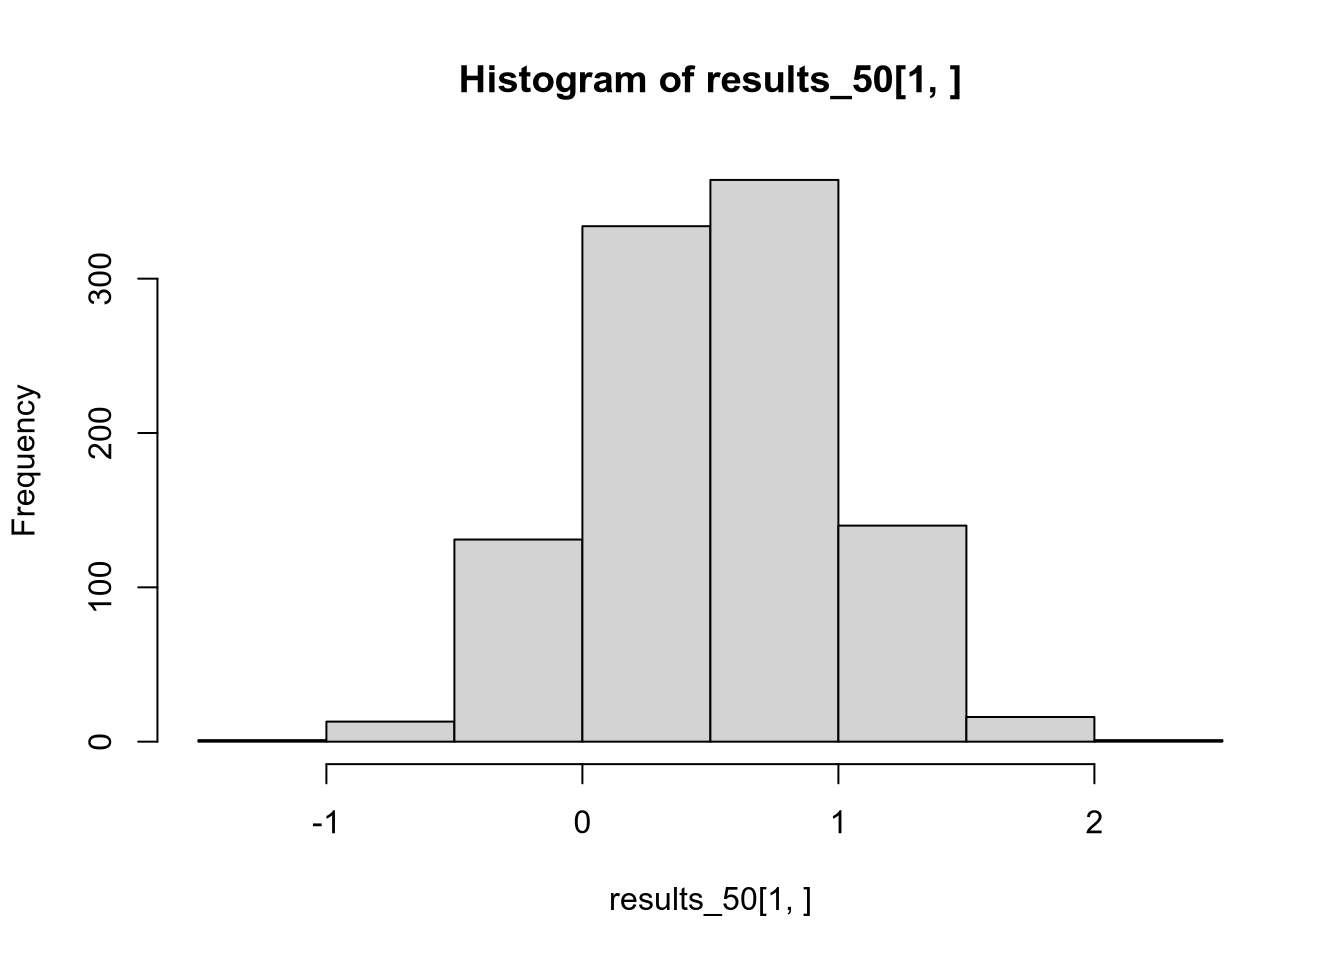
\includegraphics{pdaps_files/figure-latex/unnamed-chunk-17-1.pdf}

\begin{Shaded}
\begin{Highlighting}[]
\KeywordTok{hist}\NormalTok{(results\_}\DecValTok{50}\NormalTok{[}\DecValTok{1}\NormalTok{, sig\_}\DecValTok{50}\NormalTok{])}
\end{Highlighting}
\end{Shaded}

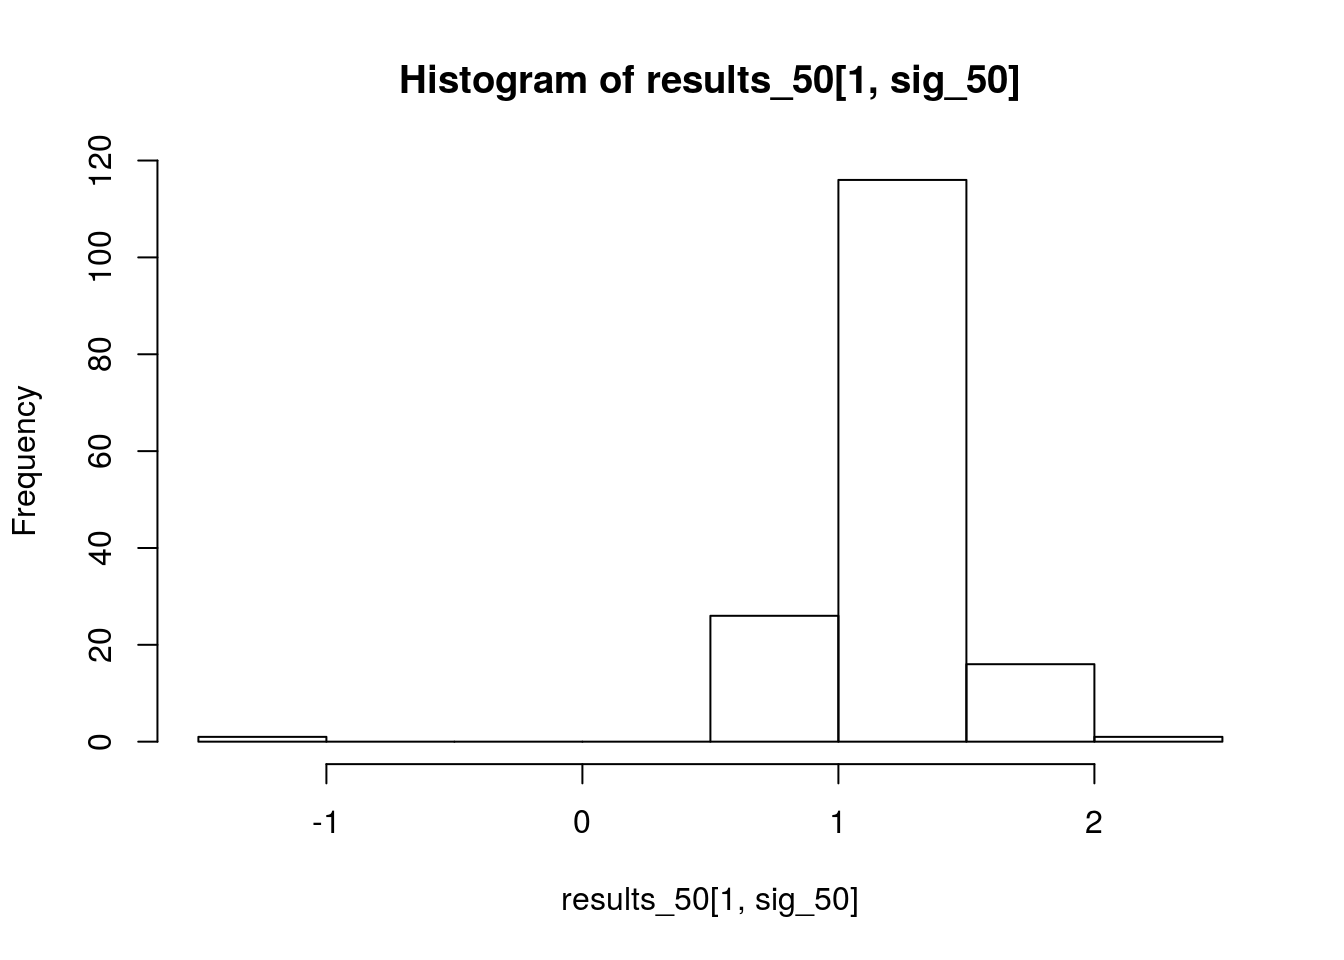
\includegraphics{pdaps_files/figure-latex/unnamed-chunk-17-2.pdf}

We can also see that this problem stems in large part from low statistical power. Suppose each lab were taking a sample of \(N = 200\) instead of \(N = 50\), making their effect estimates more precise and thereby increasing each lab's chance of (correctly) rejecting the null hypothesis.

\begin{Shaded}
\begin{Highlighting}[]
\NormalTok{results\_}\DecValTok{200}\NormalTok{ \textless{}{-}}\StringTok{ }\KeywordTok{replicate}\NormalTok{(}\DecValTok{1000}\NormalTok{, }\KeywordTok{draw\_slope\_and\_p}\NormalTok{(}\DecValTok{200}\NormalTok{))}
\NormalTok{sig\_}\DecValTok{200}\NormalTok{ \textless{}{-}}\StringTok{ }\NormalTok{results\_}\DecValTok{200}\NormalTok{[}\DecValTok{2}\NormalTok{, ] }\OperatorTok{\textless{}=}\StringTok{ }\FloatTok{0.05}

\CommentTok{\# Power}
\KeywordTok{mean}\NormalTok{(sig\_}\DecValTok{200}\NormalTok{)}
\end{Highlighting}
\end{Shaded}

\begin{verbatim}
## [1] 0.535
\end{verbatim}

\begin{Shaded}
\begin{Highlighting}[]
\CommentTok{\# Average estimate through the significance filter}
\KeywordTok{mean}\NormalTok{(results\_}\DecValTok{200}\NormalTok{[}\DecValTok{1}\NormalTok{, sig\_}\DecValTok{200}\NormalTok{])}
\end{Highlighting}
\end{Shaded}

\begin{verbatim}
## [1] 0.6740676
\end{verbatim}

\begin{Shaded}
\begin{Highlighting}[]
\KeywordTok{hist}\NormalTok{(results\_}\DecValTok{200}\NormalTok{[}\DecValTok{1}\NormalTok{, sig\_}\DecValTok{200}\NormalTok{])}
\end{Highlighting}
\end{Shaded}

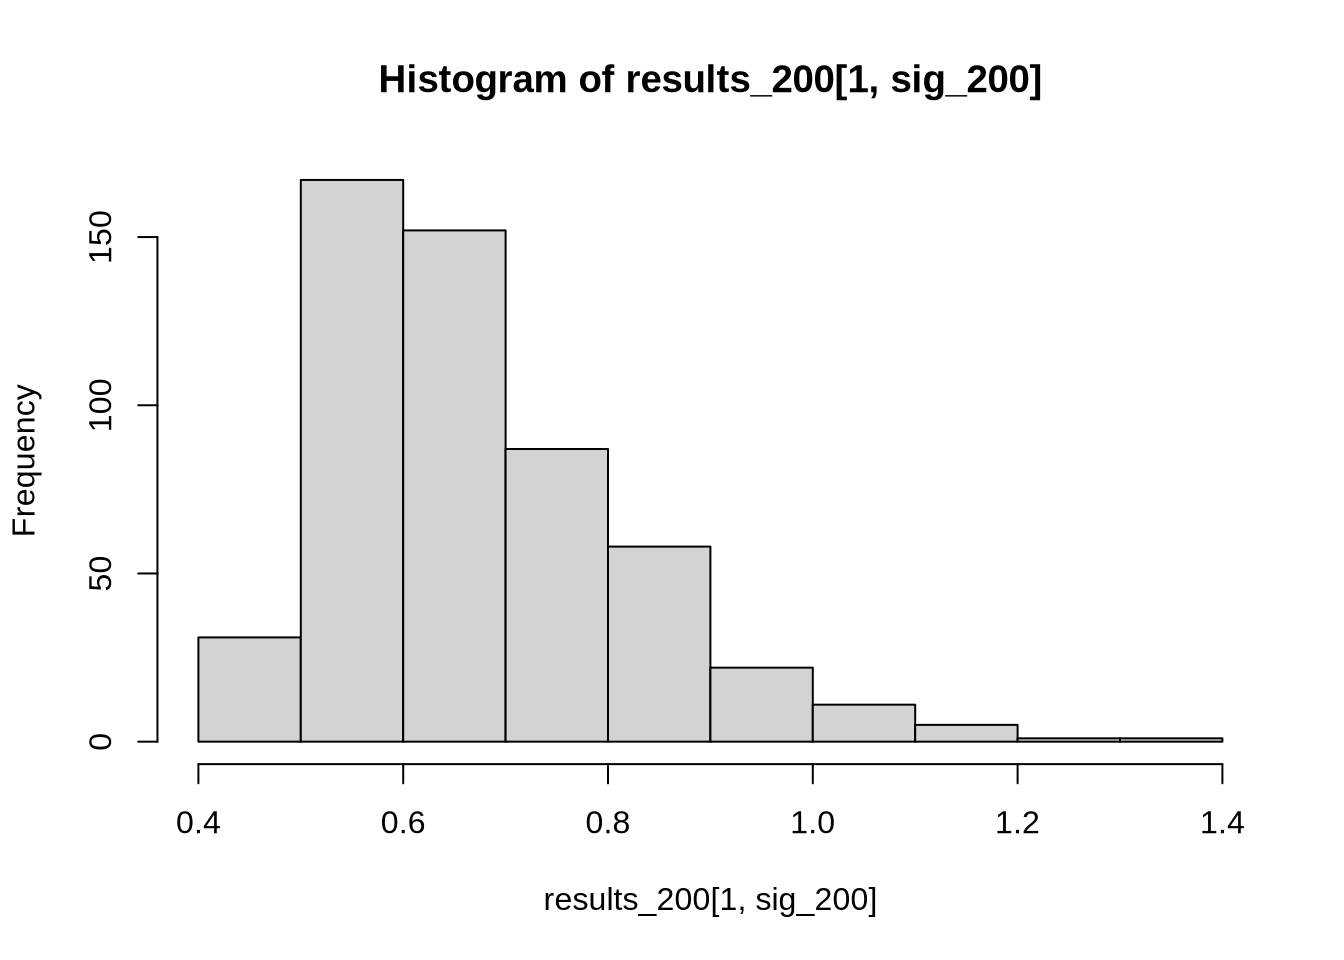
\includegraphics{pdaps_files/figure-latex/unnamed-chunk-19-1.pdf}

The significance-filtered average is still overinflated, but not nearly as drastically as when we were working with a small sample.

\hypertarget{panel}{%
\chapter{Clustered and Panel Data}\label{panel}}

Grouped data structures, in which we observe individual units within larger groups, are common in political science and other social sciences. Examples include:

\begin{itemize}
\item
  Cross-national survey data, where we observe individual respondents grouped by country.
\item
  Block-randomized field experiments. For example, in an experiment where the treatment is administered at the village level, we observe individual outcomes grouped by village.
\item
  Panel data, where we observe the same units repeatedly over time. This includes panel surveys as well as observational data on states, countries, or other political units over time.
\end{itemize}

Grouped data presents problems and opportunities. At the root of both is the idea of \emph{unobserved heterogeneity}---that some variation across groups might be due to unobservable features of the groups.

To return to our running example, suppose you are interested in the correlates of voting for Donald Trump in the 2016 general election. You observe survey respondents grouped by state. Vote choice might be affected by:

\begin{enumerate}
\def\labelenumi{\arabic{enumi}.}
\item
  \emph{Individual} characteristics like one's age, gender, race, income, and education.
\item
  \emph{State} characteristics\footnote{Why did I leave out national characteristics, like inflation or the national unemployment rate? In a single-election study, these are constant. While they might shape variation \emph{across} elections, they cannot be linked to variation \emph{within} a single election.} like the unemployment rate, undocumented population, and exposure to trade with China.
\end{enumerate}

Some state characteristics that might affect vote choice are difficult or impossible to measure. For example, some states have a more cosmopolitan culture, while others have a more traditional culture. A 50-year-old white man living in Connecticut is, we would expect, less likely to have voted for Trump than a 50-year-old white man living in Alabama. This is \emph{unobserved heterogeneity}---characteristics that we do not observe, and therefore cannot control for, but which affect the response.

If we are not careful in dealing with grouped data, unobserved heterogeneity can be a major problem. The spherical errors assumption is usually not tenable for grouped data, since observations will be correlated with others in the same group. OLS will therefore be inefficient and yield invalid inferences. Even worse, if group-level sources of unobserved heterogeneity are correlated with individual characteristics---if, say, younger voters are more likely to live in cosmopolitan states---OLS may also be biased and inconsistent.

On the other hand, if we deal with grouped data properly, we can enhance the credibility of our inferences. We can eliminate the influence of variation \emph{across} groups, allowing us to focus on the comparisons \emph{within} groups that we are usually most interested in.

Before we get started, a note of caution. We only have enough time to scratch the surface of how to analyze grouped data. If you work with grouped data in your dissertation or other research, you should think carefully about your data structure and potential sources of unobserved heterogeneity. The methods we discuss this week may not solve your problems. As further references, I recommend \citet{Wooldridge:2002vr} and \citet{gelman2006data}.

\hypertarget{the-linear-model-with-grouped-data}{%
\section{The Linear Model with Grouped Data}\label{the-linear-model-with-grouped-data}}

We need to change our notation a bit to reflect the arrangement of observations into groups. Let there be \(G\) groups indexed by \(g = 1, \ldots, G\). Within each group, we have \(N\) observations indexed by \(n = 1, \ldots, N\).\footnote{Everything we do here would go through if we allowed the number of observations to vary across groups, but the notation would get uglier. In the panel data context we say that the panels are \emph{balanced} if the number of observations is the same for each group and \emph{unbalanced} otherwise.} (In the special case of panel data, where each group is a unit observed over time, the standard notation is to use \(t = 1, \ldots, T\) instead.)

We will now index individual ``rows'' of the data by \(gn\), which stands for the \(n\)'th observation within group \(g\).

\begin{itemize}
\tightlist
\item
  Unit-level

  \begin{itemize}
  \tightlist
  \item
    \(Y_{gn}\): response for the \(gn\)'th observation
  \item
    \(\mathbf{x}_{gn}\): vector of \(K\) covariates for the \(gn\)'th observation
  \item
    \(\epsilon_{gn}\): random shock to the \(gn\)'th response
  \end{itemize}
\item
  Group-level

  \begin{itemize}
  \tightlist
  \item
    \(\mathbf{Y}_g\): vector of \(N\) responses for the \(g\)'th group
  \item
    \(\mathbf{X}_g\): \(N \times K\) matrix of covariates for the \(g\)'th group
  \item
    \(\epsilon_g\): vector of \(N\) random shocks for the \(g\)'th group
  \end{itemize}
\item
  Full data

  \begin{itemize}
  \tightlist
  \item
    \(\mathbf{Y}\): vector of all \(GN\) responses, where \[\mathbf{Y} = \begin{bmatrix} \mathbf{Y}_1 \\ \mathbf{Y}_2 \\ \vdots \\ \mathbf{Y}_G \end{bmatrix}.\]
  \item
    \(\mathbf{X}\): \(GN \times K\) matrix of covariates, where \[\mathbf{X} = \begin{bmatrix} \mathbf{X}_1 \\ \mathbf{X}_2 \\ \vdots \\ \mathbf{X}_G \end{bmatrix}.\]
  \item
    \(\mathbf{D}\): \(GN \times G\) matrix of group membership indicators.
  \item
    \(\epsilon\): vector of all \(GN\) random shocks
  \end{itemize}
\end{itemize}

If we assume a standard linear model for each \(gn\)'th response,
\[
Y_{gn} = \mathbf{x}_{gn} \cdot \beta + \epsilon_{gn},
\]
we end up with the familiar matrix equation
\[
\mathbf{Y} = \mathbf{X} \beta + \epsilon.
\]

You may look at this equation and think, ``This looks like something we've used OLS on. What's wrong with OLS?'' Two reasons. First, at a minimum, we are unlikely to have spherical errors in grouped data. Observations in the same group---students in the same classroom, voters in the same state, LAPOP respondents in the same country---are likely to have residual correlation. There are unmeasured factors that commonly affect their responses. As in any non-spherical error model, this means OLS will yield invalid inferences. Moreover, because we are talking about autocorrelation and not just heteroskedasticity, White's heteroskedasticity-consistent standard errors won't do the trick.

Second, depending on the nature of the group-specific effects, we may also have a failure of strict exogeneity. I hope I have impressed on you by now that this is a major problem. To see why we have a failure of strict exogeneity, let us return to the example of voters living in states with cosmopolitan versus traditional cultures. If we cannot measure cosmopolitanism (as I am assuming), then it ends up in the error term of our model:
\[
\epsilon_{gn} = \text{Cosmpolitanism}_g + \text{Other Stuff}_{gn}.
\]
But we know that younger and more educated voters are more likely to live in cosmopolitan areas. So if our covariate matrix includes age and education, we have
\[
E[\epsilon \,|\, \mathbf{X}] \neq \mathbf{0}.
\]

We will proceed from the easiest problems to the hardest. We will first consider a standard error correction and an efficiency improvement for the case where errors are correlated within groups but strict exogeneity still holds. We will then identify an unbiased estimator in the case where strict exogeneity fails.

\hypertarget{autocorrelation-within-groups}{%
\section{Autocorrelation within Groups}\label{autocorrelation-within-groups}}

\providecommand{\Cor}{\mathop{\rm Cor}\nolimits}
\providecommand{\se}{\mathop{\rm se}\nolimits}

Imagine the following policy experiment. The federal government randomly selects half of the states to receive a grant intended to improve high school education, while the other half do not receive it. We observe some indicator of educational quality (e.g., graduation rates) at the school district level, where school districts are grouped within states. So our model looks like
\[
\text{Quality}_{gn} = \beta_1 + \beta_2 \text{Grant}_g + \epsilon_{gn}.
\]
We want to know whether receiving the grant affected quality. What we cannot measure is how well the states used the money. If some states used it better than others, then we would expect the error term to be correlated across school districts within the state. In a state where the money was used wisely, we would expect most of the schools to do ``better than expected''---to have positive residuals, in the language of regression. Conversely, in a state where the money was squandered, we would expect most of the schools to do worse than we would otherwise predict.

This is one example of the general phenomenon Moulton \citetext{\citeyear{Moulton:1986kw}; \citeyear{Moulton:1990bl}} identifies---that there is often substantial correlation in the random errors within groups, especially when we are looking at the effects of variables that only vary at the group level. One way I think about it is that, with grouped data and group-level covariates, the effective number of observations is less than the nominal number of observations. If we use the OLS standard errors, we are pretending to have more data than we really do.

Let's see a bit more formally why autocorrelation within groups would cause us to overstate the effective sample size.
Imagine we have \(N = 4\) observations organized into \(G = 2\) groups, with the groups being the first two and last two observations respectively.
Furthermore, let's assume we have a single covariate that varies across groups but not within them (e.g., a random treatment assigned at the group level), so that our data matrix looks like
\[
\mathbf{X} = \begin{bmatrix}
1 & x_1 \\
1 & x_1 \\
1 & x_2 \\
1 & x_2
\end{bmatrix}.
\]
Finally, assume the errors are homoskedastic but are autocorrelated within groups:

\begin{itemize}
\tightlist
\item
  \(V[\epsilon_n] = \sigma^2\) for all \(n\).
\item
  \(\mathop{\rm Cor}\nolimits[\epsilon_1, \epsilon_2] = \mathop{\rm Cor}\nolimits[\epsilon_3, \epsilon_4] = \rho\).
\item
  \(\mathop{\rm Cor}\nolimits[\epsilon_n, \epsilon_m] = 0\) for all other \(n, m\) pairs.
\end{itemize}

Then we can write the variance matrix of the error term as \(V[\epsilon \,|\, \mathbf{X}] = \sigma^2 \Omega\), where
\[
\Omega = \begin{bmatrix}
1 & \rho & 0 & 0 \\
\rho & 1 & 0 & 0 \\
0 & 0 & 1 & \rho \\
0 & 0 & \rho & 1
\end{bmatrix}.
\]

The OLS formula for the variance of the coefficients is \(V[\hat{\beta} \,|\, \mathbf{X}] = \sigma^2 (\mathbf{X}^\top \mathbf{X})^{-1}\).
However, we know that this formula is not appropriate in this case because the spherical errors assumption does not hold.
Remember that for a general error structure \(V[\epsilon \,|\, \mathbf{X}] = \sigma^2 \Omega\), the true variance of the OLS estimator is
\[
V[\hat{\beta} \,|\, \mathbf{X}]
= \sigma^2 \underbrace{(\mathbf{X}^\top \mathbf{X})^{-1}}_{\text{bread}} \underbrace{\mathbf{X}^\top \Omega \mathbf{X}}_{\text{meat}} \underbrace{(\mathbf{X}^\top \mathbf{X})^{-1}}_{\text{bread}}.
\]
In the present case, the ``meat'' of the above expression is
\[
\begin{aligned}
\mathbf{X}^\top \Omega \mathbf{X}
&= \begin{bmatrix}
1 & 1 & 1 & 1 \\
x_1 & x_1 & x_2 & x_2
\end{bmatrix}
\begin{bmatrix}
1 & \rho & 0 & 0 \\
\rho & 1 & 0 & 0 \\
0 & 0 & 1 & \rho \\
0 & 0 & \rho & 1
\end{bmatrix}
\begin{bmatrix}
1 & x_1 \\
1 & x_1 \\
1 & x_2 \\
1 & x_2
\end{bmatrix} \\
&= \begin{bmatrix}
1 + \rho & 1 + \rho & 1 + \rho & 1 + \rho \\
(1 + \rho) x_1 & (1 + \rho) x_1 & (1 + \rho) x_2 & (1 + \rho) x_2
\end{bmatrix}
\begin{bmatrix}
1 & x_1 \\
1 & x_1 \\
1 & x_2 \\
1 & x_2
\end{bmatrix} \\
&= (1 + \rho) \begin{bmatrix}
1 & 1 & 1 & 1 \\
x_1 & x_1 & x_2 & x_2
\end{bmatrix}
\begin{bmatrix}
1 & x_1 \\
1 & x_1 \\
1 & x_2 \\
1 & x_2
\end{bmatrix} \\
&= (1 + \rho) \mathbf{X}^\top \mathbf{X}.
\end{aligned}
\]
Therefore, we have
\[
\begin{aligned}
V[\hat{\beta} \,|\, \mathbf{X}]
&= \sigma^2 (\mathbf{X}^\top \mathbf{X})^{-1} \mathbf{X}^\top \Omega \mathbf{X} (\mathbf{X}^\top \mathbf{X})^{-1} \\
&= \sigma^2 (\mathbf{X}^\top \mathbf{X})^{-1} [(1 - \rho) \mathbf{X}^\top \mathbf{X}] (\mathbf{X}^\top \mathbf{X})^{-1} \\
&= \sigma^2 (1 - \rho) (\mathbf{X}^\top \mathbf{X})^{-1}.
\end{aligned}
\]
In other words, if we use the OLS formula in the presence of grouped autocorrelation, our standard errors will be too small by a factor of \(\sqrt{1 - \rho}\).

This is a special case of the \emph{Moulton factor} (see MHE 8.2.1).
If all groups have \(m\) observations, the covariate varies only at the group level, errors are homoskedastic, and the within-group correlation is \(\rho\) for all groups, then the OLS standard error calculation will underestimate the true standard errors by a factor of \(\sqrt{1 + (m - 1) \rho}\).
If for some reason we were certain the homoskedasticity assumption held \emph{and} we knew \(\rho\), then we could simply correct the OLS standard errors by applying this formula.
More broadly, if we knew the exact structure of heteroskedasticity and autocorrelation, we could obtain an efficient estimate of \(\beta\) and proper standard errors by using GLS.
Usually, however, this option will not be available to us.

\hypertarget{clustered-standard-errors}{%
\section{Clustered Standard Errors}\label{clustered-standard-errors}}

Luckily, we can correct ``clustered'' errors in a manner similar to what we did when encountering heteroskedasticity of unknown form. The most we can assume on \(\Omega = V[\epsilon \,|\, \mathbf{X}]\) is

\begin{itemize}
\item
  Heteroskedasticity of unknown form, within and across groups.
\item
  Autocorrelation of unknown form within groups.
\item
  \emph{No} autocorrelation across groups.
\end{itemize}

Under these assumptions, \(\Omega\) has the block-diagonal form
\[
\Omega = \begin{bmatrix}
  \Omega_1 & \mathbf{0} & \cdots & \mathbf{0} \\
  \mathbf{0} & \Omega_2 & \cdots & \mathbf{0} \\
  \vdots & \vdots & \ddots & \vdots \\
  \mathbf{0} & \mathbf{0} & \cdots & \Omega_G
\end{bmatrix},
\]
where each \(\Omega_g\) is a symmetric \(N \times N\) matrix. These may differ from each other---each group may have its own special autocorrelation structure.
Notice that this is more general than the assumptions under which we obtained the Moulton factor above.

If we knew \(\Omega\) exactly, we could use GLS to efficiently estimate \(\beta\) and obtain correct standard errors. That is unlikely. Instead, we will use OLS to obtain our coefficient estimates, then we will correct the standard errors so as to be approximately correct in large samples. The \emph{cluster-robust variance estimator} is
\[
\hat{\Sigma}_{\text{CR}} =
(\mathbf{X}^\top \mathbf{X})^{-1}
\left( \sum_{g=1}^G \mathbf{X}_g^\top \hat{e}_g \hat{e}_g^\top \mathbf{X}_g \right)
(\mathbf{X}^\top \mathbf{X})^{-1},
\]
where \(\hat{e}_g\) is the \(N \times 1\) vector of OLS residuals for the \(g\)'th group. Like White's estimator for heteroskedasticity, this is a ``sandwich'' estimator. The ``meat'' of the sandwich here accounts for the within-group correlations in the error term.

Also like White's estimator for heteroskedasticity, the cluster-robust estimator is consistent, but not unbiased. It approaches the truth as \(G\), the number of groups, grows large (holding fixed \(N\), the number of observations per group), but it may be badly biased in small samples. The consensus seems to be that \(N = 50\) is large enough \citep{Cameron:2015ud}, so you Americanists may go ahead and rejoice. However, if you observe a small number of units over a long period of time (e.g., in a study of the historical political economy of Western European countries), the cluster-robust standard error estimator will be severely biased. \citet{Beck:1995hm} provide a similar estimator for such data, except with the summation in the middle of the ``sandwich'' taken over the \(N\) time periods instead of the \(G\) groups.

The earliest derivation of this estimator was \citet{Liang:1986gv}, and that is whom you should cite when you use it. \citet{Arellano:1987jx} derives the same estimator but is a bit easier to follow. As with White's estimator, there are various finite-sample corrections to \(\hat{\Sigma}_{\text{CR}}\) that you may want to use; we will not go through those here.

\hypertarget{random-effects}{%
\section{Random Effects}\label{random-effects}}

\emph{The coverage and notation in this section and the next one closely follow \citet[chapter 12]{Johnston:1997um}.}

Just as Huber-White standard errors do not fix the inefficiency of OLS under heteroskedasticity, cluster-robust standard errors do not fix the inefficiency of OLS under within-group correlation. To get a handle on the efficiency problem, we will make further assumptions about the source of that correlation.

We will assume each group \(g\) has a (potentially) different intercept. We can incorporate this into our original model,
\[
Y_{gn} = \mathbf{x}_{gn} \cdot \beta + \epsilon_{gn},
\]
by decomposing the error term into independent \emph{group-specific} and \emph{individual-specific} components:
\[
\epsilon_{gn} = \underbrace{\alpha_g}_{\text{group}} + \underbrace{\eta_{gn}}_{\text{individual}}.
\]
In this equation, \(\alpha_g\) represents the difference between the intercept for group \(g\) and the overall average, while \(\eta_{gn}\) is an idiosyncratic shock specific to the \(n\)'th observation of group \(g\). We will assume that \(\eta_{gn}\) is independent and identically distributed across observations, so that the only source of autocorrelation is that observations in the same group share the same \(\alpha_g\).

When we decompose the error term like this, we are assuming implicitly that the \(\alpha_g\)'s are uncorrelated with the covariates in the model. Otherwise, strict exogeneity fails and the techniques that follow are useless. Let me put that another way---the random effects model depends on the assumption that the group-specific shocks are uncorrelated with the covariates. We will proceed under this assumption, and return shortly to the questions of testing it and what to do if it fails.

The random-intercepts model gives us a convenient structure for the \(\Omega\) matrix in GLS. Let \(V[\alpha_g] = \sigma^2_\alpha\) and \(V[\eta_{gn}] = \sigma^2_\eta\). The error variance matrix for the \(g\)'th group then works out to
\[
\Omega_g = \begin{bmatrix}
\sigma_{\eta}^2 + \sigma_{\alpha}^2 & \sigma_{\alpha}^2 & \cdots & \sigma_{\alpha}^2 \\
\sigma_{\alpha}^2 & \sigma_{\eta}^2 + \sigma_{\alpha}^2 & \cdots & \sigma_{\alpha}^2 \\
\vdots & \vdots & \ddots & \vdots \\
\sigma_{\alpha}^2 & \sigma_{\alpha}^2 & \cdots & \sigma_{\eta}^2 + \sigma_{\alpha}^2
\end{bmatrix}.
\]
Since there is no autocorrelation across groups, \(\Omega\) takes the same block-diagonal form as in our discussion of cluster-robust standard errors.

If we knew \(\sigma^2_\alpha\) and \(\sigma^2_\eta\), we could estimate \(\beta\) by GLS. It is unlikely, however, that we would know these in advance. Luckily, there is a compromise option available. \emph{Feasible GLS}, or FGLS, entails using a pair of first-stage regressions to estimate the variance of \(\alpha\) and \(\eta\), then plugging these into the GLS formula.

There are many ways to estimate these variances.
In practice, this isn't a problem you'll need to worry about, since the variance estimates will be computed behind the scenes by your statistical software.
But I think it's useful to have a basic understanding of what's going on when you use random effects, so here is one simple way to estimate \(\sigma^2_\alpha\) and \(\sigma^2_\eta\).

\begin{enumerate}
\def\labelenumi{\arabic{enumi}.}
\item
  Run OLS of \(\mathbf{Y}\) on \(\mathbf{X}\).
  Let \(\hat{\sigma}^2\) denote the estimated residual variance from this ``pooled model''---so called because it ignores group-level variation, throwing all the observations into a single pool.
  This is a consistent estimator of the total residual variance, \(\sigma^2_\alpha + \sigma^2_\eta\).
\item
  Run OLS of \(\mathbf{Y}\) on \([\mathbf{X} \quad \mathbf{D}]\), i.e., the covariates plus a set of group membership indicators.
  This is the fixed effects regression, which we will talk about shortly.
  Because the group membership indicators account for variation \emph{across} groups, the remaining variation in this model solely represents variance \emph{within} groups.
  We can therefore let the estimated residual variance from this model be \(\hat{\sigma}^2_\eta\), which is a consistent estimator of the within-group variance, \(\sigma^2_\eta\).
\item
  Estimate the between-group variance as \(\hat{\sigma}^2_\alpha = \hat{\sigma}^2 - \hat{\sigma}^2_\eta\).
\item
  Form the matrix \(\hat{\Omega}\) by plugging \(\hat{\sigma}^2_\alpha\) and \(\hat{\sigma}^2_\eta\) into the formulas above, then run GLS using \(\hat{\Omega}\) as the weighting matrix.
\end{enumerate}

This gives us the \emph{random effects estimator},
\[
\hat{\beta}_{\text{RE}} = (\mathbf{X}^\top \hat{\Omega}^{-1} \mathbf{X})^{-1} \mathbf{X}^\top \hat{\Omega}^{-1} \mathbf{Y}.
\]

See \citet[392--395]{Johnston:1997um} for full formulas and details. FGLS is consistent but not unbiased, so the random effects model may not be a good idea in small samples. If our specification of the error structure is correct, it is asymptotically efficient---as the sample size increases, no other estimator has lower standard errors.

\hypertarget{fixed-effects}{%
\section{Fixed Effects}\label{fixed-effects}}

What if the group-specific intercepts are correlated with the covariates? Then, in order to maintain strict exogeneity, we must pull them out of the error term and into the covariate matrix. This is easy to do---we can rewrite the full model as
\[
\mathbf{Y} = \mathbf{X} \beta + \mathbf{D} \alpha + \eta,
\]
where \(\alpha\) is the \(G \times 1\) vector of group-specific intercepts. This suggests that we run OLS on our covariates plus the full set of group membership indicators. (As with any set of indicators, we need to omit one category.) The first \(K\) elements of this regression constitute the \emph{fixed effects} estimator.

Most textbook treatments of fixed effect estimators go through a whole rigmarole about computation, because it used to be challenging to invert a \((K + G) \times (K + G)\) matrix when \(G\) was moderately large. This is no longer true,\footnote{When I taught this class last year, I simulated a dataset with a single covariate, \(N = 1{,}000\), and \(J = 1{,}000\), meaning the fixed effects regression entailed estimating \(1{,}001\) parameters from \(1{,}000{,}000\) observations. It took less than two minutes to run on my not-especially-powerful laptop. That said, should you ever have \(N\) another order of magnitude above that, the computational tricks given in the textbook treatments will once again be of use.} so you can safely ignore most of the hand-wringing about computational difficulties.

The standard errors of the fixed effects estimator are usually higher than those of the random effects estimator, since estimating \(G\) additional parameters uses a lot of degrees of freedom. This leads us to the following pair of observations.

\begin{itemize}
\item
  If the random effects assumption is met (group-specific effects are uncorrelated with covariates), then the random effects and fixed estimators are both consistent, but fixed effects is less efficient.
\item
  If the random effects assumption is not met, then the random effects estimator is inconsistent while the fixed effects estimator is consistent.
\end{itemize}

The typical test for whether fixed effects are necessary comes from \citet{Hausman:1978bi}. Under the null hypothesis that both estimators are consistent (and thus fixed effects are unnecessary and inefficient), the test statistic
\[
H = (\hat{\beta}_{\text{RE}} - \hat{\beta}_{\text{FE}})^\top (\hat{\Sigma}_{\text{FE}} - \hat{\Sigma}_{\text{RE}})^{-1} (\hat{\beta}_{\text{RE}} - \hat{\beta}_{\text{FE}})
\]
asymptotically has a \(\chi^2\) distribution with \(K\) degrees of freedom.

The other main drawback of fixed effects estimation is that you cannot estimate the effects of variables that do not vary within groups. (Why not?) See \citet[section 13.5]{greene} for estimation strategies with panel data and time-invariant covariates.

One final note: \citet{Arellano:1987jx} shows that the cluster-robust variance matrix estimator can be used with fixed effects. \citet{Cameron:2015ud} recommend doing so, at least when the number of groups is large.

\hypertarget{appendix-implementation-in-r-1}{%
\section{Appendix: Implementation in R}\label{appendix-implementation-in-r-1}}

The methods introduced here can be implemented via the \textbf{plm} package.

\begin{Shaded}
\begin{Highlighting}[]
\KeywordTok{library}\NormalTok{(}\StringTok{"plm"}\NormalTok{)}
\end{Highlighting}
\end{Shaded}

We will use the \texttt{Produc} dataset from \textbf{plm}, a riveting collection of economic statistics about the U.S. states from 1970 to 1986.

\begin{Shaded}
\begin{Highlighting}[]
\KeywordTok{data}\NormalTok{(Produc, }\DataTypeTok{package =} \StringTok{"plm"}\NormalTok{)}
\KeywordTok{head}\NormalTok{(Produc)}
\end{Highlighting}
\end{Shaded}

\begin{verbatim}
##     state year region     pcap     hwy   water    util       pc   gsp    emp
## 1 ALABAMA 1970      6 15032.67 7325.80 1655.68 6051.20 35793.80 28418 1010.5
## 2 ALABAMA 1971      6 15501.94 7525.94 1721.02 6254.98 37299.91 29375 1021.9
## 3 ALABAMA 1972      6 15972.41 7765.42 1764.75 6442.23 38670.30 31303 1072.3
## 4 ALABAMA 1973      6 16406.26 7907.66 1742.41 6756.19 40084.01 33430 1135.5
## 5 ALABAMA 1974      6 16762.67 8025.52 1734.85 7002.29 42057.31 33749 1169.8
## 6 ALABAMA 1975      6 17316.26 8158.23 1752.27 7405.76 43971.71 33604 1155.4
##   unemp
## 1   4.7
## 2   5.2
## 3   4.7
## 4   3.9
## 5   5.5
## 6   7.7
\end{verbatim}

The functions in \textbf{plm} assume that your data are organized like \texttt{Produc}, with the grouping variable in the first column and the identification variable (time, in the case of panel data) in the second column. See the \textbf{plm} package vignette on how to get datasets not organized this way into line.

We will treat unemployment (\texttt{unemp}) as our response and public capital stock (\texttt{pcap}) and private capital stock (\texttt{pc}) as our covariates. As a benchmark, let's use OLS.

\begin{Shaded}
\begin{Highlighting}[]
\NormalTok{fit\_ols \textless{}{-}}\StringTok{ }\KeywordTok{lm}\NormalTok{(unemp }\OperatorTok{\textasciitilde{}}\StringTok{ }\NormalTok{pcap }\OperatorTok{+}\StringTok{ }\NormalTok{pc,}
              \DataTypeTok{data =}\NormalTok{ Produc)}
\KeywordTok{summary}\NormalTok{(fit\_ols)}
\end{Highlighting}
\end{Shaded}

\begin{verbatim}
## 
## Call:
## lm(formula = unemp ~ pcap + pc, data = Produc)
## 
## Residuals:
##     Min      1Q  Median      3Q     Max 
## -3.5589 -1.6219 -0.3373  1.2129 11.5951 
## 
## Coefficients:
##              Estimate Std. Error t value Pr(>|t|)    
## (Intercept) 6.202e+00  1.077e-01  57.571   <2e-16 ***
## pcap        1.006e-05  5.515e-06   1.824   0.0686 .  
## pc          2.558e-06  2.563e-06   0.998   0.3186    
## ---
## Signif. codes:  0 '***' 0.001 '**' 0.01 '*' 0.05 '.' 0.1 ' ' 1
## 
## Residual standard error: 2.196 on 813 degrees of freedom
## Multiple R-squared:  0.03516,    Adjusted R-squared:  0.03279 
## F-statistic: 14.81 on 2 and 813 DF,  p-value: 4.795e-07
\end{verbatim}

The ``pooling'' estimator implemented by \texttt{plm()} ought to give us the same results.

\begin{Shaded}
\begin{Highlighting}[]
\NormalTok{fit\_pooling \textless{}{-}}\StringTok{ }\KeywordTok{plm}\NormalTok{(unemp }\OperatorTok{\textasciitilde{}}\StringTok{ }\NormalTok{pcap }\OperatorTok{+}\StringTok{ }\NormalTok{pc,}
                   \DataTypeTok{data =}\NormalTok{ Produc,}
                   \DataTypeTok{model =} \StringTok{"pooling"}\NormalTok{)}
\KeywordTok{summary}\NormalTok{(fit\_pooling)}
\end{Highlighting}
\end{Shaded}

\begin{verbatim}
## Pooling Model
## 
## Call:
## plm(formula = unemp ~ pcap + pc, data = Produc, model = "pooling")
## 
## Balanced Panel: n = 48, T = 17, N = 816
## 
## Residuals:
##     Min.  1st Qu.   Median  3rd Qu.     Max. 
## -3.55895 -1.62192 -0.33733  1.21292 11.59512 
## 
## Coefficients:
##               Estimate Std. Error t-value Pr(>|t|)    
## (Intercept) 6.2015e+00 1.0772e-01 57.5709  < 2e-16 ***
## pcap        1.0059e-05 5.5152e-06  1.8238  0.06855 .  
## pc          2.5582e-06 2.5633e-06  0.9980  0.31858    
## ---
## Signif. codes:  0 '***' 0.001 '**' 0.01 '*' 0.05 '.' 0.1 ' ' 1
## 
## Total Sum of Squares:    4064.6
## Residual Sum of Squares: 3921.7
## R-Squared:      0.035162
## Adj. R-Squared: 0.032788
## F-statistic: 14.8141 on 2 and 813 DF, p-value: 4.7947e-07
\end{verbatim}

We can obtain the cluster-robust variance matrix estimate via \texttt{vcovHC()}. Make sure to specify \texttt{method\ =\ "arellano"} so as to get the usual estimator. It is not entirely clear to me which of the various finite-sample adjustments corresponds to the defaults in Stata.

\begin{Shaded}
\begin{Highlighting}[]
\NormalTok{crvm\_pooling \textless{}{-}}\StringTok{ }\KeywordTok{vcovHC}\NormalTok{(fit\_pooling,}
                       \DataTypeTok{method =} \StringTok{"arellano"}\NormalTok{,}
                       \DataTypeTok{type =} \StringTok{"HC1"}\NormalTok{)}
\KeywordTok{summary}\NormalTok{(fit\_pooling, }\DataTypeTok{vcov =}\NormalTok{ crvm\_pooling)}
\end{Highlighting}
\end{Shaded}

\begin{verbatim}
## Pooling Model
## 
## Note: Coefficient variance-covariance matrix supplied: crvm_pooling
## 
## Call:
## plm(formula = unemp ~ pcap + pc, data = Produc, model = "pooling")
## 
## Balanced Panel: n = 48, T = 17, N = 816
## 
## Residuals:
##     Min.  1st Qu.   Median  3rd Qu.     Max. 
## -3.55895 -1.62192 -0.33733  1.21292 11.59512 
## 
## Coefficients:
##               Estimate Std. Error t-value Pr(>|t|)    
## (Intercept) 6.2015e+00 2.4475e-01 25.3385   <2e-16 ***
## pcap        1.0059e-05 1.2103e-05  0.8311   0.4062    
## pc          2.5582e-06 7.3044e-06  0.3502   0.7263    
## ---
## Signif. codes:  0 '***' 0.001 '**' 0.01 '*' 0.05 '.' 0.1 ' ' 1
## 
## Total Sum of Squares:    4064.6
## Residual Sum of Squares: 3921.7
## R-Squared:      0.035162
## Adj. R-Squared: 0.032788
## F-statistic: 6.45144 on 2 and 47 DF, p-value: 0.0033441
\end{verbatim}

Notice that our \(t\)-statistics are cut in more than half, even though our variables have within-group variation (unlike \citet{Moulton:1990bl}'s example).

We can also use \texttt{plm()} to estimate a random-effects model.

\begin{Shaded}
\begin{Highlighting}[]
\NormalTok{fit\_random \textless{}{-}}\StringTok{ }\KeywordTok{plm}\NormalTok{(unemp }\OperatorTok{\textasciitilde{}}\StringTok{ }\NormalTok{pcap }\OperatorTok{+}\StringTok{ }\NormalTok{pc,}
                  \DataTypeTok{data =}\NormalTok{ Produc,}
                  \DataTypeTok{model =} \StringTok{"random"}\NormalTok{)}
\KeywordTok{summary}\NormalTok{(fit\_random)}
\end{Highlighting}
\end{Shaded}

\begin{verbatim}
## Oneway (individual) effect Random Effect Model 
##    (Swamy-Arora's transformation)
## 
## Call:
## plm(formula = unemp ~ pcap + pc, data = Produc, model = "random")
## 
## Balanced Panel: n = 48, T = 17, N = 816
## 
## Effects:
##                 var std.dev share
## idiosyncratic 3.092   1.758  0.69
## individual    1.389   1.179  0.31
## theta: 0.6598
## 
## Residuals:
##     Min.  1st Qu.   Median  3rd Qu.     Max. 
## -3.65953 -1.35357 -0.28627  1.01012  9.72087 
## 
## Coefficients:
##               Estimate Std. Error z-value  Pr(>|z|)    
## (Intercept) 5.6656e+00 2.5521e-01 22.1996 < 2.2e-16 ***
## pcap        3.9178e-08 1.1236e-05  0.0035  0.997218    
## pc          1.6080e-05 4.5644e-06  3.5228  0.000427 ***
## ---
## Signif. codes:  0 '***' 0.001 '**' 0.01 '*' 0.05 '.' 0.1 ' ' 1
## 
## Total Sum of Squares:    2916.2
## Residual Sum of Squares: 2792.6
## R-Squared:      0.042399
## Adj. R-Squared: 0.040043
## Chisq: 35.9967 on 2 DF, p-value: 1.5256e-08
\end{verbatim}

And, finally, a fixed-effects model, which \texttt{plm()} calls the \texttt{"within"} model.

\begin{Shaded}
\begin{Highlighting}[]
\NormalTok{fit\_fixed \textless{}{-}}\StringTok{ }\KeywordTok{plm}\NormalTok{(unemp }\OperatorTok{\textasciitilde{}}\StringTok{ }\NormalTok{pcap }\OperatorTok{+}\StringTok{ }\NormalTok{pc,}
                 \DataTypeTok{data =}\NormalTok{ Produc,}
                 \DataTypeTok{model =} \StringTok{"within"}\NormalTok{)}
\KeywordTok{summary}\NormalTok{(fit\_fixed)}
\end{Highlighting}
\end{Shaded}

\begin{verbatim}
## Oneway (individual) effect Within Model
## 
## Call:
## plm(formula = unemp ~ pcap + pc, data = Produc, model = "within")
## 
## Balanced Panel: n = 48, T = 17, N = 816
## 
## Residuals:
##     Min.  1st Qu.   Median  3rd Qu.     Max. 
## -3.80687 -1.16760 -0.24813  0.94681  8.39430 
## 
## Coefficients:
##        Estimate Std. Error t-value  Pr(>|t|)    
## pcap 2.2699e-04 3.1813e-05  7.1352 2.244e-12 ***
## pc   4.1783e-06 6.5669e-06  0.6363    0.5248    
## ---
## Signif. codes:  0 '***' 0.001 '**' 0.01 '*' 0.05 '.' 0.1 ' ' 1
## 
## Total Sum of Squares:    2765.9
## Residual Sum of Squares: 2368.5
## R-Squared:      0.14368
## Adj. R-Squared: 0.088906
## F-statistic: 64.2646 on 2 and 766 DF, p-value: < 2.22e-16
\end{verbatim}

We can extract the fixed-effect estimates themselves via \texttt{fixef()}.

\begin{Shaded}
\begin{Highlighting}[]
\KeywordTok{fixef}\NormalTok{(fit\_fixed)}
\end{Highlighting}
\end{Shaded}

\begin{verbatim}
##        ALABAMA        ARIZONA       ARKANSAS     CALIFORNIA       COLORADO 
##       3.763902       3.201232       5.020980     -24.351816       1.906885 
##    CONNECTICUT       DELAWARE        FLORIDA        GEORGIA          IDAHO 
##       2.222801       5.723806      -2.950385       0.090978       5.926215 
##       ILLINOIS        INDIANA           IOWA         KANSAS       KENTUCKY 
##      -7.483176       1.499181       1.176446       1.258062       2.487150 
##      LOUISIANA          MAINE       MARYLAND  MASSACHUSETTS       MICHIGAN 
##       2.394977       6.132823      -0.469424      -0.081008      -2.073261 
##      MINNESOTA    MISSISSIPPI       MISSOURI        MONTANA       NEBRASKA 
##      -0.913146       4.790411       0.576112       5.398842       1.033804 
##         NEVADA  NEW_HAMPSHIRE     NEW_JERSEY     NEW_MEXICO       NEW_YORK 
##       6.121925       3.867146      -0.475632       5.875722     -22.416937 
## NORTH_CAROLINA   NORTH_DAKOTA           OHIO       OKLAHOMA         OREGON 
##       0.588848       3.714982      -5.208327       2.212210       4.913671 
##   PENNSYLVANIA   RHODE_ISLAND SOUTH_CAROLINA   SOUTH_DAKOTA       TENNESSE 
##      -6.740590       6.045561       3.895325       2.942687       1.080415 
##          TEXAS           UTAH        VERMONT       VIRGINIA     WASHINGTON 
##     -11.161384       4.233540       5.624496      -0.960964       1.080757 
##  WEST_VIRGINIA      WISCONSIN        WYOMING 
##       6.940764       0.191971       3.798969
\end{verbatim}

If we wanted to include time dummies as well, we could specify \texttt{effect\ =\ "twoways"} in the fitting function.

\begin{Shaded}
\begin{Highlighting}[]
\NormalTok{fit\_fixed\_}\DecValTok{2}\NormalTok{ \textless{}{-}}\StringTok{ }\KeywordTok{plm}\NormalTok{(unemp }\OperatorTok{\textasciitilde{}}\StringTok{ }\NormalTok{pcap }\OperatorTok{+}\StringTok{ }\NormalTok{pc,}
                   \DataTypeTok{data =}\NormalTok{ Produc,}
                   \DataTypeTok{effect =} \StringTok{"twoways"}\NormalTok{,}
                   \DataTypeTok{model =} \StringTok{"within"}\NormalTok{)}
\KeywordTok{summary}\NormalTok{(fit\_fixed\_}\DecValTok{2}\NormalTok{)}
\end{Highlighting}
\end{Shaded}

\begin{verbatim}
## Twoways effects Within Model
## 
## Call:
## plm(formula = unemp ~ pcap + pc, data = Produc, effect = "twoways", 
##     model = "within")
## 
## Balanced Panel: n = 48, T = 17, N = 816
## 
## Residuals:
##      Min.   1st Qu.    Median   3rd Qu.      Max. 
## -3.330599 -0.802635 -0.044942  0.749901  6.021784 
## 
## Coefficients:
##         Estimate  Std. Error t-value  Pr(>|t|)    
## pcap  9.1022e-05  2.6202e-05  3.4738 0.0005426 ***
## pc   -1.2657e-05  5.0355e-06 -2.5135 0.0121641 *  
## ---
## Signif. codes:  0 '***' 0.001 '**' 0.01 '*' 0.05 '.' 0.1 ' ' 1
## 
## Total Sum of Squares:    1256.4
## Residual Sum of Squares: 1235.8
## R-Squared:      0.016355
## Adj. R-Squared: -0.068894
## F-statistic: 6.23517 on 2 and 750 DF, p-value: 0.0020624
\end{verbatim}

\begin{Shaded}
\begin{Highlighting}[]
\KeywordTok{fixef}\NormalTok{(fit\_fixed\_}\DecValTok{2}\NormalTok{, }\DataTypeTok{effect =} \StringTok{"time"}\NormalTok{)}
\end{Highlighting}
\end{Shaded}

\begin{verbatim}
##   1970   1971   1972   1973   1974   1975   1976   1977   1978   1979   1980 
## 5.5480 6.2755 5.7642 5.1866 5.8250 8.5092 7.4508 6.9296 5.9312 5.8163 7.1746 
##   1981   1982   1983   1984   1985   1986 
## 7.6609 9.6937 9.6779 7.6333 7.4795 7.3435
\end{verbatim}

\texttt{phtest()} implements the Hausman test. Remember that the null hypothesis is that both estimators are consistent; if we reject it, then the random effects estimator is inconsistent and we must use fixed effects.

\begin{Shaded}
\begin{Highlighting}[]
\KeywordTok{phtest}\NormalTok{(fit\_random, fit\_fixed)}
\end{Highlighting}
\end{Shaded}

\begin{verbatim}
## 
##  Hausman Test
## 
## data:  unemp ~ pcap + pc
## chisq = 95.562, df = 2, p-value < 2.2e-16
## alternative hypothesis: one model is inconsistent
\end{verbatim}

\hypertarget{logit}{%
\chapter{Binary Response Models}\label{logit}}

Many of the political phenomena we'd like to explain are dichotomous:

\begin{itemize}
\item
  Whether someone votes.
\item
  Whether someones votes for a particular candidate.
\item
  Whether war occurs.
\end{itemize}

For a long time, the conventional wisdom among political scientists was that special statistical models were required to analyze binary responses like these.
In this section of the course, we'll discuss the reasoning behind this claim, work with the fancier statistical models that are purportedly necessary for binary responses, and discuss why the conventional wisdom about linear models might be wrong.

\hypertarget{the-linear-probability-model}{%
\section{The Linear Probability Model}\label{the-linear-probability-model}}

So far when encountering binary responses, we have just modeled them as linear functions of covariates.
For example, think of voting for Trump as a function of the years of education one has received:
\[
\text{Trump}_n = \beta_0 + \beta_1 \text{Education}_n + \epsilon_n.
\]
In this model, \(\beta_0\) represents the probability that someone with zero years of education would vote for Trump, and \(\beta_1\) is the marginal effect of an additional year of education.

Suppose we yielded the following estimates from this model:
\[
\text{Trump}_n = 1.4 - 0.075 \text{Education}_n + \epsilon_n.
\]
Most Americans have between 8 and 16 years of formal education.
According to this regression equation, we should expect about 80\% of those with only an eighth-grade education to vote for Trump, while we should expect only 20\% of those with a college degree to vote for Trump.
These sound like reasonable numbers!

The problem is, not \emph{every} American's educational attainment lies within this range.
Some Americans only have four years of formal education, and this model would predict that 110\% of them voted for Trump.
Other Americans are crazy enough to pursue 20+ years of education, and this model would predict that --10\% or fewer of them voted for Trump.

This illustrates one problem with linear probability models: they can produce impossible predicted probabilities, outside the \([0, 1]\) range that all probabilities must lie within.
In practice, such predictions usually occur for observations far away from the central tendency of the data.
(In fact, as you proved on a previous problem set, the predicted probability for an observation with an average value of all covariates must equal the sample proportion of 1s in the response.)

We can see this problem in action when we draw the OLS line through the scatterplot of some (hypothetical) data on educational attainment and vote choice.

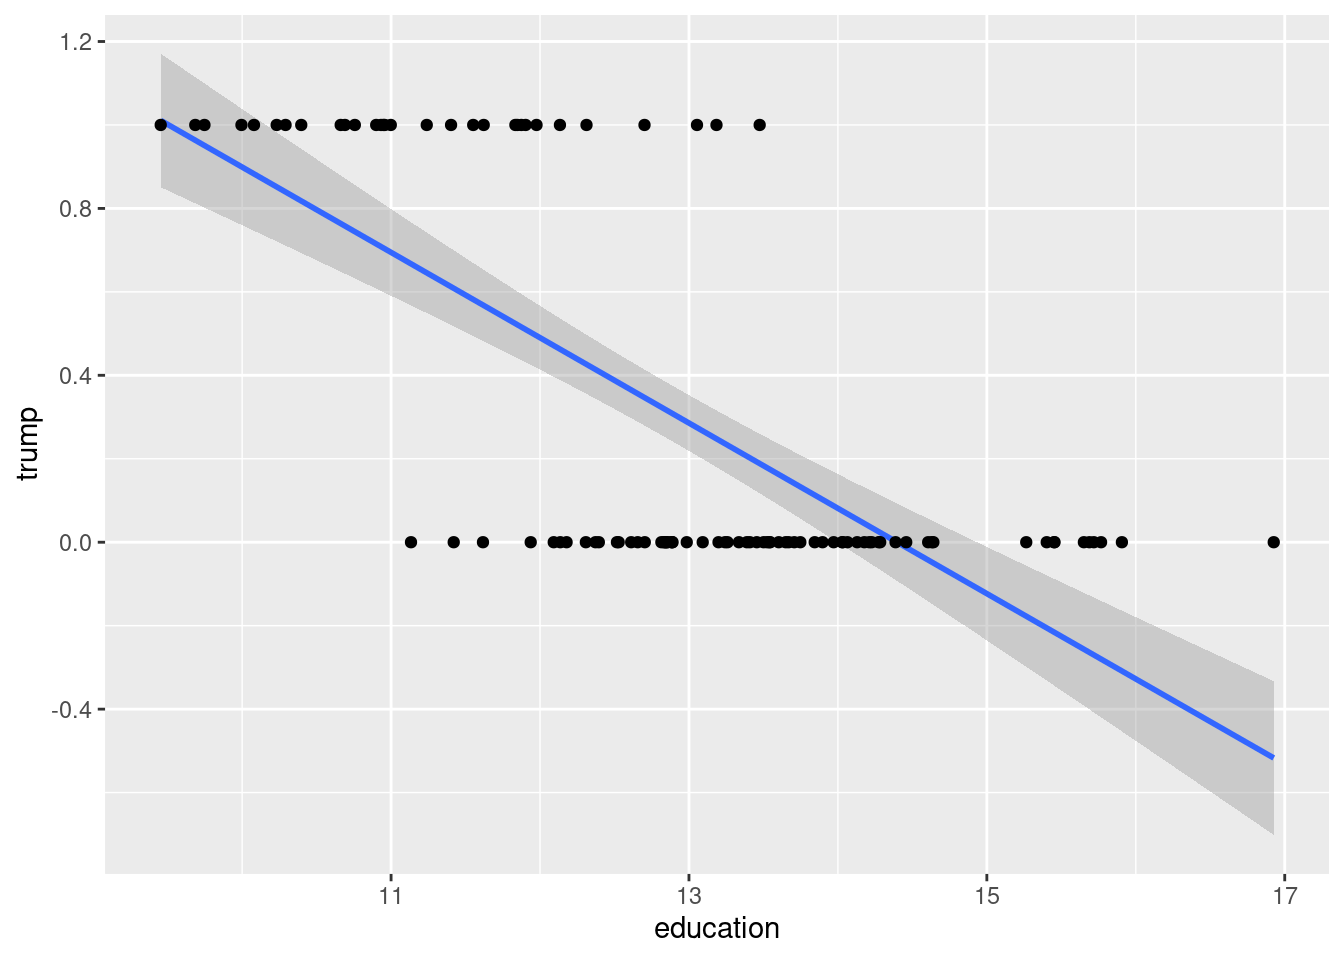
\includegraphics{pdaps_files/figure-latex/binary-scatterplot-1.pdf}

Another way to put all this is that the assumption of constant marginal effects doesn't make sense for a binary response.
If someone already has a 99\% chance of voting for Trump, the most you could possibly raise their chance of voting for him is 1\%.
This puts a cap on the magnitude of the effect of any given variable.
An intervention that raises an \emph{average} voter's chance of voting for Trump by 5\% cannot possibly have the same effect on our hypothetical Trump die-hard.
This is in contrast to settings with continuous outcomes.
A job training program that raises an average person's annual earnings by 2\% is \emph{unlikely} to have the same effect on Jeff Bezos, but it is at least \emph{conceivable} it would do so.

The idea behind logistic regression (and its close friend probit regression) is to model the conditional expectation in a way that gets around these issues.
These models always produce sensible predicted probabilities, and they assume lower-magnitude marginal effects for observations at the extremes.
Instead of regression lines, they draw nice curves like the one below.

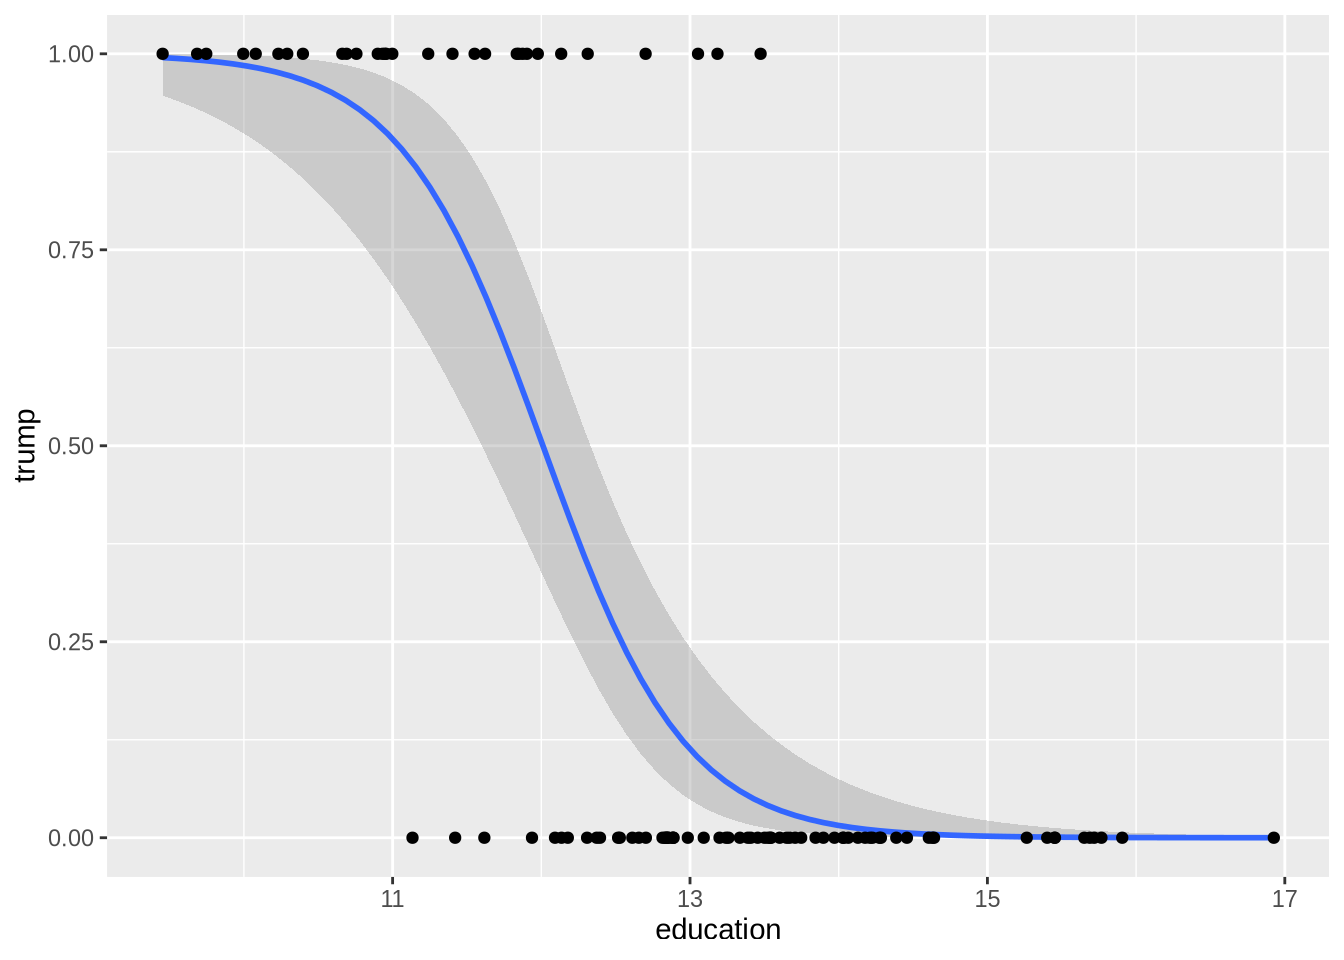
\includegraphics{pdaps_files/figure-latex/binary-scatterplot-redux-1.pdf}

\hypertarget{the-logistic-regression-model}{%
\section{The Logistic Regression Model}\label{the-logistic-regression-model}}

For a binary response, \(Y_n \in \{0, 1\}\), we can think of the linear probability model as the following:
\[
\Pr(Y_n = 1) = \mathbf{x}_n \cdot \beta.
\]
Logistic regression replaces the linear formula on the right-hand side with a nonlinear S-curve, as illustrated above.
The logistic regression model is
\[
\Pr(Y_n = 1) = \frac{e^{\mathbf{x}_n \cdot \beta}}{1 + e^{\mathbf{x}_n \cdot \beta}} = \Lambda(\mathbf{x}_n \cdot \beta),
\]
where \(\Lambda(z) = e^z / (1 + e^z)\).

How did we get the above formula?
We can tell a little story to provide a foundation for the logistic regression model.
For each observation \(n = 1, \ldots, N\), let \(Y_n^*\) denote the \emph{latent} (unobservable) propensity to choose \(Y_n = 1\).
We assume that the latent propensity follows a linear model,
\[
Y_n^* = \mathbf{x}_n \cdot \beta + \epsilon_n,
\]
where \(\epsilon_n\) is independent and identically distributed across observations.
Furthermore, assume \(\epsilon_n\) has a logistic distribution, so that \(\Pr(\epsilon_n < z) = \Lambda(z)\) for all real numbers \(z\).
Finally, we assume that we observe \(Y_n = 1\) if and only if the latent propensity is non-negative:
\[
Y_n = \begin{cases}
0 & Y_n^* < 0, \\
1 & Y_n^* \geq 0.
\end{cases}
\]
The logistic regression model follows from this combination of assumptions.

I hope you notice that the assumptions we've made on the latent propensity \(Y_n^*\) are even stronger than the usual linear model assumptions.
We assumed that \(\epsilon_n\) was independent across observations, whereas the usual linear model allows for autocorrelation.
We assumed that \(\epsilon_n\) was identically distributed across observations, whereas the usual linear model allows for heteroskedasticity.\footnote{The differences actually go even further than allowing for heteroskedasticity. We can have a homoskedastic linear model where the error variances are the same but their full distributions are different. For example, in the usual linear model we could have \(\epsilon_1 \sim U[0, 1]\) and \(\epsilon_2 \sim N(0, 1/12)\), so that \(V[\epsilon_1] = V[\epsilon_2] = 1/12\) even though their distributions differ.}
Finally, we assumed that \(\epsilon_n\) has a logistic distribution, whereas the usual linear model does not assume a specific distributional form for the error term.
The verisimilitude of the S-curve comes at the cost of forcing us to make many more assumptions than we do with a linear model.

Probit regression is the same as logistic regression, except we assume that the error term \(\epsilon_n\) in the latent propensity equation has a standard normal distribution.
This results in the model
\[
\Pr(Y_n = 1) = \Phi(\mathbf{x}_n \cdot \beta),
\]
where \(\Phi\) is the standard normal CDF.
In practice, logit and probit almost always yield nearly identical results in terms of predicted probabilities and marginal effects.
From here on we will keep working with the logistic model, solely because the logistic CDF is easier to work with mathematically than the normal CDF.

One of the nice things about the linear probability model is that it's easy to calculate marginal effects.
The estimated marginal effect of \(x_{nk}\) on \(\Pr(Y_n = 1)\) is simply its coefficient, \(\beta_k\).
It is not so simple with logistic regression.
First we need the derivative of the logistic CDF.
Surely you remember the quotient rule, which gives us
\[
\Lambda'(z)
= \frac{e^z (1 + e^z) - e^z (e^z)}{(1 + e^z)^2}
= \frac{e^z}{1 + e^z} \times \frac{1}{1 + e^z}
= \Lambda(z) [1 - \Lambda(z)].
\]
And since you surely also remember the chain rule, you can calculate the marginal effect of \(x_{nk}\) on \(\Pr(Y_n = 1)\) as
\[
\begin{aligned}
\frac{\partial \Pr(Y_n = 1)}{x_{nk}}
&= \Lambda'(\mathbf{x}_k \cdot \beta) \frac{\partial [\mathbf{x}_k \cdot \beta]}{x_{nk}} \\
&= \Lambda(\mathbf{x}_k \cdot \beta) [1 - \Lambda(\mathbf{x}_k \cdot \beta)] \beta_k \\
&= \Pr(Y_n = 1) \Pr(Y_n = 0) \beta_k.
\end{aligned}
\]
This gives us the properties we wanted---that the marginal effect of a variable is lowest in magnitude for those observations that are already highly likely or highly unlikely to have \(Y_n = 1\).

\begin{itemize}
\item
  If \(\Pr(Y_n = 1) \approx 0\), then the marginal effect of \(x_{nk}\) is approximately zero.
\item
  If \(\Pr(Y_n = 1) = 0.5\), then the marginal effect of \(x_{nk}\) is \(\beta_k / 4\).
\item
  If \(\Pr(Y_n = 1) \approx 1\), then the marginal effect of \(x_{nk}\) is approximately zero.
\end{itemize}

This gives us a helpful rule for making sense of logistic regression output.
You can divide each coefficient by 4, and that gives you its marginal effect on an observation that's at the 50-50 point.

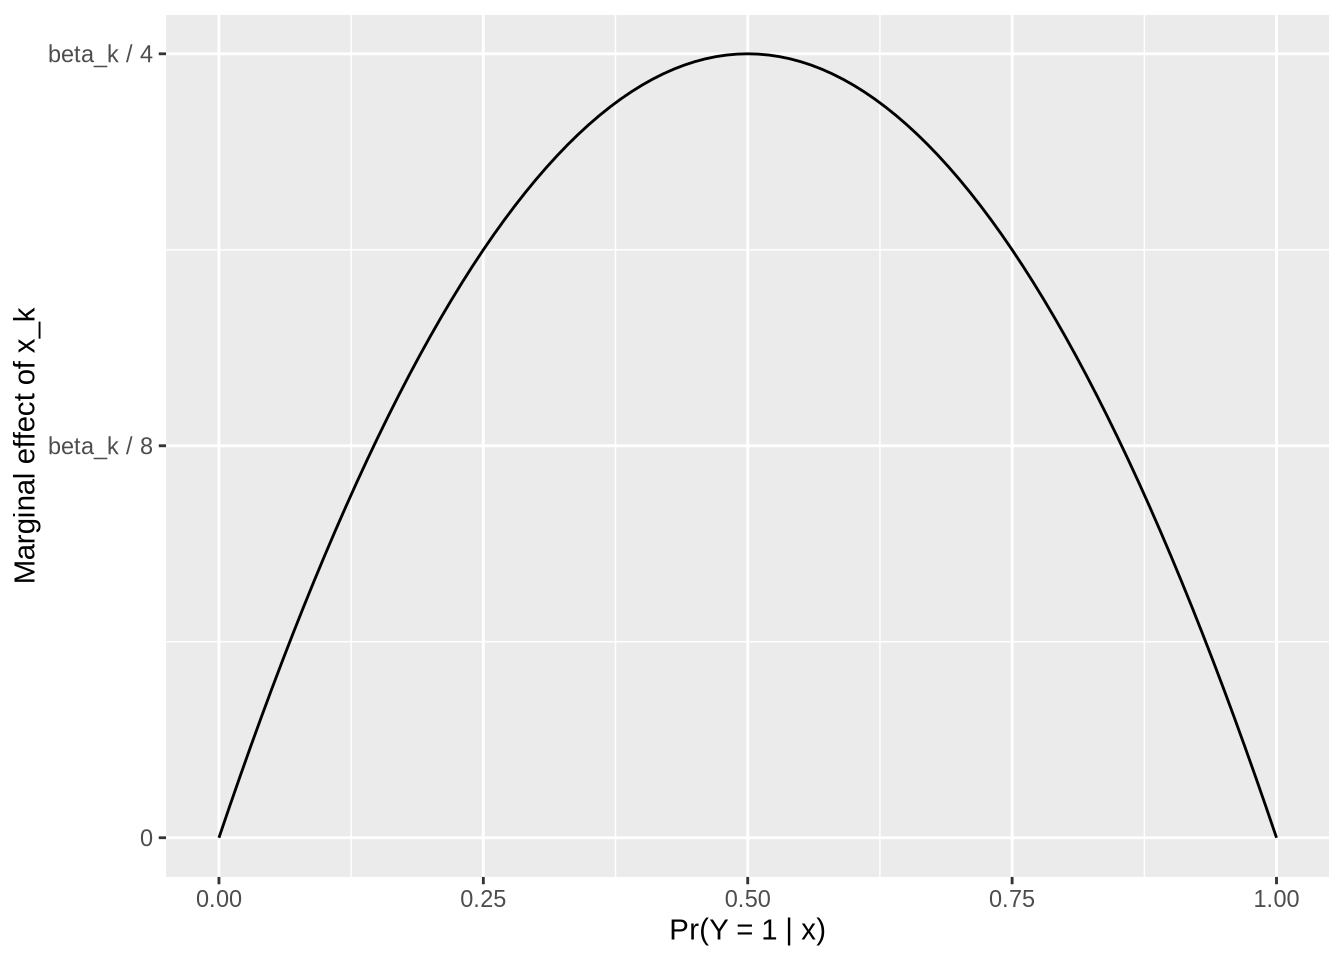
\includegraphics{pdaps_files/figure-latex/logit-margeff-1.pdf}

Briefly --- for a probit model, the marginal effect is
\[
\frac{\partial \Pr(Y_n = 1)}{x_{nk}} = \phi(\mathbf{x}_n \cdot \beta) \beta_k,
\]
where \(\phi\) is the standard normal PDF.
Since \(\phi(0) \approx 0.4\), the marginal effect for an observation at the 50-50 point is roughly 0.4 times its coefficient.

For either logit or probit, if you want to calculate the average marginal effect of \(X_k\) across your dataset, you may be tempted to calculate the marginal effect for an ``average'' observation---one with mean or median values for all the covariates.
Resist the temptation.
In both cases, the marginal effect is a nonlinear function of \(x_{nk}\), and a not-so-fun fact about nonlinear functions is that \(E[f(z)] \neq f(E[z])\).
If you want the average marginal effect, you need to calculate it individually for each observation and then average them:
\[
\text{average m.e. of $X_k$}
= \frac{\beta_k}{N} \sum_{i=1}^N \Lambda(\mathbf{x}_n \cdot \beta) [1 - \Lambda(\mathbf{x}_n \cdot \beta)]
\]

For binary covariates, we will usually focus on the first difference rather than the marginal effect, as it doesn't make much sense to take a derivative with respect to a dichotomous indicator.
Assuming \(X_k\) is binary, the first difference for the \(n\)'th observation is
\[
\Pr(Y_n = 1) - \Pr(Y_n = 0) =
\Lambda(\tilde{\mathbf{x}}_n \cdot \tilde{\beta} + \beta_k)
- \Lambda(\tilde{\mathbf{x}}_n \cdot \tilde{\beta}),
\]
where \(\tilde{\mathbf{x}}_n\) is the vector of all covariates but the \(k\)'th, and \(\tilde{\beta}\) is the vector of all coefficients but the \(k\)'th.
As with marginal effects, to calculate the average first difference across the data, you must calculate it for each observation individually and then average them---no shortcuts.

\hypertarget{maximum-likelihood-estimation}{%
\section{Maximum Likelihood Estimation}\label{maximum-likelihood-estimation}}

Remember how we derived the ordinary least squares estimator for the linear model: we decided our goal was to minimize the sum of squared residuals, then we found the formula (the function of \(\mathbf{X}\) and \(\mathbf{Y}\)) that accomplished this task.
Even though we started with a geometrical purpose (minimizing squared errors), we saw that the resulting estimator had various good statistical properties, such as unbiasedness, consistency, and asymptotic normality.

We typically don't use least squares estimators for nonlinear models like logistic regression.\footnote{You \emph{can} estimate these models with least squares, such as via the nonlinear least functions \texttt{ns()} in R. However, nonlinear least squares is inefficient relative to maximum likelihood estimation, and is usually no simpler to undertake computationally.}
Instead, we typically use \emph{maximum likelihood estimation}.
We won't go into the deeper mathematical details behind maximum likelihood estimation; for that I recommend \citet{davidson1993estimation}.

What is important to know generally about maximum likelihood estimation, or MLE, is the following:

\begin{itemize}
\item
  To derive a maximum likelihood estimator, you must specify a \emph{full probability model} for the process that generates your data.
  This entails specifying distributional families for all random variables.

  What this means is most easily illustrated by contrast with the ordinary linear model.
  With the linear model, when we wrote \(Y_n = \mathbf{x}_n \cdot \beta + \epsilon_n\), all we assumed about \(\epsilon_n\) was that it satisfied strict exogeneity and (sometimes) spherical errors.
  We didn't assume it had a normal (or any other) distribution when we derived the OLS and GLS estimators.
  But if we wanted to estimate the linear model via maximum likelihood, we would have to specify a distribution for the error term.\footnote{As it turns out, the OLS formula \emph{is} the maximum likelihood estimator for the linear model if we assume \(\epsilon_n\) is independent across observations and that each \(\epsilon_n \sim N(0, \sigma^2)\).}
\item
  The general idea behind maximum likelihood estimation is to find the model parameters under which our observed data is most likely to have occurred.
  If you draw a random sample of Democratic primary voters, and 68\% of them tell you that they prefer Joe Biden over Bernie Sanders, it is \emph{possible} that in fact Biden's support in the population is 10\%, or that it's 90\%.
  However, we'd be much more likely to draw the sample that we did if the true population proportion is 68\% than if it were 10\% or 90\%.
  We will rely on this kind of reasoning to develop maximum likelihood estimators.
\item
  As long as your model of the data-generating process is correctly specified, the maximum likelihood estimator is \emph{consistent}, \emph{asymptotically normal}, and \emph{asymptotically efficient}.
  This means that in sufficiently large samples:

  \begin{itemize}
  \item
    The maximum likelihood estimate from any given sample is likely to be close to the population parameter value.
  \item
    The distribution of maximum likelihood estimates across samples is approximately normal.
  \item
    No other consistent estimator will have smaller standard errors.
  \end{itemize}
\end{itemize}

Maximum likelihood estimation is built around the \emph{likelihood function}.
Let \(\mathbf{Z}\) denote the data we observe, and let \(\theta\) denote the parameters we want to estimate.
In the regression context, \(\mathbf{Z}\) would consist of the response \(\mathbf{Y}\) and the covariates \(\mathbf{X}\), and \(\theta\) would consist of the coefficients \(\beta\).
The likelihood function, which I'll denote \(\ell(\theta, \mathbf{Z})\), is the probability that we would observe the given data, \(\mathbf{Z}\), if the parameters of the model were \(\theta\).
The maximum likelihood estimator is the value of \(\theta\) at which \(\ell\) reaches its maximum, given the data \(\mathbf{Z}\); it is the parameter value under which we have the highest chance of observing our actual data.
In case this sounds either trivial or incomprehensible, let's make it concrete by working through some simple examples.

\hypertarget{properties-of-logarithms}{%
\subsection{Properties of logarithms}\label{properties-of-logarithms}}

As you'll see below, we often run into the natural logarithm in maximum likelihood estimation.
So let's briefly refresh ourselves on the most important properties of the natural logarithm.

Remember that the natural logarithm is the inverse of the natural exponent.
For all \(s \in \mathbb{R}\) and \(t > 0\),
\[
\log (t) = s \quad \Leftrightarrow \quad e^s = t,
\]
where \(e\) is Euler's number, \(e \approx 2.71828\).
Exponents and logarithms have some helpful properties that will become second nature once you work with them enough.

\begin{longtable}[]{@{}ll@{}}
\toprule
Exponent Property & Logarithm Property\tabularnewline
\midrule
\endhead
\(e^{a + b} = e^a \cdot e^b\) & \(\log (ab) = \log(a) + \log(b)\)\tabularnewline
\(e^{a - b} = \frac{e^a}{e^b}\) & \(\log (\frac{a}{b}) = \log(a) - \log(b)\)\tabularnewline
\(e^{ab} = (e^a)^b\) & \(\log (a^b) = b \log (a)\)\tabularnewline
\bottomrule
\end{longtable}

The natural logarithm plays a special role in differential calculus as well.
Remember the power rule,
\[
\frac{d x^n}{d x} = n x^{n-1}.
\]
If we apply the power rule in reverse, we see that
\[
\begin{aligned}
\frac{d}{dx} \left[ \frac{x^3}{3} \right] &= x^2, \\
\frac{d}{dx} \left[ \frac{x^2}{2} \right] &= x^1, \\
\frac{d}{dx} \left[ \frac{x^1}{1} \right] &= x^0 (= 1) \\
\frac{d}{dx} \left[ \text{???} \vphantom{\frac{x^0}{0}} \right] &= x^{-1} (= \frac{1}{x}) \\
\frac{d}{dx} \left[ \frac{x^{-1}}{-1} \right] &= x^{-2} (= \frac{1}{x^2}).
\end{aligned}
\]
If we tried to fill in according to the pattern to find the function whose derivative is \(x^{-1}\), we would end up with \(\frac{x^0}{0}\), better known as \(\frac{1}{0}\), which can't possibly be right.
It turns out instead that the natural logarithm plays this role:
\[
\frac{d \log(x)}{dx} = \frac{1}{x}.
\]

We will often encounter expressions of the form \(\log(f(x))\), where \(f(x)\) is some differentiable function of \(x\).
In this case, applying the chain rule, we have
\[
\frac{d \log(f(x))}{dx} = \frac{\frac{d f(x)}{dx}}{f(x)}.
\]
This is another one of those operations that will become second nature over time.

\hypertarget{bernoulli-trials}{%
\subsection{Bernoulli trials}\label{bernoulli-trials}}

Assume we observe a sequence of independent random variables \(Z_1, \ldots, Z_N\), where each \(Z_n \sim \text{Bernoulli}(p)\).
Our goal is to estimate \(p\), the population probability of a ``success'' \(Z_n = 1\) as opposed to a ``failure'' \(Z_n = 0\).

Suppose we only had a single observation, \(N = 1\).
What would the likelihood function, \(\ell(p, Z_1)\), look like?
Well, there are two possible samples: \(Z_1 = 0\) or \(Z_1 = 1\).
If the population parameter is \(p\) and our observed sample is \(Z_1 = 0\), the probability of observing this sample is \(1 - p\).
Conversely, if our observed sample is \(Z_1 = 1\), the probability of observing this sample is \(p\).
Hence, the likelihood function is
\[
\ell(p, Z_1) = \begin{cases}
1 - p & Z_1 = 0, \\
p & Z_1 = 1.
\end{cases}
\]
Now let's think about choosing \(p\) to \emph{maximize} the likelihood function.
If \(Z_1 = 0\), then the likelihood function is strictly decreasing in \(p\), so we want to choose the smallest value possible: \(p = 0\).
If \(Z_1 = 1\), we are have the opposite: the likelihood function is strictly increasing in \(p\), and thus is maximized at \(p = 1\).
Altogether, we have the maximum likelihood estimator:
\[
\hat{p}_{\text{MLE}}(Z_1) = \begin{cases}
0 & Z_1 = 0, \\
1 & Z_1 = 1,
\end{cases}
\]
or, more simply, \(\hat{p}_{\text{MLE}}(Z_1) = Z_1\).

Now let's think about the more general case, where \(\mathbf{Z} = (Z_1, \ldots, Z_N)\).
Since each observation is independent, the likelihood function is multiplicative:
\[
\ell(p, \mathbf{Z})
= \Pr(Z = Z_1) \times \Pr(Z = Z_2) \times \cdots \times \Pr(Z = Z_N)
= \prod_{n=1}^N \Pr(Z = Z_n).
\]
For those observations where \(Z_n = 0\), the probability of observing this outcome is \(1 - p\).
For those where \(Z_n = 1\), the probability is \(p\).
So we can further write
\[
\ell(p, \mathbf{Z})
= \prod_{n : Y_N = 0} (1 - p) \prod_{n : Y_N = 1} p
= (1 - p)^{N - N_1} p^{N_1},
\]
where \(N_1\) is the number of successes, \(N_1 = \sum_{n=1}^N Y_n\).

We want to maximize \(\ell\) with respect to \(p\).
That is, we want to find the value \(\hat{p}\) such that
\[
\ell(\hat{p}, \mathbf{Z}) \geq \ell(p, \mathbf{Z}) \qquad \text{for all $p \in [0, 1]$.}
\]
This is a maximization problem.
We solve maximization problems the same way we solved the minimization problem of OLS---by finding the point at which the derivative equals zero.
Here, we want to find the point at which the derivative of the likelihood function with respect to \(p\) equals zero.

Taking derivatives of products is annoying.
It's way easier to take derivatives of sums, because the derivative of the sum is the sum of the derivatives.
Therefore, likelihood-based statistical methods usually work with the \emph{log-likelihood}, the natural logarithm of the likelihood function.
Because the logarithm is a strictly increasing function, it is maximized at the same point as the likelihood function.
Consequently, we will look for the value \(\hat{p}\) such that
\[
\log \ell(\hat{p}, \mathbf{Z}) \geq \log \ell(p, \mathbf{Z}) \qquad \text{for all $p \in [0, 1]$},
\]
which we will find by solving for \(\hat{p}\) in
\[
\frac{\partial \log \ell(\hat{p}, \mathbf{Z})}{\partial p} = 0.
\]

For the Bernoulli problem, we have
\[
\begin{aligned}
\log \ell(p, \mathbf{Z}) &= \log \left[ (1 - p)^{N - N_1} p^{N_1} \right] \\
&= (N - N_1) \log(1 - p) + N_1 \log(p)
\end{aligned}
\]
and therefore
\[
\begin{aligned}
\frac{\partial \log \ell(p, \mathbf{Z})}{\partial p}
&= \frac{-(N - N_1)}{1 - p} + \frac{N_1}{p}.
\end{aligned}
\]
We solve for the maximum likelihood estimate by setting the above expression to equal zero, giving us the condition
\[
\begin{aligned}
\frac{N_1}{\hat{p}} = \frac{N - N_1}{1 - \hat{p}}.
&\quad\Leftrightarrow\quad N_1 - N_1 \hat{p} = N \hat{p} - N_1 \hat{p} \\
&\quad\Leftrightarrow\quad \hat{p} = \frac{N_1}{N}.
\end{aligned}
\]
Finally, therefore, the maximum likelihood estimator is the sample proportion of successes,
\[
\hat{p}_{\text{MLE}}(\mathbf{Z}) = \frac{\sum_{n=1}^N Z_n}{N}.
\]

All that seems like a \emph{lot} of effort to come to the conclusion that we should estimate the parameter of the Bernoulli distribution via the sample proportion of successes.
Didn't we already know that?
Yes, we did, but this is a relatively easy example for working through the mechanics of deriving a maximum likelihood estimator.
Additionally, we'll return to the Bernoulli example once we develop the maximum likelihood estimator for binary response models.
Now, we'll turn to a less trivial example, where the maximum likelihood estimator will differ from what other estimation approaches would tell us to do.

\hypertarget{uniform-draws}{%
\subsection{Uniform draws}\label{uniform-draws}}

Assume we observe a sequence of independent random variables \(Z_1, \ldots, Z_N\), where each \(Z_n \sim U[0, \theta]\).
Our goal is to estimate \(\theta\), the upper bound of the support of this uniform distribution.
Remember that the probability density function of \(U[0, \theta]\) is
\[
f_\theta(z) = \begin{cases}
0 & z < 0, \\
\frac{1}{\theta} & 0 \leq z \leq \theta, \\
0 & z > \theta.
\end{cases}
\]

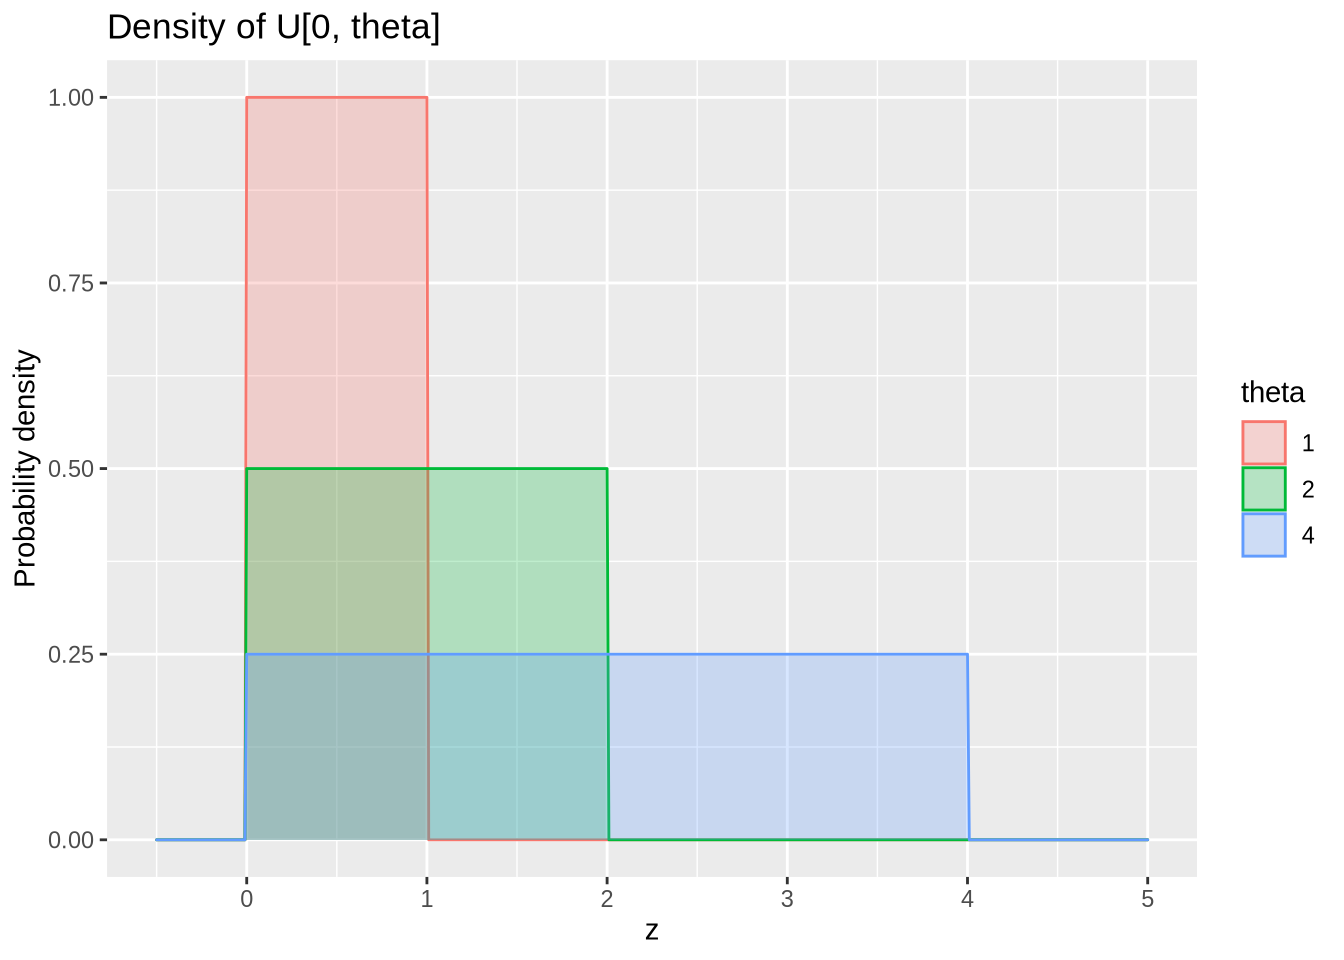
\includegraphics{pdaps_files/figure-latex/uniform-dens-1.pdf}

There is a simple unbiased estimator of \(\theta\) available to us.
Let \(\bar{Z}\) denote our sample mean, \(\bar{Z} = \frac{1}{N} \sum_{n=1}^N Z_n\).
Then \(\hat{\theta}_{\text{MM}}(\mathbf{Z}) = 2 \bar{Z}\) is an unbiased estimator of \(\theta\).\footnote{The ``MM'' subscript denotes the fact that \(\hat{\theta}_{\text{MM}}\) is a \emph{method of moments} estimator of \(\theta\). Like maximum likelihood estimation, the method of moments is a set of principles used to derive estimators.}
This is true because (1) the population mean of \(U[0, \theta]\) is \(\frac{\theta}{2}\) and (2) the sample mean is an unbiased estimator of the population mean, and thus we have
\[
E[\hat{\theta}_{\text{MM}}(\mathbf{Z})]
= E[2 \bar{Z}]
= 2 E[\bar{Z}]
= \theta.
\]

Here we see why an unbiased estimator is not always best.
Suppose we observe the following data with \(N = 3\):
\[
Z_1 = 1, \quad Z_2 = 2, \quad Z_3 = 9.
\]
We have the sample mean \(\bar{Z} = 4\), so our unbiased estimate of the population parameter \(\theta\) is \(\hat{\theta}_{\text{MM}}(\mathbf{Z}) = 8\).
But this is crazy, because this data cannot possibly have been drawn from \(U[0, 8]\)!
If this were the true distribution, then it would be impossible to observe \(Z_3 = 9\).

Let's see how we would estimate \(\theta\) via maximum likelihood.
This time our data is continuous, so the likelihood function gives us the density of the data given the parameters:
\[
\begin{aligned}
\ell(\theta, \mathbf{Z})
&= f_\theta(Z_1) \times f_\theta(Z_2) \times \cdots \times f_\theta(Z_n) \\
&= \prod_{n=1}^N f_\theta(Z_n).
\end{aligned}
\]
Substituting in the definition of the \(U[0, \theta]\) density from above, we have
\[
\ell(\theta, \mathbf{Z}) = \begin{cases}
0 & \text{any $Z_n < 0$ or $Z_n > \theta$}, \\
\frac{1}{\theta^N} & \text{all $0 \leq Z_n \leq \theta$}.
\end{cases}
\]
This time, we don't even need to work with the log-likelihood or take derivatives to see that the likelihood will be maximized at \(\theta = \max \{Z_1, \ldots, Z_N\}\).
If we return to our example with \(\mathbf{Z} = (1, 2, 9)\), the likelihood function looks like this:

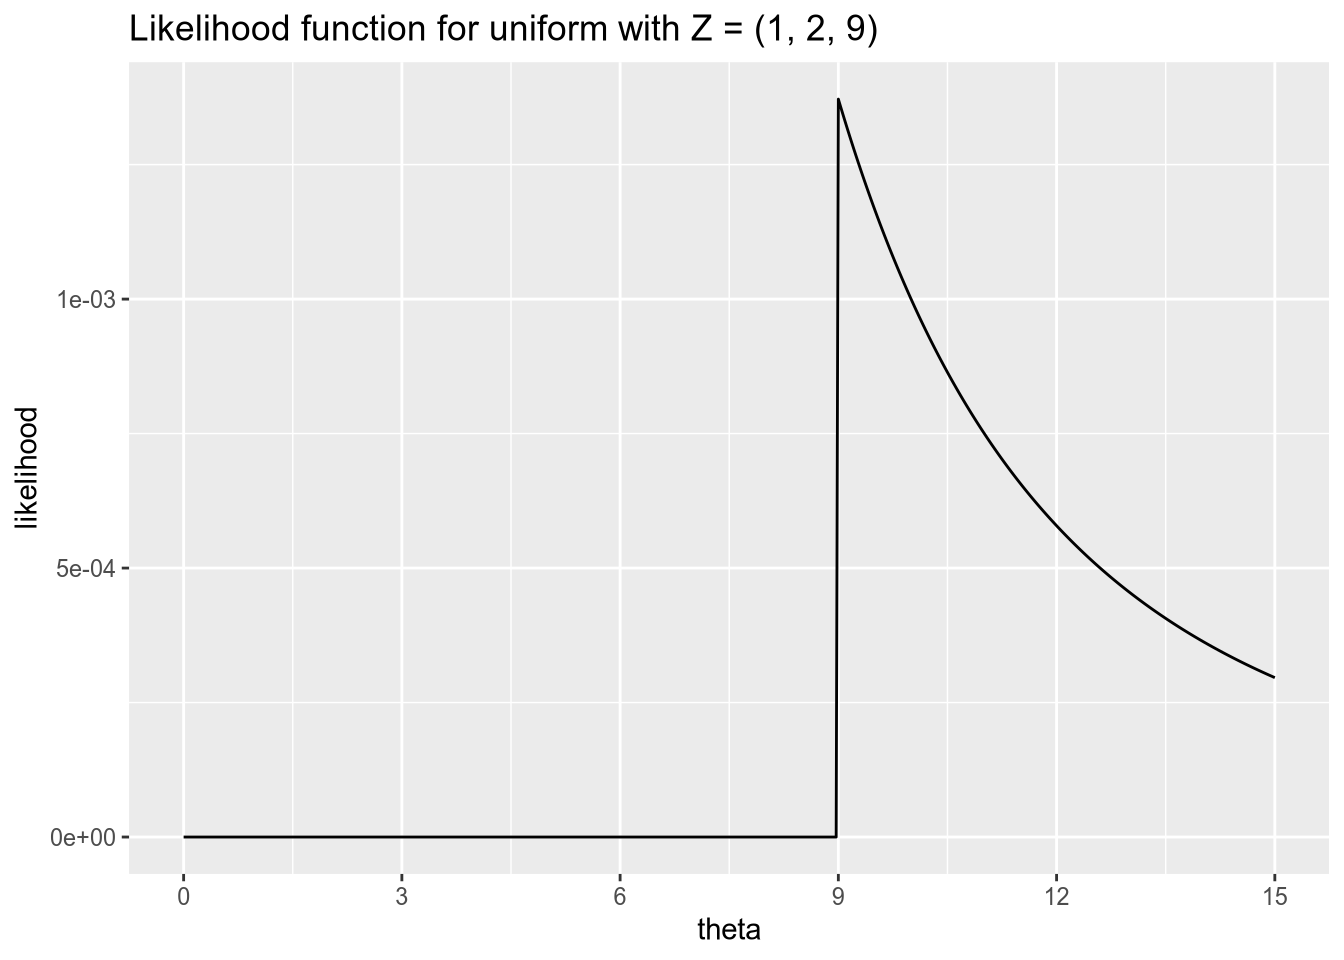
\includegraphics{pdaps_files/figure-latex/lik-unif-1.pdf}

Our maximum likelihood estimator for \(\theta\) in this model is therefore
\[
\hat{\theta}_{\text{MLE}}(\mathbf{Z}) = \max \{ Z_1, \ldots, Z_N \}.
\]
This is a biased estimator.
To see why, imagine taking numerous different samples from \(U[0, \theta]\) and calculating the MLE for each of them.
We will almost always have \(\hat{\theta}_{\text{MLE}} < \theta\), and we will never have \(\hat{\theta}_{\text{MLE}} > \theta\).
Consequently, the MLE will on average underestimate the true value of \(\theta\).
Nonetheless, the MLE has two advantages over the unbiased estimator we considered.
First, it will never yield an estimate that would be impossible given the observed data.
Second, as our sample size grows large, even though the MLE is biased, it will on average be closer to the true \(\theta\) than the unbiased estimate will be.
This is because maximum likelihood estimation is asymptotically efficient.

I want to stress one more important thing that this example highlights.
However you choose to model the data-generating process, there are multiple distinct ways to estimate the parameters of that process.
We already saw this in the linear model context, where OLS and GLS are distinct estimators of the same linear model, each of which is preferable in different circumstances.
You may sometimes hear political scientists refer to ``maximum likelihood models'', but this is a misnomer: maximum likelihood is just one method among many to estimate the parameters of a fully specified statistical model.
It happens to have quite good properties for doing so, and hence is usually the default choice, but that doesn't mean maximum likelihood is embedded in the definition of the model itself.

\hypertarget{logistic-regression}{%
\subsection{Logistic regression}\label{logistic-regression}}

Now let's return to the logistic regression model.
Here we observe a sequence of outcomes, \(Y_1, \ldots, Y_N\), where each \(Y_n \in \{0, 1\}\), and a sequence of covariate vectors, \(\mathbf{x}_1, \ldots, \mathbf{x}_N\).
Our goal is to estimate \(\beta\), the coefficients associated with each entry in \(\mathbf{x}_n\).

Remember that under the logistic regression model,
\[
\Pr(Y_n = 1 \,|\, \mathbf{x}_n)
= \frac{e^{\mathbf{x}_n \cdot \beta}}{1 + e^{\mathbf{x}_n \cdot \beta}}
= \Lambda(\mathbf{x}_n \cdot \beta).
\]
By the same token, \(\Pr(Y_n = 0 \,|\, \mathbf{x}_n) = 1 - \Lambda(\mathbf{x}_n \cdot \beta)\).
Following the same logic as in the case of a sequence of Bernoulli random variables, this means the likelihood function for the logistic regression model is a big ugly product,
\[
\ell(\beta, \mathbf{Y}, \mathbf{X})
= \prod_{n : Y_n = 0} (1 - \Lambda(\mathbf{x}_n \cdot \beta)) \prod_{n : Y_n = 1} \Lambda(\mathbf{x}_n \cdot \beta).
\]
We will make this easier to work with by taking the log-likelihood,
\[
\begin{aligned}
\log \ell(\beta, \mathbf{Y}, \mathbf{X})
&= \sum_{n : Y_n = 0} \log (1 - \Lambda(\mathbf{x}_n \cdot \beta)) + \sum_{n : Y_n = 1} \log \Lambda (\mathbf{x}_n \cdot \beta) \\
&= \sum_{n=1}^N \left[ \vphantom{\sum} (1 - Y_n) \log (1 - \Lambda(\mathbf{x}_n \cdot \beta)) + Y_n \log \Lambda (\mathbf{x}_n \cdot \beta) \right]
\end{aligned}
\]

If you followed the Bernoulli example, you can guess what comes next.
The log-likelihood is maximized at the point where its partial derivatives all equal zero, so you can't increase it further by moving in any direction.
So what we'll do now is take the \emph{gradient}, or the vector of all partial derivatives,
\[
\nabla \log \ell(\beta, \mathbf{Y}, \mathbf{X})
= \left( \frac{\partial \log \ell(\beta, \mathbf{Y}, \mathbf{X})}{\partial \beta_1}, \cdots, \frac{\partial \log \ell(\beta, \mathbf{Y}, \mathbf{X})}{\partial \beta_K} \right).
\]
Then we'll find the maximum of the log-likelihood by setting \(\nabla \log \ell(\beta, \mathbf{X}, \mathbf{Y}) = \mathbf{0}\) and solving for \(\beta\) (\(K\) equations in \(K\) unknowns).

Only there's one problem.
If you try to do that, you can't explicitly solve for \(\beta\) as a function of \(\mathbf{X}\) and \(\mathbf{Y}\).
There's no way to finagle the condition such that \(\beta\) is on one side and some function of \(\mathbf{X}\) and \(\mathbf{Y}\) are on the other side, the way we did to derive the OLS estimator.
In other words, unlike with OLS and GLS, there's no formula that gives us the logistic regression coefficients.

Then what is your statistical software doing when you run a logistic regression?
It uses an \emph{iterative} solver to come up with a best guess for the maximum likelihood estimate.
Without going too deeply into the details, here is what an iterative solver does.

\begin{enumerate}
\def\labelenumi{\arabic{enumi}.}
\item
  Start with an initial guess for \(\hat{\beta}\).
  For example, you might use the OLS coefficients.
\item
  Repeat the following process until it terminates or you run out of patience:

  \begin{enumerate}
  \def\labelenumii{\alph{enumii}.}
  \item
    Check whether \(\nabla \log \ell(\hat{\beta}, \mathbf{Y}, \mathbf{X}) \approx \mathbf{0}\). If so, terminate. Otherwise, continue.
  \item
    Update your current guess about \(\hat{\beta}\) by nudging it in the direction of quickest ascent, namely the gradient \(\nabla \log \ell(\hat{\beta}, \mathbf{Y}, \mathbf{X})\).
  \end{enumerate}
\end{enumerate}

The standard errors are then calculated using the matrix of second partial derivatives of the log-likelihood.
I will spare you the math here.
The important thing to know about the standard errors is that they are only ``correct'', in the sense of properly estimating the degree of uncertainty in your model estimates, asymptotically.
The logistic regression coefficients themselves are consistent but not unbiased, meaning they are only guaranteed to be reliable in sufficiently large samples, and the same is true of the inferential statistics.
If you find yourself in the dubious situation of running a logistic regression on a very small sample---such as because a reviewer asked you do to so in an R\&R, because surely you wouldn't do this voluntarily knowing what you know now---you should not rely on the default standard error computation when performing hypothesis tests.

\hypertarget{special-considerations}{%
\section{Special Considerations}\label{special-considerations}}

\hypertarget{separation}{%
\subsection{Separation}\label{separation}}

Sometimes you may have a covariate that perfectly predicts whether the outcome is a 0 or a 1.
For example, on many contentious votes in Congress, whether a member votes yay or nay will be determined entirely by her partisanship.
This phenomenon is called \emph{complete separation} (terminology from \citet{albert1984existence}), and it is a vexing problem for the maximum likelihood estimation of logistic regression models.

Let's imagine a dataset where we have a single covariate \(X\), the response is 0 whenever \(X\) is negative, and the response is 1 whenever \(X\) is positive.

\begin{verbatim}
## # A tibble: 6 x 2
##       y     x
##   <dbl> <int>
## 1     0    -3
## 2     0    -2
## 3     0    -1
## 4     1     1
## 5     1     2
## 6     1     3
\end{verbatim}

Now let's imagine fitting a logistic regression model to this data: \(\Pr(Y = 1 | X) = \Lambda(X \cdot \beta)\).
Because of the complete separation on \(X\), a maximum likelihood estimate does not exist.
No matter how high \(\beta\) is, we can improve the likelihood by increasing it further.
In effect, our estimate would be \(\hat{\beta} = \infty\).

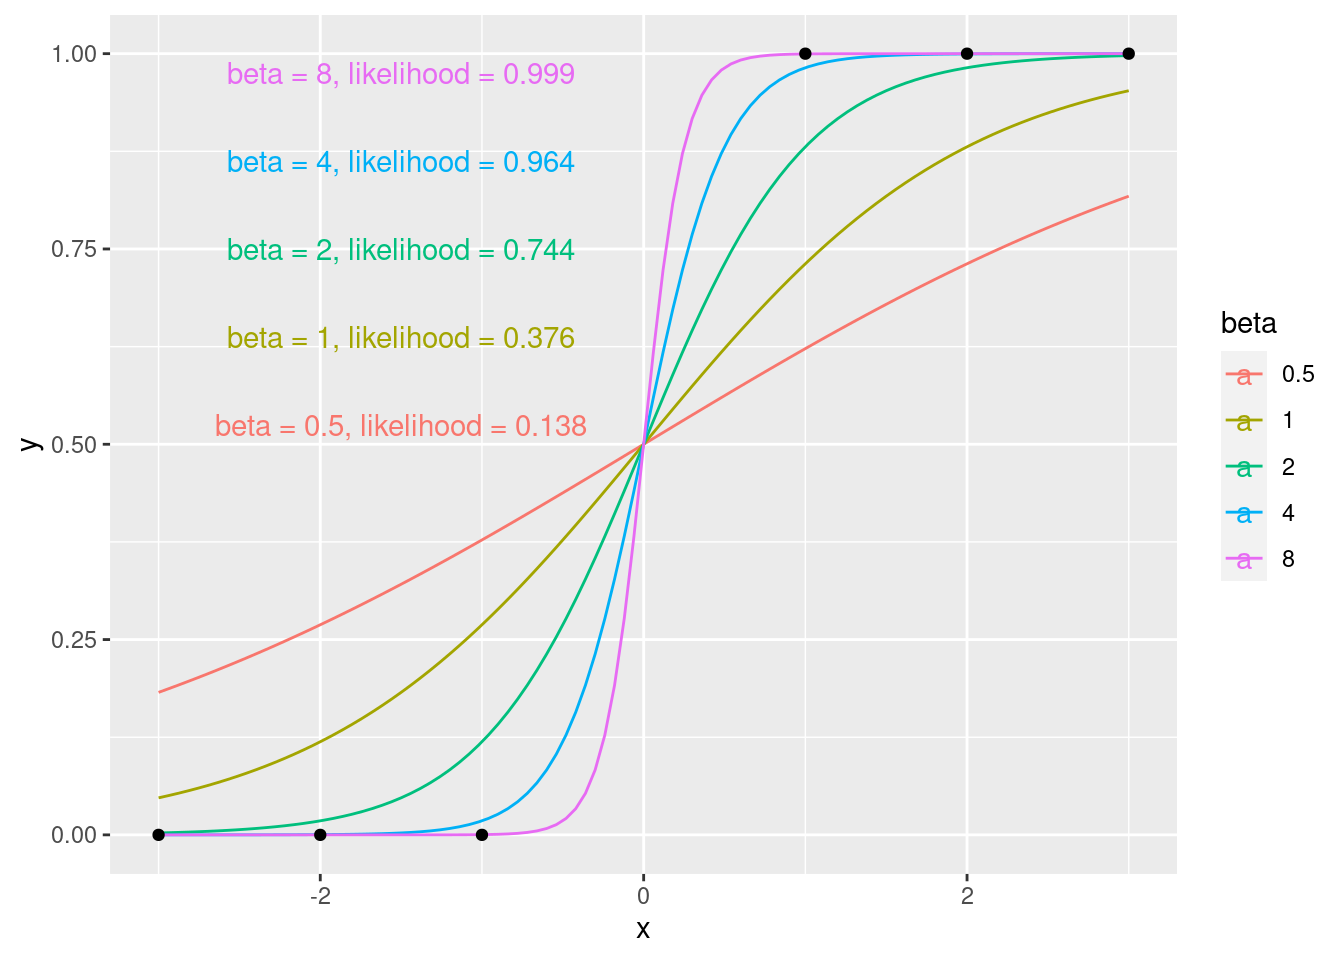
\includegraphics{pdaps_files/figure-latex/logit-sep-curves-1.pdf}

If we try to actually fit a logistic regression to this data, we get nonsensical results.

\begin{Shaded}
\begin{Highlighting}[]
\NormalTok{fit\_sep \textless{}{-}}\StringTok{ }\KeywordTok{glm}\NormalTok{(y }\OperatorTok{\textasciitilde{}}\StringTok{ }\NormalTok{x,}
               \DataTypeTok{family =} \KeywordTok{binomial}\NormalTok{(}\DataTypeTok{link =} \StringTok{"logit"}\NormalTok{),}
               \DataTypeTok{data =}\NormalTok{ separated\_data)}
\end{Highlighting}
\end{Shaded}

\begin{verbatim}
## Warning: glm.fit: fitted probabilities numerically 0 or 1 occurred
\end{verbatim}

\begin{Shaded}
\begin{Highlighting}[]
\KeywordTok{summary}\NormalTok{(fit\_sep)}
\end{Highlighting}
\end{Shaded}

\begin{verbatim}
## 
## Call:
## glm(formula = y ~ x, family = binomial(link = "logit"), data = separated_data)
## 
## Deviance Residuals: 
##          1           2           3           4           5           6  
## -2.110e-08  -2.110e-08  -1.253e-05   1.253e-05   2.110e-08   2.110e-08  
## 
## Coefficients:
##               Estimate Std. Error z value Pr(>|z|)
## (Intercept) -9.002e-08  4.842e+04       0        1
## x            2.327e+01  4.842e+04       0        1
## 
## (Dispersion parameter for binomial family taken to be 1)
## 
##     Null deviance: 8.3178e+00  on 5  degrees of freedom
## Residual deviance: 3.1384e-10  on 4  degrees of freedom
## AIC: 4
## 
## Number of Fisher Scoring iterations: 24
\end{verbatim}

The warning ``fitted probabilities numerically 0 or 1 occurred'' is R's way of letting us know that there was complete separation, so the logistic regression results should not be trusted.

A closely related but slightly less serious problem is \emph{quasicomplete separation}.
Remember that complete separation is a perfect correlation between the covariate and the response: once I know \(X_n\), then I am sure about the corresponding \(Y_n\), and vice versa.
Quasicomplete separation is when this holds partially, so that some values of \(X_n\) perfectly predict \(Y_n\) but others do not.

Quasicomplete separation is best illustrated by example.
In 2010, the Affordable Care Act passed the House by a 219-212 vote.
Every Republican in the House voted against the bill, whereas Democrats were split 219-34.
This means we would have quasicomplete separation in a logistic regression of ACA vote on partisanship.
Once I know a member is a Republican, I would be certain they voted against.
However, knowing a member is a Democrat does not by itself predict if they voted for or against the bill.
So if I included an indicator for being a Republican in the model, its maximum likelihood estimate would not exist, as the likelihood would always improve as the coefficient approached \(- \infty\).
However, I could use the variation among the Democratic members to estimate the effects of other variables, such as President Obama's vote share in the members' districts.

It is an open question what to do in the presence of complete or quasicomplete separation.
Sometimes separation is an indication that you're asking a question that the data can't reasonably answer.
Alternatively, \citet{zorn2005solution} recommends using the bias-corrected logistic regression estimator developed by \citet{firth1993bias}.
What you should \emph{not} do is report whatever numbers your statistical software spits out as if they were proper maximum likelihood estimates --- they are not.
It is also usually a bad idea to simply remove the offending variable from your analysis, unless this variable is uncorrelated with your treatment of interest (in which case, why was it in your analysis to begin with?).

\hypertarget{fixed-effects-1}{%
\subsection{Fixed Effects}\label{fixed-effects-1}}

There are a couple of issues with the use of fixed effects in logistic regression models.
The first is that fixed effects are often a source of quasicomplete separation.
For example, imagine that you have data on individuals grouped within households, and your response variable is whether each individual voted in the most recent election.
You will have quasicomplete separation on the indicator for any household where every member voted or where no member voted.

A second, more subtle problem concerns the consistency of fixed effects estimators for the logistic regression model.
I said before that maximum likelihood estimators are guaranteed to be consistent.
This is true when the number of parameters of the model is fixed even as the sample size grows.
However, this is not necessarily true in the case of fixed effects.
Again, imagine our example of individuals grouped within households.
Collecting more data means surveying more households, which means including more household fixed effects in your regression model.
The number of parameters to estimate grows with the sample size.
Consequently, the maximum likelihood estimator is not consistent.
This is an example of the \emph{incidental parameters problem}.

The usual fix for the incidental parameters problem is to use the ``conditional logit'' estimator developed by \citet{chamberlain1980analysis}.
Very loosely speaking, this is an alternative estimation approach that estimates the coefficients on the substantive parameters by examining only within-group variation.
Another method is to simply use a linear probability model, in which fixed effects estimation is less problematic.
\citet{beck2018estimating} compares these approaches.

\hypertarget{autocorrelation-and-clustered-standard-errors}{%
\subsection{Autocorrelation and Clustered Standard Errors}\label{autocorrelation-and-clustered-standard-errors}}

We constructed the likelihood function for logistic regression under the assumption of independent and identically distributed observations.
If there is correlation in the random noise across observations, then our likelihood function is wrong.
Specifically, if there is autocorrelation between observations \(m\) and \(n\), then we have
\[
\Pr(Y_m = a, Y_n = b \,|\, \mathbf{x}_m, \mathbf{x}_n)
\neq \Pr(Y_m = a \,|\, \mathbf{x}_m) \Pr(Y_n = b \,|\, \mathbf{x}_n).
\]
But we wrote out the likelihood function under the assumption that we could take the product this way.
So if you suspect that you have autocorrelation and yet you run an ordinary logistic regression, you are not doing maximum likelihood estimation (because your likelihood function is wrong), and you cannot rely on its good properties like consistency anymore.

There are special estimators tailored for binary response models with autocorrelation.
These are typically complicated to estimate and interpret, and so they are well beyond the scope of this course.
See \citet{huffer1998markov} or, for an introduction aimed at political scientists, \citet{ward2002location}.
Alternatively, you may prefer to just use a linear probability model.

Should you decide to go ahead and use the nominal logistic regression estimator even though it's not actually MLE in the presence of autocorrelation, there are software packages that will provide clustered standard error estimates.
These follow the same kind of ``sandwich'' logic as the formula we derived for OLS \citep{Liang:1986gv}.
In some cases the ordinary estimator may still be consistent, though it will not be efficient.
This requires, very loosely speaking, that the average autocorrelation between observations go to zero as the sample size increases \citep{poirier1988probit}.\footnote{I thank Larry Bartels for drawing my attention to the reference here, in response to a question by a previous PSCI 8357 student.}

\hypertarget{appendix-implementation-in-r-2}{%
\section{Appendix: Implementation in R}\label{appendix-implementation-in-r-2}}

\hypertarget{logistic-regression-1}{%
\subsection{Logistic Regression}\label{logistic-regression-1}}

To illustrate logistic regression in R, we will use data from the \textbf{pscl} package on how senators voted on the 2002 resolution to authorize military force against Iraq.

\begin{Shaded}
\begin{Highlighting}[]
\KeywordTok{library}\NormalTok{(}\StringTok{"pscl"}\NormalTok{)}
\KeywordTok{head}\NormalTok{(iraqVote)}
\end{Highlighting}
\end{Shaded}

\begin{verbatim}
##   y state.abb             name  rep state.name gorevote
## 1 1        AL  SESSIONS (R AL) TRUE    Alabama    41.59
## 2 1        AL    SHELBY (R AL) TRUE    Alabama    41.59
## 3 1        AK MURKOWSKI (R AK) TRUE     Alaska    27.67
## 4 1        AK   STEVENS (R AK) TRUE     Alaska    27.67
## 5 1        AZ       KYL (R AZ) TRUE    Arizona    44.67
## 6 1        AZ    MCCAIN (R AZ) TRUE    Arizona    44.67
\end{verbatim}

\begin{Shaded}
\begin{Highlighting}[]
\KeywordTok{summary}\NormalTok{(iraqVote)}
\end{Highlighting}
\end{Shaded}

\begin{verbatim}
##        y          state.abb              name       rep         
##  Min.   :0.00   AK     : 2   AKAKA (D HI)  : 1   Mode :logical  
##  1st Qu.:1.00   AL     : 2   ALLARD (R CO) : 1   FALSE:51       
##  Median :1.00   AR     : 2   ALLEN (R VA)  : 1   TRUE :49       
##  Mean   :0.77   AZ     : 2   BAUCUS (D MT) : 1                  
##  3rd Qu.:1.00   CA     : 2   BAYH (D IN)   : 1                  
##  Max.   :1.00   CO     : 2   BENNETT (R UT): 1                  
##                 (Other):88   (Other)       :94                  
##   state.name           gorevote    
##  Length:100         Min.   :26.34  
##  Class :character   1st Qu.:40.91  
##  Mode  :character   Median :46.22  
##                     Mean   :45.23  
##                     3rd Qu.:50.60  
##                     Max.   :60.99  
## 
\end{verbatim}

The poorly labeled \texttt{y} variable here is an indicator for voting in favor of the war.

To run a logistic regression model in R, you simply use the \texttt{glm()} command (stands for \emph{generalized} linear model) much like you use \texttt{lm()} for ordinary or weighted least squares.
The only difference is that you have to add the \texttt{family} argument to tell R to run a logistic regression.
\texttt{glm()} runs all kinds of models; if you forget the \texttt{family} argument, it will run OLS by default.

\begin{Shaded}
\begin{Highlighting}[]
\NormalTok{fit\_logit \textless{}{-}}\StringTok{ }\KeywordTok{glm}\NormalTok{(y }\OperatorTok{\textasciitilde{}}\StringTok{ }\NormalTok{rep }\OperatorTok{+}\StringTok{ }\NormalTok{gorevote,}
                 \DataTypeTok{data =}\NormalTok{ iraqVote,}
                 \DataTypeTok{family =} \KeywordTok{binomial}\NormalTok{(}\DataTypeTok{link =} \StringTok{"logit"}\NormalTok{))}
\KeywordTok{summary}\NormalTok{(fit\_logit)}
\end{Highlighting}
\end{Shaded}

\begin{verbatim}
## 
## Call:
## glm(formula = y ~ rep + gorevote, family = binomial(link = "logit"), 
##     data = iraqVote)
## 
## Deviance Residuals: 
##      Min        1Q    Median        3Q       Max  
## -2.12054   0.07761   0.19676   0.59926   1.59277  
## 
## Coefficients:
##             Estimate Std. Error z value Pr(>|z|)   
## (Intercept)  5.87859    2.27506   2.584  0.00977 **
## repTRUE      3.01881    1.07138   2.818  0.00484 **
## gorevote    -0.11322    0.04508  -2.512  0.01201 * 
## ---
## Signif. codes:  0 '***' 0.001 '**' 0.01 '*' 0.05 '.' 0.1 ' ' 1
## 
## (Dispersion parameter for binomial family taken to be 1)
## 
##     Null deviance: 107.855  on 99  degrees of freedom
## Residual deviance:  71.884  on 97  degrees of freedom
## AIC: 77.884
## 
## Number of Fisher Scoring iterations: 6
\end{verbatim}

To fit a probit model, you would instead use \texttt{binomial(link\ =\ "probit")}.

In the summary output, the things about deviances can be safely ignored.
The AIC is a general measure of model fit, which we may talk about in the unlikely event we get to talking about predictive modeling.
Lower values of the AIC indicate better fit.
The Fisher scoring iterations are the number of steps the fitting process took to reach the maximum of the log-likelihood function.

You can extract the predicted probability of \(Y_n = 1\) for each observation according to the model using the \texttt{predict()\textquotesingle{}} function.

\begin{Shaded}
\begin{Highlighting}[]
\NormalTok{pp\_logit \textless{}{-}}\StringTok{ }\KeywordTok{predict}\NormalTok{(fit\_logit, }\DataTypeTok{type =} \StringTok{"response"}\NormalTok{)}
\KeywordTok{head}\NormalTok{(pp\_logit)}
\end{Highlighting}
\end{Shaded}

\begin{verbatim}
##         1         2         3         4         5         6 
## 0.9850607 0.9850607 0.9968734 0.9968734 0.9789587 0.9789587
\end{verbatim}

If you don't use the \texttt{type\ =\ "response"} argument, then the function will instead return the latent propensity estimates, \(\mathbf{x}_n \cdot \hat{\beta}\), which are almost never what you want.

We can use \texttt{predict()} to calculate average marginal effects and first differences ``by hand''.
First let's use our heuristic to calculate the marginal effect of a state's Gore vote percentage in the 2000 election on a senator's probability of voting for the war, assuming that senator would otherwise be 50-50 on voting for the war.

\begin{Shaded}
\begin{Highlighting}[]
\NormalTok{cf\_gore \textless{}{-}}\StringTok{ }\KeywordTok{coef}\NormalTok{(fit\_logit)[}\StringTok{"gorevote"}\NormalTok{]}
\NormalTok{cf\_gore }\OperatorTok{*}\StringTok{ }\FloatTok{0.25}
\end{Highlighting}
\end{Shaded}

\begin{verbatim}
##   gorevote 
## -0.0283042
\end{verbatim}

Of course, we saw from the summary statistics that 77\% of senators voted for the war.
The marginal effect on a senator who would otherwise be 77-23 in favor is slightly smaller in magnitude:

\begin{Shaded}
\begin{Highlighting}[]
\NormalTok{cf\_gore }\OperatorTok{*}\StringTok{ }\FloatTok{0.77} \OperatorTok{*}\StringTok{ }\FloatTok{0.23}
\end{Highlighting}
\end{Shaded}

\begin{verbatim}
##   gorevote 
## -0.0200507
\end{verbatim}

We can also do what I advised against doing, namely calculate the marginal effect for an ``average'' observation.
Remember from the summary statistics above that the ``average'' senator is a non-Republican in whose state Gore got 45\% of the vote.

\begin{Shaded}
\begin{Highlighting}[]
\NormalTok{iraq\_at\_mean \textless{}{-}}\StringTok{ }\KeywordTok{data.frame}\NormalTok{(}\DataTypeTok{rep =} \OtherTok{FALSE}\NormalTok{,}
                           \DataTypeTok{gorevote =} \KeywordTok{mean}\NormalTok{(iraqVote}\OperatorTok{$}\NormalTok{gorevote))}
\NormalTok{pp\_at\_mean \textless{}{-}}\StringTok{ }\KeywordTok{predict}\NormalTok{(fit\_logit,}
                      \DataTypeTok{newdata =}\NormalTok{ iraq\_at\_mean,}
                      \DataTypeTok{type =} \StringTok{"response"}\NormalTok{)}
\NormalTok{pp\_at\_mean}
\end{Highlighting}
\end{Shaded}

\begin{verbatim}
##        1 
## 0.680854
\end{verbatim}

\begin{Shaded}
\begin{Highlighting}[]
\NormalTok{cf\_gore }\OperatorTok{*}\StringTok{ }\NormalTok{pp\_at\_mean }\OperatorTok{*}\StringTok{ }\NormalTok{(}\DecValTok{1} \OperatorTok{{-}}\StringTok{ }\NormalTok{pp\_at\_mean)}
\end{Highlighting}
\end{Shaded}

\begin{verbatim}
##    gorevote 
## -0.02460109
\end{verbatim}

Now let's finally do this the right way.
We can calculate the individual marginal effects using the predicted probabilities.

\begin{Shaded}
\begin{Highlighting}[]
\NormalTok{margeff\_gore \textless{}{-}}\StringTok{ }\NormalTok{cf\_gore }\OperatorTok{*}\StringTok{ }\NormalTok{pp\_logit }\OperatorTok{*}\StringTok{ }\NormalTok{(}\DecValTok{1} \OperatorTok{{-}}\StringTok{ }\NormalTok{pp\_logit)}
\KeywordTok{head}\NormalTok{(margeff\_gore)}
\end{Highlighting}
\end{Shaded}

\begin{verbatim}
##             1             2             3             4             5 
## -0.0016661114 -0.0016661114 -0.0003528739 -0.0003528739 -0.0023321078 
##             6 
## -0.0023321078
\end{verbatim}

And our best estimate of the average marginal effect will be the average of the individual marginal effects:

\begin{Shaded}
\begin{Highlighting}[]
\KeywordTok{mean}\NormalTok{(margeff\_gore)}
\end{Highlighting}
\end{Shaded}

\begin{verbatim}
## [1] -0.01343623
\end{verbatim}

Notice that this is substantially smaller than our heuristics would have guessed, since many senators have a very high predicted probability of voting for the war (and thus a marginal effect close to zero).
In particular, notice that the ``average observation'' method gives us almost double the true average marginal effect.

It is a little more involved to do first differences for a categorical variable by hand.
(Luckily, we will soon see a way to do all of these much more easily.
But you should know how to do them the hard way too.)
First let's create two synthetic datasets, one where every senator is a Republican and one where every one is a Democrat.

\begin{Shaded}
\begin{Highlighting}[]
\NormalTok{iraq\_rep \textless{}{-}}\StringTok{ }\NormalTok{iraq\_dem \textless{}{-}}\StringTok{ }\NormalTok{iraqVote}
\NormalTok{iraq\_rep}\OperatorTok{$}\NormalTok{rep \textless{}{-}}\StringTok{ }\OtherTok{TRUE}
\NormalTok{iraq\_dem}\OperatorTok{$}\NormalTok{rep \textless{}{-}}\StringTok{ }\OtherTok{FALSE}
\KeywordTok{head}\NormalTok{(iraq\_rep)}
\end{Highlighting}
\end{Shaded}

\begin{verbatim}
##   y state.abb             name  rep state.name gorevote
## 1 1        AL  SESSIONS (R AL) TRUE    Alabama    41.59
## 2 1        AL    SHELBY (R AL) TRUE    Alabama    41.59
## 3 1        AK MURKOWSKI (R AK) TRUE     Alaska    27.67
## 4 1        AK   STEVENS (R AK) TRUE     Alaska    27.67
## 5 1        AZ       KYL (R AZ) TRUE    Arizona    44.67
## 6 1        AZ    MCCAIN (R AZ) TRUE    Arizona    44.67
\end{verbatim}

\begin{Shaded}
\begin{Highlighting}[]
\KeywordTok{head}\NormalTok{(iraq\_dem)}
\end{Highlighting}
\end{Shaded}

\begin{verbatim}
##   y state.abb             name   rep state.name gorevote
## 1 1        AL  SESSIONS (R AL) FALSE    Alabama    41.59
## 2 1        AL    SHELBY (R AL) FALSE    Alabama    41.59
## 3 1        AK MURKOWSKI (R AK) FALSE     Alaska    27.67
## 4 1        AK   STEVENS (R AK) FALSE     Alaska    27.67
## 5 1        AZ       KYL (R AZ) FALSE    Arizona    44.67
## 6 1        AZ    MCCAIN (R AZ) FALSE    Arizona    44.67
\end{verbatim}

Now we can calculate the average first difference between Republicans and Democrats using the predicted probabilities for each of these synthetic datasets.

\begin{Shaded}
\begin{Highlighting}[]
\NormalTok{pp\_logit\_rep \textless{}{-}}\StringTok{ }\KeywordTok{predict}\NormalTok{(fit\_logit, }\DataTypeTok{newdata =}\NormalTok{ iraq\_rep, }\DataTypeTok{type =} \StringTok{"response"}\NormalTok{)}
\NormalTok{pp\_logit\_dem \textless{}{-}}\StringTok{ }\KeywordTok{predict}\NormalTok{(fit\_logit, }\DataTypeTok{newdata =}\NormalTok{ iraq\_dem, }\DataTypeTok{type =} \StringTok{"response"}\NormalTok{)}
\KeywordTok{mean}\NormalTok{(pp\_logit\_rep }\OperatorTok{{-}}\StringTok{ }\NormalTok{pp\_logit\_dem)}
\end{Highlighting}
\end{Shaded}

\begin{verbatim}
## [1] 0.317038
\end{verbatim}

We can calculate average marginal effects and first differences much more easily using the \textbf{margins} package.
As a bonus, it calculates standard errors for us too.
(We'll talk more about how to do this in the unit on computational methods.)

\begin{Shaded}
\begin{Highlighting}[]
\KeywordTok{library}\NormalTok{(}\StringTok{"margins"}\NormalTok{)}
\NormalTok{meff\_logit \textless{}{-}}\StringTok{ }\KeywordTok{margins}\NormalTok{(fit\_logit)}
\KeywordTok{summary}\NormalTok{(meff\_logit)}
\end{Highlighting}
\end{Shaded}

\begin{verbatim}
##    factor     AME     SE       z      p   lower   upper
##  gorevote -0.0134 0.0043 -3.0949 0.0020 -0.0219 -0.0049
##       rep  0.3170 0.0724  4.3768 0.0000  0.1751  0.4590
\end{verbatim}

So by going through all that trouble, we estimate a minus-1.3 percentage point marginal effect of Gore vote share and a 31 percentage point first difference due to being a Republican.
Let's compare that to what we get from the linear probability model:

\begin{Shaded}
\begin{Highlighting}[]
\NormalTok{fit\_lpm \textless{}{-}}\StringTok{ }\KeywordTok{lm}\NormalTok{(y }\OperatorTok{\textasciitilde{}}\StringTok{ }\NormalTok{rep }\OperatorTok{+}\StringTok{ }\NormalTok{gorevote, }\DataTypeTok{data =}\NormalTok{ iraqVote)}
\KeywordTok{summary}\NormalTok{(fit\_lpm)}
\end{Highlighting}
\end{Shaded}

\begin{verbatim}
## 
## Call:
## lm(formula = y ~ rep + gorevote, data = iraqVote)
## 
## Residuals:
##     Min      1Q  Median      3Q     Max 
## -0.7654 -0.1533  0.0509  0.2904  0.5707 
## 
## Coefficients:
##              Estimate Std. Error t value Pr(>|t|)    
## (Intercept)  1.174458   0.236256   4.971 2.87e-06 ***
## repTRUE      0.316933   0.080493   3.937 0.000155 ***
## gorevote    -0.012376   0.004715  -2.625 0.010072 *  
## ---
## Signif. codes:  0 '***' 0.001 '**' 0.01 '*' 0.05 '.' 0.1 ' ' 1
## 
## Residual standard error: 0.3603 on 97 degrees of freedom
## Multiple R-squared:  0.2888, Adjusted R-squared:  0.2742 
## F-statistic:  19.7 on 2 and 97 DF,  p-value: 6.617e-08
\end{verbatim}

A minus-1.2 percentage point marginal effect of Gore vote share and a 32 percentage point first difference due to being a Republican.
{[}Insert gif of the ``And that's why\ldots{}'' guy from \emph{Arrested Development}.{]}

\hypertarget{maximum-likelihood-estimation-1}{%
\subsection{Maximum Likelihood Estimation}\label{maximum-likelihood-estimation-1}}

You can build your own maximum likelihood estimators using the \textbf{maxLik} package.

\begin{Shaded}
\begin{Highlighting}[]
\KeywordTok{library}\NormalTok{(}\StringTok{"maxLik"}\NormalTok{)}
\end{Highlighting}
\end{Shaded}

\begin{verbatim}
## Loading required package: miscTools
\end{verbatim}

\begin{verbatim}
## 
## Please cite the 'maxLik' package as:
## Henningsen, Arne and Toomet, Ott (2011). maxLik: A package for maximum likelihood estimation in R. Computational Statistics 26(3), 443-458. DOI 10.1007/s00180-010-0217-1.
## 
## If you have questions, suggestions, or comments regarding the 'maxLik' package, please use a forum or 'tracker' at maxLik's R-Forge site:
## https://r-forge.r-project.org/projects/maxlik/
\end{verbatim}

As a simple example, let's make a function that calculates the log-likelihood of the logistic regression model.
This function will take three arguments:

\begin{enumerate}
\def\labelenumi{\arabic{enumi}.}
\tightlist
\item
  \texttt{beta}: the coefficients to evaluate the log-likelihood at.
\item
  \texttt{y}: vector of responses (0s and 1s).
\item
  \texttt{x}: matrix of covariates (same number of rows as length of \texttt{y}).
\end{enumerate}

\begin{Shaded}
\begin{Highlighting}[]
\NormalTok{loglik\_logit \textless{}{-}}\StringTok{ }\ControlFlowTok{function}\NormalTok{(beta, y, x) \{}
  \CommentTok{\#\# Calculate the expected latent propensity for each observation}
\NormalTok{  xb \textless{}{-}}\StringTok{ }\NormalTok{x }\OperatorTok{\%*\%}\StringTok{ }\NormalTok{beta}
\NormalTok{  xb \textless{}{-}}\StringTok{ }\KeywordTok{drop}\NormalTok{(xb)  }\CommentTok{\# Convert from matrix to vector}

  \CommentTok{\#\# Calculate predicted probabilities according to logit model}
\NormalTok{  pp \textless{}{-}}\StringTok{ }\KeywordTok{plogis}\NormalTok{(xb)}

  \CommentTok{\#\# Calculate likelihood for each individual observation}
\NormalTok{  lik \textless{}{-}}\StringTok{ }\KeywordTok{ifelse}\NormalTok{(y }\OperatorTok{==}\StringTok{ }\DecValTok{0}\NormalTok{, }\DecValTok{1} \OperatorTok{{-}}\StringTok{ }\NormalTok{pp, pp)}

  \CommentTok{\#\# Return log{-}likelihood}
  \KeywordTok{sum}\NormalTok{(}\KeywordTok{log}\NormalTok{(lik))}
\NormalTok{\}}
\end{Highlighting}
\end{Shaded}

We can use this with the \texttt{maxLik()} function to perform maximum likelihood estimation.
We'll construct our \texttt{y} and \texttt{x} ``by hand'' from the Iraq vote data.

\begin{Shaded}
\begin{Highlighting}[]
\NormalTok{y\_iraq \textless{}{-}}\StringTok{ }\NormalTok{iraqVote}\OperatorTok{$}\NormalTok{y}
\KeywordTok{head}\NormalTok{(y\_iraq)}
\end{Highlighting}
\end{Shaded}

\begin{verbatim}
## [1] 1 1 1 1 1 1
\end{verbatim}

\begin{Shaded}
\begin{Highlighting}[]
\NormalTok{x\_iraq \textless{}{-}}\StringTok{ }\KeywordTok{cbind}\NormalTok{(}\DataTypeTok{intercept =} \DecValTok{1}\NormalTok{,}
                \DataTypeTok{republican =} \KeywordTok{as.numeric}\NormalTok{(iraqVote}\OperatorTok{$}\NormalTok{rep),}
                \DataTypeTok{gorevote =}\NormalTok{ iraqVote}\OperatorTok{$}\NormalTok{gorevote)}
\end{Highlighting}
\end{Shaded}

The last thing we need is a set of starting values for the iterative process used to find the maximum of the likelihood function.
We will use the OLS coefficients.

\begin{Shaded}
\begin{Highlighting}[]
\NormalTok{beta\_start\_iraq \textless{}{-}}\StringTok{ }\KeywordTok{solve}\NormalTok{(}\KeywordTok{t}\NormalTok{(x\_iraq) }\OperatorTok{\%*\%}\StringTok{ }\NormalTok{x\_iraq, }\KeywordTok{t}\NormalTok{(x\_iraq) }\OperatorTok{\%*\%}\StringTok{ }\NormalTok{y\_iraq)}
\NormalTok{beta\_start\_iraq \textless{}{-}}\StringTok{ }\KeywordTok{drop}\NormalTok{(beta\_start\_iraq)  }\CommentTok{\# Convert from matrix to vector}
\NormalTok{beta\_start\_iraq}
\end{Highlighting}
\end{Shaded}

\begin{verbatim}
##   intercept  republican    gorevote 
##  1.17445777  0.31693261 -0.01237552
\end{verbatim}

We can now estimate our hand-rolled logistic regression model.

\begin{Shaded}
\begin{Highlighting}[]
\NormalTok{logit\_by\_hand \textless{}{-}}\StringTok{ }\KeywordTok{maxLik}\NormalTok{(}\DataTypeTok{logLik =}\NormalTok{ loglik\_logit,}
                        \DataTypeTok{start =}\NormalTok{ beta\_start\_iraq,}
                        \DataTypeTok{y =}\NormalTok{ y\_iraq,}
                        \DataTypeTok{x =}\NormalTok{ x\_iraq)}
\KeywordTok{summary}\NormalTok{(logit\_by\_hand)}
\end{Highlighting}
\end{Shaded}

\begin{verbatim}
## --------------------------------------------
## Maximum Likelihood estimation
## Newton-Raphson maximisation, 6 iterations
## Return code 8: successive function values within relative tolerance limit (reltol)
## Log-Likelihood: -35.94215 
## 3  free parameters
## Estimates:
##            Estimate Std. error t value Pr(> t)   
## intercept   5.87857    2.28936   2.568 0.01024 * 
## republican  3.01881    1.06651   2.831 0.00465 **
## gorevote   -0.11322    0.04534  -2.497 0.01253 * 
## ---
## Signif. codes:  0 '***' 0.001 '**' 0.01 '*' 0.05 '.' 0.1 ' ' 1
## --------------------------------------------
\end{verbatim}

The coefficient estimates are exactly the same as what \texttt{glm()} gave us.
The standard errors are slightly different, though not substantively so, because \texttt{glm()} and \texttt{maxLik()} use slightly different approximations to obtain standard error estimates.

Of course, you would always want to use \texttt{glm()} instead of using your own home-cooked logistic regression estimator.
However, should you ever find yourself needing to estimate a model that hasn't already been baked into R, \texttt{maxLik()} is an easy way to do so.

  \bibliography{book.bib,packages.bib,psci-8357.bib}

\end{document}
